%%%%%%%%%%%%%%%%%%%%%%%%%%%%%%%%%%%%%%%%%%%%%%%%%%%%%%%%%%%%%%%%%%%%%%

\documentclass{article}
\usepackage{amssymb}
\usepackage{amsmath}

%%%%%%%%%%%%%%%%%%%%%%%%%%%%%%%%%%%%%%%%%%%%%%%%%%%%%%%%%%%%%%%%%%%%%%

\begin{document}

\setcounter{secnumdepth}{5}
\setcounter{tocdepth}{5}

% --------------------------------------------------------------------

\title{Survey of Mathematical Logic}
\date{draft 2014}
\author{Shane Pearman}
\maketitle

% --------------------------------------------------------------------

\tableofcontents

%%%%%%%%%%%%%%%%%%%%%%%%%%%%%%%%%%%%%%%%%%%%%%%%%%%%%%%%%%%%%%%%%%%%%%
\part{Formal Language}\label{sec:formal_language}
%%%%%%%%%%%%%%%%%%%%%%%%%%%%%%%%%%%%%%%%%%%%%%%%%%%%%%%%%%%%%%%%%%%%%%

A \emph{Formal Language}, $L$, is a possibly infinite Subset of an
infinite \emph{Vocabulary}, $\Sigma^*$, that is the Set of all
possible finite \emph{Expressions} (strings) over a possibly infinite
\emph{Alphabet} of \emph{Symbols}, $\Sigma$. This Set $\Sigma^*$ is
the \emph{Kleene star} or \emph{Free Monoid} (\S\ref{subsec:monoids})
of $\Sigma$; the smallest superset of $\Sigma$ that is closed under
string concatenation.

The \emph{Syntax} is that part of the Language that refers only to the
literal strings of Symbols of the Language with no regard to their
meaning or interpretation; only the condition that they can be
identified and differentiated from one-another is required.

The entire content of a Language is uniquely determined by the Set of
all \emph{Terminal Expressions} generated by the \emph{Production} or
rewrite rules of a \emph{Formal Grammer}. This possibly infinite Set
of Terminals will be a Subset of the Vocabulary over the Alphabet.

% --------------------------------------------------------------------
\section{Metalanguage}\label{sec:metalanguage}
% --------------------------------------------------------------------

A \emph{Metalanguage} is a Language used to describe another Language,
the \emph{Object Language}. A \emph{Metavariable} is a variable
written in a Metalanguage that stands in for an element in the Object
Language. Metavariables may be referred to as \emph{Schematic
  Variables} in the context of \emph{Axiom Schemata} and \emph{Rule
  Schemata} (\S \ref{subsec:deductive_apparatus}).

The use of an Object Language to describe itself is an \emph{Embedded
  Metalanguage} (eg the English words \emph{noun} and \emph{verb} are
used to describe English itself).

% --------------------------------------------------------------------
\section{Abstract Reduction Systems}\label{sec:abstract_rewrite}
% --------------------------------------------------------------------

\emph{Holism}

\emph{Reductionism}

The following descriptions of Formal Grammars and \emph{Automata} may
be abstracted as \emph{Reduction} or \emph{rewrite} systems. This is
simply
    \[(A,\rightarrow)\]
where $A$ is a set of objects and $\rightarrow \subseteq A \times
A$. This is equivalent to an \emph{Unlabeled State Transition System}
(\S\ref{sec:state_transition_system}).

An \emph{Indexed Abstract Reduction System} differentiates Reductions
into classes so that $\rightarrow$ is the indexed union of these
relations
    \[(A, \rightarrow_1, \rightarrow_2, \cdots)\]
This is identical to a \emph{Labeled Transition System}.

% --------------------------------------------------------------------
\section{Syntactic Elements}
% --------------------------------------------------------------------

Within a Formal Language defined by a Formal Grammar over a given
Alphabet and Vocabulary, the Symbols will be divided into two disjoint
subsets according to whether they are \emph{Terminal} or
\emph{Non-terminal Symbols}.

The definition of a Non-terminal Symbol is one for which a Production
rule exists with that Symbol appearing in the input and replaced in
the output. Thus a Grammar is specified by a finite set of
Productions, $P$, a finite set of Non-terminal Symbols, $N$, and a
finite set of Terminal Symbols, $T$. Additionally, in certain Grammars
it is allowed for multiple Non-terminals to appear in an Expression.

    \begin{description}

    \item[Symbol] \hfill \\
    an atomic unit of a Language

    \item[Alphabet ($\Sigma$)] \hfill \\
    a possibly infinite set of Symbols

    \item[Expression] \hfill \\
    a finite string of Symbols

    \item[Vocabulary ($\Sigma^{*}$)] \hfill \\
    set of all Expressions over an Alphabet of Symbols

    \item[Production] \hfill \\
    a rewrite rule specifying a Non-terminal Symbol substitution

    \item[Grammar] \hfill \\
    a finite set of Productions over the Expressions of a Vocabulary

    \end{description}

% --------------------------------------------------------------------
\subsection{Special Symbols}
% --------------------------------------------------------------------

Two special Symbols are recognized:

    \begin{description}

    \item[Empty Symbol ($\varepsilon$)] \hfill \\
    the Symbol of zero length and a Terminal Symbol

    \item[Start Symbol ($S$)] \hfill \\
    a unique Non-terminal Symbol

    \end{description}

% --------------------------------------------------------------------
\subsection{Generative Grammar}
% --------------------------------------------------------------------

A Grammar \emph{generates} a Language by the repeated application of
its Production Rules beginning with the Start Symbol. A sequence of
rule applications is a \emph{Derivation}. Formal definition of a
Grammar as a 4-tuple:
\[
    G(N,T,P,S)
\]
The unrestricted form of a Production:
\[
    (N \cup T)^*N(N \cup T)^* \rightarrow (N \cup T)^*
\]
That is, a Production is a function from one Expression to
another, where the left Expression must contain at least one
Non-terminal Symbol. By convention, Non-terminal Symbols
will be denoted by capitals ($A,B,C,\cdots$), and Terminals by
lowercase ($a,b,c,\cdots$), and expressions by Greek letters
($\alpha,\beta,\gamma$). Let:

\[
    \mathcal{A} = \{ Alphabets \},\: \mathcal{V} = \{ Vocabularies \}
\] \[
    \mathcal{G} = \{ Grammars \},\: \mathcal{L} = \{ Languages \}
\]

    \begin{description}

    \item Definition of the Kleene star over an
      Alphabet where $\circ$ is the operation to \emph{Concatenate} two
      Expressions:
    \[
        \forall \: \Sigma \in \mathcal{A} \:
        \exists \: \Sigma^* \in \mathcal{V}
        : \Sigma^* = \bigcup_{i=0}^{|\Sigma|} \Sigma_i
        = (\Sigma,\circ)
    \]

    \item Definition of a Language in terms of a Vocabulary:
    \[
        \forall \: L \in \mathcal{L} \:
        \exists \: \Sigma^* \in \mathcal{V}
        : L \subseteq \Sigma^*
    \]

    \item Existence of the Empty Symbol, $\varepsilon$:
    \[
        \forall \: \Sigma^* \in \mathcal{V} \:
        \exists ! \: \varepsilon \in \Sigma^*
        : |\varepsilon|=0
    \]

    \end{description}

% --------------------------------------------------------------------
\section{Formal Grammars}
% --------------------------------------------------------------------

% --------------------------------------------------------------------
\subsection{Chomsky Hierarchy}
% --------------------------------------------------------------------

Grammars are classified by how restrictive the Production Rules
are. By convention, they may be organized into a hierarchy of sets
under proper inclusion, where \emph{Type-0} is an unrestricted grammar,
covering all possible formal grammars.

\[
    Type-0 \supset Type-1 \supset Type-2 \supset Type-3
\]

These different levels in the hierarchy are \emph{Recognizable} by
different kinds of Automata (\S \ref{subsec:automata})

\subsubsection{Type-0: Unrestricted}

\paragraph{Semi-decidable}\label{subsec:semidecidable}
Production Rules of an \emph{Unrestricted} Grammar have the form
\[
    \alpha \rightarrow \beta
\]
where $\alpha$ and $\beta$ are Expressions of $N \cup T$ and $\alpha
\neq \varepsilon$.

A completely unrestricted Grammar is called \emph{recursively
  enumerable} or \emph{Semi-decidable}. This means membership of the
Language can be decided by an algorithm, but non-membership cannot,
and the class of Languages having this property is called
$\mathsf{RE}$. Members of this class are also \emph{Diophantine} sets
and the Lattice of $\mathsf{RE}$ sets under inclusion is written
$\mathcal{E}$. % FIXME add a reference when sections describing these terms
               % are added

The complement of $\mathsf{RE}$ is the class of Languages for which
an algorithm may decide non-membership only and is termed
$\mathsf{coRE}$. The class of Automata capable of implementing these
algorithms are \emph{Turing Machines}(\S\ref{subsec:turing_machine}).

\paragraph{Decidable}\label{subsec:decidability}
A \emph{Decidable} or \emph{recursive} Language (as opposed to
recursively enumerable) is defined as the intersection of
$\mathsf{RE}$ and $\mathsf{coRE}$:
\[
    \mathsf{R} = \mathsf{RE} \cap \mathsf{coRE}
\]
That is, it can be decided whether a Symbol is a member or not by a
\emph{total computable function} (one which returns \emph{True} or
\emph{False} depending on membership). Decidable Languages are
recognizable by a \emph{decider} or \emph{Total Turing
  Machine}\cite{kozen97} (however determining whether an arbitrary
Turing Machine gives an answer for every input is an undecidable
decision problem).

\subsubsection{Type-1: Context-sensitive}

\paragraph{Context-sensitive}\label{subsec:context_sensitive}
\emph{Context-sensitive Grammars} have the restriction that the result
of a Production is not shorter than the input. Formally stated
Productions are of the form
\[
    \alpha \Gamma \beta \rightarrow \alpha \gamma \beta
\]
where $|\Gamma| \leq |\gamma|$. In this formulation $\alpha$ and $\beta$ form
the \emph{Context} of $\Gamma$.

Requiring that $S$ does not appear on the right of any Production
and allowing the rule
\[
    S \rightarrow \varepsilon
\]
makes the Context-sensitive Languages a proper superset of the
\emph{Context-free Languages}.

Context-sensitive Languages are equivalent to \emph{Linear
Bounded Automata} (\S\ref{subsec:linear_bounded_automata}).

\paragraph{Indexed}
An \emph{Indexed Grammar} has an extra set of \emph{Index Symbols},
$F$, with Productions of three possible forms,
\[
    A[\sigma] \rightarrow \alpha[\sigma]
\]\[
    A[\sigma] \rightarrow B[f\sigma]
\]\[
    A[f\sigma] \rightarrow \alpha[\sigma]
\]
where $f \in F$ and $\sigma$ is a string of Index Symbols. The Index
Symbols are used to form a \emph{stack} by the Production Rules where
Index Symbols are either pushed or popped from the stack.

An Indexed Language can be recognized by a \emph{Nested Stack
  Automaton}\cite{aho69}.

\paragraph{Generalized Contex-free}
A \emph{Generalized Context-free Grammar} adds to the rewrite rules of
a Context-free Grammar a set of non-context-free \emph{composition
  functions} that combine tuples of symbols:
\[
    f(\langle x_1,\cdots,x_m\rangle,\cdots,\langle
    y_1,\cdots,y_n\rangle)=\gamma
\]
where $\gamma$ is a single tuple or another composition function that
reduces to a single tuple.

Rules are of the form:
\[
    A \rightarrow f(X,Y,\cdots)
\]
where $X$,$Y$,$\cdots$ are string tuples or Non-terminal Symbols.

There are several weakly equivalent Grammars to the composition
formulation:

\begin{description}
\item[Linear context-free rewriting system] \hfill \\
    Weakly equivalent to \emph{multi-component Tree-adjoining
      Grammars} where composition functions are both \emph{linear} and
    \emph{regular}. Can be recognized by \emph{Thread
      Automata}\cite{villemonte02}.

\item[Tree-adjoining] \hfill \\
    Elementary rewriting unit is a tree rather than a Symbol. Can be
    recognized by \emph{Embedded Pushdown
      Automata}\cite{vijayashanker88}.

\item[Linear indexed grammar] \hfill \\
    A modified Indexed Grammar where only one symbol receives the
    stack.

\item[Combinatory Categorical Grammar] \hfill \\
    A type of \emph{phrase Structure Grammar} using \emph{Combinatory
      Logic}(\S\ref{subsec:combinatory_logic}).

\item[Head grammar] \hfill \\
    A subset of the Linear context-free rewriting system and a Phrase
    Structure Grammar.

\end{description}

\subsubsection{Type-2: Context-free}\label{subsec:context_free_language}

\paragraph{Context-free}
\emph{Context-free Grammars} (\emph{CFG}s) have Production Rules of the form
\[
    V \rightarrow \alpha
\]
where $V$ is a single Non-terminal and $\alpha$ is a string of Terminals
and/or Non-terminals (or empty). Because $V$ is required to be a
single Non-terminal, the Production Rules can be applied regardless of
Context. Each Non-terminal in a Context-free Grammar, $G$, is said to
form a \emph{Sub-Language} of the language defined by $G$.

Multiple Context-free Grammars may generate the same Language, so
properties of CFGs may be termed \emph{extrinsic} while Language properties
are \emph{intrinsic}. The question of equality between CFGs is
undecidable.

A popular notation for Context-free Grammars (especially in Computer
Science) is \emph{Backus-Naur form} (\emph{BNF}).

In Linguistics, the term used for Context-free Grammar is \emph{Phrase
  Structure Grammar} which is also called \emph{constituency grammar}
due to the one-to-one-or-many correspondence between the Productions
(ultimately rooted in the \emph{subject-predicate} clause derived from
\emph{Term Logic}).

An alternative formulation to Phrase Structure Grammar is \emph{Dependency
  Grammar} in which the Verb is the root and there is a one-to-one
correspondence between Symbols and nodes in the syntax structure.

The Context-free Grammar is equivalent to \emph{Non-deterministic
Pushdown Automata}(\S\ref{subsec:pushdown_automata}).

\paragraph{Deterministic}\label{subsec:deterministic_cfg}
\emph{Deterministic Context-free Grammars} are derived from
\emph{Deterministic Pushdown Automata}(\S\ref{subsec:deterministic_pda})
and are always \emph{unambiguous}. They can be parsed in linear time
and a \emph{Parser} can be automatically generated from the Grammar by a
\emph{Parser Generator}(\S\ref{subsec:parser_generator}).

\paragraph{Visibly Pushdown}
\emph{Visibly Pushdown Grammars} are described by the 4-tuple
\[
    G = (V=V^0 \cup V^1,T,P,S)
\]
where $V^0$ and $V^1$ are disjoint sets of Non-terminals and there
are three kinds of Production Rules:
\[
    X \rightarrow \varepsilon
\]\[
    X \rightarrow aY
\]\[
    X \rightarrow \langle aZb \rangle Y
\]
where $Z \in V^0$ and if $X \in V^0$ then $Y \in V^0$

The resulting Language is a \emph{Regular Language} with \emph{nested
  words}, described by a \emph{Monadic Second-order Logic}. % FIXME ref

\subsubsection{Type-3: Regular} \label{subsec:regular_language}

\emph{Regular Languages} are more restricted than Context-free
Languages and satisfy a number of closure properties. For two Regular
Languages, $K$ and $L$, the following operations result in a Language
that is also Regular:
\[
    K \cup L, \quad
    K \cap L, \quad
    \overline{L}, \quad
    K - L, \quad
    K \circ L, \quad
    L^*, \quad
    K / L, \quad
    L^R
\]
A common formulation of Regular Languages is the \emph{Regular
  Expression} and conversely it is sometimes said that a Regular
Language is one that can be defined by a Regular Expression.

An algebraic description is as follows:
\[
    L = \{ w \in \Sigma^* | f(w) \in N \}
\]
where $f : \Sigma^* \rightarrow M$ is a \emph{Monoid homomorphism} of
\emph{Finite Monoid}, $M$, and $N \subseteq M$.
% FIXME ref monoids

\paragraph{Extended Regular}
\emph{Extended Regular Grammars} have Productions of either \emph{right
Regular} or \emph{left Regular} form.

Right:
\[
    B \rightarrow a
\]\[
    A \rightarrow B \nu
\]\[
    A \rightarrow \varepsilon
\]

Left:
\[
    A \rightarrow a
\]\[
    A \rightarrow B \nu
\]\[
    A \rightarrow \varepsilon
\]
where $a$ is a single Non-terminal and $\nu$ is an expression of only
Non-terminal characters.

\paragraph{Strictly Regular}
\emph{Strictly Regular Grammars} also have Productions of either right
Regular or left Regular form.

Right:
\[
    B \rightarrow a
\]\[
    B \rightarrow aC
\]\[
    B \rightarrow \varepsilon
\]

Left:
\[
    A \rightarrow a
\]\[
    A \rightarrow Ba
\]\[
    A \rightarrow \varepsilon
\]
where $a$ is a single Non-terminal.

There is a one-to-one correspondence between the rules of a
\emph{Strictly Left Regular Grammar} and those of a
\emph{Non-deterministic Finite Automaton}(\S\ref{subsec:ndfa}).

The \emph{pumping lemma} states that the middle section of an
Expression within a Regular Language may be repeated an arbitrary
number of times to produce another Expression in that same Language.

\paragraph{k-Testable}\label{subsec:k_testable}
A \emph{k-Testable Language} is one where membership of an Expression
depends on the first and last symbol and a set of factors of length
$k$. An example is a \emph{Local Language} which is a \emph{2-Testable
  Language} described by the \emph{regular expression}:
\[
    (Q\Sigma^* \cap \Sigma^*R)\setminus\Sigma^*F\Sigma^*
\]
where $Q,R \subseteq \Sigma$ and $F \subseteq \Sigma \times
\Sigma$. This requires for a \emph{Word} (Expression), $w$, that is a
member of a Local Language to have its first Symbol in $Q$, and its
second Symbol in $R$, and no factor of $w$ of length 2 is in $F$. A
Local Language is recognized by a \emph{Local
  Automaton}(\S\ref{subsec:dfa}).

\paragraph{Star-free}
A \emph{Star-free Language} is one having a \emph{Generalized Star
  Height} equal to zero, that is, the minimal \emph{Star Height} of
all Expressions in the Language with the Star Height of an
Expression's \emph{compliment} being equal.

Star-free Languages are characterized as those with \emph{Aperiodic
  Syntactic Monoids}\cite{schutzenberger65} and also as the
\emph{Counter-free Langauges}\cite{mcnaughton-papert71} by the
\emph{Aperiodic Finite-state Automaton}, and \emph{Linear Temporal
  Logic}. % FIXME ref

% --------------------------------------------------------------------
\subsection{Affix Grammars}
% --------------------------------------------------------------------

\emph{Affix Grammars} are those of a Context-free Grammar with a
subset of the Non-terminals used as \emph{affix arguments}. If the
same affix appears multiple places in a Production, the value must be
the same.

% --------------------------------------------------------------------
\subsection{Two-Level Grammars}
% --------------------------------------------------------------------

\emph{Two-Level Grammars} are \emph{Grammar generators} that may
generate Grammars with infinite rules. Allowing the values for affixes
to be described by a Context-free Grammar results in a Two-Level
Grammar.


\begin{description}
\item[W-grammar] \emph{Van Wijngaarden Grammar} consists of a finite
  set of \emph{meta-rules} used to derive a possibly infinite set of
  Production Rules from a finite set of \emph{hyper-rules}.
\item[Extended Affix Grammar] is a restricted W-grammar.
\end{description}

% --------------------------------------------------------------------
\subsection{Attribute Grammars}
% --------------------------------------------------------------------

\emph{Attribute Grammars} allows affixes from arbitrary domains and
allows functions calculate values of affixes.

% --------------------------------------------------------------------
\subsection{Analytic Grammars}
% --------------------------------------------------------------------

\emph{Analytic Grammars} are used in \emph{Parsing} (\S
\ref{sec:parsers}). A few examples:

\begin{description}
\item[Top-Down Parsing Language] \hfill \\
Formal representation of \emph{Recursive Descent Parser}. Production
rules of the form
\[
    A \leftarrow \varepsilon
\]\[
    A \leftarrow f
\]\[
    A \leftarrow a
\]\[
    A \leftarrow BC/D
\]
\item[Parsing Expression Generator] \hfill \\
A more generalized Top-Down Parsing Language.
\item[Link Grammar] \hfill \\
Dependency Grammar with directionality between Symbols.
\end{description}

% --------------------------------------------------------------------
\subsection{Adaptive Grammars}
% --------------------------------------------------------------------

\emph{Adaptive Grammars} allow for Production Rules to be manipulated
within the Grammar, including addition, deletion, and modification of
Rules.

\subsubsection{Imperative Adaptive Grammar}

Global

Rule changes are based on global state changing over time.

\begin{itemize}
\item Extensible Context-Free Grammars
\item Top-down Modifiable Grammars
\item Bottom-up Modifiable Grammars
\end{itemize}

\subsubsection{Declarative Adaptive Grammar}

Local

Rule changes only affect the position in the syntax tree of the
generation of a string.

\begin{itemize}
\item Christiansen Grammars
\item Recursive Adaptive Grammars
\end{itemize}

\subsubsection{Time-space (Hybrid) Adaptive Grammar}

\begin{itemize}
\item \S-Calculus
\end{itemize}

\subsubsection{Dynamic Grammars}

Boullier\cite{boullier94}


% --------------------------------------------------------------------
\section{Parsers} \label{sec:parsers}
% --------------------------------------------------------------------

A \emph{Parser} analyzes an Expression according to the rules of a Formal
Grammar, generating a \emph{Data Structure} describing the Syntax of
the input. An outline of the process follows.

% --------------------------------------------------------------------
\subsection{Lexical Analysis}
% --------------------------------------------------------------------

A Parser may be preceded by a \emph{Lexical Analyzer} which creates
\emph{Tokens} (Symbols) from an input Expression. Strings of Tokens
are referred to as Phrases. A Lexical Analyzer is a Parser itself and
usually the \emph{Lexical Grammar} is a Regular Language (other
methods are \emph{flags}, \emph{delimiters}, or \emph{dictionaries})
and the Tokens are parsed as a Context-free or \emph{Attribute Phrase
  Syntax}.

Prior to \emph{Scanning}, a \emph{Lexer} may perform its own
Tokenization.  The Scanning stage first recognizes the Token
strings as \emph{Lexemes}, usually achieved by a Finite State
Machine.

Lexemes are resolved into Tokens by an \emph{Evaluator} which assigns
values where needed-- this results in Tokens that are either a
\emph{Type-Value} pair, or just a \emph{Type}.

% --------------------------------------------------------------------
\subsection{Syntactic Analysis}
% --------------------------------------------------------------------

The Parser determines if and how the input can be derived from the
Start Symbol of the Grammar. Parsing can proceed in two directions:

\begin{description}
    \item[Top-down Parsing]
    starts with the highest level of the \emph{Parse Tree}. Proceeds greedily
    and may be \emph{Exponential} with \emph{Backtracking}.
    \item[Bottom-up Parsing]
    starts with the lowest level of the Parse Tree.
\end{description}

Further \emph{Semantic} Parsing may be performed after these steps. An
example of this would be the in the \emph{Compiler} of a
\emph{Programming Language}.

% --------------------------------------------------------------------
\subsection{Top-down Parsers}
% --------------------------------------------------------------------

\subsubsection{Recursive Descent Parser}

\subsubsection{LL Parser}

\subsubsection{Early Parser}

% --------------------------------------------------------------------
\subsection{Bottom-up Parsers}
% --------------------------------------------------------------------

\subsubsection{Precedence Parser}

\subsubsection{LR Parser}

\emph{Canonical LR} LR(1)

\paragraph{SLR Parser}

\paragraph{LALR Parser}

\paragraph{GLR Parser}

\subsubsection{CYK Parser}

\subsubsection{Recursive Ascent Parser}

% --------------------------------------------------------------------
\subsection{Parser Generators}\label{subsec:parser_generator}
% --------------------------------------------------------------------

A \emph{Parser Generator} takes as a Grammar (for example a BNF
Grammar) and outputs the source code of a Parser for the Language
specified by the Grammar.

%%%%%%%%%%%%%%%%%%%%%%%%%%%%%%%%%%%%%%%%%%%%%%%%%%%%%%%%%%%%%%%%%%%%%%
\part{Automata Theory}
%%%%%%%%%%%%%%%%%%%%%%%%%%%%%%%%%%%%%%%%%%%%%%%%%%%%%%%%%%%%%%%%%%%%%%

% --------------------------------------------------------------------
\section{State Transition Systems} \label{sec:state_transition_system}
% --------------------------------------------------------------------
A \emph{State Transition System} can have an infinite number of
\emph{States} and \emph{Transitions}, represented as the pair
\[
    (S,\rightarrow)
\]
where $S$ is a set of States and $\rightarrow \subseteq S \times
S$. This is identical to an \emph{un-indexed Abstract Rewriting
  System}(\S \ref{sec:abstract_rewrite}).

\emph{Finite Automata} may be seen as State Transition Systems with an
initial State and a number of final \emph{Accept} states indicating
\emph{Word} (Expression) membership for a Language.

\emph{Labeled State Transition Systems} have an additional set of
\emph{Labels}, $\Lambda$
\[(S,\Lambda,\rightarrow)\]
and $\rightarrow \subseteq S \times \Lambda \times S$.

\emph{Action Programming Languages} add a set of \emph{Fluents}, $F$, and
\emph{Values}, $V$, and a function mapping $F \times S$ to $V$.

% --------------------------------------------------------------------
\section{Semiautomata}
A State Transition System may be formulated as a \emph{Semiautomata}
\[
    (Q,\Sigma,T)
\]
where $\Sigma$ is a non-empty \emph{input Symbols}, $Q$ is the set of
States, and $T$ is a \emph{transition function} $T:Q \times \Sigma
\rightarrow Q$.

A Semiautomaton induces a Monoid called the \emph{input Monoid}:
\[
    M(Q,\Sigma,T) = \{T_w | w \in \Sigma^*\}
\]

% --------------------------------------------------------------------
\section{Automata} \label{subsec:automata}
% --------------------------------------------------------------------

An \emph{Automaton} reads input strings, \emph{Words} (Expressions),
and either accepts or rejects depending on whether a Word is a member
of the Language recognized by that Automaton. By convention the
Vocabulary of Expressions will be re-cast as an Alphabet of Words,
$\Sigma$.

Automata may be arranged in a hierarchy according to increasing power:
\[
    DFA = NFA \subset DPDA-I \subset NPDA-I \subset LBA \subset DPDA-II =
\]\[
    = NPDA-II = DTM = NTM = PTM = MDTM
\]
where
\begin{itemize}
\item DFA = Deterministic Finite Automata
\item NFA = Non-deterministic Finite Automata
\item DPDA = Deterministic Push Down Automata with 1
  or 2 push-down stores
\item NPDA = Non-deterministic Push Down Automata
  with 1 or 2 push-down stores
\item LBA = Linear Bounded Automata
\item DTM = Deterministic Turing Machine
\item NTM = Non-deterministic Turing Machine
\item PTM = Probabilistic Turing Machine
\item MDTM = Multidimensional Turing Machine
\end{itemize}

% --------------------------------------------------------------------
\subsection{Finite Automata}
% --------------------------------------------------------------------

\emph{Finite Automata} are \emph{Finite State Machines} and take a
finite input string of Symbols and either accepts or rejects the
input depending on the final State of the computation. Finite
Automata are able to recognize Regular Languages(\S\ref{subsec:regular_language}).

\subsubsection{Deterministic Finite Automata}\label{subsec:dfa}
\emph{Deterministic Finite Automata} have the restriction that an
input Symbol has a transition function to a single State.
Deterministic Finite Automata recognize Regular
Languages(\S\ref{subsec:regular_language}).

Representation of a Deterministic Finite Automaton as a 5-tuple:
\[
    (Q,\Sigma,\delta,q_0,F)
\]
where
\begin{itemize}
\item $Q$ is a finite set of States
\item $\Sigma$ is the Alphabet
\item $\delta$ is the transition function $\delta: Q \times
  \Sigma \rightarrow Q$
\item $q_0 \in Q$ is the initial State
\item $F \subseteq Q$ is the set of final Accept States.
\end{itemize}

Running for a given input $w = a_1,a_2, \cdots , a_n \in \Sigma^*$
produces a sequence of States $q_0,q_1,q_2,\cdots , q_n$ where $q_i
\in Q$ such that $q_i = \delta (q_{i-1},a_i)$ and $w$ is accepted if
$q_n \in F$.

A recursive definition using \emph{composition} of transition
functions
\[
    \widehat{\delta}(q,\varepsilon) = q
\]\[
    \widehat{\delta}(q,wa) = \delta_a(\widehat{\delta}(q,w))
\]
where $w \in \Sigma^*$, $a \in \Sigma$ and $q \in Q$. Repeated
application describes the \emph{Transition Monoid} or
\emph{Transformation Semigroup}.

A kind of Deterministic Finite Automata that recognizes Local
Languages(\S\ref{subsec:k_testable}) is called a \emph{Local Automaton}.

\subsubsection{Nondeterministic Finite Automata}\label{subsec:ndfa}
\emph{Nondeterministic Finite Automata} are Finite State Machines that
may transition from one State to a number of different states, given
as an element of the powerset of $Q$, $\mathcal{P}(Q)$.

Representation of a Nondeterministic Finite Automaton as a
5-tuple:
\[
    (Q,\Sigma,\Delta,q_0,F)
\]
where
\begin{itemize}
\item $Q$ is a finite set of States
\item $\Sigma$ is the Alphabet
\item $\Delta$ is a \emph{transition relation} $\Delta: Q \times
  \Sigma \rightarrow \mathcal{P}(Q)$
\item $q_0 \in Q$ is the initial State
\item $F \subseteq Q$ is the set of final Accept States.
\end{itemize}

A Word, $w=a_1,a_2,\cdots,a_n$, is accepted when there exists a
sequence of States, $r_0,r_1,\cdots,r_n$ such that
\begin{enumerate}
\item $r_0 = q_0$
\item $r_{i+1} \in \Delta(r_i, a_{i+1})$, for $i = 0, \cdots, n-1$
\item $r_n \in F$
\end{enumerate}

A DFA may be seen as a NFA which restricts transitions to allow only
one State, and can be constructed from a NFA with $n$ States using
\emph{powerset construction}, requiring up to $2^n$ States. Both types
recognize the same Regular Languages(\S\ref{subsec:regular_language}).

\paragraph{NFA-$\varepsilon$} is a NFA that allows transitions
without consuming input Symbols. A transition that changes state
without consuming input is an $\varepsilon$ $move$. Each State $q$
defines an $\varepsilon$-\emph{closure}, $E(q)$, which is the set of
States that are reachable by $\varepsilon$ moves.

The Languages recognized by NFA-$\varepsilon$ are the same as NFA/DFA.

% --------------------------------------------------------------------
\subsection{Pushdown Automata}\label{subsec:pushdown_automata}
% --------------------------------------------------------------------

\emph{Pushdown Automata} add to Finite Automata a \emph{Stack} as a
parameter for choice of States and can recognize Context-free
Languages(\S\ref{subsec:context_free_language}).

Adding a second Stack makes a Pushdown Automata equal in power to a
Turing Machine.

Unlike Finite Automata, Deterministic PDA are not equivalent to
Nondeterministic PDA. The general representation for a PDA is
\[
    M = (Q, \Sigma, \Gamma, q_0, Z_0, F, \delta)
\]
where
\begin{itemize}
\item $Q$ is a finite set of States
\item $\Sigma$ is a finite set of input Symbols
\item $\Gamma$ is a finite set of Stack Symbols
\item $q_0 \in Q$ is the initial State
\item $Z_0 \in \Gamma$ is the initial Stack Symbol
\item $F \subseteq Q$ is the set of final Accept States
\item $\delta$ is the transition function $\delta: (Q \times (\Sigma
  \cup \{\varepsilon\}) \times \Gamma) \rightarrow \mathcal{P}(Q \times
  \Gamma^*)$
\end{itemize}

An element $(p,a,Z,q,\alpha)\in\delta$, with $M$ in State $p \in Q$,
input $a \in \Sigma \cup \{\varepsilon\}$, and top stack Symbol $Z \in
\Gamma$ results in the following:
\begin{enumerate}
\item read $a$
\item change state to $q$
\item pop $Z$
\item push $\alpha \in \Gamma^*$
\end{enumerate}

\subsubsection{Deterministic Pushdown Automata}\label{subsec:deterministic_pda}
\emph{Deterministic Pushdown Automata} have the restriction of only
one derivation per accepted input Word. This allows recognition of a
subset of Context-free Languages termed
Deterministic(\S\ref{subsec:deterministic_cfg}). Such Languages can be
parsed in linear time and Parsers for such Languages can be generated
automatically(\S\ref{subsec:parser_generator}).

A Pushdown Automata is Deterministic iff both
\begin{enumerate}
\item $\forall q \in Q, a \in \Sigma \cup {\varepsilon}, x \in
  \Gamma \vdash |\delta(q,a,x)| \leq 1$
\item $\forall q \in Q, x \in \Gamma \vdash |\delta(q,\varepsilon,x)|
  \neq 0 \Rightarrow \forall a \in \Sigma \vdash |\delta(q,a,x)|=0$
\end{enumerate}

% --------------------------------------------------------------------
\subsection{Linear Bounded Automata} \label{subsec:linear_bounded_automata}
% --------------------------------------------------------------------

\emph{Linear Bounded Automata} are Turing Machines restricted to an
input of finite length and are acceptors for Context-sensitive
Languages(\S\ref{subsec:context_sensitive}) which require that
Production Rules do not increase the size of the Expression as a
result; therefore the size of the input is sufficient for calculation.

% --------------------------------------------------------------------
\subsection{Turing Machines}\label{subsec:turing_machine}
% --------------------------------------------------------------------

A Turing Machine operates on an infinite \emph{storage tape}, which
acts as the read input as well as write storage. Pushdown Automata
with 2 Stacks are equivalent to Turing Machines.

\subsubsection{Nondeterministic Turing Machines}
\emph{Nondeterministic Turing Machines} (\emph{NTM}s) can be defined
as
    \[
        M = (Q, \Sigma, q_0, \sqcup, A, \delta)
    \]
where
\begin{itemize}
\item $Q$ is a finite set of States
\item $\Sigma$ is the finite Alphabet
\item $q_0 \in Q$ is the initial State
\item $\sqcup \in \Sigma$ is the blank Symbol
\item $F \subseteq Q$ is the set of final Accept States
\item $\delta \subseteq (Q \setminus F \times \Sigma) \times (Q \times
  \Sigma \times \{L,R\})$ and $L$ and $R$ are left and right shift.
\end{itemize}

The operation of $M$ in State $q_i$ and current read input $a_j$ is a
transition function, $q_i a_j \rightarrow q_{i1} a_{j1} d_k$. Note
that for an NTM, $\delta$ is a relation and more than one function can
exist for each possible input/State combination. The result is to
write the new Symbol $a_{j1}$ in the current position and shift the
storage left or right as specified by $d_k$, afterwards assuming State
$q_{i1}$.

\subsubsection{Deterministic Turing Machines}
\emph{Deterministic Turing Machines} (\emph{DTM}s) have one possible
output transition per unique input/State combination, thus $\delta$ is
a \emph{partial function} rather than a \emph{relation}:
\[
    \delta : Q \setminus F \times \Sigma \rightarrow Q \times
    \Sigma \times {L,R}
\]
The computational power of DTMs and NTMs is equivalent (they can solve
the same problems) as NTMs include DTMs as a special case. An
equivalent accepting computation in a DTM is generally exponential to
the length of the shortest accepting computation of an NTM.

\subsubsection{Probabilistic Turing Machines}
A \emph{Probabilistic Turing Machine} adds to transitions a
probability distribution (or a tape with random Symbols). It is an
open question whether this is more powerful than a DTM
($\mathsf{BPP}=\mathsf{P}$ ?)  but it is useful in the definition of
\emph{interactive proof systems}. %FIXME ref

\subsubsection{Multidimensional Turing Machines}
\emph{Multidimensional Turing Machines} allow for tapes of varying
topologies. This requires additional shift directions (i.e. $\{L, R, U,
D\}$ for a 2-dimensional tape) but does not increase the computing
power; even an $\infty$-\emph{dimensional} Turing Machine can be
simulated by a DTM.

%%%%%%%%%%%%%%%%%%%%%%%%%%%%%%%%%%%%%%%%%%%%%%%%%%%%%%%%%%%%%%%%%%%%%%
\part{Symbolic Logic}\label{sec:formal_logic}
%%%%%%%%%%%%%%%%%%%%%%%%%%%%%%%%%%%%%%%%%%%%%%%%%%%%%%%%%%%%%%%%%%%%%%

\emph{Formal Logic} applies Formal Language (Part
\ref{sec:formal_language}) to \emph{Formal Arguments} by means of
\emph{Inference Rules} (\S\ref{subsec:inference_rules}). A Formal
Argument is an Ordered Set of \emph{Formulas}.

% --------------------------------------------------------------------
\section{Terminology}\label{sec:logic_terminology}
% --------------------------------------------------------------------

\begin{description}
\item[Universe] class containing elements of \emph{objects} (objects)
  considered in a particular Logical discourse, also called
  \emph{Domain of Discourse}
\item[Constant] a named object from the Domain
\item[Variable] a placeholder that ranges over the objects in the
  Domain
\item[Function] $n$-ary functions maps $n$-tuples of objects in the
  Domain to objects
\item[Term] an object of the Domain (Variables, Constants and Compound
  Statements)
\item[Formula] a mathematical Fact
\end{description}
\hfill \\ Inductive definition of \emph{Terms} from \emph{Constants},
\emph{Variables}, and \emph{Functions}:

Given Terms, $T$, Variables, $V$, n-ary Functions, $F = F_0 \cup F_1
\cup F_2 \cup \cdots \cup F_n$, Constants, $C = F_0$:
\[
    V \subseteq T
\]\[
    C \subseteq T
\]\[
    \forall \tau_n=\{t_1,\cdots,t_n\} \in \mathcal{P}(T), \forall f \in F_n
    \exists f(t_1,\cdots,t_n) \in T
\]
Inductive definition of \emph{Formulas} from Terms and
\emph{Relations}:

Given Terms, $T = \{t_0,\ldots,t_n\}$, and Relations, $R = \{r_0,\ldots,r_m\}$:
\begin{itemize}
\item $t_i = t_j$ is a Formula
\item $r_k(t_0,\ldots,t_n)$ is a Formula and $r_k$ is an n-ary Relation
\end{itemize}
A Formula is \emph{Valid} if and only if it is True under every
\emph{Interpretation} (\S\ref{subsec:interpretation}).

\emph{Mapping} % Functions, Morphisms

% --------------------------------------------------------------------
\section{Formal Systems}\label{sec:formal_systems}
% --------------------------------------------------------------------

Symbols may be divided into \emph{Logical} and \emph{Non-Logical
  Symbols}: Logical Symbols ($\forall$, $\vee$, $\rightarrow$, $\neg$,
etc., and \emph{Variables} $x_0$, $x_1$, etc.) always have the same
meaning while Non-Logical Symbols (\emph{Predicates} (Relations),
\emph{Functions}, and individual \emph{Constants}) only have meaning
under \emph{Interpretation} (\S\ref{subsec:interpretation}). The set of
Non-Logical Symbols used in a particular discourse is called the
\emph{Signature} of the discourse. The Signature may be defined as a
triple:
\[
    \sigma = (S_{func},S_{rel},ar)
\]
where
\[
    ar: S_{func} \cup S_{rel} \rightarrow \mathbb{N}_0
\]
\emph{Extra-logical Symbols} are those of a Metalanguage, such as the
symbol for \emph{Logical Consequence} (\emph{Entailment}), $\vdash$,
(read \emph{yields} or \emph{proves}) or Metavariables, $\varphi,
\psi, \ldots$.

A particular \emph{Formal System} is required to be \emph{Consistent}; that
is the ability to derive only the affirmation or denial of a
particular statement, not both. Another way of stating Consistency is
that Falsity is not provable from no Assumptions.

\emph{Stratification}

% --------------------------------------------------------------------
\subsection{Deductive Apparatus} \label{subsec:deductive_apparatus}
% --------------------------------------------------------------------

A Formal Language (described by a Formal Grammar) in combination with
a \emph{Deductive Apparatus} gives rise to a \emph{System of
  Logic}. Here, Expressions of Symbols are usually referred to as
\emph{Forumulas}, and Expressions that belong to the Language are
called ``\emph{Well-formed Formulas}'' (\emph{WFF}).

The Deductive Apparatus is a set of zero or more \emph{Axioms} and one
or more \emph{Inference Rules}. A System of Logic is termed
\emph{Effective} (i.e. Recursively Definable) if the set of Axioms and
the set of Inference Rules are Decidable or Semi-decidable. The notion
of \emph{Theorems}, however, is not in general Effective
(\S\ref{subsec:formal_proof}).

\subsubsection{Axioms}\label{subsec:axiomatization}

\emph{Axioms} are given as WFFs, the truth value of which are assumed
for the purpose of performing \emph{analysis} within a System of
Logic. An Axiom is properly an \emph{Inference Rule} with no
\emph{Premises}, only a given \emph{Conclusion}; that is a
\emph{Logical Assertion}(\S\ref{subsec:sequent_notation}).

Axioms may be divided into two kinds: \emph{Logical Axioms} of a
tautological sort, and \emph{Non-logical Axioms}, hereafter referred
to as \emph{Postulates}, that play the role of assumptions: defining
properties of the domain of the theory in question.

An \emph{Axiom Schema} is properly a template for Axioms in which one
or more \emph{Schematic Variables} (Metavariables, \S
\ref{sec:metalanguage}) appear, standing for a subformula in the
Object Language of the system. For a Language with infinitely many
WFF, an Axiom Schema describes a countably infinite number of
Axioms. A system without Schema is termed \emph{Finitely Axiomatized}.

\subsubsection{Inference Rules} \label{subsec:inference_rules}

An \emph{Inference Rule} is a \emph{transformation rule}: it is the
\emph{Logical Form} of the \emph{Deduction} of a \emph{Conclusion}
(also called an \emph{Idiomatic}) based on \emph{Premises}-- Premises
and Conclusions being WFF in the Formal Language of the system. Axioms
are special cases of Inference Rules which have no Premises, only a
universally held Conclusion. Axioms may be further differentiated from
Rules by saying that Rules are statements \emph{about} the system,
Axioms are statements \emph{in} the system.

Inference Rules may be viewed as functions that take Premises and
return a Conclusion. An alternative formulation for Inference Rules is
as a \emph{Deducibility Relation}, $\vdash$, that holds between zero
or more Premises and a Conclusion. A Formal Argument is \emph{Valid}
if and only if the Conclusion is Entailed by the Premises. Inference
Rules, like Axioms, may be Schematic if they contain Metavariables,
and such an Argument is called an \emph{Argument Form}. Argument Forms
are Valid if and only if every Argument is Valid.

Taken individually, both Premises and Conclusions are
\emph{Propositions}. The Conclusion relies on the truth of the
Premises; if the Premises are left unsatisfied, then the derivation is
\emph{Hypothetical} and the Premises \emph{Hypotheses}. It can be said
that the Conclusion of a Deducibility Relation is reached by
\emph{Syntactic Consequence}, a form of \emph{Logical
  Consequence}. For more information, see section on \emph{Formal
  Proof} (\S\ref{subsec:formal_proof}).

Inference Rules may be identified as reduntant in two senses. An
\emph{Admissible Rule} is one which does not change the set of
\emph{Theorems} in a Formal System when it is added. A \emph{Derivable
  Rule} is a case of an Admissible Rule that has been \emph{Derived}
from existing rules.

% --------------------------------------------------------------------
\subsection{Zeroth-order - Propositional}\label{subsec:propositional}
% --------------------------------------------------------------------

\emph{Propositional Logic} (also called \emph{Sentential} or
\emph{Statement Logic}) is represented by a Formal Language with WFF
consisting only of \emph{Operators} (\emph{Logical Connectives}) and
\emph{Primitive Symbols} representing \emph{Propositions}.

Propositions are WFF that are assigned a truth value. An \emph{Atomic
  Proposition} contains no Operators. A \emph{Composite Proposition}
is composed by recursive application of Operators to Propositions by a
corresponding \emph{Concatenation Rule} that assigns a new truth value
to the Composite string.

Primitive Symbols are usually divided into three different categories:
\begin{description}
\item[Propositional Constants] \hfill \\
Represent particular Propositions: $A$, $B$, $C$, $\ldots$
\item[Propositional Variables] \hfill \\
Range over set of all Atomic Propositions: $p$, $q$, $r$, $\ldots$
\item[Schematic Variables] \hfill \\
Metavariables; range over set of all propositions: $\varphi$, $\psi$,
$\chi$, $\ldots$
\end{description}

The Domain of a Propositional Calculus is \emph{Truth} and
\emph{Falsity}, so Variables are not necessarily \emph{Bound} or
\emph{Free} as in \emph{Predicate Logic}. In fact, a Propositional
Variable is equivalent to a \emph{Nullary Predicate} in \emph{First
  Order Logic}.

Formal definition of a \emph{Propositional Calculus}:
\[
    \mathcal{S} = (\mathbf{A},\mathbf{\Omega},\mathbf{Z},\mathbf{I})
\]
where
\begin{itemize}
\item $\mathbf{A}$ is a finite set of Proposition symbols ($p$, $q$,
  $r$, $\ldots$)
\item $\mathbf{\Omega}$ is a finite set of Operator symbols ($\neg$,
  $\wedge$, $\vee$, $\ldots$)
\item $\mathbf{Z}$ is a finite set of Inference Rules
\item $\mathbf{I}$ is a finite set of Axioms
\end{itemize}
$\mathcal{S}$ is then inductively defined as follows, where
$\mathbf{\Omega_j}$ is the partition of $\mathbf{\Omega}$ containing
Operators of arity $\mathbf{j}$:
\begin{enumerate}
\item Any element of $\mathbf{A}$ is a Formula of $\mathcal{S}$
\item For Formulas $p_1, p_2, \cdots, p_j$ and $f \in
  \mathbf{\Omega_j}$ then $f(p_1, p_2, \cdots, p_j)$ is a formula
\end{enumerate}
Propositional Logic is closed under Truth-Functional Connectives, so
the above is sufficient to define all WFF: nothing else is a formula
of $\mathcal{S}$.

Formulas derived by the Axioms and Inference Rules of a Propositional
Logic are termed \emph{Theorems}. Allowing for Axiom Schema (an
infinite number of axioms) extends Propositional Logic; an example of
such a system is \emph{Skolem Arithmetic}\cite{skolem23}.

The set of WFF of a System, $\mathcal{S}$, may be defined inductively:
\begin{itemize}
\item Propositional Variables are WFF
\item If $\varphi$ is a WFF, then $\neg\varphi$ is a WFF
\item If $\varphi$ and $\psi$ are WFF and $\bullet$ is a binary Operator,
  then $\varphi \bullet \psi$ is a WFF.
\end{itemize}

\subsubsection{Argument Forms}

Inference Rules of a Propositional Logic define Valid \emph{Argument
  Forms} (\S\ref{subsec:inference_rules}). The simplest Argument Form
that is both necessary (and given a complete set of Axioms is
sufficient to define all other Argument Forms) is \emph{Modus Ponens},
shown here Schematicized:

$\textrm{1. }\varphi \rightarrow \psi$

$\textrm{2. }\varphi$

$\therefore\textrm{ }\psi$
\\
where lines one and two are Premises and line three is the Conclusion
(the symbol $\therefore$ is read as \emph{therefore}). This is written in
\emph{Sequent Notation}(\S\ref{subsec:sequent_notation}) as
\[(\varphi \rightarrow \psi), \varphi \vdash \psi\]
The Schematic representation of \emph{Modus Tollens}:

$\textrm{1. }\varphi \rightarrow \psi$

$\textrm{2. }\neg\psi$

$\therefore\textrm{ }\neg\varphi$

\subsubsection{Operators}

The minimal set of primitive Operators is the \emph{negation} symbol
($\neg$) plus a \emph{sole sufficient} Operator of either $\land$,
$\lor$ or $\rightarrow$. Choosing one of these Operators, the other
two, and any other Operator, can be defined in terms of it and
negation. It is also possible to construct functionally complete sets
of one element: $\mathbf{\Omega} = \{\uparrow\}$ or $\mathbf{\Omega} =
\{\downarrow\}$ ($\uparrow$ and $\downarrow$ being \emph{NAND} and
\emph{NOR}, respectively).
\\
Example simple Axiom system:

$\mathbf{\Omega} = \mathbf{\Omega_1} \cup \mathbf{\Omega_2}$

$\mathbf{\Omega_1} = \{\neg\}$

$\mathbf{\Omega_2} = \{\rightarrow\}$

$\mathbf{I} = \{ (p \rightarrow (q \rightarrow p)),$

$\qquad((p \rightarrow (q \rightarrow r)) \rightarrow
(( p \rightarrow q) \rightarrow (p \rightarrow r))),$

$\qquad(( \neg p \rightarrow \neg q ) \rightarrow (q \rightarrow p ))
\}$\\ with Modus Ponens as the sole inference rule (see Hilbert
Systems, \S\ref{subsec:hilbert_systems}).

In Propositional Logic, the Extra-logical Symbol for Entailment,
$\vdash$, and the Logical \emph{Implication Symbol}, $\rightarrow$,
coincide in that
\[(A \vdash B) \leftrightarrow (\vdash A \rightarrow B)\]
but the difference is that $\vdash$ describes a Deduction, that is a
relation between Sentences, and $\rightarrow$ is a Logical Connective
within a Formula.

Another possible system is a \emph{Natural Deduction
  System}\cite{jaskowski34} (\S \ref{subsec:natural_deduction})
which has no Axioms ($\mathbf{I}=\varnothing$) and ten Inference
Rules.

% --------------------------------------------------------------------
\subsection{First-order - Predicate}\label{subsec:predicate_logic}
% --------------------------------------------------------------------

Systems of \emph{First-order Predicate Logic} add \emph{Extensional
  Quantifiers} that may be applied to Variables, which may be Objects
of the Universe of discussion, or Relations or Functions. A
\emph{First-Order Theory} may be formed by a system of First-order
Logic together with a Domain of Discourse over which Variables may
range, plus finitely many Functions and \emph{Predicates} defined on
that Domain, and a recursive set of Axioms.

A Predicate in First-order Logic takes one or more Objects from the
Domain and returns either True or False, that is a Relation on the
Domain. A Predicate taking no Objects (a Nullary Predicate) is
equivalent to a Proposition in Zeroth-order Logic.

\emph{Higher-order Logic}(\S\ref{subsec:higher_order}) allows Predicates
to be applied to other Predicates or Functions, or Quantifiers may be
applied to Predicates or Functions. In First-order Logic, Predicates
are associated with Sets, in Higher-order Logic, with Sets of
Sets.
\\
The traditional Signature used in First-order Logic:
\begin{enumerate}
\item For $n \geq 0$, $n$-ary Predicate (also called Relation)
  Symbols: $p^{n}_0, p^{n}_1, p^{n}_2, p^{n}_2, p^{n}_3, \ldots$
\item For $n \geq 0$, $n$-ary Function Symbols: $f^{n}_0, f^{n}_1,
  f^{n}_2, f^{n}_2, f^{n}_3, \ldots$
\end{enumerate}
The contemporary Signature used:
\begin{enumerate}
\item Predicate Symbols denoted by uppercase letters $P$, $Q$, $R$,
  $\ldots$ with arity ($\geq 0$) specified by the \emph{Valence} of the
  parenthetical arguments, eg P(x), Q(x,y).
\item Function Symbols denoted by lowercase letters $f$, $g$, $h$,
  $\ldots$ with arity specified in the usual way.
\end{enumerate}
Here, Functions of Valence 0 are \emph{Constant Symbols} denoted by
letters $a$, $b$, $c$, $\ldots$.

\subsubsection{Properties}\label{subsec:first_order_properties}

First-order Logic may be used to devise Deductive Systems with finite
Domains that are \emph{Sound} (\S\ref{sec:soundness}) and
\emph{Complete}, but for infinite Domains a system of Higher-order
Logic is required. First-order Logic is
Semi-decidable(\S\ref{subsec:semidecidable}).

%FIXME ref Lowenheim-skolem thoerem
The \emph{L\"owenheim-Skolem theorem} implies that First-order Logic
is unable to characterize the concept of Countability (or
Uncountability).

%FIXME def/ref compactness theorem
The \emph{Compactness theorem} implies that if a Formula is derived
from a System of First-order Logic with an infinite set of Axioms,
then it can be derived from a finite number of those Axioms. This has
implications for the determination of \emph{Connected Components} of a
\emph{Directed Graph} (\S\ref{subsec:directed_graph}).

\subsubsection{Formation Rules}\label{subsec:formation_rules}

The \emph{Formation Rules} for WFF in a System of First-order Logic
generally describe a Context-free Grammar with a infinite Alphabet and
many Start Symbols.

Terms are limited to those derived from Variables and a finite number
of $n$-ary Function applications, but not Expressions involving a
Predicate Symbol. See Section \ref{sec:logic_terminology} for a recursive
definition of Terms.

Definition of \emph{Atomic Formulas} (no Logical Connectives or Quantifiers):
\begin{enumerate}
\item If $t_1$ and $t_2$ are Terms, then $t_1 = t_2$ is an Atomic Formula.
\item If $R$ is an $n$-ary Relation (Predicate), and $t_1,\ldots,t_n$
  are terms, then $R(t_1,\ldots,t_n)$ is an Atomic Formula.
\end{enumerate}
Atomic Formulas or their negations are also called \emph{Literals}. A
\emph{Clause} is a finite Disjunction of Literals.

Definition of WFF as a finite number of applications of the following rules:
\begin{enumerate}
\item $\neg \phi$ is a WFF when $\phi$ is a WFF
\item $(\phi \bullet \psi)$ is a WFF when $\phi$ and $\psi$ are WFF
  and $\bullet$ is a Binary Connective
\item $\exists x \phi$ is a WFF when $x$ is a Variable and $\phi$ is a WFF
\item $\forall x \phi$ is a WFF when $x$ is a Variable and $\phi$ is a WFF
\end{enumerate}

\subsubsection{Quantification}\label{subsec:firstorder_quantification}

A Quantifier limits (\emph{Binds}) a Variable to a certain quantity of
members of the Domain, the two fundamental Quantifiers being
\emph{Universal} ($\forall$) and \emph{Existential} ($\exists$).

Variables are \emph{Free Variables} if they are not Quantified in any
Formula, and \emph{Bound Variables} when they are Quantified.
Inductive definition of \emph{Free} and \emph{Bound Variables}:
\begin{enumerate}
\item A Variable $x$ is Free in Atomic Formula $\varphi$ if $x$ occurs
  in $\varphi$ (there are no Bound Variables in Atomic Formulas)
\item A Variable is Free or Bound in $\varphi \bullet \psi$ if $x$ is
  Free or Bound in either $\varphi$ or $\psi$, where $\bullet$ is a
  Binary Connective
\item A Variable $x$ is Free in $\forall y \varphi$ iff $x$ is Free in
  $\varphi$ and $x$ is not $y$. Conversely $x$ is Bound in $\forall y
  \varphi$ if $x$ is $y$ or $x$ is Bound in $\varphi$.
\end{enumerate}

A Term with no Free Variables is a \emph{Ground Term} and a Formula
with no Free Variables in First-order Logic is a \emph{First-order
  Sentence} (also called a \emph{Closed Formula}). First-order
Sentences have well-defined Truth values. Free Variables are
implicitly Universally Quantified.

\paragraph{Uniqueness Quantification}\hfill
\\
\emph{Unique Existential Quantification}, denoted by $\exists !$,
is expressed in natural language as ``there is one and only one.'' A
First-Order System requires the \emph{Equality Relation}
(\S\ref{subsec:first_order_equality}) in order to be able to express
Uniqueness Quantification.

\paragraph{Quantifier Rank}\hfill
\\
Inductive definition of \emph{Quantifier Rank} function $qr$:
\begin{itemize}
\item $qr(\varphi) = 0$ if $\varphi$ is Atomic
\item $qr(\varphi_1 \wedge \varphi_2) = qr(\varphi_1 \vee \varphi_2) = max(qr(\varphi_1),qr(\varphi_2))$
\item $qr(\neg \varphi) = qr(\varphi)$
\item $qr(\exists_x \varphi) = qr(\varphi) + 1$
\end{itemize}

\paragraph{Quantifier Nesting}\hfill
\\
% FIXME

\subsubsection{Inference Rules}

\paragraph{Universal Generalization}\label{subsec:universal_generalization} \hfill
\\
\[P(x) \vdash \forall x P(x)\]

\subsubsection{Equality Conventions}\label{subsec:first_order_equality}

\paragraph{First-order Logic with Equality}\hfill
\\ Including a primitive Logical Symbol for equality, $=$, interpreted
as the real equality relation between members of the Domain such that
``two'' given members are the same member. This adds the following
Axioms:

\begin{enumerate}
\item \textbf{Reflexivity}: $\forall x, x=x$
\item \textbf{Substitution for functions}: given a function, $f$,
  $\forall x \forall y, x = y \rightarrow f(\ldots,x,\ldots) =
  f(\ldots,y,\ldots)$
\item \textbf{Substitution for formulas (Leibniz's Law)}: given a
  formula $\varphi$ with Free occurrences of $x$, and $\varphi '$ with
  Free occurrences of $y$, $\forall x \forall y, x = y \rightarrow
  (\varphi \rightarrow \varphi ')$
\end{enumerate}

Defining a theory with a Binary Relation $A(x,y)$ that satisfies
Reflexivity and Leibniz's law is sufficient to derive any other
equality Theorems.

\paragraph{First-order Logic without Equality} \hfill
\\ An alternative convention is to consider the Equality Relation to
be a Non-logical Symbol, included as a part of the Signiature of a
particular Theory instead of as a Rule of Logic. This allows two
distinct individuals to be considered equal by an arbitraray
Equivalence Relation. If this convention is used, but no distinct
individuals, $a$ and $b$ satisfy $a=b$ then the interpretation is
termed a \emph{Normal Model} (that is equivalent to a First-order
Logic with Equality).


\subsubsection{Monadic First-order Logic}

\emph{Monadic First-order Logic}, also called \emph{Monadic Predicate
  Calculus} restricts First-order Logic to unary Relations and no
Function symbols. This weaker form of First-order Logic is fully
Decidable.

\subsubsection{Many-sorted First-order Logic}\label{subsec:manysorted_logic}

\emph{Many-sorted First-order Logic} allows Variables to be Quantified
over different Domains, thus giving Variables different
\emph{Sorts}. With finitely many Sorts, Many-sorted First-order Logic
can be reduced to Single-sorted First-order Logic. This can be
accomplished by adding unary Predicates to a First-order Logic that
partition the Domain.

\subsubsection{Infinitary First-order Logic}

\emph{Infinitary Logic} allows Formulas of infinite length, through
either Conjunctons and Disjunctions, infinite-arity Relations and
Functions, or Quantification over infinitely many Variables.

% --------------------------------------------------------------------
\subsection{Higher-order - Plural}\label{subsec:higher_order}
% --------------------------------------------------------------------

\subsubsection{Second-order}

\emph{Second-order Logic} allows for Quantifiers to range over
Relations and Functions and thus \emph{Sorts} of Variables that range
over $k$-ary Relations and Functions. It is possible to leave out a
definition of Quantifiers for Functions since $k$-ary Functions can be
represented by $k+1$-ary Relations.\cite{shapiro00}

\subsubsection{Plural, Monadic Second-order Logic}

An alternative formulation of Second-order Logic is to allow Variables
to take on \emph{Plural} Values. It is equi-interpretable with
\emph{Monadic Second-order Logic}, which restricts Quantification to
Unary Relations (sets).

\subsubsection{Independence-friendly Logic}\label{subsec:independence_logic}

\emph{Independence-friendly Logic} has \emph{Branching Quantifiers}.

% --------------------------------------------------------------------
\subsection{Classical Logic}\label{subsec:classical_logic}
% --------------------------------------------------------------------

\emph{Classical Logic} is the class of Propositional and
First-order Systems of Logic characterized by the following Inference
Rules:

\begin{description}

\item [Tertium non datur] (\emph{Law of excluded middle})
    \[\vdash(p \vee \neg p)\]

\item [Double Negation]
    \[p \vdash \neg\neg p\]

\item [Law of Non-contradiction]
    \[\vdash \neg(p \wedge \neg p)\]

\item [Ex falso quodlibet] (\emph{Principle of explosion},
  \emph{Principle of Psuedo-Scotus})
    \[\vdash 0 \rightarrow p\]

%FIXME finish properties and rules

\end{description}

The intended Semantic Interpretation (\S\ref{subsec:interpretation})
of Classical Logic is subject to the \emph{Principle of Bivalence}
which says that every Proposition has one Truth-value: True or False.
Non-classical Logics such as \emph{Intuitionistic Logic}
(\S\ref{subsec:intuitionistic_logic}) does not have this Property.

% --------------------------------------------------------------------
\subsection{Modal (Intensional) Logic} \label{subsec:modal_logic}
% --------------------------------------------------------------------

\emph{Intensional Logic} adds to First-order Logic \emph{Sentential
  Functors} (\emph{Intensions}) that range over Terms. An Intension is
the \emph{Sense} in which a Logical Assertion is made, as opposed to
the \emph{Reference} to which the Assertion applies (\emph{i.e.
  Extensional Quantification}).

\emph{Modal Logic} extends Propositional and Predicate Logic to
include Operators expressing \emph{Modality}. Various meanings for
these Modal Operators include \emph{Alethic Modality}
(\emph{Necessity} and \emph{Possibility}), \emph{Temporal Modality}
(qualification in terms of time, eg \emph{always}, \emph{eventually},
\emph{until}), \emph{Deontic Modality} (\emph{Obligation} and
\emph{Permission}), and \emph{Doxastic Modality} (Modalities with
regards to \emph{Belief}).

An unary \emph{Primitive Modal Operator}, $\square$, defines a Dual
Operator, $\Diamond$, such that the following analogues of de Morgan's
laws hold:
    \[\Diamond P \leftrightarrow \neg \square \neg P\]
    \[\square P \leftrightarrow \neg \Diamond \neg P\]
Modal Logic with more than one Primitive Modal Operator, $\square _i,
i \in \{1, \ldots, n\}$ is \emph{Multimodal Logic}.

\subsubsection{Alethic Logic}\label{subsec:alethic_logic}

Most Systems of Alethic Logic are based on an extension of
Propositional Logic called $\mathbf{K}$ which has:

\begin{enumerate}
\item $\square$, unary operator for \emph{Necessity}.
\item $\mathbf{N}$, \emph{Necessitation Rule}: stating if $p$ is a
  Theorem, then $\square p$ is a Theorem.
\item $\mathbf{K}$, \emph{Distribution Axiom}: $\square(p \rightarrow
  q) \rightarrow (\square p \rightarrow \square q)$ (also called the
  \emph{Kripke schema} (\S\ref{sec:frame_semantics}).
\end{enumerate}

Adding further Axioms gives rise to a nested hierarchy of Systems of
\emph{Normal Modal Logic}:

\begin{itemize}
\item $K := \mathbf{K} + \mathbf{N}$
\item $T := K + \mathbf{T}$
\item $S4 := T + \mathbf{4}$
\item $S5 := S4 + \mathbf{5}$
\item $D := K + \mathbf{D}$
\end{itemize} \hfill \\
where

\begin{itemize}
\item $\Diamond$, unary operator for \emph{Possibly}
\item $\mathbf{T}$, \emph{Reflexivity Axiom}: $\square p \rightarrow p$
\item $\mathbf{4}$: $\square p \rightarrow \square \square p$
\item $\mathbf{B}$: $p \rightarrow \square \Diamond p$
\item $\mathbf{D}$: $\square p \rightarrow \Diamond p$
\item $\mathbf{5}$: $\Diamond p \rightarrow \square \Diamond p$
\end{itemize}

\subsubsection{Doxastic Logic}

\emph{Doxastic Logic} uses the unary Modal Operator, $\mathcal{B}$, to
denote \emph{Belief}. Example:
\[
    \mathcal{B} x
\]
has the meaning ``It is Believed that x is the case''. A set of
Beliefs is usually denoted
\[
    \mathbb{B}: \{ b_1, b_2, \ldots, b_n \}
\]

\subsubsection{Deontic Logic}

\emph{Standard Deontic Logic} ($\mathbf{SDL}$) adds the following
Axioms to Propositional Logic (\S\ref{subsec:propositional}):
    \[O(A \rightarrow B) \rightarrow (OA \rightarrow OB)\]
    \[PA \rightarrow \neg O \neg A\]
with Primitive Operators $O$ (\emph{Obligatory}) and $P$
(\emph{Permissible}). \emph{Forbidden} is defined as
    \[FA = O \neg A\]
or
    \[FA = \neg P A\]
Deontic Logic may be extended by Alethic Operators with the Axiom:
    \[OA \rightarrow \Diamond A\]
which has the meaning ``ought implies can''.

\subsubsection{Temporal Logic}

\paragraph{Tense Logic} \hfill \\

\emph{Tense Logic} is a 2-modal Logic that adds operators $[F]$ for
\emph{Future} and $[P]$ for \emph{Past} Modalities.

\paragraph{Linear Temporal Logic}

\paragraph{Computation Tree Logic}

\paragraph{Interval Temporal Logc}

\paragraph{Modal $\mu$-calculus}

\subsubsection{Dynamic Logic}

\emph{Dynamic Logic} adds Terms denoting \emph{Actions}:
\[[a]p\]
where after performing Action $a$ is necessitated that $p$ holds and
\[\langle a \rangle p\]
where after performing Action $a$ it is possible that $p$ holds.

% --------------------------------------------------------------------
\subsection{Intuitionistic Logic}\label{subsec:intuitionistic_logic}
% --------------------------------------------------------------------

\emph{Intuitionistic Logic} (or \emph{Constructive Logic}) replaces
Truth with the concept of \emph{Constructive Provability}. This is to
say that Operations in Intuitionistic Logic preserve
\emph{Justification} rather than Truth-value. Such systems are
restrictions of Classical Logic without the Law of the Excluded Middle
or Double Negation Elimination (\S\ref{subsec:classical_logic}).

Whereas First-order Logic (\S\ref{subsec:predicate_logic}) is a
foundation for Set Theory (Part \ref{sec:set_theory}), Intuitionistic
Logic is used as a foundation for \emph{Type Theory} (Part
\ref{sec:type_theory}) and \emph{Constructive Set Theory}
(\S\ref{sec:constructive_set_theory}).

Intuitionistic Logic is \emph{Modelled} by \emph{Heyting Algebra}
(\S\ref{subsec:heyting_semantics}) or \emph{Kripke Semantics}
(\S\ref{subsec:kripke_semantics}) and lacks the Principle of Bivalence
(\S\ref{subsec:classical_logic}); thus there is no sole-sufficient
Operator in Intuitionistic Logic. A Formula is Valid if and only if it
receives the Value of the Top Element for any Valuation on any Heyting
Algebra.

Complete bases are:
\[
    \{ \vee, \leftrightarrow, \bot \}
\]
and
\[
    \{ \vee, \leftrightarrow, \neg \}
\]

Proofs (Part \ref{sec:proof_theory}) in a Theory
(\S\ref{subsec:formal_theory}), $\mathcal{T}$, based on Intuitionistic
Logic have the \emph{Existence Property}:
\[
    (\exists x)A(x) \in \mathcal{T} \rightarrow (\exists t)A(t)
\]
where $A(x)$ has $x$ as the only Free Variable and $t$ is a Term.

\emph{Disjunction Property}:
\[
    A \vee B \in \mathcal{T} \rightarrow A \in \mathcal{T} \vee B \in \mathcal{T}
\]

\subsubsection{Minimal Logic}

\subsubsection{Combinatory Logic}\label{subsec:combinatory_logic}

\emph{Combinator}

\subsubsection{Intermediate Logic}

\emph{Intermediate Logic} is an extended Intuitionistic Logic
(\emph{Superintuitionistic Logic}) that is Consistent and still weaker
than the strongest Consistent Superintuitionistic Logic: Classical
Logic.

% --------------------------------------------------------------------
\subsection{Substructural Logic}\label{subsec:substructural_logic}
% --------------------------------------------------------------------

\subsubsection{Relevance Logic}\label{subsec:relevance_logic}

\subsubsection{Linear Logic}\label{subsec:linear_logic}

\paragraph{Non-commutative Logic}\label{subsec:noncommutative_logic}

% --------------------------------------------------------------------
\subsection{Ordinal Logic}
% --------------------------------------------------------------------

Alan Turing's PhD Thesis \cite{turing38}

% --------------------------------------------------------------------
\subsection{Hoare Logic}
% --------------------------------------------------------------------

\emph{Concurrency}

% --------------------------------------------------------------------
\subsection{Categorical Logic}
% --------------------------------------------------------------------

%%%%%%%%%%%%%%%%%%%%%%%%%%%%%%%%%%%%%%%%%%%%%%%%%%%%%%%%%%%%%%%%%%%%%%
\part{Proof Theory}\label{sec:proof_theory}
%%%%%%%%%%%%%%%%%%%%%%%%%%%%%%%%%%%%%%%%%%%%%%%%%%%%%%%%%%%%%%%%%%%%%%

% --------------------------------------------------------------------
\section{Metatheory} \label{sec:metatheory}
% --------------------------------------------------------------------

\emph{Proof Theory} is itself \emph{Metamathematical} in that it
studies the form of Logical Consequence within Logical Systems, and
therefore is expressed as \emph{Metatheory}.

A \emph{Judgement} is an inductively definable assertion in the
Metatheory of a Logical System. That is, one that includes
Extra-logical Symbols, namely that of Logical Consequence, $\vdash$,
and commas used in \emph{Sequents}
(\S\ref{subsec:sequent_notation}). In this way, Axioms are Judgements,
and a \emph{Formal Proof} expresses a Judgement with the Premises
being a sequence of Judgements and the Conclusion also a Judgement.

% --------------------------------------------------------------------
\subsection{Formal Theory}\label{subsec:formal_theory}
% --------------------------------------------------------------------

A \emph{Formal Theory} is a Set of Sentences in some Formal Language
(Part \ref{sec:formal_language}). In a Deductive System, a Theory has
certain Sentences which are Axioms, and any Sentences which are a
Logical Consequence are also Sentences of that Theory. That is, a
Theory $\mathcal{T}$ which is an \emph{Inductive Class}. The Sentences
which are considered for a particular Theory are drawn from a
\emph{Conceptual Class} of \emph{Elementary Statements}. A Formal
Theory is said to be \emph{Complete} if for every Sentence in the
Language of that Theory, the Theory contains either that Sentence or
its Negation. Such a Set of Sentences is a \emph{Maximal Consistent
  Set}.

% --------------------------------------------------------------------
\subsection{Formal Proof} \label{subsec:formal_proof}
% --------------------------------------------------------------------

A Formal Proof is a \emph{Logical Derivation}: a finite sequence of
Well-formed Formulas of a Formal System that are either Axioms of a
Logical System or follow from the preceding Formulas by an Inference
Rule. The concluding Formula in the sequence is a \emph{Theorem}. A
Theorem used in the course of Deriving a further Theorem is called a
\emph{Lemma}.

For a Formal System, $\mathcal{S}$, of a set of Formulas, $\Gamma$,
there is a \emph{Syntactic Consequence}, $A$, if there is a
Formal Proof of $A$ from the set $\Gamma$:
\[
    \Gamma \vdash_{\mathcal{S}} A
\]
It will suffice for now to say that Syntactic Consequence as
differentiated from \emph{Material Consequence} ($\rightarrow$)
should:

\begin{enumerate}
\item Rely on the Logical Form (\S\ref{subsec:inference_rules}) of the
  Expressions
\item Be completely \emph{a priori}
\item Be \emph{Modal} (\S\ref{subsec:modal_logic}) (i.e. Necessary)
\end{enumerate}
Another form of Logical Consequence, \emph{Semantic Consequence}
(\S\ref{subsec:semantic_consequence}) will be described under
\emph{Model Theory} (Part \ref{sec:model_theory}).

Proof by Syntactic Consequence is a \emph{Deduction}; that is, the
production of a Theorem is said to be a \emph{Derivation}. Deduction
proper is the top-down, \emph{Reductive} process that starts with
general Axioms and Reduces to the specific Theorem that is being
proved. \emph{Mathematical Induction} is the bottom-up,
\emph{Implicative} process where a \emph{Base Case} is shown to extend
to the more general by means of Implication (the Inductive step). Note
that Mathematical Induction is not \emph{Inductive Reasoning} which is
an empirical or probabilistic Inference and not a form of Deduction.

An \emph{Theoretic Analytic Proof} begins with an assumption and
proceeds to an accepted truth (an Axiom, or contradiction as in
Analytic Tableau (\S\ref{subsec:tableau_calculus}). A \emph{Synthetic
  Proof} is the reverse of this process; beginning with known truths
and reasoning up to the desired Proof. A \emph{Problematic Analytic
  Proof} is constructed from given conditions that are to be
satisfied.

\subsubsection{Sequent Notation}\label{subsec:sequent_notation}

A \emph{Sequent} is a specific kind of Judgement of the form
\[\Gamma \vdash \Sigma \]
where the \emph{Antecedent}, $\Gamma$, is a Conjunctive sequence of
Formula, and the \emph{Succedent}, $\Sigma$, is a Disjunctive sequence
of Formulas. Together, Antecedents and Succedents are
\emph{Cedents}. The Extra-logical Operators, $\vdash$, and $,$
(comma), are called \emph{Structural Operators} and Rules which change
only Structural Operators are \emph{Structural Rules} (as opposed to
\emph{Logical Rules}. A sequence of Cedents may be called a
\emph{Context}, but \emph{the} Context for a specific Judgement is
usually meant to be the Antecedent.

\emph{Weakening} refers to a Rule that introduces arbitrary elements
to a Sequent. \emph{Contraction} refers to a Rule that removes
multiple occurences of some element and \emph{Permutation} refers to
the re-ordering of elements. Logics lacking Structural Rules are
\emph{Substructural Logics} (\S\ref{subsec:substructural_logic}). If
Sequents are defined as Sets or Multisets instead of Sequences (that
is, unordered Sets), then the Permutation rule is obsolete, likewise
the Contraction Rule would be obsolete for Sets instead of Sequences.

In a general \emph{Sequent Calculus} there may be any
number of Formulas on either side
\[
    A_1, \ldots, A_n \vdash B_1, \ldots, B_k
\]
is equivalent to
\[
    \vdash(A_1 \wedge \cdots \wedge A_n) \rightarrow (B_1 \vee \cdots \vee B_k)
\]
and the dual nature of Judgements and negation can be expressed by the
dual forms
\[
    \vdash \neg A_1 \vee \cdots \vee \neg A_n \vee B_1 \vee \cdots
    \vee B_k
\]
and
\[
    \vdash \neg(A_1 \wedge \cdots \wedge A_n \wedge \neg B_1 \wedge
    \cdots \wedge \neg B_k)
\]

A Sequent with no Succedent ($\Gamma \vdash$) is a
\emph{Contradiction} meaning it proves falsity which is
Inconsistent. A Sequent with no Antecedent ($\vdash \Sigma$) is a
\emph{Logical Assertion} and the Succedent is a
\emph{Tautology}. Theorems are those of the form $\vdash B$ which are
the Conclusion of a Valid Proof.

% --------------------------------------------------------------------
\section{Proof Calculi}
% --------------------------------------------------------------------

\emph{Proof Calculi} are families of Formal (Deductive) Systems
(\S\ref{sec:formal_systems}), specifying templates for forms of
\emph{Formal Inference} (Axioms and Inference Rules).

% --------------------------------------------------------------------
\subsection{Axiomatic Systems}
% --------------------------------------------------------------------

\subsubsection{Hilbert Systems} \label{subsec:hilbert_systems}

\emph{Hilbert Systems} are characterized by having a large number of
Axiom Schema and few Inference Rules-- just Modus Ponens for
Propositional Logics and Universal Generalization for Predicate
Logic. In a Hilbert System, Judgements and Formulas are not
differentiated. A Theorem in a Hilbert System is the Concluding
Judgement in a Derivation.

A Hilbert System is differentiated from Systems of \emph{Natural
 Deduction} by not having any Rules that change the Context of a
Formula.

% --------------------------------------------------------------------
\subsection{Structural Proof Theory}
% --------------------------------------------------------------------

\emph{Structural Proof Theory} studies Proof Calculi that support
\emph{Analytic Proof}; that is Proofs that are \emph{Cut-free} (they
do not use the \emph{Cut Rule}) or in \emph{Normal Form}.

\subsubsection{Natural Deduction}\label{subsec:natural_deduction} \hfill
\\
Systems of \emph{Natural Deduction}\cite{prawitz65}, contrasted with
Hilbert Systems, include many Inference Rules but few or no Axioms. A
Natural Deduction System allows Judgements with multiple Antecedents
and a single Succedent
\[
    A_1,\ldots,A_n \vdash B
\]
Inference Rules in Natural Deduction have the general notation
\[
    {
        \frac{J_1 \quad J_2 \quad \cdots \quad J_n}
        {J}
    } name
\]
where the Rule with name $name$ has Premises of zero or more
Judgements $J_i$ and the Judgement $J$ is the Conclusion.

Inference Rules that introduce a Logical Connective in the Conclusion
are called \emph{Introduction Rules}. Example
\[
    {
        \frac{A\;\mathrm{true} \quad B\;\mathrm{true}}
        {(A \wedge B)\;\mathrm{true}}
    } \wedge_I
\]
where $A$ and $B$ are Propositions.

Conversely, Inference Rules that remove Logical Connectives are
\emph{Elimination Rules}.
\[
    {
        \frac{A \wedge B\;\mathrm{true}}
        {A\;\mathrm{true}}
    } \wedge_E
\]

\emph{Hypothetical Derivations} (reasoning from \emph{Assumptions})
are required for Implication Introduction or Disjunction
Elimination. The general form of a Hypothetical Derivation with
Antecedents $D_i$ and Succedent $J$:
\[
    D_1 \quad D_2 \cdots D_n
\]\[
    \vdots
\]\[
    J
\]
Introduction Rules for Implication:
\[
    {
        \frac{}
        {A\;\mathrm{true}}
    } u
\]\[
    \vdots
\]\[
    {
        \frac{B\;\mathrm{true}}
        {A \rightarrow B\;\mathrm{true}}
    } \rightarrow_{I^u}
\]
The Premise $u$ here is considered \emph{discharged} by the Rule
$I^u$; that is the scope of $u$ does not extend past $I^u$.
Elimination Rule for Implication (Modus Ponens):
\[
    {
        \frac{A \rightarrow B\;\mathrm{true} \quad A\;\mathrm{true}}
        {B\;\mathrm{true}}
    } \rightarrow_{E}
\]
Disjunctive Elimination:
\[
    \frac{
    A \vee B\;\mathrm{true} \quad
    \begin{matrix}
        {
            \frac{}
            {A\;\mathrm{true}}
        }u \\
        \vdots \\
        C\;\mathrm{true}
    \end{matrix}
    \quad
    \begin{matrix}
        {
            \frac{}
            {B\;\mathrm{true}}
        }w \\
        \vdots \\
        C\;\mathrm{true}
    \end{matrix}
    }{ C\;\mathrm{true}}\wedge_{E^{u,w}}
\]
A Theory is \emph{Locally Consistent} (or \emph{Locally Reducible}) if
an Introduction of a Connective followed by its Elimination can be
equivalently Derived without these steps.  The dual to Local
Consistency is \emph{Local Completeness} which states that Elimination
rules can decompose a Connective into the forms of its Introduction
Rule. These correspond to $\beta$-reduction and $\eta$-conversion in
$\lambda$-Calculus (\S\ref{sec:lambda_calculus}) where Propositions
are \emph{Types} and Proofs are \emph{Programs}. If an entire
Derivation has only Eliminations followed by Introductions, it is said
to be in \emph{Normal Form}.

In a Formal Proof, the Judgements representing Antecedents are
presented as Rules with no Premises, named by a \emph{Proof Variable}
(from a countable set $V$ of variables):
\[
    \frac{}{J_1}u_1 \; \frac{}{J_2}u_2 \; \cdots \frac{}{J_n}u_n
\]\[
    \vdots
\]\[
    J
\]
where $u_i \in V$. Written in Sequent Notation:
\[
    u_1:J_1, u_2:J_2, \ldots, u_n:J_n \vdash J
\]
This convention is sometimes called \emph{Localized Hypotheses}. In
general, $\pi : A$ may be read ``$\pi$ is a proof of $A$''.

\subsubsection{Sequent Calculus}

In \emph{Sequent Calculus} a Formal Proof is a Sequence of Sequents
(\S\ref{subsec:sequent_notation}) where each successive Sequent is
Derivable from prior Sequents by Inference Rules.

The Rule for \emph{Cut} is as follows:
\[
    \frac{
        \Gamma \vdash \Delta, A \quad A, \Sigma \vdash \Pi
    }{
        \Gamma, \Sigma \vdash \Delta, \Pi
    }(Cut)
\]
It states that when a Formula $A$ that can be Concluded can also be
used as a Premise, it can be \emph{cut} out and the Derivations joined
together. That is, wherever the Lemma $A$ occurs, it can be
substituted for the Proof of $A$. This means that the Cut Rule is an
Admissible Rule (\S\ref{subsec:inference_rules}).

The \emph{Cut-elimination Theorem} states that any Judgement with a
Proof in Sequent Calculus that uses the Cut Rule may be expressed as a
\emph{Cut-free} Proof without using the Cut Rule. Usually,
demonstrating the existence of the Cut-elmination Theorem implies that
the System is Consistent since that would rule-out the possibility of
Proof of Contradiction.

\paragraph{$\mathbf{LK}$} \hfill \\

Formalization of Classical Logic (\S\ref{subsec:classical_logic})
(sound and complete in First-Order) with Sequents having zero or more
RHS Formulas. Allowing multiple RHS Formulas with a \emph{Right
  Contraction Rule} is equivalent to the admissibility of the
\emph{Law of the Excluded Middle}.

\paragraph{$\mathbf{LJ}$} \hfill \\

Formalization of Intuitionistic Logic
(\S\ref{subsec:intuitionistic_logic}) with Sequents having at most one
RHS Formula. The Cut Rule for $\mathbf{LJ}$:
\[
    \frac{
        \Gamma \vdash A \quad \Pi, A \vdash B
    }{
        \Gamma, \Pi \vdash B
    }(Cut)
\]

\paragraph{Substructural Rule Sets} \hfill \\

A Substructural Logic (\S\ref{subsec:substructural_logic}) lacking the
usual Structural Rules is usually weaker than $\mathbf{LK}$.

In Relevance Logic (\S\ref{subsec:relevance_logic}), Weakening Rules
are not included on the grounds that introduced Formulas are not
\emph{Relevant}.

In Linear Logic (\S\ref{subsec:linear_logic}), duplicate Formulas are
treated differently so Contraction and Weakening Rules are is absent
or controlled.

% --------------------------------------------------------------------
\subsection{Calculus of Structures}
% --------------------------------------------------------------------

\emph{Calculus of Structures} is a Proof Calculus with \emph{Deep
  Inference} for studying Non-commutative Logic
(\S\ref{subsec:noncommutative_logic}). Deep Inference is a
generalization of Structure to handle greater Structural complexity
\cite{schutte77}.

% --------------------------------------------------------------------
\subsection{Tableau Calculus}\label{subsec:tableau_calculus}
% --------------------------------------------------------------------

\emph{Tableau Calculus} (or \emph{Method of Analytic Tableau}) is
commonly used as a Proof procedure for Modal Logics
(\S\ref{subsec:modal_logic}). An Analytic Tableau is a tree with a
Formula at the root and a Subformula at each node. A specific Tableau
Calculus is a finite collection of Rules for breaking down Logical
Connectives into constituent parts. Rules can be expressed as Sets,
Multisets, Lists, or Trees of Formulas. If Sets of Formulas are used
at each node (\emph{Set-labeled Tableau}), they are taken in
Conjunction.

A \emph{Refutation Tableau} attempts to show that a negation of the
root Formula cannot be satisfied, thereby proving Logical Truth of the
Formula. Rules for handling Logical Connectives may produce a branch
in the tree and if a branch leads to a Contradiction, the branch is
closed and if all branches are closed the Proof is complete and the
root Formula is proved. Nodes on a single branch are considered in
Conjunction, Nodes on separate branches are considered Disjunctively.

\emph{Non-destructive Tableau Calculi} use Rules that only allow
addition of nodes, while \emph{Destructive Tableau Calculi} use Rules
that allow modification of existing nodes. \emph{Proof Confluence} is
the property of a Tableau Calculus that a closed Tableau (for an
un-satisfiable set of Propositions) can always be generated from an
arbitrary partially constructed Tableau regardless of which Rules are
chosen at each application (if a choice between Rules is available). A
\emph{Strongly Complete Tableau} is one in which every Formula in
every branch has been expanded.

A method of dealing with non-determinism of rules involving Universal
Quantification (in First-order Tableau) is called
\emph{Unification}. This allows Free Variables to be substituted in
the Rule for Eliminating Universal Quantifiers, which can later be
Unified by choosing an appropriate Term to close the branch.

\emph{Clause Tableau} (Tableau Method applied to sets of Clauses) may
be used for increased efficiency. \emph{Connection Tableau} restrict
expansion of Clause Tableau branches (not the bare root) to contain
only Literals that unify with a Literal already on the branch
(\emph{Weak Connectedness}) or a Literal in the current leaf
(\emph{Strong Connectedness}).

%%%%%%%%%%%%%%%%%%%%%%%%%%%%%%%%%%%%%%%%%%%%%%%%%%%%%%%%%%%%%%%%%%%%%%
\part{Formal Semantics}
%%%%%%%%%%%%%%%%%%%%%%%%%%%%%%%%%%%%%%%%%%%%%%%%%%%%%%%%%%%%%%%%%%%%%%

\emph{Formal Semantics} is the general study of \emph{Interpretations}
(\S\ref{subsec:interpretation}) of \emph{Formal Languages} (Part
\ref{sec:formal_language}).

% --------------------------------------------------------------------
\section{Soundness}\label{sec:soundness}
% --------------------------------------------------------------------

An Argument in a System of Logic is \emph{Sound} if and only if the
Argument is Valid and all of its Premises are True. The Logical System
itself has the Soundness Property if and only if its Inference Rules
(\S\ref{subsec:inference_rules}) Prove only Valid Formulas under
Semantic Interpretation. This usually amounts to the simple
requirement that the Axioms are Valid and the Inference Rules preserve
Validity.

% --------------------------------------------------------------------
\section{Truth}\label{sec:semantic_truth}
% --------------------------------------------------------------------

\emph{Tarski's Undefinability Theorem} \cite{tarski36} uses the same
techniques as G\"odel's Incompleteness Theorems to show that Truth
cannot be defined in an Object Language
(\S\ref{sec:metalanguage}). The two related conceptions of Truth are
the \emph{Correspondence Theory} (\S\ref{subsec:correspondence_truth})
and \emph{Deflationary Theory} (\S\ref{subsec:deflationary_truth}).

Briefly, the Undefinability Theorem results in a \emph{Material
  Adequacy Condition} (called \emph{Convention T}) that any Theory of
Truth must entail:
\[
    \forall P (\mathrm{True}(S) \leftrightarrow P)
\]
where $S$ is the name of the Sentence $P$ in the Metalanguage which is
an Interpretation of $P$ in the Object Language. This is the
\emph{T-Schema} used in \emph{Tarski's Semantic Theory of Truth} to
Inductively define Truth, expressed as a First-order Sentence. When a
Modal Logic is based on the T-Schema it is said to give rise to
\emph{T-Theory}. Tarski's Semantic Theory of Truth is used as the
definition for Truth in \emph{Model Theory}
(\S\ref{sec:model_theory}).

An example sentence conforming to Convention T in Natural Language
where the Object Language is German and the Metalanguage is English:
\begin{description}
\item ``\emph{Der Schnee ist wei\ss} is True if and only if snow is
  white''.
\end{description}
Here the right side of the Biconditional ('snow is white') is the
\emph{Truth-Condition} of the left side.

Tarski considered this definition of Truth to be a type of
Correspondence Theory.

% --------------------------------------------------------------------
\subsection{Correspondence Theory}\label{subsec:correspondence_truth}
% --------------------------------------------------------------------

The \emph{Correspondence Theory of Truth} defines Truth of a Statement
by its relation and Correspondence with the world.

% --------------------------------------------------------------------
\subsection{Coherence Theory}
% --------------------------------------------------------------------

The \emph{Coherence Theory of Truth} defines Truth of a Statement by
its relation to other Statements.

% --------------------------------------------------------------------
\subsection{Deflationary Theory}\label{subsec:deflationary_truth}
% --------------------------------------------------------------------

A \emph{Deflationary Theory of Truth} is one that states that
ascribing Truth to a Statement does not attribute a property of Truth
to any such Statement in one of a number of different ways below.

% --------------------------------------------------------------------
\subsubsection{Redundancy Theory}
% --------------------------------------------------------------------

The \emph{Redundancy Theory of Truth} states that the Predicate of
Truth is Redundant in that it is equal to the Statement it is applied
to.\cite{ramsey27} Essentially, Truth is a \emph{periphrasis} of the
Sentence it is applied to.

% --------------------------------------------------------------------
\paragraph{Disappearance Theory}
% --------------------------------------------------------------------
\hfill \\ A \emph{Disappearance Theory of Truth} states that Truth is
both Redundant and there is no such Property of Truth. A.J. Ayer is
known for this Theory.

% --------------------------------------------------------------------
\subsubsection{Performative Theory}
% --------------------------------------------------------------------

The \emph{Performative Theory of Truth} is a Deflationary Theory that
sees the Predicate of Truth as a signal of agreement with the
Statement, for such reasons as arriving at Consensus or such others.

% --------------------------------------------------------------------
\subsubsection{Disquotational}
% --------------------------------------------------------------------

The \emph{Disquotational Theory of Truth} is a Deflationary
interpretation of Tarski's definition of Truth by W.V.O. Quine. It
states the Truth predicate has the effect of \emph{Dereferencing}
Sentences (removing the quotation marks). So
\[
    S \leftrightarrow True(``S``)
\]
that is, $S$ is equivalent to \emph{``$S$'' is true}.

The effect of adding \emph{is True} to an Assertion is then to convert
the Use of the Assertion to a Mention.

% --------------------------------------------------------------------
\subsubsection{Prosententialism}
% --------------------------------------------------------------------

\emph{Prosententialism} denies that ``is true'' is a Predicate and is
instead a \emph{Prosentence} (the Sentential analog to
\emph{Pronouns}) that stands in for another Sentence.

% --------------------------------------------------------------------
\subsubsection{Minimal}
% --------------------------------------------------------------------

\emph{Minimalism} defines Truth as a \emph{Metalinguistic} property
and that only Propositoins are Truth-bearing.

% --------------------------------------------------------------------
\subsection{Normative}
% --------------------------------------------------------------------

A \emph{Normative Theory of Truth} states that Truth is the Normative
goal of Assertion.

% --------------------------------------------------------------------
\section{Definition}\label{sec:semantic_definition}
% --------------------------------------------------------------------

\emph{Intension}

\emph{Extension}

% --------------------------------------------------------------------
\section{Structure}\label{sec:mathematical_structure}
% --------------------------------------------------------------------

A \emph{Mathematical Structure} is composed of an arbitrary Set called
a \emph{Carrier Set} or \emph{Underlying Set} (or Domain or Universe)
with one or more \emph{Operators}. Allowing \emph{Infinitary
  Operators} leads to a Theory of \emph{Complete Lattices}.

Formal definition of a Structure:
\[
    \mathcal{A} = (A, \sigma, I)
\]
with Domain $A$, Signature $\sigma$, and \emph{Interpretation
  Function} $I$. The Domain of a Structure $\mathcal{A}$ may also be
written as $|\mathcal{A}|$.

The \emph{Signature} or \emph{Vocabulary} of a Structure is the Set of
Operators (Functions and Relations) that characterize it. The
Signature is a synonym for the \emph{Type} of the Structure
(Schematically represented by $\Omega$), and can be written as an
ordered sequence of Natural Numbers representing the arity of the
Operators. The arity, $n$, of a particular Operator symbol, $s$, may
be written $n=ar(s)$. Sometimes the Signature is given as a triple
\[
    (O,F,P)
\]
where $O$ are Constants, $F$ are Functions, and $P$ are Predicates
(Relations).

A Structure with no Relation Symbols is an \emph{Algebra}
(\S\ref{subsec:universal_algebra}). A Structure with no Functions may
be used as the basis for a \emph{Relational Model}
(\S\ref{sec:relational_model}) in \emph{Database Theory}.

A \emph{Reduct} of a Structure is created by omitting certain
Operations and Relations from the Signature. The converse is
\emph{Expansion}.

% --------------------------------------------------------------------
\subsection{Interpretation}\label{subsec:interpretation}
% --------------------------------------------------------------------

Roughly, an \emph{Interpretation} of a Formal Language is an
assignment of \emph{Meanings} to Symbols and \emph{Truth-Conditions}
(\S\ref{sec:semantic_truth}) to Sentences. An Interpretation of
First-order Logic Maps Terms to Individuals in the Universe and
Propositions to Truth Values.

The Interpretation Function in a Mathematical Structure maps Function
and Relation Symbols of the Signature to actual Functions and
Relations on the Domain:
\[
    f^{\mathcal{A}} = I (f)
\]
\[
    R^{\mathcal{A}} = I (R) \subseteq A^{ar(R)}
\]
A Constant (Nullary) Symbol is identified with an Element of the
Domain:
\[
    I(c) \in A
\]

Thus the Interpretation Function is the \emph{Extension}
(\S\ref{subsec:set_property}) of the Symbols and Strings of Symbols of
the Object Language.

% --------------------------------------------------------------------
\subsection{Semantic Consequence}\label{subsec:semantic_consequence}
% --------------------------------------------------------------------

\emph{Semantic Consequence} is written as
\[
    T \vDash_{\mathcal{S}} \varphi
\]
where $T$ is a Theory of a Formal System $\mathcal{S}$ and $\varphi$
is a Formula that is the Semantic Consequence of that Theory. This
Relation can only be True if there exists a Structure which
\emph{Satisfies} (\S\ref{subsec:satisfaction}) both $T$ and
$\varphi$. A \emph{Tautology} is expressed as
\[
    \vDash {\varphi}
\]
where a Formula $\varphi$ is the Semantic Consequence of the Empty
Set.

\subsubsection{Valuation}\label{subsec:model_valuation}

A \emph{Valuation} is the assignment of Values to Variables of a
Formula.

\emph{Supervaluation}

% --------------------------------------------------------------------
\subsection{Substructure}\label{subsec:model_substructure}
% --------------------------------------------------------------------

A Structure $\mathcal{A}$ is an \emph{Induced Substructure} of
Structure $\mathcal{B}$ when
\begin{itemize}
\item $\sigma(\mathcal{A}) = \sigma(\mathcal{B})$
\item $A \subseteq B$
\item $I_{\mathcal{A}}=I_{\mathcal{B}}$
\end{itemize}
denoted by the notation $\mathcal{A} \subseteq \mathcal{B}$ where
$\mathcal{B}$ is called the \emph{Extension} or \emph{Superstructure}
of $\mathcal{A}$.

A Substructure $A$ is an \emph{Elementary Substructure} of $B$ if $A$
and $B$ both \emph{Satisfy} (\S\ref{subsec:satisfaction}) the same
Sentences. Here $B$ would be an \emph{Elementary Extension} of $A$.

When a Structure is applied as a \emph{Model}
(\S\ref{sec:model_theory}) of a particular Theory
(\S\ref{subsec:formal_theory}), if no extensions of that Structure
result in Theories that are Consistent, that Theory is termed
\emph{Complete}. A Theory $T$ is called \emph{Model Complete}
(\S\ref{subsec:model_completion}) if every Substructure of a Model of
$T$ is itself a Model of $T$.

Induced Substructures (and \emph{Closed Subsets} described in the next
section) on a Structure form a \emph{Lattice}.

% --------------------------------------------------------------------
\subsubsection{Closed Subsets}
% --------------------------------------------------------------------

%FIXME: ref Finitary Closure Operator in Set Theory
A Subset of a Domain is a \emph{Closed Subset} if it is closed under
the Operators of the Structure. For any Subset, $B$, of a Domain,
$|\mathcal{A}|$, there is a \emph{smallest Closed Subset} of
$|\mathcal{A}|$ that contains $B$ called the \emph{Hull} of $B$
denoted by $\langle B \rangle$ or $\langle B \rangle_{\mathcal{A}}$,
which is said to be \emph{generated} by $B$. $\langle \rangle$ is the
\emph{Finitary Closure Operator}.

% --------------------------------------------------------------------
\subsubsection{Embedding}\label{subsec:sigma_embedding}
% --------------------------------------------------------------------

An \emph{$\sigma$-Embedding} of two $\sigma$-Structures $\mathcal{A}$
and $\mathcal{B}$ is given by an Injective Map $h: A \hookrightarrow
B$ (the ``hooked arrow'' is used to indicate the Map is an Embedding)
where
\begin{itemize}
\item for every $f_n \in \sigma$ and $a_1, \ldots, a_n \in A^n$,
  $h(f_{n}^A(a_1,\ldots,a_n)) = f_{n}^B(h(a_1),\ldots,h(a_n))$
\item for every $R_n \in \sigma$ and $a_1, \ldots, a_n \in A^n$, $A
  \vDash R(a_1, \ldots, a_n) \leftrightarrow B \vDash R(h(a_1),
  \ldots, h(a_n))$
\end{itemize}
Such an Embedding is an \emph{Elementary Embedding} if $h(A)$ is an
Elementary Substructure (\S\ref{subsec:model_substructure}) of $B$.

% --------------------------------------------------------------------
\section{Algebraic Logic}
% --------------------------------------------------------------------

\emph{Algebraic Logic} is the reasoning arising from the manipulation
of Equations with Free Variables. Algebraic Logic deals with
\emph{Algebraic Semantics} of Classes of Algebras which are the
specification of Semantics based on \emph{Abstract Algebra}
(\S\ref{sec:abstract_algebra}). This allows the matching of Logical
Systems with Structures that Model (\S\ref{sec:model_theory}) them.

% --------------------------------------------------------------------
\subsection{Abstract Algebraic Logic}
% --------------------------------------------------------------------

\emph{Abstract Algebraic Hierarchy} (also called the \emph{Leibniz Hierarchy})

% --------------------------------------------------------------------
\subsection{Term Algebra}\label{subsec:term_algebra}
% --------------------------------------------------------------------

A \emph{Term Algebra} (also termed \emph{Absolutely Free Algebra} or
\emph{Anarchic Algebra}) is an Algebraic Structure freely generated
over a given Signature. In Category Theory a Term Algebra is an
\emph{Initial Algebra} for the Category of all Algebras with a given
Signature.

A \emph{Free Algebra}, $\mathbf{A}$, is defined by a Set of \emph{Free
  Generators}, $S$, and a Type Signature, $\rho$, which Generate an
Underlying Set, $A$. If $\psi : S \rightarrow A$ is a Function,
$\mathbf{A}$ may be represented by the Free Algebra $(A,\psi)$ if for
every Algebra $\mathbf{B}$ of type $\rho$ with Function $\tau : S
\rightarrow B$, there exists a unique Homomorphism $\sigma : A
\rightarrow B$ such that $\sigma\psi = \tau$.

% --------------------------------------------------------------------
\subsubsection{Herbrand Universe}\label{subsec:herbrand_universe}
% --------------------------------------------------------------------
\hfill \\
A \emph{Herbrand Universe} is a Structure in Logic generated by a Set
of Clauses over a Set of Constant and Function Symbols. This results
in the Herbrand Universe being composed of all Ground Terms (Terms
without Variables).

A \emph{Herbrand Base} is the set of all \emph{Ground Atoms} (Atomic
Formulas (\S\ref{subsec:formation_rules}) in which only Ground Terms
appear).

% --------------------------------------------------------------------
\subsubsection{Quotient Algebra}\label{subsec:quotient_algebra}
% --------------------------------------------------------------------

For an Algebra $\mathbf{A}$ with Underlying Set $A$, the
\emph{Quotient Set}, $A / E$ is the Partitioning of $A$ into
Equivalence Classes by a \emph{Congruence Relation}
(\S\ref{subsec:congruence_relation}) $E$. Since the Operators are
Compatible with the Equivalence Classes of the Quotient Set, these
Classes are \emph{Quotient Algebras}.

% --------------------------------------------------------------------
\subsection{Universal Algebra}\label{subsec:universal_algebra}
% --------------------------------------------------------------------

%FIXME: ref Complete Lattices
Universal Algebra is the study of \emph{Algebraic Structure} (as
opposed to specific instances of Algebraic Systems). Universal Algebra
together with \emph{Category Theory} (Part \ref{sec:category_theory})
makes up \emph{Abstract Algebra} (\S\ref{sec:abstract_algebra}). An
Algebraic Structure differs from a general \emph{Mathematical
  Structure} in that its Signature consists of only Function Symbols
and no Relation Symbols.

An Algebra may be limited by Axioms of \emph{Equational Laws} (eg. the
Associative Axiom).

% --------------------------------------------------------------------
\subsubsection{Varieties}
% --------------------------------------------------------------------

%FIXME ref Fields, Homomorphism, Subalgebra, Direct Product
A \emph{Variety} is a \emph{Class} of Algebras defined only by Axioms
that are Identities satisfied by a given Signature
(\S\ref{sec:formal_systems}). This is equivalent to saying a Variety
is the Class of Algebraic Structures with the same Signature that is
closed under \emph{Homomorphic Images}, \emph{Subalgebras}, and
\emph{Direct Products}; a result known as the \emph{HSP Theorem} or
\emph{Birkhoff's Theorem}\cite{birkhoff35}. This rules out Logical
Connectives, Existential Quantification, and all Relations besides
Equality (thus excluding the Class of \emph{Fields}) and Identities
being implicitly Universally Quantified over the Domain.

Algebraic Structures in a Variety are Quotient Algebras
(\S\ref{subsec:quotient_algebra}) generated by the Set of Identities
on the Term Algebra generated from the Signature and Underlying Set.

A \emph{Subvariety} is a Subclass of a Variety with the same Signature
(eg. the Class of \emph{Abelian Groups} is a Subvariety of the Class
of \emph{Groups}). Classes of Finite Algebras (Algebras with a finite
Underlying Set) are sometimes called \emph{Pseudovarieties}.

An example of a Variety with Signature $\Omega = (2)$ is the Class of
all \emph{Semigroups} with an equation defining the Associative Law:
\[
    x(yz) = (xy)z
\]

%FIXME: ref homomorphism
A Homomorphism between two Algebras $A$ and $B$ is a function $h: A
\rightarrow B$ defined for $n$-ary Operations:
\[
\forall f_A \in A, f_B \in B, h(f_A(x_1, ..., x_n)) = f_B(h(x_1), ...,
h(x_n))
\]

A Subalgebra of an Algebra, $A$, is a Subset of $A$ that is closed
under all the operations of $A$.

The Product of a set of Algebraic Structures is the \emph{Cartesian
  Product} of the Sets with the Operations defined coordinatewise.

% --------------------------------------------------------------------
\subsection{Elementary Class}\label{subsec:elementary_class}
% --------------------------------------------------------------------

A Class of Structures, $K$, with Signature $\sigma$ is an
\emph{Elementary Class} if there is a First-order Theory, $T$, with
Signature $\sigma$ such that $K$ contains all Models of $T$.
Expressed with the \emph{Satisfaction Relation}
(\S\ref{subsec:satisfaction}):
\[
    \mathcal{M} \in \mathcal{E}_T \leftrightarrow \mathcal{M} \vDash T
\]
where $\mathcal{E}_T$ is an Elementary Class, $\mathcal{M}$ is a
Model, and $T$ is a Theory.

If $T$ has only a single Sentence, then $K$ is a \emph{Basic
  Elementary Class}. The Reduct (\S\ref{sec:mathematical_structure})
of an Elementary Class is a \emph{Pseudoelementary Class}.

Elementary Classes are termed \emph{Axiomatizable in First-Order
  Logic} (or simply \emph{Axiomatizable} when implicitly First-Order).

The notion of \emph{Strength} of Formal Systems is defined in terms of
Elementary Clases. A Logic $\alpha$ is equal to another Logic $\beta$
when every Elementary Class in $\beta$ is an Elementary Class in
$\alpha$.

% --------------------------------------------------------------------
\subsection{Ultraproducts}\label{subsec:ultraproducts}
% --------------------------------------------------------------------



% --------------------------------------------------------------------
\section{Model Theory}\label{sec:model_theory}
% --------------------------------------------------------------------

\emph{Model Theory}, Formal Language (Part \ref{sec:formal_language}),
and Formal Logic (\S\ref{sec:formal_systems}) together compose the
study of \emph{Metalogic}. One definition of Model Theory is the
combination of Formal Logic with \emph{Universal Algebra}
(\S\ref{subsec:universal_algebra}). An alternative view of Model
Theory equates it with \emph{Algebraic Geometry}
(\S\ref{subsec:algebraic_geometry}). The broadest definition of Model
Theory includes four divisions: Classical Model Theory, Model Theory
of Groups and Fields, Geometric Model Theory, and Computable Model
Theory (\S\ref{subsec:computable_model_theory}).

\emph{Models} are \emph{Interpretations}
(\S\ref{subsec:interpretation}) of Theories
(\S\ref{subsec:formal_theory}) in a Formal Language. That is, an
Interpretation is a Model if it assigns Truth values to the Sentences
of a Theory. Model Theory uses Tarski's Semantic Theory of Truth
(\S\ref{sec:semantic_truth}) as the definition of Truth. Model Theory
also forms the foundation of \emph{Formal (Truth-conditional)
  Semantics}-- a reduction of the Meaning of Assertions in Natural
Languages to their Truth-conditions.

% --------------------------------------------------------------------
\subsection{Satisfaction}\label{subsec:satisfaction}
% --------------------------------------------------------------------

When defining a Theory as a set of Sentences in a Formal Language, a
\emph{Model} is an \emph{Interpretation} that \emph{Satisfies} the
Sentences of that Theory. For a Formula $\phi$ and a Structure
$\mathcal{M}$, a \emph{Satisfaction Relation} is denoted:
\[
    \mathcal{M} \vDash \phi
\]
For $\mathcal{M}$ to be a Model of a Theory, $T$, it is required that:
\begin{itemize}
\item The Language of $\mathcal{M}$ is the same as the Language of $T$
\item Every Sentence in $T$ is Satisfied by $\mathcal{M}$
\end{itemize}
%FIXME ref completeness theorem
By the Completeness Theorem a Consistent Theory is Satisfiable, that
is, a Theory has a Model if and only if it is Consistent. The
Compactness Theorem (\S\ref{subsec:first_order_properties}) implies
that a Theory has a Model if and only if every Finite Subset of the
Sentences in that Theory also have Models.

% --------------------------------------------------------------------
\subsection{Compactness Theorem}
% --------------------------------------------------------------------

%FIXME

% --------------------------------------------------------------------
\subsection{Quantifier Elimination}
% --------------------------------------------------------------------

Within a Theory $T$, if every First-order Formula $\varphi(x_1,
\ldots, x_n)$ with Quantifiers is equivalent to a First-order Formula
$\psi(x_1, \ldots, x_n)$ without Quantifiers, $T$ is said to have the
property of \emph{Quantifier Elimination}. A Theory without Quantifier
Elimination may be made to have it by adding Symbols to its Signature.

% --------------------------------------------------------------------
\subsection{Model Completion}\label{subsec:model_completion}
% --------------------------------------------------------------------

A First-order Theory $T$ is called \emph{Model Complete} if every
Embedding (\S\ref{subsec:sigma_embedding}) of Models of $T$ is an
Elementary Embedding.

A Theory $T^*$ is a \emph{Companion} of another Theory $T$ if every
Model of $T$ can be Embedded in a Model of $T^*$ and likewise every
Model of $T^*$ can be Embedded in a Model of $T$. A \emph{Model
  Companion} is a \emph{Companion} of a Theory that is \emph{Model
  Complete}.

%FIXME ref Amalgamation Property
A \emph{Model Completion} is a Model Companion $T^*$ of a Model $T$
that has the \emph{Amalgamation Property}. This means that every Model
of $T$ can be uniquiely Embedded in a Model of $T^*$.

% --------------------------------------------------------------------
\subsection{Categoricity}
% --------------------------------------------------------------------

%FIXME ref Cardinal, Lowenheim-Skolem
A Theory is termed \emph{Categorical} if all its Models are
Isomorphic. With this definition and the L\"owenheim-Skolem Theorem it
follows that any First-order Theory with a Model of infinite
Cardinality can't be Categorical.

For a Cardinal $\kappa$, a Theory $T$ is \emph{$\kappa$-Categorical}
if any two Models of $T$ of Cardinality $\kappa$ are Isomorphic to one
another. By \emph{Morley's Categoricity Theorem}\cite{morley65} if a
First-order Theory in a Countable Language is Categorical in an
Uncountable Cardinal $\kappa$, then it is Categorical in all
Uncountable Cardinalities. There are three possible cases for
$\kappa$-Categoricity:
\begin{description}
\item[Totally Categorical] $\kappa$-Categorical for all Infinite
  Cardinals
\item[Uncountably Categorical] $\kappa$-Categorical if and only if
  $\kappa$ is an Uncountable Cardinal
\item[Countably Categorical] $\kappa$-Categorical if and only if
  $\kappa$ is a Countable Cardinal
\end{description}
The special case of $\kappa = \aleph_0$ is called
\emph{$\omega$-Categorical}.

% --------------------------------------------------------------------
\subsection{Interpretability}
% --------------------------------------------------------------------

Given two Structures, $M$ and $N$, an \emph{Interpretation} of $M$ in
$N$ is a pair $(n,f)$ where
\begin{itemize}
    \item $n \in \mathbb{N}$
    \item $f:f_{dom} \subset N^n \rightarrow M$ such that the
      $f^k$-preimage of every set $X \subseteq M^k$ definable in $M$
      by a First-order Formula is definable in $N$ by a First-order
      Formula
\end{itemize}

Two Structures are \emph{Bi-interpretable} if they can be interpreted
in each other. This can be used to define an Equivalence Relation
between Structures.

% --------------------------------------------------------------------
\subsection{Abstract Model Theory}
% --------------------------------------------------------------------

\subsubsection{Abstract Logic}

An \emph{Abstract Logic} is a Formal System that consists of a Class
of Sentences with a Satisfaction Relation
(\S\ref{subsec:satisfaction}).

%FIXME compactness, lowenheim-skolem
\emph{Lindstr\"om's Theorem} states that First-order Logic is the
Strongest (\S\ref{subsec:elementary_class}) Logic which has both
Countable Compactness and the Downward L\"owenheim-Skolem Property.

\subsubsection{Institutional Model Theory}

\emph{Institutional Model Theory} generalizes First-order Model Theory
to arbitrary Logical Systems formalized as \emph{Institutions}
(\S\ref{subsec:institution_theory}).

% --------------------------------------------------------------------
\subsection{Finite Model Theory}
% --------------------------------------------------------------------

\emph{Finite Model Theory} (FMT) is a restriction of Model Theory to
Interpretations of Finite Structures.

A Finite Structure can always be described by a single First-order
Sentence. An example structure of $n$ Elements:
\[
    \exists x_1 \cdots \exists x_n ( \varphi_1 \wedge \cdots \wedge
    \varphi_m )
\]
This may be extended to a Finite number of Structures:
\[
    \exists x_1 \cdots \exists x_n ( \varphi_1 \wedge \cdots \wedge
    \varphi_m )
    \vee
    \cdots
    \vee
    \exists x_1 \cdots \exists x_p ( \psi_1 \wedge \cdots \wedge
    \psi_q )
\]
Note the difference here with Infinite First-order Model Theory in
which a Model cannot be uniquely determined by a set of First-order
Sentences because of the Compactness Theorem (For every Infinite Model
a Non-isomorphic Model exists).

The ability of a \emph{Property} (\S\ref{subsec:set_property}) $P$ to
be expressed in First-order Logic may be determined by whether two
Structures $A \in P$ and $B \notin P$ satisfy all the same First-order
Sentences:
\[
    A \vDash \alpha \leftrightarrow B \vDash \alpha
\]

\subsubsection{Finite Model Property}

A System of Logic $S$ has the \emph{Finite Model Property} if there is
a Class of Models $\mathrm{M}$ such that any non-Theorem of $S$ is
Falsified by some Finite Model in $\mathrm{M}$. If $fmp(S)$, $A$ is a
$S$-theorem if and only if $A$ is a Theorem of the Theory of Finite
Models of $S$.

If $S$ is Finitely Axiomatizable (\S\ref{subsec:axiomatization}) and
$fmp(S)$ then it is Decidable (\S\ref{subsec:decidability}).

% --------------------------------------------------------------------
\subsection{Computable Model Theory}\label{subsec:computable_model_theory}
% --------------------------------------------------------------------

\cite{harizanov98}

% --------------------------------------------------------------------
\subsection{Geometric Model Theory}
% --------------------------------------------------------------------

% --------------------------------------------------------------------
\subsubsection{Classification Theory}
% --------------------------------------------------------------------

\emph{Classification Theory} is the division of Theories based on
their \emph{Stability} which is the ability of the Models of the
Theory to be \emph{Classified}.

% --------------------------------------------------------------------
\subsubsection{Types}
% --------------------------------------------------------------------

An \emph{$n$-type} of a Model, $\mathcal{M}$, over a (possibly empty)
Subset of Constants, $A \in M$, is a set of Formulas,
$p(x_1,\ldots,x_n) = p(\mathbf{x})$, with at most $n$ Free Variables
in the Language $L(A)$, formed by adding the members of $A$ to the
Language of $\mathcal{M}$:
\[
    L(A) = L \cup \{ c_a : a \in A \}
\]
such that for every Finite Subset $p_0(\mathbf{x}) \subseteq
p(\mathbf{x})$ there exist Elements $b_1,\ldots,b_n \in M$ with
$\mathcal{M} \vDash p_0(b_1,\ldots,b_n)$.

A \emph{Complete Type} is \emph{Maximal}
(\S\ref{subsec:formal_theory})) under Inclusion such that $\forall
\phi(\mathbf{x}) \in L(A,\mathbf{x})$ either $\phi(\mathbf{x}) \in
p(\mathbf{x})$ or $\neg \phi(\mathbf{x}) \in p(\mathbf{x})$. A
non-Complete type is called a \emph{Partial Type}.

An $n$-type is \emph{Realized} in $\mathcal{M}$ if there is an Element
$\mathbf{b} \in M^n$ such that $\mathcal{M} \vDash
p(\mathbf{b})$. This is guaranteed by the Compactness Theorem
(\S\ref{subsec:first_order_properties}) in either $\mathcal{M}$ or an
Elementary Extension (\S\ref{subsec:model_substructure}) of
$\mathcal{M}$. This is denoted by $tp_{n}^{\mathcal{M}}(\mathbf{b}/A)$
which is read as ``the Complete Type of $\mathbf{b}$ over $A$''.

A Type $p(\mathbf{x})$ is \emph{Isolated} by a Formula
$\varphi(\mathcal{x})$ if $\forall \psi(\mathbf{x}) \in
p(\mathbf{x})$, $\varphi (\mathbf{x}) \rightarrow
\psi(\mathbf{x})$. Isolated Types are Realized in every Elementary
Substructure or Extension.

\paragraph{Saturation}\label{subsec:model_saturation}\hfill
\\

A Model $\mathcal{M}$ is \emph{$\kappa$-saturated} (where $\kappa$ is
a Cardinal number) if for all $A \subseteq M$ of Cardinality $<
\kappa$, $M$ Realizes all Complete Types over $A$. A Model is
\emph{Saturated} if it is $|M|$-saturated where $|M|$ is the
Cardinality of $M$.

\subsubsection{Stability}\label{subsec:model_stability}

A Theory $T$ is \emph{$\kappa$-stable} for an Infinite Cardinal $\kappa$
if for every set $A$ such that $|A| = \kappa$, the Set of Complete
Types over $A$ has Cardinality $\kappa$. Theories are Classified with
the following terms:
\begin{description}
\item [Stable] $\kappa$-stable for some Infinite Cardinal $\kappa$
\item [Unstable] not $\kappa$-stable for all Infinite Cardinals $\kappa$
\item [Superstable] $\kappa$-stable for all sufficiently large
  Cardinals $\kappa$
\item [Totally Transcendental] \emph{Morley Rank}\cite{morley65} less
  than $\infty$
\end{description}

% --------------------------------------------------------------------
\section{Frame Semantics}\label{sec:frame_semantics}
% --------------------------------------------------------------------

\emph{Frame Semantics} is the extension of Model Theory to
Non-classical Logic Systems, beginning with Modal Logic
(\S\ref{subsec:modal_logic}).

% --------------------------------------------------------------------
\subsection{Kripke Semantics}\label{subsec:kripke_semantics}
% --------------------------------------------------------------------

\begin{description}
\item [Kripke Frame] $\langle W,R \rangle$ where $W$ is a Non-empty
  Set of \emph{Nodes} (\emph{Worlds}) and $R$ is a Binary Relation
  called the \emph{Accessibility Relation}
\item [Kripke Model] $\langle W,R,\Vdash \rangle$ where $\Vdash$ is a
  \emph{Forcing Relation} for Nodes of $W$
\end{description}
Accessbility Relation % FIXME describe accessibility

The Forcing Relation $\Vdash$ (read as Satisfies or \emph{Forces}
(\S\ref{subsec:forcing})) has the following properties:
\begin{itemize}
\item $w \Vdash \neg A$ if and only if $w \nVdash A$
\item $w \Vdash A \rightarrow B$ if and only if $w \nVdash A$ or $w
  \Vdash B$
\item $w \Vdash \square A$ if and only if $u \Vdash A$ for all $u$
  such that $w R u$
\end{itemize}
\emph{Validity} of a Proposition is defined for
\begin{itemize}
\item Model $\langle W,R, \Vdash \rangle$ if $\forall w \in W,
  w \Vdash A$
\item Frame $\langle W,R \rangle$ if Valid in Model $\langle W,R,
  \Vdash \rangle$ for all choices of $\Vdash$
\item Class of Frames or Models, $C$, if Valid for all Frames or
  Models of the Class
\end{itemize}
$Thm(C)$ is defined as the Set of all Formulas Valid
(\S\ref{sec:logic_terminology}) in $C$. For a Set of Formulas $X$,
$Mod(X)$ is defined as the Class of all Frames which Validate every
Formula in $X$.

A Modal Theory, $T$, is \emph{Sound} (\S\ref{sec:soundness}) with
respect to a Class of Frames, $C$, if $T \subseteq Thm(C)$. $T$ is
\emph{Complete} with respect to $C$ if $T \supseteq Thm(C)$.

For any $C$, $Thm(C)$ is a \emph{Normal Modal Logic}
(\S\ref{subsec:alethic_logic}). A Normal Modal Logic is said to
\emph{Correspond} to $C$ if $C = Mod(L)$.

The \emph{Canonical Model} of a Modal Theory $T$ is a Kripke Model
$\langle W,R, \Vdash \rangle$ where $W$ is the Set of all Maximally
Consistent Sets for $T$ (\S\ref{subsec:formal_theory}) and:
\begin{itemize}
\item $XRY$ if and only if for all Formulae $A$, if $\square A
  \in X$ then $A \in Y$
\item $X\Vdash A$ if and only if $A \in X$
\end{itemize}

%FIXME

\emph{Unravelling}

\emph{Filtration}

% --------------------------------------------------------------------
\subsection{General Frame Semantics}
% --------------------------------------------------------------------

A \emph{Modal General Frame} is defined as a triple $\mathbf{F} =
\langle W,R,V \rangle$ where $\langle W,R \rangle$ is a Kripke Frame
and $V$ is a Set of Subsets of $W$ closed under Intersection, Union,
Complement, and the Operation $\square$ defined as
\[
    \square A = \{x \in W; \forall y \in W ( x R y \rightarrow y \in A ) \}
\]

% --------------------------------------------------------------------
\subsection{Intuitionistic Semantics}
% --------------------------------------------------------------------

The Semantics of Intuitionistic Logic
(\S\ref{subsec:intuitionistic_logic}) is definable as Kripke Semantics
(\S\ref{subsec:kripke_semantics}) or \emph{Heyting Algebra Semantics}.

\subsubsection{Heyting Algebra Semantics}\label{subsec:heyting_semantics}

Instead of assigning Valuations from a Boolean Algebra, Intuitionistic
Semantics uses Values from a \emph{Heyting Algebra}
(\S\ref{subsec:heyting_algebra}). A Formula is Valid if and only if it
receives the Value of the Top Element for any Valuation.

% --------------------------------------------------------------------
\subsection{Kripke-Joyal Semantics}
% --------------------------------------------------------------------

% --------------------------------------------------------------------
\subsection{Boolean-valued Model}
% --------------------------------------------------------------------

\emph{Boolean-valued Models} are related to Heyting Algebras and
Intuitionistic Logic and is equivalent to the method of Forcing.

%FIXME ref complete boolean algebra
Instead of limiting Formulas in a System $S$ to True or False, they
may be assigned values from a fixed \emph{Complete Boolean Algebra}.

% --------------------------------------------------------------------
\section{Proof-theoretic Semantics}
% --------------------------------------------------------------------

\emph{Proof-theoretic Semantics} is based on the Propositions and
Logical Connectives of Systems of Inference (Part
\ref{sec:formal_systems}). See also \emph{Semantic Tableau}
(\S\ref{subsec:tableau_calculus}).

% --------------------------------------------------------------------
\subsection{Logical Harmony} \label{subsec:logical_harmony}
% --------------------------------------------------------------------

\emph{Logical Harmony} refers to constraints required between
Introduction and Elimination Rules.

% --------------------------------------------------------------------
\section{Probabilistic Semantics}
% --------------------------------------------------------------------

% --------------------------------------------------------------------
\subsection{Truth-value Semantics}
% --------------------------------------------------------------------

\emph{Truth-value Semantics} is also called the \emph{Substitution
  Interpretation} for Quantifiers or \emph{Substitutional
  Quantification}.

% --------------------------------------------------------------------
\section{Composition Semantics}
% --------------------------------------------------------------------

% --------------------------------------------------------------------
\subsection{Linear Semantics}
% --------------------------------------------------------------------

% --------------------------------------------------------------------
\subsubsection{Game Semantics}
% --------------------------------------------------------------------

\emph{Game Semantics} studies the \emph{Dialogical} properties of
Semantics. It is used in connection with Intuitionistic Logic
(\S\ref{subsec:intuitionistic_logic}) and Linear Logic
(\S\ref{subsec:linear_logic}).

% --------------------------------------------------------------------
\subsection{Independence-friendly Semantics}
% --------------------------------------------------------------------

Semantics of Independence-friendly Logics
(\S\ref{subsec:independence_logic}) is defined by Game Semantics where
players have Imperfect Information.

% --------------------------------------------------------------------
\subsection{Denotational Semantics}
% --------------------------------------------------------------------

Phrases in a Programming Language are interpreted as Mathematics
Objects called \emph{Denotations}.

% --------------------------------------------------------------------
\section{Operational Semantics}
% --------------------------------------------------------------------

\emph{Operational Semantics} are used in the interpretation of
Programming Languages.

\emph{Concurrency}

% --------------------------------------------------------------------
\subsection{Structural Semantics}
% --------------------------------------------------------------------

% --------------------------------------------------------------------
\subsubsection{Reduction Semantics}
% --------------------------------------------------------------------

% --------------------------------------------------------------------
\subsection{Natural Semantics}
% --------------------------------------------------------------------

% --------------------------------------------------------------------
\section{Axiomatic Semantics}
% --------------------------------------------------------------------

\emph{Axiomatic Semantics} equates Meaning of a Sentence with the
Logical Formulas that describe it; that is what can be proven about it
in some System of Logic.

% --------------------------------------------------------------------
\section{Untyped $\lambda$-Calculus}\label{sec:untyped_lambda}
% --------------------------------------------------------------------

\emph{Lambda Terms}

\emph{Free Variables}

\emph{Anonymous Functions}

\emph{Lambda Abstraction}

\emph{Application}

% --------------------------------------------------------------------
\subsection{Alpha Equivalence}\label{subsec:alpha_equivalent}
% --------------------------------------------------------------------

% --------------------------------------------------------------------
\subsection{Capture-avoiding Substitution}\label{subsec:capture_avoiding}
% --------------------------------------------------------------------

\emph{Capture-avoiding Substitution}

% --------------------------------------------------------------------
\subsection{Beta Reduction}\label{subsec:beta_reduction}
% --------------------------------------------------------------------

% --------------------------------------------------------------------
\subsection{Eta Conversion}\label{subsec:eta_conversion}
% --------------------------------------------------------------------

% --------------------------------------------------------------------
\subsection{Normalization \& Confluence}\label{subsec:normalization_confluence}
% --------------------------------------------------------------------

%%%%%%%%%%%%%%%%%%%%%%%%%%%%%%%%%%%%%%%%%%%%%%%%%%%%%%%%%%%%%%%%%%%%%%
\part{Type Theory}\label{sec:type_theory}
%%%%%%%%%%%%%%%%%%%%%%%%%%%%%%%%%%%%%%%%%%%%%%%%%%%%%%%%%%%%%%%%%%%%%%

\emph{Type Theory} is the study of classes of Formal Systems
(\S\ref{sec:formal_systems}) where each Term
(\S\ref{sec:logic_terminology}) has a \emph{Type} and Operations
are restricted to Terms of specific Types.

As a Formal Theory (\S\ref{sec:proof_theory}), Judgements in Type
Theory are of three kinds\cite{hott13}:
\begin{enumerate}

\item \emph{Context}

\item \emph{Propositional Equality}

$a : A$, ``$a$ is an Term of Type $A$''

\item \emph{Definitional (Judgemental) Equality}

$a \equiv b : A$, ``$a$ and $b$ are definitionally equal Terms of Type
  $A$''

\end{enumerate}
with a Deductive Apparatus (\S\ref{subsec:deductive_apparatus})
consisting of Inference Rules only and no Axioms.

% --------------------------------------------------------------------
\subsection{Context}\label{subsec:type_context}
% --------------------------------------------------------------------

Context, ordered list of assumptions

% --------------------------------------------------------------------
\section{Curry-Howard Correspondence}\label{sec:curry_howard}
% --------------------------------------------------------------------

\begin{tabular}{| l | l |}
\hline
\textbf{Type Theory} & \textbf{Logic} \\ \hline \hline
$A$ (Type) & Proposition \\ \hline
$a : A$ (Term) & Proof \\
\hline
\end{tabular}

% --------------------------------------------------------------------
\section{Typed $\lambda$-Calculus}\label{sec:lambda_calculus}
% --------------------------------------------------------------------

% --------------------------------------------------------------------
\subsection{Simply Typed $\lambda$-Calculus}\label{subsec:simply_typed}
% --------------------------------------------------------------------


% --------------------------------------------------------------------
\section{Intuitionistic Type Theory}
% --------------------------------------------------------------------

\emph{Intuitionistic Type Theory} (also \emph{Constructive Type Theory} or
\emph{Martin-L\"of Type Theory})



%%%%%%%%%%%%%%%%%%%%%%%%%%%%%%%%%%%%%%%%%%%%%%%%%%%%%%%%%%%%%%%%%%%%%%
\part{Set Theory}\label{sec:set_theory}
%%%%%%%%%%%%%%%%%%%%%%%%%%%%%%%%%%%%%%%%%%%%%%%%%%%%%%%%%%%%%%%%%%%%%%

\emph{Set Theory} is formulated within First-order Logic
(\S\ref{subsec:predicate_logic}) and as such the objects of Set Theory
are Sets and Propositions.

% --------------------------------------------------------------------
\section{Definition}\label{sec:set_definition}
% --------------------------------------------------------------------

\emph{Extensional Definition}

\emph{Intensional}

% --------------------------------------------------------------------
\subsection{Property}\label{subsec:set_property}
% --------------------------------------------------------------------

\emph{Properties} (or \emph{Predicables}) are objects that can be
Predicated (\S\ref{subsec:predicate_logic}) of other objects. The
Predicate or \emph{Indicator Function}
(\S\ref{subsec:indicator_function}) itself is not the Property, but
the \emph{Extension} of that Property.

\emph{Predicativity / Impredicativity} - Weyl

\emph{Vicious Circle Principle}

% --------------------------------------------------------------------
\section{Sets}\label{sec:sets}
% --------------------------------------------------------------------

\emph{Sets} are collections of distinct objects (some of which may
themselves be other Sets), built on the Property of \emph{Membership}
which can be expressed as a \emph{Binary Relation}
(\S\ref{subsec:binary_relations}) ``$\in$'' which is the \emph{Set
  Membership Relation}. This Relation Maps 2-tuples of generic objects
and Sets to True or False depending on whether the object is a
\emph{Member} (or \emph{Element}) of the Set, e.g. $x \in A$ is True
when the object $x$ is a Member of the Set $A$.

\emph{Extension}

\emph{Intension}

% --------------------------------------------------------------------
\subsection{Cardinality}
% --------------------------------------------------------------------

The unique Set with Cardinality 0 is called the \emph{Empty Set} and
is denoted $\{\}$ or $\varnothing$. A Set with Cardinality 1 is called a
\emph{Singleton Set}.

% --------------------------------------------------------------------
\subsection{Unary Set Operators}
% --------------------------------------------------------------------

% --------------------------------------------------------------------
\subsection{Binary Set Operators}
% --------------------------------------------------------------------

% --------------------------------------------------------------------
\subsubsection{Union}
% --------------------------------------------------------------------

% --------------------------------------------------------------------
\subsubsection{Intersection}
% --------------------------------------------------------------------

% --------------------------------------------------------------------
\subsubsection{Subset}
% --------------------------------------------------------------------

\paragraph{Filter}

A \emph{Filter} $\mathcal{F}$ of a Set $X$ is a Set of Subsets of $X$
\[
    \mathcal{F} \subseteq \mathcal{P}(X)
\]
where
\begin{itemize}
\item if $A \in \mathcal{F}$ and $B \supseteq A$, then $B \in
  \mathcal{F}$
\item if $A \in \mathcal{F}$ and $B \in \mathcal{F}$ then $A \cap B
  \in \mathcal{F}$
\item $X \in \mathcal{F}$ and $\emptyset \notin \mathcal{F}$
\end{itemize}
An \emph{Ultrafilter} $\mathcal{U}$ is a Filter such that for all $A
\subseteq X$, either $A \in \mathcal{U}$ or $X - A \in \mathcal{U}$.

% --------------------------------------------------------------------
\subsubsection{Difference}
% --------------------------------------------------------------------
\emph{Complement}
\emph{Symmetric Difference}

% --------------------------------------------------------------------
\subsubsection{Cartesian Product}\label{subsec:set_product}
% --------------------------------------------------------------------

% --------------------------------------------------------------------
\subsection{Forcing}\label{subsec:forcing}
% --------------------------------------------------------------------

% --------------------------------------------------------------------
\subsection{Equalizers}\label{subsec:set_equalizer}
% --------------------------------------------------------------------

Given two Sets $X,Y$ and Functions $f,g : X \rightarrow Y$, the
\emph{Equalizer} of $f$ and $g$ is defined as
\[
    Eq(f,g) = { x \in X | f(x) = g(x) }
\]

\emph{Coequalizer}

% --------------------------------------------------------------------
\subsection{Index Sets}\label{subsec:index_set}
% --------------------------------------------------------------------

An \emph{Index Set} is one that \emph{Indexes} (or \emph{Labels})
Members of another Set. Indexing is a Surjective Function
(\S\ref{sec:set_functions}) from an Index Set onto a target Set.

An \emph{Indexed Family} of Sets is a Function from an Index Set to
the Class of Sets. For Index Set $J$ and Indexed Set $A$, the Indexed
Family may be denoted
\[
    (A_j)_{j \in J}
\]

% --------------------------------------------------------------------
\section{Multisets}\label{sec:multi_sets}
% --------------------------------------------------------------------

A \emph{Multiset} (or \emph{Bag}) is a 2-tuple $(A,m)$ of an
\emph{Underlying Set}, $A$, together with a \emph{Multiplicity
  Function} (\S\ref{sec:set_functions}), $m : A \rightarrow
\mathbb{N}_{\geq 1}$, mapping Elements of $A$ to Positive Natural
Numbers representing the \emph{Multiplicity} Elements, that is the
number of times an Element occurs in the Multiset. A Multiset may be
denoted with square brackets:
\[
    [a,a,b]
\]
If the Underlying Set is restricted to a Subset of a given
\emph{Universe}, $U$, the Multiplicity Function may be extended to
$m_U : U \rightarrow \mathbb{N}$ where $a \in U, a \notin A
\leftrightarrow m(a)=0$.

\emph{Indicator Function}

% --------------------------------------------------------------------
\section{Classes}\label{sec:classes}
% --------------------------------------------------------------------

% --------------------------------------------------------------------
\section{Functions}\label{sec:set_functions}
% --------------------------------------------------------------------

A \emph{Function} $f$, defined for all Members of Set $A$ and $image(f)
\subseteq B$ is written
\[
    f : A \rightarrow B
\]
The \emph{Input} or \emph{Domain} of $f$ is denoted $dom(f)$ and the
\emph{Ouptut} or \emph{Co-domain} as $cod(f)$. The \emph{Image} of the
Function is the Subset of the Codomain that the Function actually Maps
to. In the case where $image(f) = cod(f)$, $f$ is known as a
\emph{Surjective Function} (\S\ref{subsec:surjective_function}).

\emph{Function Equality} is defined such that Equal Functions have the
same Output for a given Input. A Function can be seen as a Subset of
the Cartesian Product (\S\ref{subsec:set_product}) of the Domain and
Codomain:
\[
    f \subseteq A \times B
\]

Given a second Function $g : B \rightarrow C$, there is a
\emph{Composite Function}
\[
    g \circ f : A \rightarrow C
\]
where $(g \circ f)(a) = g(f(a))$ and $a \in A$. The \emph{Composition
  Operation} $\circ$ is Associative: $(h \circ g) \circ f = h \circ (g
\circ f)$. Composition of Functions may be represented with the
$\circ$ elided: $gf$.

%FIXME ref unit operation?
\emph{Unit Operations} for the Composition Operation are
\emph{Identity Functions} on Sets. The Identity Function for a Set $A$
\[
    I_A : A \rightarrow A
\]
is defined as
\[
    I_A(a) = a
\]
with the result given the function $f$ above
\[
    f \circ I_A = f = I_B \circ f
\]

\emph{Empty Function}

% --------------------------------------------------------------------
\subsection{Injective Function}\label{subsec:injective_function}
% --------------------------------------------------------------------

An \emph{Injective Function} (or \emph{One-to-one Function}) is one
where the Elements of the Codomain are the Images of at most one
Elements of the Domain. A Function that is Non-injective is considered
an \emph{Information Losing Function} because the Inverse is no longer
a Function but it is a \emph{Multimap} (\S\ref{subsec:multimap}).

% --------------------------------------------------------------------
\subsection{Surjective Function}\label{subsec:surjective_function}
% --------------------------------------------------------------------

A \emph{Surjective Function} is one such that the Image is equal to
the Codomain. Such a Function may be said to be \emph{Onto} but is not
necessarily \emph{Injective}.

% --------------------------------------------------------------------
\subsection{Bijective Function}\label{subsec:bijective_function}
% --------------------------------------------------------------------

A \emph{Bijective Function} is one that is both Surjective and
Injective (both One-to-one and Onto).

% --------------------------------------------------------------------
\subsection{Inverses}\label{subsec:inverse_functions}
% --------------------------------------------------------------------

For a Mapping between sets, $f: X \rightarrow Y$, a \emph{Left
  Inverse} or \emph{Retraction} of $f$ is a Map $g: Y \rightarrow X$
such that $gf = Id(X)$. A \emph{Right Inverse} or \emph{Section} of
$f$ would be a Map $h: Y \rightarrow X$ such that $fh = Id(Y)$.

% --------------------------------------------------------------------
\subsection{Partial Function}\label{subsec:partial_function}
% --------------------------------------------------------------------

A \emph{Total Function} is one where the Function is defined for every
Element of the Domain, while a \emph{Partial Function} the Function
may be defined for only a Subset of the Domain called the \emph{Domain
  of Definition}.

% --------------------------------------------------------------------
\subsection{Monotonicity}\label{subsec:monotonicity}
% --------------------------------------------------------------------

A \emph{Monotonic Function} is a Function between \emph{Posets}
(\S\ref{sec:order_theory}) where the Ordering of Elements of the
Domain Imply the Ordering of Elements in the Image of those Elements
under the Function.

% --------------------------------------------------------------------
\subsection{Inclusion Map}\label{subsec:inclusion_map}
% --------------------------------------------------------------------

An \emph{Inclusion Map} is an Identity Function that Maps Elements of
a Subset to those in a Superset
\[
    \iota : A \hookrightarrow X
\]
where $A \subseteq X$.

% --------------------------------------------------------------------
\subsection{Pointed Sets}
% --------------------------------------------------------------------

% --------------------------------------------------------------------
\subsection{Indicator Functions}\label{subsec:indicator_function}
% --------------------------------------------------------------------

% --------------------------------------------------------------------
\subsection{Function Space}\label{subsec:function_space}
% --------------------------------------------------------------------

The \emph{Function Space} of two Sets $X$ and $Y$ is the set of all
Functions from $X$ to $Y$ denoted by $Y^X$.

% --------------------------------------------------------------------
\section{Relations}\label{sec:set_relations}
% --------------------------------------------------------------------

A \emph{Relation} is a Mapping of Truth Values to Tuples of
individuals. The general definition for an $n$-ary Relation $L$ over
Sets $X_1, \ldots, X_n$ is a Subset of the Cartesian Product $X_1
\times \ldots \times X_n$ called the \emph{Graph} of $L$:
\[
    G(L) \subseteq X_1 \times \ldots \times X_n
\]
The Expression $L x_1 \ldots x_n$ where $x_i \in X_i$ is True when
$(x_1, \ldots, x_n) \in G(L)$ and False otherwise. Such an $n$-ary
Relation may be completely specified by an $n + 1$-tuple called a
\emph{Correspondence}:
\[
    (X_1, \ldots, X_n, G(L))
\]
Such an $n$-ary Relation may also be described by a
\emph{Characteristic Function} (or \emph{Indicator Function}): %FIXME
                                %ref indicator function
\[
    f_L : X_1 \times \ldots \times X_n \rightarrow \{\top,\bot\}
\]

% --------------------------------------------------------------------
\subsection{Binary Relations}\label{subsec:binary_relations}
% --------------------------------------------------------------------

Also \emph{Dyadic Relation}. Given a \emph{Binary Relation} $R$ on a
Set $X$, $R$ is
\begin{description}
\item[Serial] when
\[
    \forall a \in X \exists b \in X : aRb
\]
\item[Reflexive] when
\[
    aRa = \top
\]
Reflexive implies Transitive and Serial
\item[Irreflexive] (also \emph{Strict}) when
\[
    aRa = \bot
\]
\item[Co-reflexive] when
\[
    aRb \rightarrow a = b
\]
\item[Transitive] when
\[
    aRb \wedge bRc \rightarrow aRc
\]
Transitive and Irreflexive if and only if Transitive and Asymmetric
\item[Symmetric] when
\[
    aRb \leftrightarrow bRa
\]
\item[Anti-symmetric] when
\[
    aRb \wedge bRa \rightarrow a = b
\]
\item[Asymmetric] when both Anti-symmetric and Irreflexive
\[
    aRb \rightarrow \neg bRa
\]
\item[Total] when
\[
    aRb \vee bRa
\]
Total implies Reflexive
\item[Trichotomous] when
\[
    aRb \vee bRa \vee a = b
\]
Trichotomous implies Irreflexive.
Trichotomous and Transitive implies Asymmetric.
A Transitive Trichotomous Relation is a Strict Total Order.
\item[Right Euclidean] when
\[
    aRb \wedge aRc \rightarrow bRc
\]
\item[Left Euclidean] when
\[
    bRa \wedge cRa \rightarrow bRc
\]
\end{description}
From the above types of Relations, the following Orders
(\S\ref{sec:order_theory}) are distinguished, listed here from most
general to most restricted:
\begin{description}
\item[Preorder] when Reflexive and Transitive.
\item[Partial Order] when Reflexive, Transitive, and Anti-symmetric.
\item[Total Preorder] (or Weak Order) when Preorder and Total.
\item[Total Order] when a Partial Order and Total.
\item[Partial Equivalence] when Symmetric and Transitive.
\item[Equivalence] when Reflexive, Symmetric, and Transitive
  (\S\ref{subsec:equivalence_relation}).
\end{description}

The Set of all Binary Relations on a Set $X$ is denoted
$\mathbf{Rel}(X)$ and is the Power Set of $X \times X$: $2^{X \times
  X}$.

Functions (\S\ref{sec:set_functions}) are Well-defined Binary Relations.

A Dependency Relation is a Binary Relation that is Symmetric and
Reflexive.

Undirected Graphs (\S\ref{subsec:undirected_graph}) are Symmetric.
Any Binary Relation may be a Directed Graph
(\S\ref{subsec:directed_graph}). A Binary Relation is a Complete Graph
(\S\ref{subsec:complete_graph}) when $a \neq b \rightarrow aRb$ and
implies Symmetry. A Binary Relation is a Tournament when $a \neq b
\rightarrow aRb \vee bRa$ and implies Anti-symmetry.

% --------------------------------------------------------------------
\subsubsection{Equivalence Relation}\label{subsec:equivalence_relation}
% --------------------------------------------------------------------

An \emph{Equivalence Class} of an Element $a$ in a Set $X$ with
\emph{Equivalence Relation} $\sim$ is defined as
\[
    [a] = \{x \in X | a \sim x\}
\]
The \emph{Quotient Set} is the Set of Equivalence Classes of a
particular Equivalence Relation.

% --------------------------------------------------------------------
\subsubsection{Congruence Relation}\label{subsec:congruence_relation}
% --------------------------------------------------------------------

% --------------------------------------------------------------------
\subsection{Multimap}\label{subsec:multimap}
% --------------------------------------------------------------------

A \emph{Multimap} is a Left-total Relation.

% --------------------------------------------------------------------
\section{Order Theory}\label{sec:order_theory}
% --------------------------------------------------------------------

\emph{Ordering Relations} are Binary Relations on a Set $P$ that are
Reflexive, Antisymmetric, and Transitive (\S\ref{sec:set_relations}).
A \emph{Partial Order} is where some pairs of Members are allowed to
not be included in the Ordering Relation. A \emph{Total Order} (or
\emph{Linear Order}) adds the requirement of Totality. A Totally
Ordered Subset of some Partially Ordered Set is called a \emph{Chain}.

\emph{Weak Ordering}

\emph{Top Element}


% --------------------------------------------------------------------
\subsection{Lattices}
% --------------------------------------------------------------------

% --------------------------------------------------------------------
\subsubsection{Free Lattices}
% --------------------------------------------------------------------

% --------------------------------------------------------------------
\subsection{Domain Theory}\label{subsec:domain_theory}
% --------------------------------------------------------------------

% --------------------------------------------------------------------
\section{Descriptive Set Theory}
% --------------------------------------------------------------------

\emph{Polish Space}

\emph{Borel Sets}

% --------------------------------------------------------------------
\section{Combinatorics}
% --------------------------------------------------------------------

% --------------------------------------------------------------------
\subsection{Permutations}\label{subsec:permutations}
% --------------------------------------------------------------------

% --------------------------------------------------------------------
\section{Constructive Set Theory}\label{sec:constructive_set_theory}
% --------------------------------------------------------------------

%%%%%%%%%%%%%%%%%%%%%%%%%%%%%%%%%%%%%%%%%%%%%%%%%%%%%%%%%%%%%%%%%%%%%%
\part{Graph Theory}
%%%%%%%%%%%%%%%%%%%%%%%%%%%%%%%%%%%%%%%%%%%%%%%%%%%%%%%%%%%%%%%%%%%%%%

% --------------------------------------------------------------------
\section{Graphs} \label{sec:graphs}
% --------------------------------------------------------------------

A \emph{Graph}, $G$, is an Ordered Pair of Sets, $G = (V,E)$ where:
\begin{enumerate}
\item $V$ is the Set of \emph{Vertices} of generic Elements
\item $E$ is the Set of \emph{Edges} which are a ordered pairs of
  Vertices, that is $E \subseteq V \times V$
\end{enumerate}
The Vertices of an Edge are \emph{Endpoints} of that Edge, and the
Edge is \emph{Incident} to those Vertices. Two Vertices $A,B$ are
\emph{Adjacent} when
\[
    (A,B) \in E \vee (B,A) \in E
\]
A \emph{Self-loop} is an Edge with both Endpoints the same Vertex.

% --------------------------------------------------------------------
\subsection{Multigraph} \label{subsec:multigraph}
% --------------------------------------------------------------------

A \emph{Multigraph} (or \emph{Pseudo-graph}) is a Graph where $E$ is a
Multiset where Edges with Multiplicity $>1$ are called
\emph{Parallel}.

% --------------------------------------------------------------------
\subsection{Simple Graph} \label{subsec:simple_graph}
% --------------------------------------------------------------------

A \emph{Simple Graph} has no Self-loops and no Parallel Edges.

% --------------------------------------------------------------------
\subsection{Undirected Graph} \label{subsec:undirected_graph}
% --------------------------------------------------------------------

In an \emph{Undirected Graph}, it is required that for $A,B \in V$:
\[
    (A,B) \in E \leftrightarrow (B,A) \in E
\]
This is the definition of a Symmetric Relation
(\S\ref{subsec:binary_relations}) on $V$.

% --------------------------------------------------------------------
\subsection{Directed Graph} \label{subsec:directed_graph}
% --------------------------------------------------------------------

% --------------------------------------------------------------------
\subsection{Complete Graph} \label{subsec:complete_graph}
% --------------------------------------------------------------------

% --------------------------------------------------------------------
\subsection{Subgraph} \label{subsec:subgraphs}
% --------------------------------------------------------------------

% --------------------------------------------------------------------
\subsection{Finite Graph} \label{subsec:finite_graph}
% --------------------------------------------------------------------

% --------------------------------------------------------------------
\subsection{Dipole and Cycle Graphs} \label{subsec:dipole_cycle_graph}
% --------------------------------------------------------------------

% --------------------------------------------------------------------
\section{Trees} \label{sec:trees}
% --------------------------------------------------------------------

%%%%%%%%%%%%%%%%%%%%%%%%%%%%%%%%%%%%%%%%%%%%%%%%%%%%%%%%%%%%%%%%%%%%%%
%%%%%%%%%%%%%%%%%%%%%%%%%%%%%%%%%%%%%%%%%%%%%%%%%%%%%%%%%%%%%%%%%%%%%%
%%%%%%%%%%%%%%%%%%%%%%%%%%%%%%%%%%%%%%%%%%%%%%%%%%%%%%%%%%%%%%%%%%%%%%
\part{Category Theory}\label{part:category_theory}
\cite{awodey06}\cite{maclane69}
%%%%%%%%%%%%%%%%%%%%%%%%%%%%%%%%%%%%%%%%%%%%%%%%%%%%%%%%%%%%%%%%%%%%%%
%%%%%%%%%%%%%%%%%%%%%%%%%%%%%%%%%%%%%%%%%%%%%%%%%%%%%%%%%%%%%%%%%%%%%%

Membership (\S\ref{sec:membership}) as the Fundamental Primitive of
Set Theory (Part \ref{part:set_theory})

Composition (\S\ref{sec:composition}) as the Fundamental Primitive of
Category Theory



% ====================================================================
\section{Metacategory}\label{sec:metacategory}
% ====================================================================

The Formal System of Category Theory consists of:
\begin{itemize}
\item two Sorts (\S\ref{sec:sort}), \emph{Objects} $A,B,C,\ldots$, and
  \emph{Arrows} (corresponding to Morphisms) $f,g,h,\ldots$
\item four Operations: $dom(f)$, $cod(f)$, $1_A$, $\circ$
\end{itemize}
and seven Axioms:
\[
  dom(1_A) = A,\quad cod(1_A) = A
\]\[
  f \circ 1_{dom(f)} = f, \quad 1_{cod(f)} \circ f = f
\]\[
  dom(g\circ f) = dom(f), \quad cod(g \circ f) = cod(g)
\]\[
  h \circ (g \circ f) = (h \circ g) \circ f
\]

Composition (\S\ref{sec:composition})

Subsumption Relation (\S\ref{sec:subsumption_relation})



% --------------------------------------------------------------------
\subsection{Abstract Category}\label{sec:abstract_category}
% --------------------------------------------------------------------

The \emph{Elementary Theory of Abstract Categories} refers to the
First-order Formulas (\S\ref{sec:predicate_logic}) of the Language
of Metacategories.

A Sentence, $\Sigma$, in the Elementary Theory of Abstract Categories
can be made into a Dual Sentence, $\Sigma^*$, by replacing instances
of $cod$ by $dom$ and $dom$ by $cod$, and $h = g \circ f$ with $h = f
\circ g$. The Double-dual is Idempotent (\S\ref{sec:idempotent}):
$\Sigma^{**} = \Sigma$.

Because the Axioms are Self-dual, if a Sentence can be derived from
them, so can its Dual by the Duality Principle
(\S\ref{sec:duality_principle}). Functors (\S\ref{sec:functor}) are
Self-dual, and so they are not reversed as are Morphisms in
Categories.



% --------------------------------------------------------------------
\subsection{Paracategory}\label{sec:paracategory}
% --------------------------------------------------------------------

Quiver (\S\ref{sec:quiver})



% --------------------------------------------------------------------
\subsection{Precategory}\label{sec:precategory}
% --------------------------------------------------------------------

A \emph{Precategory} (or \emph{Diagram Scheme}), $G$, is a Directed
Graph (\S\ref{sec:directed_graph}) in the context of Category
Theory. A Precategory is used to generate a \emph{Free Category}
(\S\ref{sec:free_category}). Here we will use the notation for
Categories (\S\ref{sec:category}) to equate Vertices with
Objects $G_0$ and Edges with Morphisms $G_1$. A Precategory can then
be described as a pair of Functions, $cod$ and $dom$, from the Set of
Edges to the Set of Objects:
\[
  G = \{G_1 \rightrightarrows G_0\}
\]

A Morphism $D : G \rightarrow G'$ between Precategories is a pair of
Functions:
\[
  D_0 : G_0 \rightarrow G'_0, \;\;\; D_1 : G_1 \rightarrow G'_1
\]
such that $\forall f \in G_1$:
\[
  D_0(dom(f)) = dom(D_1(f))
\]\[
  D_0(cod(f)) = cod(D_1(f))
\]
Given two Graphs, $A$ and $B$, with the same Set of Objects, $O$, the
Product $\times_O$ over $O$ is defined as:
\[
  A \times_O B = \{ (g,f) | dom(g) = cod(f), g \in A, f \in B \}
\]
the set of Composable Morphisms.

A Category can be seen as a Graph, $G$, with two Morphisms:
\begin{enumerate}
  \item Mapping Composable Morphisms to their Composite:
    \[c : G \times_{G_0} G \rightarrow G\]
  \item Mapping Objects to their Identity Functions:
    \[i: G_0 \rightarrow G_1\]
\end{enumerate}
The \emph{Underlying Graph} of a Category, $\cat{C}$, is denoted
$U(\cat{C})$ where $U$ is the \emph{Underlying Graph Functor}
(\S\ref{sec:functor}).

For a Morphism of Graphs, $D : G \rightarrow U(\cat{B})$, there is
a corresponding Functor of Categories: $D' : \cat{C}_G \rightarrow
\cat{B}$.

The Category of all Small Directed Graphs and Graph Morphisms is
$\cat{Grph}$.

The Forgetful Functor (\S\ref{sec:forgetful_functor}) $U : \cat{Cat}
\rightarrow \cat{Grph}$ Maps a Categories to their Underlying Graphs,
effectively forgetting which Morphisms are Identities and which are
Composites.



% --------------------------------------------------------------------
\subsection{Free Category}\label{sec:free_category}
% --------------------------------------------------------------------

A \emph{Free Category} (or \emph{Path Category}) $F(G)$ (or
$\cat{C}_G$) is Generated (\S\ref{sec:generator}) by a Directed Graph
or Precategory (\S\ref{sec:precategory}), $G$, of Vertices and Arrows
under Concatenation of Paths.

For a Graph with a single Vertex, the Free Category is the Free Monoid
on the Edges of the Graph. A Graph with no Edges generates a Discrete
Category (\S\ref{sec:discrete_category}). The Free Category on a Graph
with two Vertices and one Edge between them is the Finite Category
(\S\ref{sec:finite_category}) $\cat{2}$. The Category $\cat{2}$ is a
Generator for the Category of all Categories.

Any Directed Acyclic Graph generates a Partial Order as its Free
Category.



% --------------------------------------------------------------------
\subsection{Category Presentation}\label{sec:category_presentation}
% --------------------------------------------------------------------

Presentation (\S\ref{sec:presentation})

Generators (\S\ref{sec:generator}): Directed Graph $G = (V,A)$

Free Category (\S\ref{sec:free_category}) $F(G)$

Relation: $R : F(G) \times F(G) \rightarrow R_{-,-} \subseteq
F(G)(-,-)$ ??? %FIXME

Quotient Category (\S\ref{sec:quotient_category}) $F(G) / R$

generalization of $T$-algebra Presentation
(\S\ref{sec:t_algebra_presentation})



% --------------------------------------------------------------------
\subsection{Vertical Categorification}
\label{sec:vertical_categorification}
% --------------------------------------------------------------------

% --------------------------------------------------------------------
\subsection{Horizontal Categorification}
\label{sec:horizontal_categorification}
% --------------------------------------------------------------------

Monads (\S\ref{sec:monad}) are a Horizontal Categorification of
Monoids



% ====================================================================
\section{Category}\label{sec:category}
% ====================================================================

A \emph{Category} is an Algebraic Structure
(\S\ref{sec:algebraic_structure}) where Functions are Morphisms
(\S\ref{sec:morphism}) between Objects and each Object has a Unique
\emph{Identity Morphism} and where Composition of Morphisms is
Associative and Transitive.

A Category $\cat{C}$ is defined as:
\begin{itemize}
\item a Class $C_0$ of Objects (\S\ref{sec:category_object})
\item a Class $C_1$ of Morphisms (\S\ref{sec:morphism}; also called
  \emph{Arrows} or \emph{Maps}) with Identity Morphisms for each
  Object
\item a Binary Associative and Transitive Composition Operation on
  Morphisms
\end{itemize}
$\cat{C}$ is considered \emph{Small} (as opposed to \emph{Large})
if both $C_0$ and $C_1$ can be represented as Sets.

An equivalent definition of Categories can be given in terms of
\emph{Hom-sets} (\S\ref{sec:hom_set}).

Example Categories:
\begin{itemize}
\item Sets and (Set) Functions
\item Finite Sets and Injective Functions
\item Posets and Monotonic Functions
\item Monoids and Monoid Homomorphisms
\item Groups and Group Homomorphisms
\item Categories and Functors
\item Formulae and Deductions
\item Functors and Natural Transformations
\item Types and Computable Functions
\end{itemize}
The Category of all Sets and Set Mappings is denoted $\cat{Set}$
(and is Dual to the Category of Complete, Atomic Boolean Algebras
(\S\ref{sec:boolean_algebra}). See \emph{List of Categories}
\S\ref{sec:categories_list} for more examples of Categories.

Preorders (\S\ref{sec:preorder}) represent Categories by taking
Elements as Objects and (Single) Morphisms existing between Pairs of
Elements in the Ordering Relation which satisfies the Category Axioms
by the Reflexivity and Transitivity of the Preorder.

The Category of Posets is denoted $\cat{Pos}$. A special case of a
Poset Category is a Discrete Category (\S\ref{sec:discrete_category})
which is a Category of Objects with only Identity Morphisms.

A Monoid (\S\ref{sec:monoid}) is a Category with a single Object and
Morphisms for each Element in the Monoid such that Composition of
Morphisms is the Binary Operation of the Monoid. The Category
$\cat{Mon}$ is the Category of all Monoids and Functions that
preserve the Monoid structure.

Simplex Category (\S\ref{sec:simplex_category})



% --------------------------------------------------------------------
\subsection{List of Categories}\label{sec:categories_list}
% --------------------------------------------------------------------

\begin{description}
\item [0] no Objects or Morphisms
\item [1] one Object with Identity Morphism
\item [2] two Objects with Identity Morphisms and one Morphism between
  them
\item [3] three Objects with Identity Morphisms in a Commutative
  Triangle
\item [$\downdownarrows$] two Objects and two Parallel Morphisms
  between them
\item [$\omega$] the ordinals $\omega$ as a Poset
\item [Set] all Small Sets and Functions (Locally Small)
\item [Set$^\omega$] Sets through time: Functors from $cat{\omega}$
  to $\cat{Set}$ as Objects and Natural Transformations between
  them as Morphisms
\item [Set$^\downdownarrows$] Graph and Graph Homomorphisms
\item [Cls] all Classes and Functions between Classes
\item [Set$_*$] all Pointed Sets and Base-point preserving Functions
\item [Par] all Sets and Partial Functions
\item [Rel] all Sets and Relations
\item [Pos] all Posets and Monotonic Functions (Locally Small)
\item [Cpo] all Complete Partial Orders and Continuous Functions
  (Domain Theory \S\ref{sec:domain_theory})
\item [$\omega$Cpo] all $\omega$-cpos and Continuous Functions
\item [FinSet] all Finite Sets and Functions (Full Subcategory of
  $\cat{Set}$)
\item [FinOrd] ($\cat{\Delta}$) all Finite Ordinal Numbers and
  Order Preserving Maps (Skeleton of $\cat{FinSet}$, also called
  the \emph{Simplex Category} \S\ref{sec:simplex_category})
\item [Mag] all Magmas and Homomorphisms of Operations
\item [Med] all Medial Magmas and Homomorphisms of Operations
\item [Mon] all Monoids and Monoid Homomorphisms
\item [Grp] all Groups and Group Homomorphisms (Locally Small)
\item [Ab] all Abelian Groups with Group Homomorphisms
\item [Grpd] all Groupoids and Groupoid Homomorphisms
\item [Rng] all Small Rings and Ring Morphisms
\item [$R$-Mod] all $R$-modules (\S\ref{sec:module})
\item [Grph] all Small Graphs and Graph Morphisms
\item [Quiv] all Quivers and Quiver Morphisms
\item [Cat] all Small Categories and Functors (2-category
  \S\ref{sec:2_category})
\item [Cat'] all Large Categories and Functors
\item [StrCat] all Strict Categories (\S\ref{sec:strict_category}) and
  Functors
\item [Prof] all Small Categories and Profunctors
  (\S\ref{sec:profunctor}) with Natural Transformations between them
\item [DagCat] all Dagger Categories (\S\ref{sec:dagger_category}) and
  Dagger Functors (\S\ref{sec:dagger_functor})
\item [Vect$_K$] all Finite-dimensional Vector Spaces over Field $K$
  and $K$-linear Transformations
\item [Vect$_\reals$] all Finite-dimensional Vector Spaces over
  $\reals$ and Linear Maps
\item [Hilb] all Hilbert Spaces (\S\ref{sec:hilbert_space}) and Short
  Linear Maps (\S\ref{sec:short_linear}); is a Dagger Compact Category
  (\S\ref{sec:dagger_compact})
\item [FdHilb] all Finite-dimensional Hilbert Spaces and Short Linear
  Maps (???)
\item [Top] all Topological Spaces and Continuous Maps (Locally Small)
\item [Top$_*$] all Pointed Topological Spaces and Continuous Maps
\item [CGTop] all Compactly Generated Spaces
  (\S\ref{sec:compactly_generated}) and (???) Continuous Maps (Full
  Subcategory of $\cat{Top}$)
\item [CGHaus] all Hausdorff Spaces (\S\ref{sec:hausdorff_space}) and
  (???) Continuous Maps (Full Subcategory of $\cat{CGTop}$)
\item [Toph] all Topological Spaces and Homotopy Classes of Continuous
  Maps (Homotopy Category \S\ref{sec:homotopy_category}, not
  Concretizable \S\ref{sec:concrete_category})
\item [Hotc] all CW Complexes and Homotopy Classes of Continuous Maps
\item [Man] all Smooth Manifolds and Smooth Maps
\item [Cob] all Closed Manifolds and Cobordisms
\item [Loc] all Locales and Maps of Locales (Meet preserving Functions
  with Left Adjoints preserving Finite Meets)
\item [Frm] all Frames and Monotone Functions preserving Finite Meets
  and arbitrary Joins
\item [CHey] all Complete Heyting Algebras and their Homomorphisms
\item [BA] all Boolean Algebras and their Homomorphisms
\item [Law] all Lawvere Theories (\S\ref{sec:lawvere_theory}) and Maps
  of Lawvere Theories
\item [C($\lambda$)] all Types and Closed Terms
\end{description}

Database Schema (\S\ref{sec:database_schema}): Tables and Foreign Keys

$\cat{Set}$ -- Locally Cartesian Closed
(\S\ref{sec:locally_cartesian_closed})



% --------------------------------------------------------------------
\subsection{Composition}\label{sec:composition}
% --------------------------------------------------------------------

\subsubsection{Transfinite Composition}
\label{sec:transfinite_composition}

Composition of Infinitely many Morphisms



% --------------------------------------------------------------------
\subsection{Hom-set}\label{sec:hom_set}
% --------------------------------------------------------------------

The collection of all Morphisms between two Objects $X$ and $Y$ in a
Category $\cat{C}$ is called the \emph{Hom-set} and is denoted
$Hom(X,Y)$:
\[
  Hom(X,Y) = \{f \in \cat{C} | f : X \rightarrow Y\}
\]
This gives a Hom-functor (\S\ref{sec:hom_functor}):
\[
  Hom_\cat{C} : \cat{C^{op}} \times \cat{C} \rightarrow \cat{Set}
\]
each half of which is a Representable Functor
(\S\ref{sec:representable_functor}).
\newline
\fist Note that the Hom-set need not be a Set (it could be a
Proper Class). A Category for which all Hom-sets are Sets is called a
Locally Small Category (\S\ref{sec:locally_small}).

Some Properties of Hom-sets:
\begin{itemize}
\item $ (X,Y) \neq (X',Y') \Rightarrow
  Hom(X,Y) \cap Hom(X',Y') = \varnothing$
\end{itemize}

A definition of Categories can be given in terms of Hom-sets. %FIXME

Internal Hom-set

External Hom-set



% --------------------------------------------------------------------
\subsection{Finite Category}\label{sec:finite_category}
% --------------------------------------------------------------------

A \emph{Finite Category} has a Finite number of Morphisms and Objects.
An Infinite number of Objects implies an Infinite number of Morphisms
because each Object has its own Identity Morphism.

A Category such as:
\[
  A
  \begin{matrix}
  \xrightarrow{\;\;f\;\;}\\
  \xleftarrow[\;\;g\;\;]{}
  \end{matrix}
  B
\]
induces an Infinite Category if $f$ and $g$ are not Isomorphisms
(\S\ref{sec:isomorphism}) because new Morphisms exist wherever the
Codomain of one Morphism is the Domain of another: $gf, gfgf, gfgfgf,
\ldots$ and $fg, fgfg, fgfgfg, \ldots$. See \emph{Finitely Presented
  Categories} (\S\ref{sec:finitely_presented}).

\begin{itemize}
  \item $\cat{0}$: Empty Category (\S\ref{sec:empty_category})
    \[
      \varnothing
    \]

    Initial Object in $\cat{Cat}$, Empty Groupoid
    (\S\ref{sec:groupoid}), Empty Set

  \item $\cat{1}$
    \[
      \bullet
    \]

    Terminal Object in $\cat{Cat}$

  \item $\cat{2}$
    \[
      \bullet \longrightarrow \circ
    \]

    Properties:
    \begin{enumerate}
    \item Generator for $\cat{Cat}$ %FIXME xref generator
    \item Retract of every Generator
    \end{enumerate}

    Endofunctors: $1_\cat{2}$, $\Delta_\bullet$, $\Delta_\circ$

\end{itemize}

Functors from $\cat{1}$ to $\cat{2}$:
\begin{enumerate}
  \item $\bullet : \cat{1} \rightarrow \cat{2}$
  \item $\circ : \cat{1} \rightarrow \cat{2}$
\end{enumerate}



\subsubsection{Empty Category}\label{sec:empty_category}

\subsubsection{Locally Finite Category}
\label{sec:locally_finite_category}



% --------------------------------------------------------------------
\subsection{Small Category}\label{sec:small_category}
% --------------------------------------------------------------------

% --------------------------------------------------------------------
\subsection{Large Category}\label{sec:large_category}
% --------------------------------------------------------------------

% --------------------------------------------------------------------
\subsection{Locally Presentable Category}\label{sec:locally_presentable}
% --------------------------------------------------------------------

% --------------------------------------------------------------------
\subsection{Accessible Category}\label{sec:accessible_category}
% --------------------------------------------------------------------

Accessible Functor (\S\ref{sec:accessible_functor})



% --------------------------------------------------------------------
\subsection{Category Equivalence}\label{sec:category_equivalence}
% --------------------------------------------------------------------

An \emph{Equivalence} between two Categories, $\cat{C}$ and
$\cat{D}$, $\cat{C} \simeq \cat{D}$, can be established by a
Pair of Functors (\S\ref{sec:functor}):
\[
  S : \cat{C} \rightarrow \cat{D}
\]\[
  T : \cat{D} \rightarrow \cat{C}
\]
and Natural Isomorphisms (\S\ref{sec:natural_isomorphism}):
\[
  I_\cat{C} \cong T \circ S
\]\[
  I_\cat{D} \cong S \circ T
\]
$S$ and $T$ in such an Equivalence are Fully Faithful
(\S\ref{sec:fully_faithful}).

\fist Note Equality of Categories $\simeq$ is distinct from
Isomorphism of Categories $\cong$.

$\cat{Set}_{fin} \simeq \cat{Ord}_fin$

$\cat{Par} \cong \cat{Set}$

$\cat{Set}^I \simeq \cat{Set}/I$

$\cat{BA}_{fin} \simeq \cat{Set}_{fin}^{op}$

$\cat{caBA} \simeq \cat{Set}^{op}$ Complete Atomic Boolean
Algebras %FIXME xref



% --------------------------------------------------------------------
\subsection{Subcategory}\label{sec:subcategory}
% --------------------------------------------------------------------

A \emph{Subcategory}, $\cat{S}$, of a Category, $\cat{C}$, is a
Category whose Objects and Morphisms are in $\cat{C}$.

For a Monomorphism in $\cat{Cat}$ from a Category $\cat{E}$ such
that $E$ is an Equalizer:
\[
  \cat{E} \xrightarrow{\;\;E\;\;} \cat{C}
  \begin{matrix}
  \xrightarrow{\;\;F\;\;}\\
  \xrightarrow[\;\;G\;\;]{}
  \end{matrix}
  \cat{D}
\]
$\cat{E}$ is a Subcategory of $\cat{C}$.



\subsubsection{Inclusion Functor}\label{sec:inclusion_functor}

For a Subcategory $\cat{S}$ of a Category $\cat{C}$ there is a
Monomorphic Faithful Functor (\S\ref{sec:faithful_functor}) called the
\emph{Inclusion Functor} which Maps Objects and Morphisms to
themselves:
\[
  I : \cat{S} \rightarrow \cat{C}
\]
If $I$ is a Full Functor then $\cat{S}$ is a \emph{Full
  Subcategory} (\S\ref{sec:full_subcategory}).



\subsubsection{Full Subcategory}\label{sec:full_subcategory}

A Subcategory $\cat{S}$ of a Category $\cat{C}$ is a \emph{Full
  Subcategory}, denoted $\cat{S} \rightarrowtail \cat{C}$ if the
corresponding Inclusion Functor is a Full Functor. A Full Subcategory
consists of some Objects and all Morphisms between them.

The Inclusion Functor $\cat{Set}_{fin} \rightarrowtail
\cat{Set}$ is Fully Faithful (\S\ref{sec:fully_faithful}).



\paragraph{Reflective Subcategory}\label{sec:reflective_subcategory}\hfill

Homoiconicity (\S\ref{sec:homoiconicity})

\emph{Reflector} (\S\ref{sec:reflector})

Coreflective Subcategory

Bireflective



\subparagraph{Reflector}\label{sec:reflector}\hfill


A \emph{Reflector}, $T$, is a Left Adjoint to the Inclusion Functor of
a Full Subcategory $i : \cat{C} \hookrightarrow \cat{D}$:
\[
  (T \dashv i) :
  \cat{C} \stackrel{\xleftarrow{T}}{\hookrightarrow} \cat{D}
\]

Reflection (Homoiconicity \S\ref{sec:homoiconicity})



% --------------------------------------------------------------------
\subsection{Discrete Category}\label{sec:discrete_category}
% --------------------------------------------------------------------

A Category is \emph{Discrete} if it is Equivalent
(\S\ref{sec:category_equivalence}) or (sometimes) Isomorphic to a
Category with only Identity Morphisms and no others.

The Discrete Category Functor $S : \cat{Set} \rightarrow
\cat{Cat}$ is Fully Faithful (\S\ref{sec:fully_faithful}).



% --------------------------------------------------------------------
\subsection{Thin Category}\label{sec:thin_category}
% --------------------------------------------------------------------

A \emph{Thin Category} has at most one Morphism between Objects, e.g.
a Preorder.



% --------------------------------------------------------------------
\subsection{Skeletal Category}\label{sec:skeletal_category}
% --------------------------------------------------------------------

A Category is \emph{Skeletal} if Isomorphic Objects are the same
Object. Any Category can be made Skeletal by taking Objects as
Isomorphism Classes of the original Objects.



% --------------------------------------------------------------------
\subsection{Weak Category}\label{sec:weak_category}
% --------------------------------------------------------------------

% --------------------------------------------------------------------
\subsection{Strict Category}\label{sec:strict_category}
% --------------------------------------------------------------------

$\cat{StrCat}$

Category of $T$-algebras (\S\ref{sec:t_algebra}) for a Monad on the
Category of Quivers $\cat{Quiv}$



% --------------------------------------------------------------------
\subsection{Localization}\label{sec:category_localization}
% --------------------------------------------------------------------

for a Collection $W$ of Morphisms, result of making all Morphisms in
$W$ into Isomorphisms

%FIXME



% ====================================================================
\section{Morphism}\label{sec:morphism}
% ====================================================================

% --------------------------------------------------------------------
\subsection{Identity}\label{sec:identity_morphism}
% --------------------------------------------------------------------

Objects (\S\ref{sec:category_object})



% --------------------------------------------------------------------
\subsection{Parallel Morphism}\label{sec:parallel_morphism}
% --------------------------------------------------------------------

$f,g : X \rightarrow Y$

Limit: Equalizer (\S\ref{sec:equalizer})

Colimit: Coequalizer (\S\ref{sec:coequalizer})



% --------------------------------------------------------------------
\subsection{Monomorphism}\label{sec:monomorphism}
% --------------------------------------------------------------------

A \emph{Monomorphism} $f$ between Objects $A$ and $B$ is denoted:
\[
  f : A \rightarrowtail B
\]
and has the property for any two Morphisms $g, h : C \rightarrow A$,
$fg = fh$ Implies $g = h$ ($f$ is Left Cancellative
\S\ref{sec:cancellative_property}). An Monomorphism in a Category
$\cat{C}$ is an Epimorphism in $\cat{C^{op}}$.

If $f$ is a Monomorphism then $gf$ and $hf$ are Idempotent
(\S\ref{sec:idempotent}). %FIXME correct ???

Functions between Sets (any Morphism in a Concrete Category
\S\ref{sec:concrete_category}) are Monomorphisms if they are Injective
Functions. In $\cat{Set}$ Monomorphisms are exactly the Injective
Functions between Sets. This is also true in the Categories
$\cat{Grp}$, $\cat{Rng}$, and any Abelian Category
(\S\ref{sec:abelian_category}).

Equalizers (\S\ref{sec:equalizer}) are always Monomorphisms and as
such are used to define the notion of Subobject
(\S\ref{sec:subobject}).

\fist Note not all Monomorphisms are required to be Injective.

Left-invertible Morphisms are necessarily Monomorphisms (Split
Monomorphism \S\ref{sec:split_monomorphism}).

As a representing Subobjects (\S\ref{sec:subobject}) Monomorphisms in:
\begin{itemize}
  \item $\cat{Set}$ are generalized Subsets
  \item $\cat{Grp}$ are generalized Subgroups
  \item $\cat{Top}$ are generalized Subspaces
\end{itemize}



\subsubsection{Split Monomorphism}\label{sec:split_monomorphism}

A Morphism with a Left Inverse or \emph{Retraction} is a Monomorphism
called a \emph{Split Monomorphism}.

The Retraction of a Split Monomorphism is a Split Epimorphism
(\S\ref{sec:split_epimorphism}).



\subsubsection{Regular Monomorphism}\label{sec:regular_monomorphism}

\subsubsection{Strong Monomorphism}\label{sec:strong_monomorphism}

\subsubsection{Extremal Monomorphism}\label{sec:extremal_monomorphism}



% --------------------------------------------------------------------
\subsection{Epimorphism}\label{sec:epimorphism}
% --------------------------------------------------------------------

An \emph{Epimorphism} $f$ between Objects $A$ and $B$ is denoted:
\[
  f : A \twoheadrightarrow B
\]
and has the property for any two Morphisms $g, h : B \rightarrow C$,
$gf = hf$ Implies $g = h$ ($f$ is Right Cancellative
\S\ref{sec:cancellative_property}). An Epimorphism in a Category
$\cat{C}$ is a Monomorphism in $\cat{C^{op}}$.

In a Concrete Category (\S\ref{sec:concrete_category}), every Morphism
corresponding to a Surjective Function is an Epimorphism.

\fist Note that being an Epimorphism doesn't imply the Morphism
is Surjective. It is more frequently True for Monomorphisms that
Injective Functions imply they are Monomorphism than the reverse for
Surjective Functions and Epimorphisms. Regular
(\S\ref{sec:regular_epimorphism}) and Strong
(\S\ref{sec:strong_epimorphism}) Epimorphisms behave closer to
Surjections than ordinary Epimorphisms.

If $f$ is an Epimorphism, then $fg$ and $fh$ are Idempotent
(\S\ref{sec:idempotent}). %FIXME correct ???



\subsubsection{Split Epimorphism}\label{sec:split_epimorphism}

A Morphism with a Right Inverse (\S\ref{sec:right_inverse}) or
\emph{Section} or \emph{Splitting} is an Epimorphism called a
\emph{Split Epimorphism}. The Section is a Split Monomorphism
(\S\ref{sec:split_monomorphism}).

The Condition that every Epimorphism be a Split Epimorphism in a
Category is a version of the Axiom of Choice
(\S\ref{sec:choice_axiom}) and implies that all Sets are Projective
Objects (\S\ref{sec:projective_object}).\cite{awodey06}



\subsubsection{Regular Epimorphism}\label{sec:regular_epimorphism}

\subsubsection{Strong Epimorphism}\label{sec:strong_epimorphism}

\subsubsection{Extremal Epimorphism}\label{sec:extremal_epimorphism}

\subsubsection{Projective Object}\label{sec:projective_object}

An Object $P$ is \emph{Projective} if for any Epimorphism $e : E
\rightarrow X$ and Morphism $f : P \rightarrow X$, then $\exists
\overline{f} : P \rightarrow E$ such that $e \circ \overline{f} = f$.



% --------------------------------------------------------------------
\subsection{Bimorphism}\label{sec:bimorphism}
% --------------------------------------------------------------------

both Epimorphism and Monomorphism

\fist Note that not all Bimorphisms are Isomorphisms



\subsubsection{Isomorphism}\label{sec:isomorphism}

A Bimorphism $f : A \rightarrow B$ is an \emph{Isomorphism} if there
exists another Morphism $g : B \rightarrow A$ such that $f \circ g =
1_Y$ and $g \circ f = 1_X$, i.e. $f$ admits a Two-sided Inverse. The
Existance of an Isomorphism between two Objects $A$ and $B$ is denoted
$A \cong B$.

\fist Note that a Bimorphism need not be an Isomorphism.

In a Concrete Category (\S\ref{sec:concrete_category}) an Isomorphism
must correspond to a Bijective Function on the underlying Sets, but
there are Concrete Categories with Bijective Morphisms that are not
necessarily Isomorphisms (e.g. in $\cat{Top}$) and there are also
Categories with Objects corresponding to Sets with Isomorphisms that
are not Bijections.

The Existence of an \emph{Invertible Morphism}
(\S\ref{sec:bijective_function}) between Objects also Implies their
Isomorphism. A Category in which every Morphism is an Isomorphism is a
Groupoid (\S\ref{sec:groupoid}). A Category in which every Morphism is
an Isomorphism and which has a single Object is a Group
(\S\ref{sec:group}).

In $\cat{Top}$ the Category of Topological Spaces and Continuous
Maps, the Isomorphisms are exactly the Homeomorphisms
(\S\ref{sec:homeomorphism}) between Topological Spaces.



% --------------------------------------------------------------------
\subsection{Endomorphism}\label{sec:endomorphism}
% --------------------------------------------------------------------

An \emph{Endomorphism} is a Homomorphism from an Object to itself.



\subsubsection{Automorphism}\label{sec:automorphism}

An \emph{Automorphism} is both an Endomorphism and an Isomorphism,
that is, an Invertible (Bijective) Endomorphism.

Symmetry (\S\ref{sec:structure_symmetry})



% --------------------------------------------------------------------
\subsection{Paramorphism}\label{sec:paramorphism}
% --------------------------------------------------------------------

Primitive Recursion (\S\ref{sec:primitive_recursive})



\subsubsection{Catamorphism}\label{sec:catamorphism}

Unique Homomorphism from Initial $F$-algebra
(\S\ref{sec:initial_algebra}) into some other $F$-algebra
(\S\ref{sec:f_algebra})

\emph{Fold}

(Milewski - Understanding F-Algebras):

\[
  Cata : (F (A) \rightarrow A) \rightarrow (Fix (F) \rightarrow A)
\]\[
  Cata (\alpha) = \alpha \circ (fmap (Cata (\alpha))) \circ unFix
\]

allows Evaluation of arbitrarily nested Expressions

Catamorphism creates a Recursive Evaluator for a Nested Data Structure
(the Fixed Point \S\ref{sec:fixed_point} of $F$) a generalization of
List Folding to arbitrary Recursive Data Structures
(\S\ref{sec:data_structure}).

``Bananas'' (???) %FIXME

$\llparenthesis \varphi \rrparenthesis$

\fist Cf. Anamorphism (\S\ref{sec:anamorphism}) ``Lenses'' $\llense
\psi \rlense$


\paragraph{Fusion}\label{sec:fusion}\hfill



% --------------------------------------------------------------------
\subsection{Apomorphism}\label{sec:apomorphism}
% --------------------------------------------------------------------

Primitive Corecursion (\S\ref{sec:primitive_corecursion})



\subsubsection{Anamorphism}\label{sec:anamorphism}

\emph{Unfold}

Coinduction (\S\ref{sec:coinduction})

Terminal Coalgebra (\S\ref{sec:terminal_coalgebra})

$\theta : A \rightarrow F(A)$
\[
  Ana : (A \rightarrow F (A)) \rightarrow A \rightarrow Fix F
\]\[
  Ana (\theta) = Fx \circ (fmap (Ana (\theta))) \circ \theta
\]

``Lenses'' (???) %FIXME

$\llense \psi \rlense$

\fist Cf. Catamorphism (\S\ref{sec:catamorphism}) ``Bananas''
$\llparenthesis \varphi \rrparenthesis$



% --------------------------------------------------------------------
\subsection{Hylomorphism}\label{sec:hylomorphism}
% --------------------------------------------------------------------

Composition of Anamorphism followed by Catamorphism

Deforestation



% --------------------------------------------------------------------
\subsection{Metamorphism}\label{sec:metamorphism}
% --------------------------------------------------------------------

Composition of Catamorphism followed by Anamorphism



% --------------------------------------------------------------------
\subsection{Heteromorphism}\label{sec:heteromorphism}
% --------------------------------------------------------------------

For Functor $L : \cat{C} \rightarrow \cat{D}$, the Set of
\emph{Heteromorphisms} of Objects $c \in \cat{C}$ and $d \in
\cat{D}$ is the Hom-set:
\[
  Het(c,d) = \cat{D}(L(c), d)
\]
and if $L$ has a Right Adjoint then this is equivalent to:
\[
  Het(c,d) = \cat{C}(c, R(d))
\]

Profunctor (\S\ref{sec:profunctor})



% --------------------------------------------------------------------
\subsection{Constant Morphism}\label{sec:constant_morphism}
% --------------------------------------------------------------------

A Morphism $f : X \rightarrow Y$ is a \emph{Constant Morphism} if for
any $g, h : W \rightarrow X$, $fg = fh$.

A Morphism $f : X \rightarrow Y$ is a \emph{Co-constant Morphism} if
for any $g, h : Y \rightarrow Z$, $gf = hf$.



\subsection{Zero Morphism}\label{sec:zero_morphism}

\emph{Zero Morphism} is a Morphism that is both Constant and
Co-constant.



% --------------------------------------------------------------------
\subsection{Section}\label{sec:section}
% --------------------------------------------------------------------

A \emph{Section} of a Morphism $f : A \rightarrow B$ in some Category
is a Right-inverse (\S\ref{sec:right_inverse}), i.e. a Morphism
$\sigma : B \rightarrow A$ such that:
\[
  1_B = f \circ \sigma : B \xrightarrow{\sigma} A \xrightarrow{f} B
\]

Dependent Product (\S\ref{sec:dependent_product})

Global Section (\S\ref{sec:global_section}): Section of Bundles
(\S\ref{sec:bundle})



% ====================================================================
\section{Object}\label{sec:category_object}
% ====================================================================

An Object may be equated with its Identity Morphism
(\S\ref{sec:identity_morphism})

\fist See Truncated Objects (\S\ref{sec:truncated_object}) in Higher
Category Theory (\S\ref{sec:higher_category}).



% --------------------------------------------------------------------
\subsection{Subobject}\label{sec:subobject}
% --------------------------------------------------------------------

A \emph{Subobject} of an Object $X$ in $\cat{C}$ is a Monomorphism
into $X$:
\[
  m : M \rightarrowtail X
\]
The \emph{Inclusion Relation} between two Subobjects $m$ and $m'$ is
defined as:
\[
  m \subseteq m' \Leftrightarrow \exists f : m \rightarrow m'
\]
Two Subobjects are \emph{Equivalent} if and only if they are
Isomorphic:
\[
  m \subseteq m' \wedge m' \subseteq m \Leftrightarrow m \equiv m'
\]

Isomorphism Class of Monomorphisms, Propositions as Subobjects (???)
%FIXME

A Morphism between two Subobjects is a Morphism in the Quotient
Category $\cat{C}/X$ giving the Category of Subobjects of $X$ in
$\cat{C}$ as $Sub_{\cat{C}}(X)$. Because there is at most one
Morphism between Subobjects, $Sub_{\cat{C}}(X)$ is a Preorder
Category.

A \emph{Subobject} (Slice) \emph{Category}
(\S\ref{sec:slice_category}) $Sub_\cat{C}(X)$ may be formed by
taking Monomorphisms into $X$ as Objects and (Mono-)Morphisms between
them in the usual Slice Category definition corresponding to
\emph{Inclusion} of Subobjects and Isomorphisms as \emph{Equivalence}
of Subobjects. $Sub_\cat{C}(X)$ is a Preorder Category and a Poset
Category may be obtained by factoring out the Equivalence Relation
$\equiv$ and:
\[
  Sub_\cat{Set}(X) \cong \pow(X)
\]

For Subobjects $M,M'$ of $X$ related by $f : M \rightarrow M'$, there
is a Functor:
\[
  i_* : Sub (M') \rightarrow Sub (X)
\]



\subsubsection{Subobject Poset}\label{sec:subobject_poset}

Collection of Monomorphisms into a given Object (i.e. Subobjects).

In Categorical Semantics (\S\ref{sec:categorical_semantics}), Formal
Logic (Part \ref{part:formal_logic}) is Interpreted as being a Formal
Language for talking about the Subobject Posets of Objects.



\subsubsection{Characteristic Morphism}
\label{sec:characteristic_morphism}

Classifying Morphism (\S\ref{sec:classifying_morphism})



\subsubsection{Subobject Classifier}\label{sec:subobject_classifier}

Classifying Space (\S\ref{sec:classifying_space})

$\Omega$

Object of ``Propositions'' or ``Truth-values'' with $t =
\mathrm{true}$ and $u : E \rightarrow \Omega$ a Propositional Function
where $U \rightarrowtail E$ is the ``Extension''.

For a Terminal Object $1$, the Power Object (\S\ref{sec:power_object})
$\Omega^1$ is precisely a Subobject Classifier.



% --------------------------------------------------------------------
\subsection{Dual Object}\label{sec:dual_object}
% --------------------------------------------------------------------

generalizes the concept of a Dual Space (\S\ref{sec:dual_space}) in
Linear Algebra

A Category in which every Object has a Dual is called \emph{Rigid} or
\emph{Autonomous} (\S\ref{sec:rigid_category}) A Rigid Category that
is also Symmetric is a Compact Closed Category
(\S\ref{sec:compact_closed})

$(\cat{C}, \otimes, I, \alpha, \lambda, \rho)$ -- Monoidal Category
(\S\ref{sec:monoidal_category})

Object $X \in (\cat{C}, \otimes, I, \alpha, \lambda, \rho)$

Object $X^*$ is called \emph{Left Dual} of $X$ if there exist two
Morphisms:
\begin{enumerate}
  \item $\eta : I \rightarrow X \otimes X^*$ -- Coevaluation
  \item $\varepsilon : X^* \otimes X \rightarrow I$ -- Evaluation
\end{enumerate}
such that:
\[
  \lambda = \rho \circ (1 \otimes \varepsilon) \circ \alpha \circ
    (\eta \otimes 1)
\]
and:
\[
  \rho = \lambda \circ (\varepsilon \otimes 1) \circ \alpha^{-1}
    \circ (1 \otimes \eta)
\]
and $X$ is then the \emph{Right Dual} of $X^*$

An Object for which a Dual Object exists is called \emph{Rigid}.

Left and Right Duals are Canonically Isomorphic when they exist
%FIXME universal?

Dualizing Object (\S\ref{sec:dualizing_object})

When $\cat{C}$ is Braided (\S\ref{sec:braided_monoidal}) (or Symmetric
\S\ref{sec:symmetric_monoidal}) every Left Dual is also a Right Dual
and vice versa.

Considering a Monoidal Category as a Bicategory
(\S\ref{sec:bicategory}) with one Object, a Dual Pair is exactly an
Adjoint Pair (\S\ref{sec:adjunction}).



% --------------------------------------------------------------------
\subsection{Bisimilar Object}\label{sec:bisimilar_object}
% --------------------------------------------------------------------

Path Category (Free Category \S\ref{sec:free_category}) in a Category
of Models (\S\ref{sec:category_of_models})

Bisimulation (\S\ref{sec:bisimulation})

Non-well-founded Set Theory (\S\ref{sec:non_wellfounded}): Bisimilar
Sets are considered Equal leading to an strengthening of the Axiom of
Extensionality (\S\ref{sec:extensionality_axiom}).



% --------------------------------------------------------------------
\subsection{Monoid Object}\label{sec:monoid_object}
% --------------------------------------------------------------------

\[
  1 \xrightarrow{\eta} M \xleftarrow{\mu} M \times M
\]

Classical Monoids (\S\ref{sec:monoid}) are Monoid Objects in
$\cat{Set}$ with the Cartesian Product $\times$

(Mircocosm Principle): %FIXME

sufficient for the Ambient Category $\cat{C}$ to be a Multicategory
(\S\ref{sec:multicategory})

Monoid Object, Monoidal Category (\S\ref{sec:monoidal_category})

Commutative Monoid Object, Symmetric Monoidal Category
(\S\ref{sec:symmetric_monoidal})

The Interaction Category (\S\ref{sec:interaction_category})
$\cat{SProc}$ (\S\ref{sec:sproc}) may be viewed as a Multicategory.



% --------------------------------------------------------------------
\subsection{Group Object}\label{sec:group_object}
% --------------------------------------------------------------------

can only be defined in a Cartesian Multicategory
(\S\ref{sec:cartesian_multicategory})



% --------------------------------------------------------------------
\subsection{Pointed Object}\label{sec:pointed_object}
% --------------------------------------------------------------------

In a Category $\cat{C}$ with a Terminal Object $1$, a \emph{Pointed
  Object} is an Object $X \in \cat{C}_0$ with a Global Element
(\S\ref{sec:global_element}) $1 \rightarrow X$ called its
\emph{Basepoint}.

Structure, cf. Property: Inhabited Set %FIXME

Category of Pointed Objects is the Co-slice Category
(\S\ref{sec:coslice_category}) $1/\cat{C}$ with an ``obvious''
Forgetful Functor $1 / \cat{C}$ to $\cat{C}$. If $\cat{C}$ has Finite
Coproducts (\S\ref{sec:coproduct}) this Functor has a Left-adjoint
Functor (a Free Functor \S\ref{sec:free_functor}) which takes an
object $X \in \cat{C}_0$ to the Coproduct $1 \sqcup X$ equipped with
the ``obvious'' Point (Maybe Monad). $X_+$, Module over a Monad %FIXME



% --------------------------------------------------------------------
\subsection{Mapping Object}\label{sec:mapping_object}
% --------------------------------------------------------------------

Exponential (\S\ref{sec:category_exponential})

$A \Rightarrow B$

Closed Monoidal Categories (\S\ref{sec:closed_monoidal})



\subsubsection{Exponential Object}\label{sec:exponential_object}

$B^A$



% --------------------------------------------------------------------
\subsection{Power Object}\label{sec:power_object}
% --------------------------------------------------------------------

The notion of \emph{Power Object} generalizes Powersets
(\S\ref{sec:powerset}) in $\cat{Set}$ to an arbitrary Category with
Finite Limits (\S\ref{sec:finite_limit}).

Category with Finite Limits $\cat{C}$

Object $C \in \cat{C}_0$

Power Object of $C$ consists of an Object $\Omega^C$ and a
Monomorphism (\S\ref{sec:monomorphism}) $\in_C \hookrightarrow C
\times \Omega^C$ such that for every other Object $D \in \cat{C}_0$
and every Monomorphism $R \hookrightarrow C \times D$ there is a
Unique Morphism $\chi_R : D \rightarrow \Omega^C$ such that $R$ is the
Pullback of:
\[
  C \times D \xrightarrow{\id_C \times \chi_R} C \times \Omega^C
    \leftarrow \in_C
\]

If $1$ is a Terminal Object then $\Omega^1$ is precisely a Subobject
Classifier (\S\ref{sec:subobject_classifier}).

A Category with Finite Limits and Power Objects for all Objects is
precisely a Topos (\S\ref{sec:topos}).



% ====================================================================
\section{Functor}\label{sec:functor}
% ====================================================================

A \emph{Functor} is a Homomorphism (\S\ref{sec:homomorphism}) of
Categories. A Functor $F$ between Categories $\cat{C}$ and $\cat{D}$:
\[
  F : \cat{C} \rightarrow \cat{D}
\]
is a pair of Maps for Objects and Morphisms of $\cat{C}$ to Objects
and Morphisms of $\cat{D}$ with the following Equivalences:
\begin{itemize}
\item $F(f : A \rightarrow B) = F(f) : F(A) \rightarrow F(B)$
\item $F(g \circ f) = F(g) \circ F(f)$
\item $F(1_A) = 1_{F(A)}$
\end{itemize}
Every Category has an Identity Functor (\S\ref{sec:identity_functor})
$1_{\cat{C}} : \cat{C} \rightarrow \cat{C}$ and the Category
of all Small Categories and Functors is denoted $\cat{Cat}$. An
Identity Functor is an example of an \emph{Endofunctor}
(\S\ref{sec:endofunctor}) which is a Functor from a Category to
itself.

A \emph{Construction} is just a Functor (\S\ref{sec:functor}).

A Relation between Constructions is just a Natural Transformation
(\S\ref{sec:natural_transformation}).

\fist Note that in Constructions where a Functor appears, if
that Functor is an Identity Functor, the Category instead may be
substituted.

Because Functors preserve Identities, they also perserve Split
Epimorphisms and Monomorphisms (\S\ref{sec:split_epimorphism},
\ref{sec:split_monomorphism}).

Functors may also be defined in terms of the Object Mapping and
Hom-sets:
\[
  F_{A,B} : Hom_{\cat{C}}(A,B) \rightarrow Hom_{\cat{D}}(F(A),F(B))
\]
where $F_{A,A}1_A = 1_{F(A)}$ and Composition is Commutative.

Functors between Poset Categories are Monotonic Functions
(\S\ref{sec:monotonic_function}).

A \emph{Forgetful Functor} (\S\ref{sec:forgetful_functor}) is one that
drops some Property of the Input Category in the Output Category.

An \emph{Inclusion Functor} is a Functor from a Subcategory to its
containing Category (\S\ref{sec:subcategory}).

A Functor on two Categories is a \emph{Bifunctor}
(\S\ref{sec:bifunctor}) and generalised to more Categories is a
\emph{Multifunctor}.

Every Functor $F$ defines a Kernel Category
(\S\ref{sec:kernel_category}) $ker(F)$.



% --------------------------------------------------------------------
\subsection{Endofunctor}\label{sec:endofunctor}
% --------------------------------------------------------------------

$H : \cat{C} \rightarrow \cat{C}$



\subsubsection{Identity Functor}\label{sec:identity_functor}

$1_{\cat{C}}$



\subsubsection{Endofunctor Category}\label{sec:endofunctor_category}

$\cat{End_C}$ (or $\cat{End}(\cat{C})$) with Objects as
Endofunctors of $\cat{C}$ and Morphisms as Natural Transformations
between them with Monoidal Structure Induced by Composition of
Endofunctors.

Unit $1_\cat{C} \in \cat{End_C}$

A Monoid Object (\S\ref{sec:monoid_object}) in $\cat{End_C}$ is a
Monad (\S\ref{sec:monad}) on $\cat{C}$

Strict Monoidal Category (\S\ref{sec:strict_monoidal})



\subsubsection{Unique Fixed Point Property}\label{sec:ufpp}

An Endofunctor $H : \cat{C} \rightarrow \cat{C}$ has the \emph{Unique
  Fixed Point Property} if for all $f : A \rightarrow H(A)$, $h : H(B)
\rightarrow B$, there is a Unique $g : A \rightarrow B$ such that:
\[
  g = f \circ H(g) \circ h
\]

If $H$ is an Endofunctor with the Unique Fixed Point Property, any
$H$-invariant Object is the Free (\S\ref{sec:free_algebra})
$H$-algebra (\S\ref{sec:f_algebra}) and so any two such Objects are
canonically Isomorphic and $H$ has a Unique Fixed Point Property on
Objects.



\subsubsection{$F$-algebra}\label{sec:f_algebra}

\emph{$F$-algebra}: Construction

\emph{$F$-coalgebra} (\S\ref{sec:f_coalgebra}): Deconstruction
(Observation, Modification)

Datatypes (??? Types \S\ref{sec:type}) Constructed as the Fixed Points
of (Endo-) Functors. \cite{jones95} %FIXME

For an Endofunctor $F : \cat{C} \rightarrow \cat{C}$, an
\emph{$F$-algebra} is an Object $A \in \cat{C}_0$ called the
\emph{Carrier} of the Algebra and a Morphism $\alpha : F (A)
\rightarrow A$ called the \emph{Action} (or \emph{Evaluator}) of the
Algebra: \cite{corfield08}
\[
  (A,\alpha)
\]
A Homomorphism between $F$-algebras $(A,\alpha)$, $(B,\beta)$ is a
Morphism $m : A \rightarrow B \in \cat{C}_1$ such that:
\[
  \beta \circ F(m) = m \circ \alpha
\]
with Composition given by Composition of the underlying Morphisms in
$\cat{C}$.

The Category of $F$-algebras is equivalent to the Category of
$T$-algebras of the Free Monad (\S\ref{sec:free_monad}) on $F$. This
is analogous to the way a Binary Function (Sets) $X \times Y
\rightarrow Y$ is equivalent to a Monoid Action
(\S\ref{sec:monoid_action}) of the Free Monoid $X^*$ on $Y$.

The Category of $F$-algebras has a Forgetful Functor to $\cat{C}$.

\fist See also:
\begin{itemize}
  \item $S$-algebra (Pointed Endofunctors \S\ref{sec:s_algebra})
  \item $T$-algebra (Monads \S\ref{sec:t_algebra})
  \item $H$-algebra (Hughes Arrows \S\ref{sec:h_algebra})
  \item Algebra over an Endo-profunctor ($\cat{C}-\cat{C}$-bimodule)
    (???) %FIXME
\end{itemize}

$T$-algebra (\S\ref{sec:t_algebra}) for a Monad without Associativity

If a Functor has an Initial Algebra (\S\ref{sec:initial_algebra},
i.e. Least Fixed-point (\S\ref{sec:least_fixedpoint}), or a Final
Coalgebra (\S\ref{sec:terminal_coalgebra}, i.e. Greatest Fixed-point
(\S\ref{sec:greatest_fixedpoint}), then it is Isomorphic to its Image
under the Functor. \cite{corfield08}
%FIXME wording, correctness?

Catamorphism (\S\ref{sec:catamorphism}): unique Homomorphism from the
Initial Algebra to any orther $F$-algebra

$\alpha$ is a Bijection then $(A,\alpha)$ is a \emph{Full Algebra}.
Any Initial Algebra (\S\ref{sec:initial_algebra}) is Full.
\cite{aczel88}



\paragraph{Initial Algebra}\label{sec:initial_algebra}\hfill

In $\cat{Set}$, built as ``Term Models'' \cite{corfield08} %FIXME

Initial Algebras generalize Least Fixed-points
(\S\ref{sec:least_fixedpoint}) \cite{rutten00}

allows for Induction (\S\ref{sec:mathematical_induction}) and
Recursion (\S\ref{sec:recursion}), Terminal Coalgebra
(\S\ref{sec:terminal_coalgebra}) allows for Coinduction
(\S\ref{sec:coinduction}) and Corecursion (\S\ref{sec:corecursion})

Categorical Semantics (\S\ref{sec:categorical_semantics}) for
Inductive Types (\S\ref{sec:inductive_type})

Polynomial Functors (\S\ref{sec:polynomial_functor}): Class of
Functors that all admit an Initial Algebra %FIXME

(Milewski - Understanding F-Algebras):

The Carrier of the Initial Algebra is the Fixed Point
(\S\ref{sec:fixed_point}) of $F$:
\[
  Fix (F) = Fx (F (Fix (F)))
\]
where $Fix$ is the Type-level Fixed-point Combinator
(\S\ref{sec:fixedpoint_combinator}).

Evaluator of the Initial Algebra is $Fx : (F (Fix (F))) \rightarrow
(Fix (F))$

\fist Note $Fx$ doesn't Reduce anything (it's ``non-lossy'')

Inverse of $Fx$ is $unFix : Fix (F) \rightarrow F (Fix (F))$:
\[
  unFix (Fx (X)) = X
\]

Homomorphism to another Algebra with Carrier Set $A$ and Evaluator
$\alpha$ is a Morphism $g : Fix (F) \rightarrow A$ such that:
\[
  \alpha \circ (fmap (g)) = g \circ Fx
\]
which can be Defined Recursively in terms of $unFix$:
\[
  g = \alpha \circ (fmap (g)) \circ unFix
\]
(Definition Converges because Application of $g$ through $fmap$ deals
with Subtrees of the ``original Tree'')

Catamorphism (\S\ref{sec:catamorphism}) for $F$ obtained by factoring
out dependence on $\alpha$:
\[
  Cata : (F (A) \rightarrow A) \rightarrow (Fix (F)) \rightarrow A
\]
Defined Recursively as:
\[
  Cata (\alpha) = \alpha \circ (fmap (Cata (\alpha))) \circ unFix
\]

Catamorphism creates a Recursive Evaluator for a Nested Data Structure
(the Fixed Point of $F$), a generalization of List Folding to
arbitrary Recursive Data Structures (\S\ref{sec:data_structure}).



\subsubsection{$F$-coalgebra}\label{sec:f_coalgebra}

An \emph{$F$-coalgebra} for an Endofunctor $F : \cat{C} \rightarrow
\cat{C}$ is an Object $A \in \cat{C}_0$ with a Morphism $\beta : A
\rightarrow F(A)$ \cite{corfield08}

Deconstruction (Observation, Modification)

potentially Infinite Data Structure (\S\ref{sec:data_structure})

Non-well-founded Set Theory (\S\ref{sec:non_wellfounded}): Systems
(\S\ref{sec:system}) are Coalgebras for the Functor $\pow$



\paragraph{Terminal Coalgebra}\label{sec:terminal_coalgebra}\hfill

\emph{Final Coalgebra}

Observations only

\emph{Productive Programming}: if a Program generates an Infinite
amount of Data, each piece will be generated in a Finite amount of
Time; Guarded Recursion (\S\ref{sec:guarded_recursion})
\cite{atkey-mcbride13}

Complete Sets of possibly Infinite Behaviors (e.g. Streams, Transition
Systems \S\ref{sec:state_transition})

Coalgebraic Modal Logic (???)

Terminal Coalgebras generalize Greatest Fixed-points
(\S\ref{sec:greatest_fixedpoint}) \cite{rutten00}

allows for Coinduction (\S\ref{sec:mathematical_induction}) and
Corecursion (\S\ref{sec:recursion}), Initial Algebra
(\S\ref{sec:initial_algebra}) allows for Induction
(\S\ref{sec:mathematical_induction}) and Recursion
(\S\ref{sec:recursion})

Categorical Semantics (\S\ref{sec:categorical_semantics}) for
Coinductive Types (\S\ref{sec:coinductive_type})

Terminal Coalgebras $X$ are Fixed Points (\S\ref{sec:fixed_point}) of
their Endofunctors: $F(X) \cong X$, i.e. if $F$ has a Terminal
Coalgebra $\theta : X \rightarrow F(X)$ then $X$ is Isomorphic to
$F(X)$ and $X$ is the Greatest Fixed-point of $F$.
%FIXME correctness?

Coaction?

Fixed-point Combinator (\S\ref{sec:fixedpoint_combinator})

Anamorphism (\S\ref{sec:anamorphism}) is the Unique Homomorphism into
Terminal Coalgebra for a given $\theta : A \rightarrow F(A)$:
\[
  Ana : (A \rightarrow F (A)) \rightarrow A \rightarrow Fix F
\]
Defined Recursively as:
\[
  Ana (\theta) = Fx \circ (fmap (Ana (\theta))) \circ \theta
\]

Set of Streams $A^\omega$ (Infinite Sequences of Elements of $A$, map
$A^\omega \rightarrow A \times A^\omega$, $A^\omega$ is a Coalgebra
for Functor $G : X \rightarrow A \times X$ and is the Terminal
$G$-coalgebra

\textbf{Thm.} Any Final Coalgebra for $\pow$ is a Model for the
Anti-foundation Axiom (\S\ref{sec:anti_foundation}) \cite{aczel88}

\textbf{Final Coalgebra Theorem} Any Endofunctor that Preserves Weak
Pullbacks has a Terminal Coalgebra \cite{aczel88}



\subsubsection{Pointed Endofunctor}\label{sec:pointed_endofunctor}

A \emph{Pointed Endofunctor} $(S,\sigma)$ is an Endofunctor $S :
\cat{C} \rightarrow \cat{C}$ with a Natural Transformation $\sigma :
1_\cat{C} \rightarrow S$

Well-pointed if $S \sigma = \sigma S$ (Natural Transformations $S
\rightarrow S$)

Pointed Object (\S\ref{sec:pointed_object}) in an Endofunctor Category
(\S\ref{sec:endofunctor_category}): $1_\cat{C} \rightarrow S$

Monad (\S\ref{sec:monad}): Pointed Endofunctor $S$ with Unit $\sigma$,
Idempotent Monad (\S\ref{sec:idempotent_monad}) exactly when $S$ is
Well-pointed



\paragraph{$S$-algebra}\label{sec:s_algebra}\hfill

Pointed Endofunctor (\S\ref{sec:pointed_endofunctor}) $(S, \sigma)$

Induces a Theory of Transfinite Construction of Free Algebras

Object $C \in \cat{C}_0$ with a Map $a : S(C) \rightarrow C$ such that
$a \sigma_C = 1_C$

if $S$ is Well-pointed then $C$ admits at most one $S$-algebra
Structure (exactly when $\sigma_C$ is an Isomorphism: its inverse is
the Unique $S$-algebra Structure)

when $S$ is Well-pointed the Category of $S$-algebras is a Full
Subcategory (\S\ref{sec:full_subcategory}) of $\cat{C}$



% --------------------------------------------------------------------
\subsection{Constant Functor}\label{sec:constant_functor}
% --------------------------------------------------------------------

$\Delta_X : \cat{C} \rightarrow \cat{D}$

Maps Every Object in $\cat{C}_0$ to $X \in \cat{D}_0$ and Every
Morphism in $\cat{C}_1$ to $1_X \in \cat{D}_0$.

Functor which Factors through $\cat{1}$:
\[
  \Delta_X = \cat{C} \xrightarrow{\;\;!\;\;} \cat{1}
    \xrightarrow{[X]} \cat{D}
\]



% --------------------------------------------------------------------
\subsection{Covariant Functor} \label{sec:covariant_functor}
% --------------------------------------------------------------------

% --------------------------------------------------------------------
\subsection{Contravariant Functor} \label{sec:contravariant_functor}
% --------------------------------------------------------------------

A \emph{Contravariant Functor} is a Functor from a Dual Category
(\S\ref{sec:opposite_category}) to another Category, e.g. $F :
\cat{C^{op}} \rightarrow \cat{D}$, but expressed in terms of the
original Category:
\[
  \overline{F} : \cat{C} \rightarrow \cat{D}
\]

The Dual (\S\ref{sec:abstract_category}) of a Contravariant
Functor, a \emph{Covariant Functor}.

Positive Position ($X \rightarrow A$)

Negative Position ($A \rightarrow X$)



% --------------------------------------------------------------------
\subsection{Full Functor}\label{sec:full_functor}
% --------------------------------------------------------------------

$F$ is a \emph{Full Functor} if $F_{X,Y}$ is Surjective



% --------------------------------------------------------------------
\subsection{Faithful Functor}\label{sec:faithful_functor}
% --------------------------------------------------------------------

Given a Functor, $F : \cat{C} \rightarrow \cat{D}$, and the
Induced Function:
\[
  F_{X,Y} : \mathrm{Hom}_C(X,Y) \rightarrow \mathrm{Hom}_D(F(X),F(Y))
\]
then $F$ is a \emph{Faithful Functor} if $F_{X,Y}$ is Injective.



\subsubsection{Embedding}\label{sec:category_embedding}

A Faithful Functor may be considered an \emph{Embedding}, e.g. the
\emph{Inclusion Functor} for a Subcategory
(\S\ref{sec:subcategory}).

``Embedded in'': ``more Abstract than''



% --------------------------------------------------------------------
\subsection{Fully Faithful Functor}\label{sec:fully_faithful}
% --------------------------------------------------------------------

$F$ is a \emph{Fully Faithful Functor} if $F_{X,Y}$ is Bijective

If $F : \cat{C} \rightarrow \cat{D}$ is Fully Faithful, then $C
\cong C'$ if and only if $FC \cong FC'$.



% --------------------------------------------------------------------
\subsection{Forgetful Functor}\label{sec:forgetful_functor}
% --------------------------------------------------------------------

A Forgetful Functor that only removes Axioms is always Fully Faithful
(\S\ref{sec:fully_faithful}).

A Forgetful Functor that removes Predicates (Structures) are Faithful
(\S\ref{sec:faithful_functor}) but not necessarily Full
(\S\ref{sec:full_functor}).

A Forgetful Functor that removes Types (extra Sets) are not
necessarily Faithful nor Full.

The Forgetful Functor $\cat{Grp} \rightarrowtail \cat{Set}$ is
Faithful but not Full.

The Forgetful Functor $\cat{Grp} \rightarrow \cat{Cat}$ is
Fully Faithful.

The Forgetful Functor $\cat{Pos} \rightarrow \cat{Cat}$ is
Fully Faithful.

Forgetful Functors are Right Adjoint (\S\ref{sec:adjoint_functor}) to
Free Functors (\S\ref{sec:free_functor}) and Left Adjoint to Cofree
Functors (\S\ref{sec:cofree_functor}).



% --------------------------------------------------------------------
\subsection{Free Functor}\label{sec:free_functor}
% --------------------------------------------------------------------

Free Functors are Left Adjoint (\S\ref{sec:adjunction}) to Forgetful
Functors (\S\ref{sec:forgetful_functor}).

Coyoneda (\S\ref{sec:coyoneda})

Presentation (\S\ref{sec:presentation})

Free Algebra (\S\ref{sec:free_algebra})

Free Monoid (\S\ref{sec:free_monoid})

Free Monad (\S\ref{sec:free_monad})

Free Category (\S\ref{sec:free_category})

Free Object (\S\ref{sec:free_object})



\subsubsection{Free Object}\label{sec:free_object}

Forgetful Functor $U : \cat{C} \rightarrow \cat{D}$

$x \in \cat{D}_0$

\emph{Free $\cat{C}$-object} on $x$ with respect to $U$ is an Object
of $\cat{C}$ satisfying the Universal Property
(\S\ref{sec:universal_property}) that $F(x)$ has if $F$ was the
corresponding Free Functor to $U$. Sometimes called a \emph{Universal
  Arrow} from $x$ to $U$.

If $U$ has a Left-adjoint then $F(x)$ is a Free $\cat{C}$-object on
$x$ for every $x \in \cat{D}$ and conversely if there is a Free
$\cat{C}$-object for every $x \in \cat{D}$ then $U$ has a
Left-adjoint.

Initial Object of the Comma Category (\S\ref{sec:comma_category}) $x /
U$

nLab:

\begin{itemize}
  \item Free Monad (\S\ref{sec:free_monad}) Generated by an Endofunctor
  \item Free Monad Generated by a Pointed Endofunctor
  \item Free Monoid Generated by an Object of a Monoidal Category
    (\S\ref{sec:monoidal_category})
\end{itemize}



% --------------------------------------------------------------------
\subsection{Cofree Functor}\label{sec:cofree_functor}
% --------------------------------------------------------------------

Cofree Functors are Right-adjoint to Free Functors

(Example in \cite{abramsky-gay-nagarajan96} for $\cat{SProc}$
\S\ref{sec:sproc}): for a Category $\cat{C}$ considered as a Model of
Linear Logic, the Forgetful Functor from the Category of Commutative
Comonoids in $\cat{C}$ has a Right Adjoint giving a construction of
Cofree Commutative Comonoids (\S\ref{sec:comonoid}) in $\cat{C}$



% --------------------------------------------------------------------
\subsection{Bivariant Functor} \label{sec:bivariant_functor}
% --------------------------------------------------------------------

Both Covariant and Contravariant

Phantom Types % FIXME xref



% --------------------------------------------------------------------
\subsection{Invariant Functor} \label{sec:invariant_functor}
% --------------------------------------------------------------------

Neither Covariant nor Contravariant



% --------------------------------------------------------------------
\subsection{Conservative Functor}\label{sec:conservative_functor}
% --------------------------------------------------------------------

A Functor $F : \cat{C} \rightarrow \cat{D}$ is
\emph{Conservative} if it ``Reflects Isomorphisms'', i.e. if $g : A
\rightarrow B$ is a Morphism in $\cat{C}$ and $F(g)$ is an
Isomorphism in $\cat{D}$ then $g$ is an Isomorphism in
$\cat{C}$.



% --------------------------------------------------------------------
\subsection{Continuous Functor}\label{sec:continuous_functor}
% --------------------------------------------------------------------

A \emph{Continuous Functor} preserves Limits

Hom-functor (\S\ref{sec:hom_functor})



% --------------------------------------------------------------------
\subsection{Weak Inverse}\label{sec:weak_inverse}
% --------------------------------------------------------------------

A \emph{Weak Inverse} of a Functor $F : \cat{C} \rightarrow \cat{D}$
is a Functor $G : \cat{D} \rightarrow \cat{C}$ with Natural
Isomorphisms:
\begin{align*}
  \iota &: \id_\cat{C} \rightarrow G \circ F \\
  \epsilon &: F \circ G \rightarrow \id_\cat{D}
\end{align*}

Left and Right Adjoints (\S\ref{sec:adjoint_functor}) are both ``best
approximations'' of a Weak Inverse

Adjoint Equivalence (\S\ref{sec:adjoint_equivalence}) when $\iota$ and
$\varepsilon$ satisfy the Triangle Identities
(\S\ref{sec:triangle_identity})



% --------------------------------------------------------------------
\subsection{Product-preserving Functor}
\label{sec:product_preserving_functor}
% --------------------------------------------------------------------

% --------------------------------------------------------------------
\subsection{Cartesian Closed Functor}
\label{sec:cartesian_closed_functor}
% --------------------------------------------------------------------

% --------------------------------------------------------------------
\subsection{Applicative Functor}\label{sec:applicative_functor}
% --------------------------------------------------------------------

\fist See also Applicative Monads (\S\ref{sec:applicative_monad})



% --------------------------------------------------------------------
\subsection{Accessible Functor}\label{sec:accessible_functor}
% --------------------------------------------------------------------

Accessible Category (\S\ref{sec:accessible_category})

Filtered Limit (\S\ref{sec:filtered_limit})



% --------------------------------------------------------------------
\subsection{Strong Functor}\label{sec:strong_functor}
% --------------------------------------------------------------------

Tensorial Strength (\S\ref{sec:tensorial_strength})



% --------------------------------------------------------------------
\subsection{Dense Functor}\label{sec:dense_functor}
% --------------------------------------------------------------------

% --------------------------------------------------------------------
\subsection{Codense Functor}\label{sec:codense_functor}
% --------------------------------------------------------------------

Functor $F : \cat{A} \rightarrow \cat{B}$ is \emph{Codense} when:
\[
  \forall b \in B,
  \mathrm{Lim}((b \downarrow F) \rightarrow A \rightarrow B) = b
\]
where $(b \downarrow F)$ is the Coslice Category
(\S\ref{sec:coslice_category}) from $b$ to $F$

$F$ is Codense just when its Codensity Monad
(\S\ref{sec:codensity_monad}) is the Identity (Codensity Monad
measures the failure of $F$ to be Codense)

Equivalently: $F$ is Codense if and only if $Id_\cat{B}$ with Natural
Transformation $Id_F$ is the Pointwise Kan Extension
(\S\ref{sec:kan_extension}) of $F$ along $F$



% --------------------------------------------------------------------
\subsection{Polynomial Functor} \label{sec:polynomial_functor}
% --------------------------------------------------------------------

Categorification of Polynomials (\S\ref{sec:polynomial})

Class of Functors that all admit an Initial Algebra
(\S\ref{sec:initial_algebra})

Martin-L\"of: \emph{Well-foudned Trees} ($W$-types) %FIXME



% ====================================================================
\section{Natural Transformation}\label{sec:natural_transformation}
% ====================================================================

A \emph{Natural Transformation} is a Morphism between Functors with
two Properties. Given a Natural Transformation, $\tau : F \Rightarrow
G$, between two Functors, $F$ and $G$, between Categories $\cat{C}$
and $\cat{D}$:
\[
  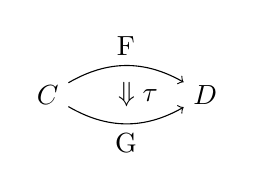
\begin{tikzpicture}
    \node (C) at (-1,0) {$\cat{C}$};
    \node (D) at (1,0) {$\cat{D}$};
    \node (T) at (0,0) {$\;\;\;\Downarrow\tau$};
    \draw[->,bend left] (C) to node [above] {F} (D);
    \draw[->,bend right] (C) to node [below] {G} (D);
  \end{tikzpicture}
\]
such that:
\begin{enumerate}
  \item $\forall X \in \cat{C},
    \exists \tau_X : F(X) \rightarrow G(X) \in \cat{D}$
  \item $\forall f : X \rightarrow Y \in \cat{C},
    \tau_Y \circ F(f) = G(f) \circ \tau_X$
\end{enumerate}
where the Morphism $\tau_X$ is called the \emph{Component} of $\tau$
at $X$. When (2) holds, a Commutative Diagram is formed and the
Morphisms $\tau_X$ are said to be \emph{Natural} in $X$. If there is
no Morphism in $\cat{D}$ corresponding to $\tau_X$, then there can
be no Natural Transformation from $F$ to $G$.

Milewski: A Natural Transformation maps Morphisms to Commuting
Diagrams

When every Component in $\tau$ is Invertible in $\cat{D}$, $\tau$ is a
\emph{Natural Isomorphism} (\S\ref{sec:natural_isomorphism}) and $F
\cong G$. Equivalently, a Natural Isomorphism is an Isomorphism in the
Functor Category $Fun(\cat{C},\cat{D})$.

Natural Isomorphisms:
\[
  Hom_\cat{Grp}(F_1,G) \cong U(G)
\]\[
  Hom_\cat{Set}(X,\cat{2}) \cong \pow(X)
\]\[
  Hom_\cat{BA}(B,\cat{2}) \cong Ult(X)
\]

in Programming Languages, Natural Transformations may be represented
as Polymorphic Functions (i.e. Family of Functions Parameterized by
Types)

Horizontal Composition (\S\ref{sec:horizontal_composition}):
Composition along $1$-morphisms (Functors)

Vertical Composition (\S\ref{sec:horizontal_composition}):
Composition along Objects (Categories)



% --------------------------------------------------------------------
\subsection{Vertical Composition}\label{sec:vertical_composition}
% --------------------------------------------------------------------

Given Natural Transformations $\eta : F \Rightarrow G$ and $\epsilon :
G \Rightarrow H$ between Functors $F,G,H : \cat{C} \rightarrow
\cat{D}$, the \emph{Vertical Composition} is $\epsilon\circ\eta : F
\Rightarrow H$:
\[
  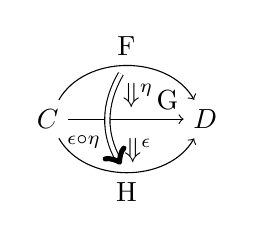
\begin{tikzpicture}
    \node (C) at (-1,0) {$\cat{C}$};
    \node (D) at (1,0) {$\cat{D}$};
    \node (N) at (0,0.3) {$\;\;\;\Downarrow^\eta$};
    \node (M) at (0,-0.4) {$\;\;\;\Downarrow^\epsilon$};
    \node (F) at (0,0.7) {};
    \node (H) at (0,-0.7) {};
    \draw[->,bend left=60] (C) to node [above] {F} (D);
    \draw[->] (C) to node [above] {\quad\quad\quad G} (D);
    \draw[->,bend right=60] (C) to node [below] {H} (D);
    \draw[->,bend right=30,double distance=1.5pt] (F) to
      node [left,pos=0.75] {$_{\epsilon\circ\eta}$} (H);
  \end{tikzpicture}
\]

Composition in the corresponding Functor Category



% --------------------------------------------------------------------
\subsection{Horizontal Composition}\label{sec:horizontal_composition}
% --------------------------------------------------------------------

Given Functors $F,G : \cat{C} \rightarrow \cat{D}$ and $J,K : \cat{D}
\rightarrow \cat{E}$, and Natural Transformations $\eta : F
\rightarrow G$ and $\epsilon : J \rightarrow K$, the \emph{Horizontal
  Composition} (or \emph{Godement Product}) is $\eta * \epsilon : JF
\Rightarrow KG$:
\[
  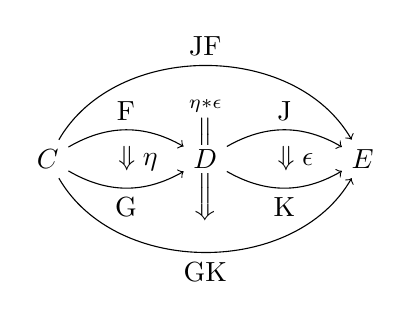
\begin{tikzpicture}
    \node (U) at (0,0) {$\stackrel{\eta*\epsilon}
      {\stackrel{\Big\|}{\Big\Downarrow}}$};
    \node [fill,color=white,scale=1.5] (W) at (0,0) {};
    \node (C) at (-2,0) {$\cat{C}$};
    \node (D) at (0,0) {$\cat{D}$};
    \node (E) at (2,0) {$\cat{E}$};
    \node (S) at (-1,0) {$\;\;\;\Downarrow\eta$};
    \node (T) at (1,0) {$\;\;\;\Downarrow\epsilon$};
    \draw[->,bend left] (C) to node [above] {F} (D);
    \draw[->,bend right] (C) to node [below] {G} (D);
    \draw[->,bend left] (D) to node [above] {J} (E);
    \draw[->,bend right] (D) to node [below] {K} (E);
    \draw[->,bend left=60] (C) to node [above] {JF} (E);
    \draw[->,bend right=60] (C) to node [below] {GK} (E);
  \end{tikzpicture}
\]

Horizontal Composition is Associative and has the same Identity as
Vertical Composition.



% --------------------------------------------------------------------
\subsection{Interchange Law}\label{sec:interchange_law}
% --------------------------------------------------------------------

Given three Categories, $\cat{B}$, $\cat{C}$, and $\cat{D}$,
and six Functors, $P,Q,R : \cat{B} \rightarrow \cat{C}$ and
$S,T,U : \cat{C} \rightarrow \cat{D}$, and four Natural
Transformations, $\sigma : P \rightarrow Q$, $\tau : Q \rightarrow R$,
$\sigma' : S \rightarrow T$, and $\tau' : T \rightarrow U$, the
following \emph{Interchange Law} applies:
\[
  (\tau' \cdot \sigma') \circ (\tau \cdot \sigma) =
  (\tau' \circ \tau) \cdot (\sigma' \circ \sigma)
\]



% --------------------------------------------------------------------
\subsection{Natural Isomorphism}\label{sec:natural_isomorphism}
% --------------------------------------------------------------------

\emph{Natural Equivalence} in a $1$-category %FIXME xref

\[
  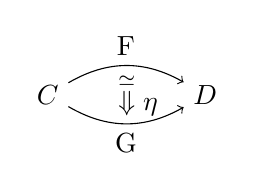
\begin{tikzpicture}
    \node (C) at (-1,0) {$\cat{C}$};
    \node (D) at (1,0) {$\cat{D}$};
    \node (N) at (0,0) {$\;\;\;\stackrel{\simeq}{\Downarrow}\eta$};
    \draw[->,bend left] (C) to node [above] {F} (D);
    \draw[->,bend right] (C) to node [below] {G} (D);
  \end{tikzpicture}
\]

\begin{itemize}
  \item Natural Isomorphism with a Two-sided Inverse (???)
  \item each Component $\eta_X : F(X) \rightarrow G(X)$ for all $X
    \in \cat{C}_0$ is an Isomorphism in $\cat{D}$
  \item Isomorphism in the Functor Category
    (\S\ref{sec:functor_category}) $[\cat{C},\cat{D}]$
\end{itemize}



% --------------------------------------------------------------------
\subsection{Extranatural Transformation}
\label{sec:extranatural_transformation}
% --------------------------------------------------------------------

For Functors $F : \cat{A} \times \cat{B}^{op} \times \cat{B}
\rightarrow \cat{D}$ and $G : \cat{A} \times \cat{C}^{op} \times
\cat{C} \rightarrow \cat{D}$, the Family $\eta(a,b,c) : F(a,b,b)
\rightarrow G(a,c,c)$ is Natural in $a$ and \emph{Extranatural} in $b$
and $c$ if the following holds:
\begin{itemize}
  \item (Natural in $a$): $\eta (-,b,c)$ is a Natural Transformation
  \item (Extranatural in $b$): $\forall (g:b \rightarrow b') \in
    \cat{B}_1, \forall a \in \cat{A}, \forall c \in \cat{C},
    \eta(a,b,c) \circ F(1,1,g) = \eta(a,b',c) \circ F(1,g,1)$
  \item (Extranatural in $c$): $\forall (h:c \rightarrow c') \in
    \cat{C}_1, \forall a \in \cat{A}, \forall b \in \cat{B}, G(1,h,1)
    \circ \eta(a,b,c) = G(1,1,h) \circ \eta(a,b,c')$
\end{itemize}



% --------------------------------------------------------------------
\subsection{Dinatural Transformation}
\label{sec:dinatural_transformation}
% --------------------------------------------------------------------

Ex.: Hughes Arrow (\S\ref{sec:hughes_arrow}) $\ggg : A (X,P) \times A
(P,Y) \rightarrow A (X,Y)$ is Dinatural in $P$. For each $f : P
\rightarrow Q$:
\[
  id \times A(f,id) \circ \ggg = A(id,f) \times id \circ \ggg
\]



% ====================================================================
\section{Opposite Category}\label{sec:opposite_category}
% ====================================================================

The \emph{Opposite} or \emph{Dual} (\S\ref{sec:abstract_category})
of a Category $\cat{C}$ is denoted $\cat{C^{op}}$ or
$\cat{C^*}$ and has the same Objects as $\cat{C}$ but the Domain
and Codomain in each Morphism is reversed. Objects and Morphisms of a
Dual Category may be written with over-lines to distinguish them from
the original Category: $\overline{f}: \overline{C} \rightarrow
\overline{D}$. With this notation the following Equalities may be
expressed:
\[
  1_{\overline{C}} = \overline{1_C}
\]\[
  \overline{f} \circ \overline{g} = \overline{g \circ f}
\]
A Terminal Object in $\cat{C}$ is an Initial Object in
$\cat{C^{op}}$ and vice-versa.

The Functor $(-)^\cat{op} : \cat{Cat} \rightarrow \cat{Cat}$
is an Involution (\S\ref{sec:involution}) but is Contravariant so it
does not define any Isomorphisms.

In a Dual Category the following are all Duals of eachother:
\begin{itemize}
  \item Monomorphisms and Epimorphisms (\S\ref{sec:morphism})
  \item Left and Right Inverses (\S\ref{sec:morphism})
  \item Initial and Terminal Objects (\S\ref{sec:universal_property})
\end{itemize}



% ====================================================================
\section{Category Product}\label{sec:category_product}
% ====================================================================

A \emph{Product}, $\times$, is a Construction (i.e. a Functor,
specifically a Bifunctor \S\ref{sec:bifunctor}) on Categories (or
Functors):
\[
  \times : \cat{Cat} \times \cat{Cat} \rightarrow \cat{Cat}
\]

Product (\S\ref{sec:product})



% --------------------------------------------------------------------
\subsection{Product Category}\label{sec:product_category}
% --------------------------------------------------------------------

A \emph{Product Category} can be constructed from two Categories,
$\cat{C}$ and $\cat{D}$, and is denoted:
\[
  \cat{C} \times \cat{D}
\]
has Objects of the form $(C,D)$ where $C \in \cat{C}$ and $D \in
\cat{D}$ and Morphisms $(f,g) : (C,D) \rightarrow (C',D')$ where $f
: C \rightarrow C' \in \cat{C}$ and $g : D \rightarrow D' \in
\cat{D}$. Composition and Identity are defined as:
\[
  (f',g') \circ (f,g) = (f' \circ f,g' \circ g)
\]\[
  1_{(C,D)} = (1_C, 1_D)
\]
$\cat{C} \times \cat{D}$ is a Product (\S\ref{sec:product}) in
$\cat{Cat}$.



\subsubsection{Projection}\label{sec:projection_functor}

A Product Category has a pair of \emph{Projections} which are Functors
from the Product Category to the original Categories:
\[
  \cat{C} \xleftarrow{\;\; P\;\;} \cat{C}\times\cat{D}
  \xrightarrow{\;\; Q\;\;} \cat{D}
\]
such that for $C,f \in \cat{C}, D,g \in \cat{D}$:
\[
  P(C,D) = C, \;\; P(f,g) = f
\]\[
  Q(C,D) = D, \;\; Q(f,g) = g
\]
Given any other Category, $\cat{B}$, there exists a unique Functor:
\[
  F : \cat{B} \rightarrow \cat{C} \times \cat{D}
\]
with:
\[
  PF = R : \cat{B} \rightarrow \cat{C}
\]\[
  QF = T : \cat{B} \rightarrow \cat{D}
\]
giving:
\[
  \forall h \in B, F(h) = (Rh,Th)
\]



% --------------------------------------------------------------------
\subsection{Functor Product}\label{sec:functor_product}
% --------------------------------------------------------------------

Give two Functors, $U : \cat{C} \rightarrow \cat{C'}$ and $V :
\cat{D} \rightarrow \cat{D'}$, a \emph{Functor Product} is
defined as:
\[
  U \times V : \cat{C} \times \cat{D}
  \rightarrow \cat{C'} \times \cat{D'}
\]
where:
\[
  (U \times V)(C,D) = (UC,VD), \;\; (U \times V)(f,g) = (Uf,Vg)
\]
and $(U \times V)$ is the unique Functor such that:
\[
  P'(U \times V) = UP, \;\; Q'(U \times V) = VQ
\]
%FIXME is the above correct?



% ====================================================================
\section{Quotient Category}\label{sec:quotient_category}
% ====================================================================

%FIXME this probably needs a rewrite

The \emph{Quotient Category} is defined for a Category $\cat{C}$
with Congruence Relation $\sim$ as $\cat{C}/\sim$:
\[
  (\cat{C}/\sim)_0 = \cat{C_0}
\]\[
  (\cat{C}/\sim)_1 = (\cat{C_1})/\sim
\]
where Morphisms are of the form $[f]$ where $f \in \cat{C_1}$.

For a Category $\cat{C}$ with Graph $G$ and relations $R$,
$\cat{C}/R$ is called the Category with \emph{Generators} $G$ and
\emph{Relations} $R$.

Homotopy Category (\S\ref{sec:homotopy_category})



% --------------------------------------------------------------------
\subsection{Congruence Category}\label{sec:congruence_category}
% --------------------------------------------------------------------

\emph{Congruence} on a Category is an Equivalence Relation on
Morphisms such that for two Morphisms $f,g \in \cat{C_1}$, $f \sim
g$ Implies:
\begin{itemize}
  \item $dom(f) = dom(g)$
  \item $cod(f) = cod(g)$
  \item $\forall a,b \in \cat{C_1}, bfa \sim bga$
\end{itemize}
Such a Congruence defines a \emph{Congruence Category}
$\cat{C^{\sim}}$:
\[
  (\cat{C^{\sim}})_0 = \cat{C}_0
\]\[
  (\cat{C^{\sim}})_1 = \{\langle f,g \rangle | f \sim g\}
\]\[
  \tilde{1_\cat{C}} = \langle 1_\cat{C}, 1_\cat{C} \rangle
\]\[
  \langle f',g' \rangle \circ \langle f,g \rangle = \langle f'f,g'g \rangle
\]
The Categorical Congruence $\sim$ on a Group $G$ is a Normal Subgroup
$N \subseteq G$ and the Quotient Category $G/\sim$ and the Quotient
Group $G/N$ coincide. \cite{awodey06}



% --------------------------------------------------------------------
\subsection{Kernel Category}\label{sec:kernel_category}
% --------------------------------------------------------------------

Given a Functor $F : \cat{C} \rightarrow \cat{D}$, a Congruence
$\sim_F$ on $\cat{C}$ is defined as:
\[
  f \sim_F g \leftrightarrow dom(f) = dom(g) \wedge cod(f) = cod(g)
  \wedge F(f) = F(g)
\]
The \emph{Kernel Category} of $F$ is then defined as the Congruence
Category of $\sim_F$
\[
  ker(F) = C^{\sim_F}
\]



% --------------------------------------------------------------------
\subsection{Finitely Presented Category}
\label{sec:finitely_presented}
% --------------------------------------------------------------------

% FIXME free category notation?
A \emph{Finitely Presented Category} is given by taking the Quotient
Category of a Free Category (\S\ref{sec:free_category})
$\cat{C}(G)$ with the Congruence $\sim_\Sigma$:
\[
  \cat{C}(G) / \sim_{\Sigma} = \cat{C}(G,\Sigma)
\]
where $\Sigma$ is the finite Set of Relations:
\[
  (g_1 \circ \ldots \circ g_n) = (g'_1 \circ \ldots \circ g'_m)
\]
for all $g_i \in G$ such that $dom(g_n) = dom(g'_m)$ and $cod(g_1) =
cod(g'_1)$.



% ====================================================================
\section{Arrow Category}\label{sec:arrow_category}
% ====================================================================

An \emph{Arrow Category} of a Category $\cat{C}$, written
$\cat{C^{\rightarrow}}$, has for its Objects the Morphisms of
$\cat{C}$ and as Morphisms pairs of Objects such that their
underlying Morphisms in $\cat{C}$ are Composable (Commutative
Squares).

The Arrow Category $\cat{C}^\rightarrow$ is Isomorphic to the
Functor Category $\cat{C^2}$.

There are two Functors defined on an Arrow Category:
\[
  \cat{C} \xleftarrow{\cat{dom}} \cat{C}^\rightarrow
  \xrightarrow{\cat{cod}} \cat{D}
\]

Equivalent to the Comma Category (\S\ref{sec:comma_category})
$(1_\cat{C}/1_\cat{C})$



% ====================================================================
\section{Comma Category}\label{sec:comma_category}
% ====================================================================

A \emph{Comma Category} is formed from a pair of Functors that share a
common Codomain. For three Categories, $\cat{A}$, $\cat{B}$, and
$\cat{C}$ and Functors $S$ (\emph{Source}) and $T$ (\emph{Target}) in
the following relation:
\[
  \cat{A} \xrightarrow{\;\; S\;\;} \cat{C} \xleftarrow{\;\;
    T\;\;} \cat{B}
\]
one can form a Comma Category $(S \downarrow T)$ with Objects as
Triples $(\alpha, \beta, f)$ where $\alpha$ is an Object in
$\cat{A}$, $\beta$ is an Object in $\cat{B}$, and $f : S(\alpha)
\rightarrow T(\beta)$ is a Morphism in $\cat{C}$ and with Morphisms
between Triples $(\alpha, \beta, f)$ to $(\alpha', \beta', f')$ as
pairs $(g,h)$ where $g : \alpha \rightarrow \alpha'$ is a Morphism in
$\cat{A}$ and $h : \beta \rightarrow \beta'$ is a Morphism in
$\cat{B}$.

When $S$ is a Functor, $\cat{1} \xrightarrow{\;\;S\;\;}
\cat{C}$, to a single Object $A \in \cat{C}$, the resulting
Comma Category may be denoted $(A \downarrow \cat{C})$ and is
called the Category of Objects under $A$. Here Objects are Morphisms
with Domain of $A$, and Morphisms are Commutative triangles with top
Vertex $A$.

The Category of Objects over $A$ is likewise $(\cat{C} \downarrow
A)$ and has as Objects Morphisms with Codomain $A$ and Morphisms are
Commutative triangles with a bottom Vertex $A$.

When both $S$ and $T$ are Functors from $\cat{1}$ to Objects $A$
and $B$ respectively, the result is a Discrete Category whose Objects
are $Hom(A,B)$.

The case where $S = T = 1_\cat{C}$, $(\cat{C} \downarrow
\cat{C})$, is the Category of all Morphisms of $\cat{C}$:
$\cat{C}^\cat{2}$.



% --------------------------------------------------------------------
\subsection{Slice Category}\label{sec:slice_category}
% --------------------------------------------------------------------

A \emph{Slice Category} (or \emph{Overcategory}) $\cat{C}/C$ of a
Category $\cat{C}$ with an Object $C$ has as Objects the Morphisms
with Codomain $C$ and as Morphisms those Morphisms in $\cat{C}$
between the Domains of the underlying Morphisms of the Objects of
$\cat{C}/C$. That is, for Objects in the Slice Category corresonding
to Morphisms $f$ and $f'$, the Morphism in the Slice Category between
the two is $g$ such that
\[
  f' \circ g = f
\]

\emph{Coslice}

if each Slice Category $\cat{C}/x$ is a Cartesian Monoidal Category
(\S\ref{sec:cartesian_monoidal}) then $\cat{C}$ is Locally Cartesian
(\S\ref{sec:locally_cartesian})

Categorical Semantics (\S\ref{sec:categorical_semantics}) for Formal
Logic (Part \ref{part:formal_logic}) and Type Theory (Part
\ref{part:type_theory})



% --------------------------------------------------------------------
\subsection{Coslice Category}\label{sec:coslice_category}
% --------------------------------------------------------------------



% ====================================================================
\section{Bifunctor}\label{sec:bifunctor}
% ====================================================================

A \emph{Bifunctor} is a Functor of two Variables from a Product
Category to an arbitrary Category:
\[
  B : \cat{C} \times \cat{D} \rightarrow \cat{A}
\]

A \emph{Multifunctor} is a generalized to $n$ or more Variables.



% --------------------------------------------------------------------
\subsection{Product Functor}\label{sec:product_functor}
% --------------------------------------------------------------------

\[
  \times : \cat{C} \times \cat{C} \rightarrow \cat{C}
\]

Category Product (\S\ref{sec:category_product})



% --------------------------------------------------------------------
\subsection{Coproduct Functor}\label{sec:coproduct_functor}
% --------------------------------------------------------------------

\[
  + : \cat{C} \times \cat{C} \rightarrow \cat{C}
\]



% --------------------------------------------------------------------
\subsection{Diagonal Functor}\label{sec:diagonal_functor}
% --------------------------------------------------------------------

For Functor Category (\S\ref{sec:functor_category})
$\cat{C}^\cat{J}$ with Small Index Category $\cat{J}$, a
\emph{Diagonal Functor} $\Delta : \cat{C} \rightarrow
\cat{C}^\cat{J}$ assigns to each Object $A$ of $\cat{C}$ the
Constant Functor $\Delta_A \in \cat{C}^\cat{J}$ with fixed $A$
and to each Morphism $f : A \rightarrow B$ of $\cat{C}$ the Natural
Transformation $\eta$ in $\cat{C}^\cat{J}$ given by $\eta_j =
f$.

If $\cat{J}$ is a Discrete Category with two Objects, the Diagonal
Functor is $\cat{C} \rightarrow \cat{C} \times \cat{C}$.

The Limit (\S\ref{sec:limit}) of a Functor $F : \cat{J} \rightarrow
\cat{C}$ is a Universal Morphism (\S\ref{sec:universal_morphism})
from the Diagonal Functor $\Delta$ to $F$.

If $\cat{C}$ is Complete (\S\ref{sec:complete_category}) then every
Functor from $\cat{J}$ to $\cat{C}$ has a Limit and the
operation of taking Limits is a Functor from $\cat{C}^\cat{J}$
to $\cat{C}$.

The Limit Functor is the Right-adjoint (\S\ref{sec:adjoint_functor})
of the Diagonal Functor.

A Colimit (\S\ref{sec:colimit}) is a Universal Morphism $F \rightarrow
\Delta$.

If $\cat{C}$ is Complete the Colimit Functor exists and is the
Left-adjoint of the Diagonal Functor.

As an example, the Diagonal Functor $\cat{C} \rightarrow \cat{C}
\times \cat{C}$ is the Left-adjoint of the Binary Product Functor
(\S\ref{sec:product_functor}) and the Right-adjoint of the Binary
Coproduct Functor (\S\ref{sec:coproduct_functor}).



% --------------------------------------------------------------------
\subsection{Profunctor}\label{sec:profunctor}
% --------------------------------------------------------------------

A \emph{Profunctor} (or \emph{Distributor}) is a Bifunctor that is
Contravariant in the first argument and Covariant in the second.

Generalization of Functors, Categorical generalization of Bimodules
(\S\ref{sec:bimodule})

$P : \cat{C} \nrightarrow \cat{D}$

$H_P : \cat{D}^{op} \times \cat{C} \rightarrow \cat{Set}$

Set of Heteromorphisms (\S\ref{sec:heteromorphism})

Identity Profunctor $Id : \cat{C} \nrightarrow \cat{C}$ is given by
the Hom-functor $\cat{C}(-,-) : \cat{C}^{op} \times \cat{C}
\rightarrow \cat{Set}$

Composition of Profunctors $P : \cat{C} \nrightarrow \cat{D}$, $Q :
\cat{D} \nrightarrow \cat{E}$:
\[
  Q P = \int^{d \in \cat{D}} P(d,-) \otimes Q(-,d)
\]
% FIXME kan extensions?

Every Functor $F : \cat{C} \rightarrow \cat{D}$ induces two
Profunctors $D(1,F) : \cat{C} \nrightarrow \cat{D}$ and $D(F,1)
: \cat{D} \nrightarrow \cat{C}$ where $D(1,F)(d,c) = D(d,f(c))$
and $D(f,1)(c,d) = D(f(c),d)$.

Functor $F : \cat{C} \rightarrow \cat{D}$ gives a Profunctor $P_F :
\cat{C} \nrightarrow \cat{D}$ by Post-composition with the Yoneda
Functor (\S\ref{sec:yoneda_embedding}):
\[
  P_F = Y_\cat{D} \circ F
\]



\subsubsection{Profunctor Bicategory}\label{sec:profunctor_bicategory}

Bicategory (\S\ref{sec:bicategory}) of Profunctors

Coend (\S\ref{sec:coend})



% ====================================================================
\section{Hom-functor}\label{sec:hom_functor}
% ====================================================================

A \emph{Hom-functor} is a Functor from a Locally Small Category
(\S\ref{sec:locally_small}), $\cat{C}$, to the Category $\cat{Set}$,
and has a Covariant and a Contravariant definition:

\begin{enumerate}
  \item \emph{Covariant Hom-functor}, for $A \in \cat{C}_0$, $f : X
    \rightarrow Y \in \cat{C}_1$:
\[
\begin{split}
  & h^A = Hom(A,-) : \cat{C} \rightarrow \cat{Set} \\
  & X \mapsto Hom(A,X) \\
  & f \mapsto Hom(A,f) : Hom(A,X) \rightarrow Hom(A,Y)
\end{split}
\]
  where $Hom(A,f)$ is defined for all $g \in Hom(A,X)$ as:
\[
  g \mapsto f \circ g
\]

  \item \emph{Contravariant Hom-functor} (also \emph{Functor of
    Points}, see Generalized Elements
    \S\ref{sec:generalized_element}), for $B \in \cat{C}_0$, $f : X
    \rightarrow Y \in \cat{C}_1$:
\[
\begin{split}
  & h_B = Hom(-,B) : \cat{C} \rightarrow \cat{Set} \\
  & X \mapsto Hom(X,B) \\
  & f \mapsto Hom(f,B) : Hom(Y,B) \rightarrow Hom(X,B)
\end{split}
\]
  where $Hom(f,B)$ is defined for all $g \in Hom(Y,B)$ as:
\[
  g \mapsto g \circ f
\]
\end{enumerate}

The Hom-functor $Hom(-,-)$ is a Covariant Bifunctor
(\S\ref{sec:bifunctor}):
\[
  Hom_\cat{C}(-,-):
    \cat{C}^{op} \times \cat{C} \rightarrow \cat{Set}
\]
each half of which is a Representable Functor
(\S\ref{sec:representable_functor}). $Hom_\cat{C}(-,-)$ is also the
Identity Profunctor (\S\ref{sec:profunctor}) $1_\cat{C} :
\cat{C} \nrightarrow \cat{C}$. Hom-functors are Continuous
Functors (\S\ref{sec:continuous_functor}).

The Category of all Hom-functors and Natural Transformations
(\S\ref{sec:natural_transformation}) between them, $\{ h^A | A \in
\cat{C} \}$, is a Subcategory of the Functor Category
(\S\ref{sec:functor_category}) $\cat{Set^C}$, and is Isomorphic to
$\cat{C^{op}}$ (see Yoneda Embedding \S\ref{sec:yoneda_embedding}).

Every Morphism $f : A' \rightarrow A$ determines a pair of Natural
Transformations:
\[
  Hom(f,-) : h^A \rightarrow h^{A'}
\]\[
  Hom(-,f) : h_{A'} \rightarrow h_A
\]

For any pair of Morphisms, $f : A' \rightarrow A$ and $g : B
\rightarrow B'$:
\[
  Hom(A',g) \circ Hom(f,B) = Hom(f,B') \circ Hom(A,g)
\]
is a path sending:
\[
  h : A \rightarrow B
\]
to:
\[
  g \circ h \circ f : A' \rightarrow B'
\]



% --------------------------------------------------------------------
\subsection{Closed Category}\label{sec:closed_category}
% --------------------------------------------------------------------

A \emph{Closed Category} is a Category $\cat{C}$ with:
\begin{itemize}
  \item Internal Hom-functor (\S\ref{sec:internal_hom}):
    \[
      [-,-]:\cat{C}^{op} \times \cat{C} \rightarrow \cat{C}
    \]
  \item Unit Object:
    \[
      I \in \cat{C}_0
    \]
  \item Natural Isomorphism:
    \[
      i : 1_\cat{C} \cong [I,-]
    \]
  \item Transformation:
    \[
      j_X : I \rightarrow [X,X]
    \]
    Extranatural (\S\ref{sec:extranatural_transformation}) in $X$
  \item Transformation:
    \[
      L_{Y Z}^X : [Y,Z] \rightarrow [[X,Y],[X,Z]]
    \]
    Natural in $Y$ and $Z$ and Extranatural in $X$
\end{itemize}
Satisfying the Axioms:
\begin{enumerate}
  \item $L_{Y Y}^X \circ j_Y = j_{[X,Y]}$ for any $X,Y$
  \item $[j_X,1] \circ L_{X Y}^X = i_{[X,Y]}$ for any $X,Y$
  \item $[i_Y,1] \circ L_{Y Z}^I = [1,i_Z]$ for any $Y,Z$
  \item $[1,L_{Y V}^X] \circ L_{U V}^Y = [L_{Y U}^X,1] \circ L_{[X,U]
    [X,V]}^{[X,Y]} \circ L_{U V}^X$ for any $X,Y,U,V$
  \item The Map $\gamma : \cat{C}(X,Y) \rightarrow \cat{C}(I,[X,Y])$
    defined by $f \mapsto [1,f](j_X)$ is a Bijection
\end{enumerate}

Every Closed Category embeds Fully and Faithfully into a Closed
Monoidal Category (\S\ref{sec:closed_monoidal}) by a Strong Closed
Functor (LaPlaza) %FIXME



\subsubsection{Internal Hom-functor}\label{sec:internal_hom}

\emph{Internal Hom Functor}
\[
  [-,-] : \cat{C}^{op} \times \cat{C} \rightarrow \cat{C}
\]



\subsubsection{Dualizing Object}\label{sec:dualizing_object}

\emph{Dualizing Object} $D$ in a Closed Category $\cat{D}$ is an
Object with Internal Hom $[-,D]: \cat{C} \rightarrow \cat{C}^{op}$ an
Involutive Duality Operation on $\cat{C}$: %FIXME
\[
  [[-,D],D]: \cat{C} \rightarrow \cat{C}
\]

Dual Object (\S\ref{sec:dual_object})



% --------------------------------------------------------------------
\subsection{Representable Functor}\label{sec:representable_functor}
% --------------------------------------------------------------------

%FIXME definition of 'representation'
%FIXME ref Naturally Isomorphic
Presheaf (\S\ref{sec:category_presheaf})

A Functor $F : \cat{C} \rightarrow \cat{Set}$ is a
\emph{Representable Functor} if it is Naturally Isomorphic to the
Hom-functor $h^A$ or $h_A$ for some Object $A \in \cat{C}$.

A \emph{Covariant Representable Functor} for an Object $A$ in a
Category $\cat{C}$ is defined as Naturally Isomorphic to the
Covariant Hom-functor $h^A = Hom(A,-) : \cat{C} \rightarrow
\cat{Set}$
\[
  Hom(A,-) : Hom(A,X) \xrightarrow{f_*} Hom(A,Y)
\]
A \emph{Contravariant Representable Functor} for $A$ is a Functor that
is Naturally Isomorphic to the Contravariant Hom-functor $h_A =
Hom(-,A) : \cat{C^{op}} \rightarrow \cat{Set}$
\[
  Hom(-,A) : Hom(X,A) \xrightarrow{f^*} Hom(Y,A)
\]

A \emph{Representation} of a Covariant Representable Functor, $F$, is
a pair $(A, \Phi)$ with Natural Isomorphism $\Phi : Hom(A,-)
\rightarrow F$.

Contravariant Representable Functors map all Colimits
(\S\ref{sec:colimit}) to Limits (\S\ref{sec:limit}).

A Locally Small Category (\S\ref{sec:locally_small}) has Representable
Functors for all Objects.

generalization of Upper Sets (\S\ref{sec:upper_set}) in Posets



% --------------------------------------------------------------------
\subsection{Locally Small Category}\label{sec:locally_small}
% --------------------------------------------------------------------

A Category is \emph{Locally Small} if all Hom-sets
(\S\ref{sec:hom_set}) of the Category are Sets and not Proper Classes.
% FIXME definition in terms of hom-sets

Hom-functor (\S\ref{sec:hom_functor})

There is at least one canonical Representable Functor
(\S\ref{sec:representable_functor}) from any Locally Small Category
into $\cat{Set}$.

For a Locally Small Category $\cat{C}$, $\cat{Set^{C^{op}}}$ is
Complete (\S\ref{sec:complete_category}) and Cocomplete
(\S\ref{sec:cocomplete_category}) and for all $C \in \cat{C}_0$,
the Evaluation Functor $ev_C : \cat{Set^{C^{op}}} \rightarrow
\cat{Set}$ preserves all Limits. \cite{awodey06}



% ====================================================================
\section{Concrete Category}\label{sec:concrete_category}
% ====================================================================

A \emph{Concrete Category} is pair, $(\cat{C},U)$, where $\cat{C}$ is
a Category and $U$ is a Faithful Functor
(\S\ref{sec:faithful_functor}) $U : \cat{C} \rightarrow \cat{Set}$.

Representable Functor (\S\ref{sec:representable_functor})

Sets with Structure (\S\ref{sec:abstract_structure})

Categories with Interpretations as Concrete Categories:
\begin{itemize}
  \item $\cat{Set}$
  \item $\cat{Top}$
  \item $\cat{Grp}$
\end{itemize}

Not \emph{Concretizable}:
\begin{itemize}
  \item $\cat{Toph}$
\end{itemize}



% ====================================================================
\section{Yoneda Lemma}\label{sec:yoneda_lemma}
% ====================================================================

For an arbitrary Covariant Functor $F : \cat{C} \rightarrow
\cat{Set}$:
\[
  Nat_\cat{Set^C}(h^A,F) \cong F(A)
\]
If $F$ is a Covariant Hom-functor $h^B$, then:
\[
  Nat_\cat{Set^C}(h^A,h^B) \cong Hom(B,A)
\]

For an arbitrary Contravariant Functor $G : \cat{C}^{op} \rightarrow
\cat{Set}$:
\[
  Nat_\cat{Set^{C^op}}(h_B,G) \cong G(A)
\]
If $F$ is a Contravariant Hom-functor $h_B$, then:
\[
  Nat_\cat{Set^{C^{op}}}(h_A,h_B) \cong Hom(A,B)
\]

Corollary:
\[
  yA \cong yB \Rightarrow A \cong B
\]



% --------------------------------------------------------------------
\subsection{Yoneda Embedding}\label{sec:yoneda_embedding}
% --------------------------------------------------------------------

The Fully Faithful Contravariant Functor $h^- : \cat{C} \rightarrow
\cat{Set^C}$ which maps each Object $A \in \cat{C}_0$ to the
Hom-functor $h^A$ and each $f \in \cat{C}_1$ to the Natural
Transformation $Hom(f,-)$ can also be interpreted as a Covariant
Functor $h^- : \cat{C^{op}} \rightarrow \cat{Set^C}$. Being a
Faithful Functor means $h^-$ gives an Embedding
(\S\ref{sec:category_embedding}) of $\cat{C^{op}}$ in
$\cat{Set^C}$.

By the Contravariant Yoneda's Lemma:
\[
  h_-: \cat{C} \rightarrow \cat{Set^{C^{op}}}
\]
called the \emph{Yoneda Embedding}.

Covariant:

$Nat_\cat{Set^C}(Hom(A,-), Hom(B,-)) \cong Hom_\cat{C}(B,A)$

Contravariant:

$Nat_\cat{Set^{C^op}}(Hom(-,A), Hom(-,B)) \cong Hom_\cat{C}(A,B)$

Yoneda Embedding preserves all Products and Exponentials in
$\cat{C}$.



% --------------------------------------------------------------------
\subsection{Coyoneda}\label{sec:coyoneda}
% --------------------------------------------------------------------

Free Functor (\S\ref{sec:free_functor})



% ====================================================================
\section{Functor Category}\label{sec:functor_category}
% ====================================================================

Given two Categories, $\cat{C}$ and $\cat{D}$, a \emph{Functor
  Category} is a Category with Objects as Functors $T : \cat{C}
\rightarrow \cat{D}$ and Morphisms as Natural Transformations
between Functors:
\[
  \cat{D}^{\cat{C}} = Fun(\cat{C},\cat{D})
\]

$[\cat{C},\cat{D}]$

A Hom-set in a Functor Category may be denoted:
\[
  Nat(S,T) = \cat{D}^{\cat{C}}(S,T) =
    \{ \tau | \tau : S \rightarrow T \}
\]

With Evaluation Functor $\eta : \cat{D^C} \times \cat{C} \rightarrow
\cat{D}$, $\cat{D^C}$ is an Exponential
(\S\ref{sec:category_exponential}) in $\cat{Cat}$ and $\cat{Cat}$ is a
Cartesian Closed Category (\S\ref{sec:cartesian_closed}).

The Functor Category $\cat{C^2}$ is Isomorphic to Arrow Categories
(\S\ref{sec:arrow_category}) $\cat{C}^\rightarrow$.

The Functor Category $\cat{C}^\cat{2}$ from the Discrete Category
$\cat{2}$ is equivalent to the Product Category $\cat{C} \times
\cat{C}$.

For any Discrete Category $I$:
\[
  \cat{C}^I \cong \prod_{i \in I} \cat{C}
\]

The Functor Category $\cat{Set}^\downdownarrows$ where
$\downdownarrows$ is the Category with two Objects and two Morphisms
between them ($* \rightrightarrows \star$) is equivalent to the
Category of Graphs and Graph Homomorphisms $\cat{Graph}$. Cf.
Simplicial Sets (\S\ref{sec:simplicial_set}).

A Functor Category into the Category $\cat{Set}$ is called a
\emph{Category Diagram} (\S\ref{sec:category_diagram}).
%FIXME terminology doesn't match



% --------------------------------------------------------------------
\subsection{Set-valued Functor Category}\label{sec:setvalued_functor}
% --------------------------------------------------------------------

A \emph{Set-valued Functor Category} (or \emph{Category of Diagrams})
is a Functor Category from a Category into the Category
$\cat{Set}$.

A Presheaf (\S\ref{sec:presheaf}) is an example of a Set-valued
(Contravariant) Functor Category from an Opposite Category into
$\cat{Set}$.



\subsubsection{Powerset Functor}\label{sec:powerset_functor}

$\pow : \cat{Set} \rightarrow \cat{Set}$

Functions $f : X \rightarrow Y$ to the Image Mapping $img(f) :
\pow(X) \rightarrow \pow(Y)$



% ====================================================================
\section{Presheaf Category}\label{sec:presheaf_category}
% ====================================================================

Objects: Functors $F: \cat{C}^{op} \rightarrow \cat{Set}$

Morphisms: Natural Transformations $\Phi : F \rightarrow G$

$Psh(\cat{C}) = [\cat{C}^{op},\cat{Set}]$



% --------------------------------------------------------------------
\subsection{Presheaf}\label{sec:category_presheaf}
% --------------------------------------------------------------------

A \emph{Presheaf} is a Contravariant Functor from an Opposite Category
to the Category $\cat{Set}$. A Presheaf is an example of a
Set-valued Functor Category (\S\ref{sec:category_diagram}) and gives a
Cartesian Closed Category (\S\ref{sec:cartesian_closed}).

Presheaf (Topology \S\ref{sec:presheaf})

$2$-presheaf (\S\ref{sec:2_presheaf})

Sheave (\S\ref{sec:sheave})



% --------------------------------------------------------------------
\subsection{Copresheaf}\label{sec:copresheaf}
% --------------------------------------------------------------------



% --------------------------------------------------------------------
\subsection{Representable Presheaf}\label{sec:representable_presheaf}
% --------------------------------------------------------------------

Limit (\S\ref{sec:limit})



% --------------------------------------------------------------------
\subsection{Graphic Category}\label{sec:graphic_category}
% --------------------------------------------------------------------

Class of Finite Monoids and Categories permitting a ``graphic
display'' via Presheaf (\S\ref{sec:presheaf}) Categories
(def. nCat Lab) % FIXME

Graphic Monoid (\S\ref{sec:graphic_monoid})



% ====================================================================
\section{Universal Property}\label{sec:universal_property}
% ====================================================================

Unique up to Unique Isomorphism



% --------------------------------------------------------------------
\subsection{Universal Mapping Property}
\label{sec:universal_mapping_property}
% --------------------------------------------------------------------

A \emph{Universal Mapping Property} is a Property in the Language of
Category Theory that defines a Mathematical Structure up to
Isomorphism. By relation to the Curry-Howard Correspondence, these
Isomorphisms are effectively two-way Rules of Inference.

\emph{Existence}

\emph{Uniqueness}

Universal Construction

Milewski: If a Universal Construction exists for all Diagrams of a
certain shape in a Category, it can also be defined through an
Adjunction (\S\ref{sec:adjunction})



% --------------------------------------------------------------------
\subsection{Universal Morphism}\label{sec:universal_morphism}
% --------------------------------------------------------------------

Given a Functor $S: \cat{D} \rightarrow \cat{C}$, an
\emph{Universal Morphism} to $S$ or \emph{Initial Morphism}, is an
Initial Object of the form $(Y',u)$ in the Comma Category
(\S\ref{sec:comma_category}) $(X \downarrow S)$ where $X \in
\cat{C}_0$, $u : X \rightarrow S(Y') \in \cat{C}_1$ and $X' \in
\cat{D}_0$.
%FIXME is X' initial and/or terminal in D?

$(Y', u)$ satisfies the \emph{Initial Property}:
\[
  \forall Z' \in \cat{D}, \forall f : X \rightarrow S(Z') \in
  \cat{C}, \exists! g : Y' \rightarrow Z' : S(g) \circ u = f
\]

The Dual concept of an Initial Morphism, an Universal Morphism from
$S$ or \emph{Terminal Morphism}, is a Terminal Object of the form
$(X',v)$ in the Comma Category $(S \downarrow X)$ where $v : S(X')
\rightarrow X \in \cat{C}$.

$(X',v)$ satisfies the \emph{Terminal Property}:
\[
  \forall Y' \in \cat{D}, \forall f : S(Y') \rightarrow X \in
  \cat{C}, \exists! g : Y' \rightarrow X' : v \circ S(g) = f
\]

%FIXME universality in terms of Hom sets



\subsubsection{Universal Element}\label{sec:universal_element}

\emph{Representable Functor} (\S\ref{sec:representable_functor})

For a Functor $H : \cat{D} \rightarrow \cat{Set}$, an
\emph{Universal Element} of $H$ is a pair of Objects $(A,X) \in
\cat{D}_0 \times \cat{Set}_0$ such that:
\[
  \forall (A',X') \in \cat{D}_0 \times \cat{Set}_0,
  \exists! f : A \rightarrow A' \in \cat{D} : H(f)(X) = X'
\]



% --------------------------------------------------------------------
\subsection{Global Element}\label{sec:global_element}
% --------------------------------------------------------------------

A \emph{Global Element}, $a$, (also \emph{Point} or \emph{Constant})
of an Object, $A$, is a Morphism from a Terminal Object, $1$, to that
Object
\[
  a: 1 \rightarrow A
\]
In $\cat{Set}$ this expresses an Isomorphism:
\[
  A \cong Hom_\cat{Set}(1,A)
\]
but is not true for all Categories in general.

In some settings Global Elements represent Closed Terms.

Pointed Object (\S\ref{sec:pointed_object})



\subsubsection{Well-pointed Category}\label{sec:well_pointed}

Well-pointed Topos (\S\ref{sec:wellpointed_topos})



% --------------------------------------------------------------------
\subsection{Generalized Element}\label{sec:generalized_element}
% --------------------------------------------------------------------

A \emph{Generalized Element} (or \emph{General Element} or
\emph{Variable}) $x$ is a Morphism from an arbitrary Domain Object,
$X$:
\[
  x: X \rightarrow A
\]

In some contexts Generalized Elements correspond to arbitrary Terms
(\S\ref{sec:term}) as in Programming Languages (``Computational
Trinitarianism'', Curry-Howard Correspondence
\S\ref{sec:curry_howard}).



% --------------------------------------------------------------------
\subsection{Separator}\label{sec:separator}
% --------------------------------------------------------------------

(or \emph{Generator})

nLab:

Object $S$ (or Family of Objects $\class{S}$) in a Category $\cat{C}$
for which Generalized Elements (\S\ref{sec:generalized_element}) with
Domain $S$ (or $\class{S}$) are ``sufficient'' to distinguish
Morphisms in $\cat{C}$.

Grothendieck Categories (\S\ref{sec:grothendieck_category})



\subsubsection{Coseparator}\label{sec:coseparator}



% --------------------------------------------------------------------
\subsection{Category Diagram}\label{sec:category_diagram}
% --------------------------------------------------------------------

A \emph{Category Diagram} is a Covariant Functor from an \emph{Index
  Category} into another Category:
\[
  D : \cat{J} \rightarrow \cat{C}
\]
A Diagram is the Category Theory analogue of an Indexed Family of Sets
(\S\ref{sec:index_set}).

Category of Diagrams (\S\ref{sec:setvalued_functor})

$Diag(\cat{C},\cat{D})$



\subsubsection{Cone}\label{sec:category_cone}

A \emph{Cone} in a Diagram $D : \cat{J} \rightarrow \cat{C}$ is
an Object $C \in \cat{C}_0$ and a Unique Morphism $c_j : C
\rightarrow D_j$ for each Object in the Diagram such that any
resulting triangles Commute.

This is equivalent to a Natural Tranformation from the Constant
Functor (\S\ref{sec:constant_functor}) $\Delta_C$ to the Diagram
Functor $D$.

Cone Category $\cat{Cone}(D)$

Cocone (\S\ref{sec:cocone})



\paragraph{Universal Cone}\label{sec:universal_cone}\hfill

Universal Object in the Cone Category

Cone Category $\cat{Cone}(D)$

A Limit (\S\ref{sec:limit}) is a Terminal Object in the Cone
Category.



\subsubsection{Cocone}\label{sec:cocone}

A \emph{Cocone} in a Diagram $D : \cat{J} \rightarrow \cat{C}$
is an Object $C \in \cat{C}_0$ and a Unique Morphism $c_j : D_j
\rightarrow C$ for each Object in the Diagram such that any resulting
triangle Commutes.




\paragraph{Universal Cocone}\label{sec:universal_cocone}\hfill

Universal Object in the Cocone Category

Cocone Category $\cat{Cocone}(D)$

A Colimit (\S\ref{sec:colimit}) is a Initial Object in the Cocone
Category.



\subsubsection{Wedge}\label{sec:wedge}

$T : \cat{C}^{op} \times \cat{C} \rightarrow \cat{D}$

\emph{Wedge}, $X \in \cat{D}$ with Family of Morphisms $\omega_C :
X \rightarrow T(C,C)$ in $\cat{D}$ for all $C \in \cat{C}$ such
that for any $f : C \rightarrow C'$ in $\cat{C}$:
\[
  \omega_C \circ T(1_C,f) = \omega_C' \circ T(f,1_{C'})
\]
(Extranatural Transformation \S\ref{sec:extranatural_transformation}

$\omega_C(X) = n_C : C \rightarrow C$ are Components of a Natural
Transformation from $1_\cat{C} \rightarrow 1_\cat{C}$. A Wedge
$X \xrightarrow{.} Hom : \cat{C}^{op} \times \cat{C} \rightarrow
\cat{Set}$ is a Function $X \rightarrow Nat
(1_\cat{C},1_\cat{C})$.

A Universal Wedge is called an \emph{End} (\S\ref{sec:end})



\subsubsection{Span}\label{sec:span}

\emph{Span} (or \emph{Roof} or \emph{Correspondence})

Span from Object $X$ to Object $Y$ in a Category $\cat{C}$, with
another Object $S$:
\[
  X \xleftarrow{\quad f \quad} S \xrightarrow{\quad g \quad} Y
\]

generalization of Relations: a Correspondence which is
$(-1)$-truncated (\S\ref{sec:truncation}) as a Morphism into the
Cartesian Product

Diagram over $1 \rightarrow 2 \leftarrow 3$

The Colimit of a Span is a Pushout (\S\ref{sec:pushout})

Spans can be Composed in a Category with Pullbacks
(\S\ref{sec:pullback})



\paragraph{Correspondence Category}\label{sec:correspondence_category}\hfill

Category of Spans

$\cat{Corr_C}$

Self-dual: if Limits Exist, Colimits also Exist and vice versa



\subsubsection{Cospan}\label{sec:cospan}

The Limit of a Cospan is a Pullback (\S\ref{sec:pullback})



\subsubsection{Category of Elements}\label{sec:element_category}

For all $P \in \cat{Set^{C^{op}}}$, $P$ is a Colimit of
Representable Functors:
\[
  \lim_{\rightarrow_j} yA_j \cong P
\]
by the Yoneda Lemma (\S\ref{sec:yoneda_lemma})

Index Category: $\int_\cat{C} P$

Objects: $(x,C)$ where $C \in \cat{C}_0$ and $x \in PC$

Morphisms: Triples $(h, (x',C'), (x,C))$ where $h : C' \rightarrow C
\in \cat{C}_1$ such that $P(h)(x) = x'$.

Projection Functor: $\pi : \int_\cat{C} P \rightarrow \cat{C}$
such that $\pi(x,C) = C$ and $\pi(h, (x',C'), (x,C)) = h$



% --------------------------------------------------------------------
\subsection{Limit}\label{sec:limit}
% --------------------------------------------------------------------

\emph{Limit} = \emph{Inverse Limit} = \emph{Projective Limit} =
\emph{Left Root}

\emph{Colimit} = \emph{Direct Limit} = \emph{Inductive Limit} =
\emph{Right Root}

Colimit (\S\ref{sec:colimit})

A \emph{Limit} is defined as a Terminal Object in the Cone Category
(\S\ref{sec:category_cone}) over a Diagram $D : \cat{J} \rightarrow
\cat{C}$:
\[
  c_i : \lim_{\xleftarrow[j]{}} D_j \rightarrow D_i
\]

A Category has all Finite Limits if and only if it has Finite Products
(\S\ref{sec:category_product}) and Equalizers (\S\ref{sec:equalizer}),
or equivalently if it has Pullbacks (\S\ref{sec:pullback}) and a
Terminal Object (\S\ref{sec:terminal_object}). Furthermore, a Category
has all Limits of som Cardinality if and only if it has all Equalizers
and Products of that Cardinality. \cite{awodey06}

A Limit is also definable as a Natural Isomorphism (a Natural
Transformation with every Component an Isomorphism) between the two
Functors:
\[
  \cat{C}(c, \lim_{\xleftarrow[j]{}} D) \cong Nat (\Delta_c, D)
\]

Representable Presheaf (\S\ref{sec:representable_presheaf})



\subsubsection{Finite Limit}\label{sec:finite_limit}

Limit over a Finite Diagram, i.e. one whose shape is a Finite Category
(\S\ref{sec:finite_category})



\subsubsection{Terminal Object}\label{sec:terminal_object}

An Object $1$ in a Category $\cat{C}$ is \emph{Terminal} if for
every other Object $A$ in the Category there is a unique Morphism $A
\rightarrow 1$. A Unique, Canonical Isomorphism exists between any two
Terminal Objects in $\cat{C}$.

As an example, in $\cat{Set}$ and $\cat{Pos}$, all Singleton
Sets are Terminal, and as such they are all Isomorphic to each other.
Given a Set $X$:
\[
  |X| = 1 \leftrightarrow \forall Y, |Hom_{\cat{Set}}(Y,X)| = 1
\]

In a Poset, a Top Element is a Terminal Object.



\subsubsection{Product}\label{sec:product}

A \emph{Product} of two Objects $P = A \times B$:
\[
  A \xleftarrow{\;\;p_1\;\;} P \xrightarrow{\;\;p_2\;\;} B
\]
is a Product of $A$ and $B$ if and only if for any $A
\xleftarrow{\;\;z_1\;\;} Z \xrightarrow{\;\;z_2\;\;} B$:
\[
  \exists!u : Z \rightarrow P
\]
with $p_i \circ u = z_i$. $u$ is called a \emph{Factorization} and may
also be written as $\langle z_1, z_2 \rangle$ as it is uniquely
determined by $z_1$ and $z_2$.

A Product of two Categories is uniquiely Isomorphic to the Cartesian
Product (\S\ref{sec:cartesian_product}) of the two Sets.

In a Poset, the Product of two Elements is the Meet or Greatest Lower
Bound (\S\ref{sec:greatest_lowerbound}).

For Morphisms $f$ and $g$, a Product $f \times g$ is defined where $f
: A \rightarrow A'$, $g : B \rightarrow B'$ and:
\[
  f \times g : A \times B \rightarrow A' \times B' =
  \langle f \circ p_1, g \circ p_2 \rangle
\]
with $p_1$ and $p_2$ the Projections $p_1 : A \times B \rightarrow A$
and $p_2 : A \times B \rightarrow B$.

A Category $\cat{C}$ with Binary Products between any two Objects
has a \emph{Product Functor} (\S\ref{sec:product_functor}):
\[
  \times : \cat{C} \times \cat{C} \rightarrow \cat{C}
\]
which Maps pairs of Objects of $\cat{C}$ to their Product:
\[
  (A,B) \mapsto A \times B
\]
and Morphisms of $\cat{C}$ to their Product:
\[
  (f,g) \mapsto f \times g
\]
A Category with Binary Products and a Terminal Object is said to have
all \emph{Finite Products}. It is possible to Model the Theory of
Groups (\S\ref{sec:group_theory}) in any Category with all Finite
Products.

A Category has Finite Products and Equalizers if and only if it has
Pullbacks (\S\ref{sec:pullback}) and a Terminal Object. \cite{awodey06}

Products are unique up to Isomorphism (\S\ref{sec:isomorphism}). The
Canonical Commutative Isomorphism $A \times B \cong B \times A$ is:
\[
  \langle p_2, p_1 \rangle : A \times B \rightarrow B \times A
\]
which is the Natural Transformation $\theta$ betwen the Product
Functor and the \emph{Twisted Product Functor} $\tilde{\times} :
\cat{C} \times \cat{C} \rightarrow \cat{C}$ (Mapping $(A,B)
\mapsto B \times A$):
\[
  \theta : \times \rightarrow \tilde{\times}
\]

The Universal Mapping Property for Products may be stated as a two-way
Rule of Inference:
\[
  {
    \frac{X \rightarrow A \;\;\;\; X \rightarrow B}
    {X \rightarrow A \times B}
  }\times
\]

Products are also Associative:
\[
  A \times (B \times C) \cong (A \times B) \times C
\]

In $\cat{Set}$ the Product is the Cartesian Product $\times$ and the
Unit is the Singleton Set $1$.

In $\cat{Rel}$ the Product is the Direct Sum $+$ and the Unit is
the Empty Set $\varnothing$.

In $\cat{Hilb}$ the Product is Binary Sum and the Unit is the
Zero-dimensional Hilbert Space $\{ 0 \}$. %FIXME products not
                                %isomorphic? strict monoidal category



\paragraph{N-ary Products}\label{sec:category_nary}\hfill
A Terminal Object is a \emph{Nullary Product}. A general Object is its
own \emph{Unary Product}.

By Associativity of Products, $A \times B \times C = (A \times B)
\times C$ so any Category that has Binary Products also has all
\emph{Finite N-ary Products}.



\paragraph{Diagonal}\label{sec:diagonal}\hfill

\emph{Diagonal} of an Object $X$ in a Category with Products is the
canonical Morphism:
\[
  \Delta : X \xrightarrow{(\Id,\Id)} X \times X
\]

\fist Cf. Codiagonal (\S\ref{sec:codiagonal})



\subsubsection{Equalizer}\label{sec:equalizer}

An \emph{Equalizer} is an (Unique) Object $E$ and Morphism $e: E
\rightarrow A$ such that for a given pair of Parallel Morphisms $f,g :
A \rightarrow B$:
\[
  f \circ e = g \circ e
\]
$e$ is necessarily a Monomorphism.

Limit of Parallel Morphisms

For a Set $X$ in $\cat{Set}$, every Subset $U \subseteq X$ occurs
as an Equalizer.

The Category $\cat{Ab}$ has all Equalizers.

If a Category has Binary Products (\S\ref{sec:category_product}) and
Equalizers then it has Pullbacks (\S\ref{sec:pullback}).



\paragraph{Kernel}\label{sec:morphism_kernel}\hfill

The \emph{Kernel} of a Morphism $f : X \rightarrow Y$ is the most
general Morphism $k : K \rightarrow X$ such that $fk = 0_{KY}$ and for
any Morphism $k' : K' \rightarrow X$ such that $fk' = 0_{K'Y}$, there
exists a unique Morphism $u : K' \rightarrow K$ such that $ku = k'$.

A Kernel is a special case of an Equalizer where one of the Morphisms
is a Zero Morphism (\S\ref{sec:zero_morphism}).



\paragraph{End}\label{sec:end}\hfill

\emph{End} of a Functor is a Universal Wedge (\S\ref{sec:wedge}) $E
\xrightarrow{.} T$ where $T : \cat{C}^{op} \times \cat{C}
\rightarrow \cat{D}$ and $E \in \cat{D}$

$\int_{C \in \cat{C}} T(C,C)$

The End of $Hom : \cat{C}^{op} \times \cat{C} \rightarrow
\cat{Set}$ is $Nat (1_\cat{C},1_\cat{C})$ called the
\emph{Hochschild Cohomology} \S\ref{sec:hochschild_homology} or
\emph{Symmetries} of $\cat{C}$.

For two Functors $F,G : \cat{C} \rightarrow \cat{E}$, the End for
the Functor $\cat{E}(F(-), G(-)) : \cat{C}^{op} \times
\cat{C} \rightarrow \cat{Set}$ is:
\[
  \int_{C \in \cat{C}} \cat{E}(F(C), G(C)) = Nat (F,G)
\]

Forgetful Functor, Tannakian Reconstruction
(\S\ref{sec:tannakian_category}) %FIXME tannakian reconstruction
Monoid $(M,\mu,\eta)$, $\int_{(M,\mu,\eta)} \cong M$



\subsubsection{Pullback}\label{sec:pullback}

For a Category $\cat{C}$, a \emph{Pullback} (or \emph{Fiber
  Product} or \emph{Cartesian Square}) of Morphisms $f : A \rightarrow
C$ and $g : B \rightarrow C$ are Morphisms $p_1 : P \rightarrow A$ and
$p_2 : P \rightarrow B$ with the Universal Property that $fp_1 =
g_p2$. This implies for any given $z_1 : Z \rightarrow A$ and $z_2 : Z
\rightarrow B$ such that $fz_1 = gz_2$, there is a Unique Morphism $u
: Z \rightarrow P$ such that $z_1 = p_1 u$ and $z_2 = p_2 u$.

Categorical Semantics of an Equation (\S\ref{sec:equation})

In $\cat{Set}$ a Pullback is a Subset of the Cartesian Product of two
Sets: for the Diagram with $A,B,C$ Sets and Functions $f : A
\rightarrow C$, $g : B \rightarrow C$, a Pullback is the Subset $X
\subseteq A \times B$ of Pairs $(a,b)$ such that $f(a) = g(b)$.

A Pullback is the Limit of a Cospan (\S\ref{sec:cospan}).

Subtyping (\S\ref{sec:subtype})

Type Inference (\S\ref{sec:type_inference}) (Unification)

generalization of Intersection (\S\ref{sec:set_intersection}) and
Inverse Image (\S\ref{sec:preimage})

Dependent Sum (\S\ref{sec:dependent_sum}) over the Dependent Equality
Type (\S\ref{sec:dependent_equality}):
\[
  \sum_{a:A} \sum_{b:B} (f(a) = g(b))
\]

A Category has Pullbacks and a Terminal Object if and only if it has
Finite Products (\S\ref{sec:category_product}) and Equalizers
(\S\ref{sec:equalizer}). \cite{awodey06}

Base Change Functor (\S\ref{sec:base_change})



\paragraph{Reindexed Family}\label{sec:reindexed_family}\hfill

Indexed Family (\S\ref{sec:indexed_family})



\paragraph{Display Map}\label{sec:display_map}\hfill

Display Map Category (\S\ref{sec:display_map_category}): Categorical
Semantics (\S\ref{sec:categorical_semantics}) of Dependent Types
(\S\ref{sec:dependent_type})

$b : B \rightarrow A$

$B \type$ Dependent on Variable of Type $A$:

$x:A \vdash B(x):\mathrm{Type}$



\subparagraph{Display Class}\label{sec:display_class}\hfill

For Category $\cat{C}$ a Class of Morphisms of $\cat{C}$, $\class{D}
\subset \cat{C}_1$, is a \emph{Class of Displays} if all Pullbacks
(\S\ref{sec:pullback}) of Elements of $\class{D}$ exist and belong to
$\class{D}$.



\subsubsection{Cotensor Product}\label{sec:cotensor_product}

Monoidal Category (\S\ref{sec:monoidal_category})



\paragraph{Power}\label{sec:power}\hfill

Covariant Powerset Functor % FIXME

Cumulative Hierarchy (\S\ref{sec:cumulative_hierarchy})

$Hom(X,\cat{2}) \cong \pow(X)$

Ultrafilters (\S\ref{sec:ultrafilter})

$Ult(B) \cong Hom_\cat{BA}(B,\cat{2})$

Adjoint Functors:

$Ult : \cat{BA}^{op} \rightarrow \cat{Set}$

$\pow^\cat{BA} : \cat{Set}^{op} \rightarrow \cat{BA}$

Natural Transformations (\S\ref{sec:natural_transformation}) from
Stone Duality (\S\ref{sec:stone_duality}):
\[
  \eta_X : X \rightarrow Ult(\pow(X))
\]\[
  \phi_B : B \rightarrow \pow(Ult(B))
\]

$\pow^\cat{BA} :
  \cat{Set}^{op}_{fin} \rightarrow \cat{BA}_{fin}$

$A : \cat{BA}^{op}_{fin} \rightarrow \cat{Set}_{fin}$
\emph{Atoms} of a Boolean Algebra:
\[
  A(\mathcal{B}) = \{ a \in \mathcal{B} \;|\;
    0 < a, (b < a \Rightarrow b = 0) \}
\]
There is an Isomorphism between Atoms $a$ of a Finite Boolean Algebra
$\mathcal{B}$ and Ultrafilters $U \subseteq \mathcal{B}$:
\[
  U \mapsto \bigwedge_{b \in U} b
\]\[
  a \mapsto \uparrow (a)
\]



\subsubsection{Inverse Limit}\label{sec:inverse_limit}



% --------------------------------------------------------------------
\subsection{Colimit} \label{sec:colimit}
% --------------------------------------------------------------------

Adjoint Functor (\S\ref{sec:adjoint_functor})

Diagonal Functor (\S\ref{sec:diagonal_functor})

Small Limit

A \emph{Colimit} is defined as a Universal Cone
(\S\ref{sec:universal_cone})

A Category has Finite Colimits if and only if it has Finite Coproducts
(\S\ref{sec:coproduct}) and Coequalizers (\S\ref{sec:coequalizer}).
Likewise, a Category has all Colimits of some Cardinality $\kappa$ if
and only if it has Coequalizers and Coproducts of Cardinality
$\kappa$.



\subsubsection{Initial Object}\label{sec:initial_object}

An Object $0$ in a Category $\cat{C}$ is \emph{Initial} if for
every other Object $A$ in the Category there is a unique Morphism $0
\rightarrow A$. A Unique Canonical Isomorphism exists between any two
Initial Objects in $\cat{C}$.

An Initial Object is the Colimit of the Empty Diagram $\varnothing
\rightarrow \cat{C}$

In $\cat{Set}$ the Empty Set is Initial as the only mapping from it
to any other Set is the Empty Function.

In a Poset, the Bottom Element is an Initial Object.

All Universal Properties are Initial Objects somewhere...
%FIXME catsters



\subsubsection{Coproduct}\label{sec:coproduct}

$X,Y \in \cat{C}_0$, $X \amalg Y \in \cat{C}_0$

The Diagram $A \xrightarrow{\;\;q_1\;\;} Q \xleftarrow{\;\;q_2\;\;} B$
is a \emph{Coproduct} $A + B$ if for any $A \xrightarrow{\;\;z_1\;\;}
Z \xleftarrow{\;\;z_2\;\;} B$:
\[
  \exists!u : Q \rightarrow Z
\]
with $u \circ q_i = z_i$. $u$ may also be written as $[ z_1, z_2 ]$
and Coprojections $q_i$ may be called \emph{Injections} (although they
are not necessarily Injective Morphisms).

The Universal Mapping Property for Coproducts may be stated as a
two-way Rule of Inference:
\[
  {
    \frac{A \rightarrow X \;\;\;\; B \rightarrow X}
    {A + B \rightarrow X}
  }+
\]

An example of a Coproduct in $\cat{Set}$ is the Disjoint Union
(\S\ref{sec:disjoint_union}) in Set Theory or the Tagged Union
(\S\ref{sec:sum_type}) in Type Theory. The Coproduct of a Monoid is
sometimes defined as a Tensor Product (\S\ref{sec:tensor_product}). In
a Poset the Coproduct of two Elements is the Join or Least Upper Bound
(\S\ref{sec:least_upperbound}).

\begin{itemize}
\item $\cat{Set}$: Disjoint Union (\S\ref{sec:disjoint_union})
\item $\cat{Pos}$: Join (Least Upper Bound
  \S\ref{sec:least_upperbound})
\item $\cat{Grp}$: Free Product (\S\ref{sec:free_product})
\item $\cat{Ab}$, $\cat{Vect}$: Direct Sum (\S\ref{sec:direct_sum})
\item $\cat{Top}$: Disjoint Union Topology
  (\S\ref{sec:disjoint_union_topology})
\item Pointed Spaces: Wedge Sum (\S\ref{sec:wedge_sum})
\item Type Theory: Sum Type (\S\ref{sec:sum_type})
\end{itemize}

In the Category $\cat{Ab}$ there is a Canonical
Isomorphism:\cite{awodey06}
\[
  A + B \cong A \times B
\]



\paragraph{Codiagonal}\label{sec:codiagonal}\hfill

\emph{Codiagonal} (or \emph{Fold Morphism}) of an Object $X$ in a
Category with Coproducts:
\[
  \nabla : X \amalg X \xrightarrow{(\Id,\Id)} X
\]

\fist Cf. Diagonal (\S\ref{sec:diagonal})



\subsubsection{Coequalizer}\label{sec:coequalizer}

An \emph{Coequalizer} is an (Unique) Object $Q$ and Morphism $q: B
\rightarrow Q$ such that for a given pair of Parallel Morphisms $f,g :
A \rightarrow B$:
\[
  q \circ f = q \circ g
\]
$q$ is necessarily an Epimorphism.

Colimit of Parallel Morphisms

A Coequalizer in a Category $\cat{C}$ is an Equalizer in
$\cat{C}$ and \emph{vice versa}.

The Categories $\cat{Set}$ and $\cat{Pos}$ have all
Coequalizers.

Quotient (\S\ref{sec:equivalence_class})



\paragraph{Quotient Object}\label{sec:quotient_object}\hfill

\paragraph{Cokernel}\label{sec:cokernel}\hfill

\paragraph{Coend}\label{sec:coend}\hfill

of a Functor $S : \cat{C}^{op} \times \cat{C} \rightarrow
\cat{X}$, a Pair $(d, \zeta)$ with Object $d \in \cat{X}_0$ and
Extranatural Transformation (\S\ref{sec:extranatural_transformation})
$\zeta : S \xrightarrow{..} d$



\subsubsection{Pushout}\label{sec:pushout}

A Pushout is the Colimit of a Span (\S\ref{sec:span})

$B +_A C \cong (B + C)/\sim$

In $\cat{Set}$ a Pushout is a Quotient of the Disjoint Union of two
Sets: in a Diagram with $A,B,C$ Sets and Functions $f : C \rightarrow
A$ and $g : C \rightarrow B$, the Pushout is the Disjoint Union $A +
B$ with $a \in A \sim b \in B$ when there Exists $x \in C$ such that
$f(x) = a$ and $g(x) = b$. When $C$ is the Intersection of $A$ and $B$
(and $f$ and $g$ are the Inclusions), the Pushout is equal to $A + B$.



\subsubsection{Tensor Product}\label{sec:tensor_product}

For a Monoidal Category (\S\ref{sec:monoidal_category}) $\cat{M}$,
a \emph{Tensor Product} is a Functor:
\[
  \otimes : \cat{M} \times \cat{M} \rightarrow \cat{M}
\]

Cartesian Product in $\cat{Set}$

``Freest'' Bilinear Operator (\S\ref{sec:bilinear_map}):
\begin{itemize}
\item Modules: Module Tensor (\S\ref{sec:module_tensor})
\item Vector Spaces (\S\ref{sec:vector_space}): Outer Product
  (\S\ref{sec:outer_product})
\end{itemize}

Vertically Categorified (\S\ref{sec:vertical_categorification}) Monoid



\paragraph{Copower}\label{sec:copower}\hfill

\paragraph{Tensorial Strength}\label{sec:tensorial_strength}\hfill

Natural Transformation $\tau_{A,B} : A \otimes F B \rightarrow F (A
\otimes B)$
%FIXME commutative diagrams

Strong Functor (\S\ref{sec:strong_functor})

Strong Monad (\S\ref{sec:strong_monad})



\subsubsection{Direct Limit}\label{sec:direct_limit}

\paragraph{$\omega$-colimit}\label{sec:omega_colimit}\hfill

$\omega$-colimit $G_\infty$

Forgetful Functor $U : \cat{Grp} \rightarrow \cat{Set}$ creates
$\omega$-colimits (and all Limits). \cite{awodey06}



\subsubsection{Cocomplete Category}\label{sec:cocomplete_category}

A \emph{Cocomplete Category} is a Category where all Small Colimits
exist.

For any Categories $\cat{C}$ and $\cat{D}$, if $\cat{D}$ is
Cocomplete, then the Functor Category $\cat{D^C}$ is Cocomplete and
for every $C \in \cat{C}$, the Evaluation Functor $ev_C :
\cat{D^C} \rightarrow \cat{D}$ preserves Colimits.

For any Locally Small Category (\S\ref{sec:locally_small})
$\cat{C}$ the Functor Category $\cat{Set^{C^{op}}}$ is
Cocomplete.

For a Cocomplete Category $\mathcal{E}$ and Functor $F : \cat{C}
\rightarrow \mathcal{E}$, there is a Unique (up to Natural
Isomorphism) Colimit Preserving Functor $F_! : \cat{Set^{C^{op}}}
\rightarrow \mathcal{E}$ such that $F_! \circ y \cong A$ where $y$ is
the Yoneda Embedding (\S\ref{sec:yoneda_embedding}).\cite{awodey06}
%FIXME what is `A` here?



% --------------------------------------------------------------------
\subsection{Zero Object}\label{sec:zero_object}
% --------------------------------------------------------------------

An Object that is both an Initial and a Terminal Object is called a
\emph{Zero Object} (or \emph{Null Object}). A Category with a Zero
Object is called a \emph{Pointed Category}
(\S\ref{sec:pointed_category}).

For a Zero Object, $Z \in \cat{C}$, there is a Unique Morphism
between any two Objects, $A, B \in \cat{C}$ called the
\emph{Composite} in $Z$:
\[
  A \rightarrow Z \rightarrow B
\]

In $\cat{Grp}$, a Trivial Group ${1}$ is a Zero Object.



\subsection{Pointed Category}\label{sec:pointed_category}



% --------------------------------------------------------------------
\subsection{Exponential}\label{sec:category_exponential}
% --------------------------------------------------------------------

Given a Category $\cat{C}$ with Binary Products between any two
Objects:
\[
  \exists \times_{A,B} \forall A,B \in \cat{C}
\]
an \emph{Exponential Object} (\S\ref{sec:exponential_object}) $B^A$
with a Universal Morphism (\S\ref{sec:universal_morphism}) (sometimes
called ``eval'' or ``apply''):
\[
  \epsilon : B^A \times A \rightarrow B
\]
such that:
\[
  \forall X, f \in \cat{C}, \exists ! \lambda f :
  \epsilon \circ (\lambda f \times 1_A) = f
\]
where $\lambda f \times 1_A : X \times A \rightarrow B^A \times A$ is
called the \emph{Exponential Transpose} of $f$. The Morphisms $f$ and
$\lambda f$ are called \emph{Exponential Adjoints}. The $\epsilon$
function is the Counit of the Adjunction (\S\ref{sec:adjunction}) between
the Product Functor and the Exponential Functor.

The Universal Mapping Property for Exponentials implies the two-way
Rule of Inference:
\[
  {
    \frac{X \times A \rightarrow B}
    {X \rightarrow B^A}
  }exp
\]
From this the following Two-way Inference Rule may be Derived:
\[
    \frac{1 \times A \rightarrow B}
    {1 \rightarrow B^A}
\]

An Exponential $B^A$ corresponds to the Function Space
(\S\ref{sec:function_space}) from $A$ to $B$. For $A,B \in
\cat{Set}_0$ in the Category of Sets, the Exponential $B^A$ is
equal to the Hom-set (\S\ref{sec:hom_set}) $Hom(A,B)$.

In a Poset such as a Propositional Calculus, the Exponential
corresponds to Implication:
\[
    \frac{x \leq b \Rightarrow a}
    {x \wedge a \leq b}
\]

Exponentials do not exists for Group Homomorphisms but they do for
Groupoids (\S\ref{sec:groupoid}).

A Category with an Exponential for any two Objects and a Terminal
Object (\S\ref{sec:terminal_object}) is a Cartesian Closed Category
(\S\ref{sec:cartesian_closed}). In a Cartesian Closed Category the
Functor sending $B$ to $B^A$ is the Right-adjoint Functor
(\S\ref{sec:adjoint_functor}) $- \times Y$ and there is a Bijection
between Hom-sets $Hom(X \times A, B)$ and $Hom(X, B^A)$:
\[
  Hom(X \times A, B) \cong Hom(X, B^A)
\]

An Exponential can also be introduced by a Morphism between Morphisms
called ``curry'' which is equivalent to $\lambda$ above:
\[
  curry : C^{A \times B} \rightarrow (C^B)^A
\]
In a Cartesian Closed Category such as Simply-typed Lambda Calculus
(\S\ref{sec:simply_typed}), all the Morphisms are Internal, so $curry$
corresponds to an Object:
\[
  curry : ((C^B)^A)^{C^{A \times B}}
\]



\subsubsection{Exponential Functor}\label{sec:exponential_functor}

$-^A : \cat{C} \rightarrow \cat{C}$



% --------------------------------------------------------------------
\subsection{Directed Limit}\label{sec:directed_limit}
% --------------------------------------------------------------------

Accessible Category (\S\ref{sec:accessible_category})



% --------------------------------------------------------------------
\subsection{Filtered Limit}\label{sec:filtered_limit}
% --------------------------------------------------------------------

Filtered Colimit

Accessible Functor (\S\ref{sec:accessible_functor})



% --------------------------------------------------------------------
\subsection{Biproduct}\label{sec:biproduct}
% --------------------------------------------------------------------

both Product (\S\ref{sec:product}) and Coproduct
(\S\ref{sec:coproduct})

Category with a Zero Object (\S\ref{sec:zero_object})

any Category with Biproducts is Semi-additive
(\S\ref{sec:semiadditive_category})



% --------------------------------------------------------------------
\subsection{Base Change}\label{sec:base_change}
% --------------------------------------------------------------------

For a Moprhism $f : X \rightarrow Y$ in a Category $\cat{C}$ with
Pullbacks (\S\ref{sec:pullback}), a \emph{Base Change Functor} is an
Induced Functor:
\[
  f^* : \cat{C}/Y \rightarrow \cat{C}/X
\]
of Slice Categories (\S\ref{sec:slice_category}) with:
\[
  f^* = (Z \xrightarrow{\alpha} C) \mapsto
    (X \times_\cat{C} Z \xrightarrow{\alpha^*} X)
\]
%FIXME

If $\cat{C}$ is a Topos then it refines to an Essential Geometric
Morphism (\S\ref{sec:essential_geometric})


Cobase Change

$f_! \dashv f^* \dashv f_*$

$\Sigma_f \dashv f^* \dashv \Pi_f$



\subsubsection{Dependent Product}\label{sec:dependent_product}

Dependent Product Type (\S\ref{sec:pi_type})

Category with all Dependent Products necessarily has all Pullbacks
(\S\ref{sec:pullback})



\subsubsection{Dependent Sum}\label{sec:dependent_sum}

Dependent Sum Type (\S\ref{sec:sigma_type})



% --------------------------------------------------------------------
\subsection{Dependency Morphism}\label{sec:dependency_morphism}
% --------------------------------------------------------------------

\emph{Trace Monoid} (\S\ref{sec:trace_monoid})



% --------------------------------------------------------------------
\subsection{Kan Extension}\label{sec:kan_extension}
% --------------------------------------------------------------------

Wiki: Generalizes the notion of Extending a Function defined on a
Subset to a Function defined on the whole Set.

Categories $\cat{A}, \cat{B}, \cat{C}$

Fuctors $X : \cat{A} \rightarrow \cat{C}, F : \cat{A} \rightarrow
\cat{B}$

Right Kan Extension $Ran$ of $X$ along $F$ is a Functor $R : \cat{B}
\rightarrow \cat{C}$ and a Natural Transformation $\eta : RF
\Rightarrow X$ and Couniversal such that for any Functor $M : \cat{B}
\rightarrow \cat{C}$ and Natural Transformation $\mu : MF \rightarrow
X$ there is a Unique Natural Transformation $\delta : M \rightarrow R$
such that:
\[
  \mu = \eta \circ \delta_F
\]
where $\delta_F$ is the Natural Transformation with $\delta_F(a) =
\delta (F a) : M F(a) \rightarrow RF(a)$ for any Object $a \in
\cat{A}_0$. The Functor $R$ may also be written $\mathrm{Ran}_F X$.

Left Kan Extension $Lan$

Adjoint (\S\ref{sec:adjunction}) as Kan Extension

Limit (\S\ref{sec:limit}) as Kan Extension

Codensity Monad (\S\ref{sec:codensity_monad})

``Constrained Optimization'' % FIXME



% ====================================================================
\section{Adjunction}\label{sec:adjunction}
% ====================================================================

% Adjointness

Two Functors $F : \cat{C} \rightarrow \cat{D}$ and $U : \cat{D}
\rightarrow \cat{C}$ are \emph{Adjoints} when there is a Natural
Isomorphism:
\[
  \Phi : Hom_\cat{D}(F C,D) \cong Hom_\cat{C}(C,U D) : \Psi
\]
is Natural in $C$ and $D$.


Milewski: If a Universal Construction (\S\ref{sec:universal_property})
exists for all Diagrams of a certain shape in a Category, it can also
be defined through an Adjunction


\textbf{Unit}

Natural Transformation:
\[
  \eta : 1_\cat{C} \rightarrow U F
\]

\fist Unit may be called ``Return'' or ``Pure'' in a Monad
(\S\ref{sec:monad})


\textbf{Counit}

Natural Transformation:
\[
  \epsilon : F U \rightarrow 1_\cat{D}
\]

\fist Counit may be called ``Extract'' in a Comonad


Milewski: Unit allows the ``introduction'' of $R \circ L$ anywhere
$\Id_\cat{D}$ would be used; Counit allows an ``elimination'' of the
Composition $L \circ R$ replacing it with $\Id_\cat{C}$. Every Monad
or Comonad may be ``Factorized'' (not necessarily uniquely) into a
pair of Adjoint Functors.


\textbf{Triangle Identities} (\S\ref{sec:triangle_identity})
\[
  \epsilon F \circ F \eta = 1_F
\]\[
  U \epsilon \circ \eta U = 1_U
\]


Universal Mapping Property (\S\ref{sec:universal_property}) for $\eta
: 1_\cat{C} \rightarrow U \circ F$ (Unit):
\begin{itemize}
\item For any $C \in \cat{C}$, $D \in \cat{D}$, $f : C
  \rightarrow U D$, there exists a unique $g : FC \rightarrow D$ such
  that:
  \[
    f = U g \circ \eta_C
  \]
\end{itemize}

Universal Mapping Property for $\epsilon : F \circ U \rightarrow
1_\cat{D}$ (Counit):
\begin{itemize}
\item For any $C \in \cat{C}$, $D \in \cat{D}$, $g : F C
  \rightarrow D$, there exists a unique $f : C \rightarrow U D$ such
  that:
  \[
    g = \epsilon_D \circ F f
  \]
\end{itemize}

Relation between Hom-set and Unit definitions:
\[
  \Phi(g) = U g \circ \eta_C
\]\[
  \eta_C = \Phi(1_{FC})
\]

Relation between (Inverse) Hom-set and Unit definitions:
\[
  \Psi (f) = \epsilon_D \circ F f
\]\[
  \epsilon_D = \Psi(1_{U D})
\]

When Unit and Counit are Natural Isomorphisms
(\S\ref{sec:natural_isomorphism}), the Adjunction is an \emph{Adjoint
  Equivalence} (\S\ref{sec:adjoint_equivalence}).

Free Functors (\S\ref{sec:free_functor}) are Left Adjoint to Forgetful
Functors (\S\ref{sec:forgetful_functor}): Free Functor $\dashv$
Forgetful Functor

In a Cartesian Closed Category (\S\ref{sec:cartesian_closed}), the
following Functors are Adjoints:
\[
  + \dashv \Delta \dashv \times
\]
and:
\[
  (-) \times A \dashv (-)^A
\]
In First-order Logic (Provability $\vdash$):
\[
  \exists \dashv \star \dashv \forall
\]

Adjoint Logic (\S\ref{sec:adjoint_logic})



% --------------------------------------------------------------------
\subsection{Adjoint Functor}\label{sec:adjoint_functor}
% --------------------------------------------------------------------

An \emph{Adjoint Functor} is the Categorical analog of the Existential
Quantifier in Logic (\S\ref{sec:quantifier}) and the Image Operation
along a Continuous Function in Topology (Part \ref{sec:topology}).

Left Adjoint Functors Preserve Colimits (\S\ref{sec:colimit}) and
Epimorphisms (\S\ref{sec:epimorphism})

Right Adjoint Functors Preserve Limits (\S\ref{sec:limit}) and
Monomorphisms (\S\ref{sec:monomorphism})

nLab:

Left and Right Adjoint Functors are ``best approximations'' of Weak
Inverses (\S\ref{sec:weak_inverse})

Left Adjoint: may be thought of as being defined ``Freely''; consists
of anything an Inverse might ``need'' regardless of whether it
``works''.

Right Adjoint: may be thought of as being defined ``Cofreely'';
consists of anything that ``works'' in an Inverse regardless of
whether it's ``needed''.

A Forgetful Functor (\S\ref{sec:forgetful_functor}) has as
Left-adjoint a Free Functor (\S\ref{sec:free_functor}) and as
Right-adjoint a Cofree Functor (\S\ref{sec:cofree_functor})

A Forgetful Functor $G$, forgetting some Constraint $C$, has a
Left-adjoint $F$ that is a ``Free $C$ Functor'' %FIXME



\subsubsection{Triangle Identity}\label{sec:triangle_identity}

\emph{Triangle Identity} (or \emph{Zigzag Identity})
\[
  \epsilon F \circ F \eta = 1_F
\]\[
  U \epsilon \circ \eta U = 1_U
\]



% --------------------------------------------------------------------
\subsection{Adjoint Equivalence}\label{sec:adjoint_equivalence}
% --------------------------------------------------------------------

``Coherent'', ``Structured'' Equivalence

Adjunction $F \dashv G$ where Unit and Counit are Natural Isomorphisms
(\S\ref{sec:natural_isomorphism})

Weak Inverse (\S\ref{sec:weak_inverse})



% --------------------------------------------------------------------
\subsection{Adjoint Triple}\label{sec:adjoint_triple}
% --------------------------------------------------------------------

\subsubsection{Adjoint Cylinder}\label{sec:adjoint_cylinder}

Adjoint Triple such that the outer two Adjoints are Full
(\S\ref{sec:full_functor}) and Faithful (\S\ref{sec:faithful_functor})
Functors

Equivalently: the Induced Adjoint Pair on the Codomain of these
Inclusions (???) consists of an Idempotent Monad and Comonad (Adjoint
Monads \S\ref{sec:adjoint_monad})

Adjoint Modalities (\S\ref{sec:adjoint_modality})



% --------------------------------------------------------------------
\subsection{Reflection}\label{sec:reflection_adjunction}
% --------------------------------------------------------------------

\cite{winskel-nielsen93}

Right-adjoint is Full and Faithful



% --------------------------------------------------------------------
\subsection{Coreflection}\label{sec:coreflection_adjunction}
% --------------------------------------------------------------------

\cite{winskel-nielsen93}

Left-adjoint is Full and Faithful



% ====================================================================
\section{Monad}\label{sec:monad}
% ====================================================================

A \emph{Monad} is given by the Triple:
\[
  (T, \eta, \mu)
\]
where $T : \cat{C} \rightarrow \cat{C}$ is an Endofunctor and $\eta :
1_\cat{C} \rightarrow T$ and $\mu : T^2 \rightarrow T$ (where $T^2 = T
\circ T : \cat{C} \rightarrow \cat{C}$) are Natural Transformations,
called \emph{Unit} and \emph{Multiplication} resp., satisfying the
Coherence Conditions (\S\ref{sec:coherence_condition}):
\begin{enumerate}
  \item $\mu \circ T\mu = \mu \circ \mu T : T^3 \rightarrow T$
  \item $\mu \circ T\eta = \mu \circ \eta T = 1_T : T \rightarrow T$
\end{enumerate}
(1) is analogous to Associativity in Monoids and (2) gives the
existence of an Identity Element.

For every Object $X \in \cat{C}_0$, the Component of the Unit at $X$
is a Morphism:
\[
  \eta_X : X \rightarrow T (X)
\]

Horizontal Categorification (\S\ref{sec:horizontal_categorification})
of a Monoid

A Monad on $\cat{C}$ can be defined as a Monoid Object
(\S\ref{sec:monoid_object}) on the Endofunctor Category
(\S\ref{sec:endofunctor_category}) $\cat{End_C}$.

special case of a Hughes Arrow (\S\ref{sec:hughes_arrow}) with
``output'' but no ``input''

Pointed Endofunctor (\S\ref{sec:pointed_endofunctor}) $S : \cat{C}
\rightarrow \cat{C}$ with Natural Transformation $\sigma : 1_\cat{C}
\rightarrow S$ as the Unit; Well-pointed exactly when the Monad is
Idempotent (\S\ref{sec:idempotent_monad})

A Monad $T$ also arises as a Composition $G \circ F$ of Adjoint
Functors $F : \cat{C} \rightarrow \cat{D}$ and $G : \cat{D}
\rightarrow \cat{C}$, namely $T = G \circ F$ and the Unit of the Monad
is equivalent to the Unit of the Adjunction. If $F$ and $G$ are
Inverses then the corresponding Monad is the Identity Functor.

Given a Monad $T$ on a Category $\cat{C}$, there is a Category of
Adjunctions (\S\ref{sec:adjunction}) that give rise to that Monad.

A $T$-algebra (\S\ref{sec:t_algebra}) for a Monad $T$ is a Model
(\S\ref{sec:model}) of the Algebraic Theory
(\S\ref{sec:algebraic_theory}) given by a Monad.

Correspondences: \cite{jacobs-heunen-hasuo09}
\begin{itemize}
\item Monoids in $\cat{Cat}(\cat{C},\cat{C})$
\item Monads $M$ on $\cat{C}$
\item Identity-on-objects Functors $J : \cat{C} \rightarrow \cat{D}$
  having Right Adjoints (see Kleisli Categories
  \S\ref{sec:kleisli_category})
\end{itemize}

In Programming: Interface to Abstract Datatype
(\S\ref{sec:abstract_type}) of ``Program Fragments''

$\mathsf{return} : X \rightarrow T(X)$ (Comonad: $\textsf{extract}$)

$\mathsf{join} : T(T(X) \rightarrow T(X)$ (Comonad:
$\textsf{duplicate} : T(X) \rightarrow T(T(X))$)

$\mathsf{bind} : T(X) \rightarrow (X \rightarrow T(Y)) \rightarrow
T(Y)$ (Comonad: $\mathsf{cobind} : T(X) \rightarrow (T(X) \rightarrow
Y) \rightarrow T(Y)$)

An alternative to Monads for Computational Effects
(\S\ref{sec:computational_effect}) is Algebraic Effects
(\S\ref{sec:algebraic_effect}), more often seen in Strict Languages
(Algebraic Effects as a Subclass of Computational Effects
\cite{plotkin-pretnar09})

Layered Monads (\S\ref{sec:layered_monad}) \cite{filinski99}

\fist See also Graded Monads (\S\ref{sec:graded_monad}), Parametric
Effect Monads (\S\ref{sec:parametric_effect_monad}), Joinads
(\S\ref{sec:joinad})

Pointed Endofunctor (\S\ref{sec:pointed_endofunctor}) where $\sigma$
is the Unit

Operads (\S\ref{sec:operad}) ``Operations Monads''


\asterism


Comonad (\S\ref{sec:comonad})

Monadic Adjunction (\S\ref{sec:monadic_adjunction})

Terminal Object %FIXME terminal object required in category?

Generalization of Closure Operators on Posets (\S\ref{sec:poset}) to
arbitrary Categories (Galois Connections \S\ref{sec:galois_connection}
as Adjoint Pairs)

Continuation (\S\ref{sec:continuation}), Continuation Monad (???) %FIXME


\asterism


Computations

Monad: $(T,\eta,\mu)$

Type of $T$-computations with Values in $X$:
\[
  T (X)
\]

$\eta$ is a Family of Value-inclusion Functions $\eta_X : X
\rightarrow T X$

$\mu$ is a Family of Binding Functions $\mu_{X,Y} : T X \times (X
\rightarrow T Y) \rightarrow T Y$ such that for any $f : X \rightarrow
T Y$ and $g : Y \rightarrow T Z$:
\[
 (\eta a) \mu f = f a
\]\[
  t \mu \eta = t
\]\[
  (t \mu f) \mu g = t \mu (\lambda a.f a \mu g)
\]

For $f : X \rightarrow Y$:
\[
  T f = \lambda t.t \mu (\eta \circ f) : T X \rightarrow T Y
\]

Elements of $T X$ as Effectful Computations
(\S\ref{sec:computational_effect}) yielding Values in $X$

$\eta a$: Trivial (Effect-free) Computation of $a$


Kleisli Functions:
\[
\begin{split}
  f : X \rightarrow T(Y) \\
  g : Y \rightarrow T(Z)
\end{split}
\]

Kleisli Composition (``Bind'', $\mathtt{(\bindop)}$):
\[
  g \circ f : X \rightarrow T(Z)
  g \circ f = \mu_Z \circ T(g) \circ f
\]

Unit for Kleisli Composition (``Return''):
\[
  \mathtt{pure}_X : X \rightarrow T (X)
\]


\asterism

\cite{jones95}

Classes of Monads defined by Constructor Classes
(\S\ref{sec:constructor_class})
%FIXME

Composition of Monads $S$, $T$ of Value $A$:

$\mathsf{fcomp}\;S\;T\;A = T (S A)$ -- \emph{Forward Composition}

$\mathsf{bcomp}\;S\;T\;A = S (T A)$ -- \emph{Backward Composition}

(functor instances)

two Monads $S$,$T$ can be Composed if there is a $\mathsf{swap}$
Function:
\begin{flalign*}
  \quad\quad \mathsf{swap} & : S (T A) \rightarrow T (S A) &
\end{flalign*}
Satisfying Laws: %FIXME

(laws)

\begin{flalign*}
  \quad\quad \unit_{S,T} & : A \rightarrow S (T A) & \\
  \quad\quad \unit_{S,T} & = \unit_S \circ \unit_T &
\end{flalign*}

\begin{flalign*}
  \quad\quad \mathsf{join} & : S (T (S (T A))) \rightarrow S (T A) &
\end{flalign*}

\cite{duponcheel-jones93}

Premonad (???) %FIXME

Definition of $\mathsf{join}$ is not possible using only the
Operations of the two Monads, additional constructions linking the two
components is required.

\cite{duponcheel-jones93} give four possible constructions:
\begin{enumerate}
  \item Trivial: Premonads $S$ and $T$; $\mathsf{join}$ given by
    definition as a Polymorphic Function
  \item $\mathsf{prod}$ Construction: Monad $S$, Premonad $T$ %FIXME
  \item $\mathsf{dorp}$ Construction: Premonad $S$, Monad $T$ %FIXME
  \item $\mathsf{swap}$ Construction: Monads $S$ and $T$ %FIXME
\end{enumerate}

Into/Outof %FIXME

Combining two arbitrary Monads involves using one fixed Monad to
Transform another arbitrary Monad


\textbf{Monad Transformers}

%FIXME section?

Constructors with Kind $(\star \rightarrow \star) \rightarrow (\star
\rightarrow \star)$:

Examples:
\begin{align*}
  \mathsf{MaybeT} & = \mathsf{fcomp\;Maybe} \\
  \mathsf{ErrorT} & = \mathsf{fcomp\;Error} \\
  \mathsf{WriterT} & = \mathsf{fcomp\;Writer} \\
  \mathsf{ReaderT}\; r & = \mathsf{bcomp}\;(r \rightarrow)
\end{align*}

Class of Monad Transformers:
\begin{flalign*}
  \quad\quad & \mono{class}\;\mathsf{MonadT}\;t\;\mono{where} & \\
  \quad\quad & \quad \mathsf{lift} : m\;a \rightarrow t\;m\;a
\end{flalign*}
where $m$ is Constrained to be a Monad.


\asterism


\textbf{Generalization of Universal Algebra}

Any Variety (\S\ref{sec:variety}) in Universal Algebra gives rise to a
Monad on $\cat{Set}$ and the Algebra Type can be recovered from the
Monad as the Category of Eilenberg-Moore Algebras
(\S\ref{sec:eilenberg_moore}). A Variety of Algebras is a Finitary
Algebraic Category (\S\ref{sec:finitary_algebraic_category}).

A Monad on $\cat{Set}$:
\[
  (\pow, \{-\}, \bigcup)
\]
where $\pow$ is the Powerset Operation, $\{-\}$ is the
Singleton Operation, and $\bigcup$ is the Union Operation.
% FIXME xref


\asterism


Cayley's Theorem (\S\ref{sec:cayleys_theorem}): every Group is a
Subgroup of a Canonical Group of Permutations
(\S\ref{sec:permutation_group})

Yoneda Lemma (\S\ref{sec:yoneda_lemma}): every Category is a
Subcategory of a Canonical Functor Category
(\S\ref{sec:functor_category})

Filinski \cite{filinski99}/Piponi: every Monad is a Submonad of a
Canonical Continuation (\S\ref{sec:continuation}) Monad



% --------------------------------------------------------------------
\subsection{Monad Morphism}\label{sec:monad_morphism}
% --------------------------------------------------------------------

% --------------------------------------------------------------------
\subsection{$T$-algebra}\label{sec:t_algebra}
% --------------------------------------------------------------------

Monad $(T, \eta, \mu)$ where $T : \cat{C} \rightarrow \cat{C}$

$T$-algebra $(A, \theta)$ where $A \in \cat{C}$ and \emph{Action}
$\theta : T A \rightarrow A$ such that $\theta \circ \eta = 1_A$ and
$\theta \circ \mu_A = \theta \circ T \theta$

A $T$-algebra defines a Monoid with Underlying Set $A$ and Monoid
Operation $\theta$.

The $T$-algebras for a given Monad gives a Category of $T$-algebras,
$\cat{Alg}(T)$ (or $\cat{C}^T$, see Eilenberg-Moore Category
\S\ref{sec:eilenberg_moore}), where Morphisms between $T$-algebras
$(A, \theta)$ and $(B, \varphi)$ with $f : A \rightarrow B$ give a
Commutative Square:
\[
  \varphi \circ T f = f \circ \theta
\]
which is the Terminal Object in the Category of Adjunctions that give
rise to $T$.

also an Algebra over a Pointed Endofunctor ($S$-algebra
\S\ref{sec:s_algebra})

without Associativity: Algebra over an Endofunctor
($F$-algebra \S\ref{sec:f_algebra})



\subsubsection{$T$-algebra Presentation}
\label{sec:t_algebra_presentation}

nLab:

Presentation (\S\ref{sec:presentation})

Category $\cat{C}$

Monad $T$

$T$-algebra $\struct{A}$

$G \in \cat{C}_0$ Object of Generators

$R \in \cat{C}_0$ Object of Relations

Coequalizer (\S\ref{sec:coequalizer}) Diagram:
\[
  T R \rightrightarrows T G \rightarrow A
\]
in the Category $\cat{C}^T$ of $T$-algebras. %FIXME

generalized to any Concrete Category (\S\ref{sec:concrete_category})
with Free Objects (\S\ref{sec:free_object}) %FIXME

Category Presentation (\S\ref{sec:category_presentation})



% --------------------------------------------------------------------
\subsection{Idempotent Monad}\label{sec:idempotent_monad}
% --------------------------------------------------------------------

exactly when underlying Pointed Endofunctor
(\S\ref{sec:pointed_endofunctor}) is Well-pointed

nLab:

Idempotent Monad $(T, \eta, \mu)$ on Category $\cat{C}$, for an Object
$C \in \cat{C}_0$ the following are equivalent:
\begin{enumerate}
  \item $C$ carries a $T$-algebra Structure (\S\ref{sec:t_algebra})
  \item the Unit $\eta C : C \rightarrow T C$ is a Split Monomorphism
    (\S\ref{sec:split_monomorphism})
  \item the Unit $\eta C$ is an Isomorphism: Implies there is at most
    one Algebra Structure on $C$ given by $\xi = (\eta C)^{-1} : T C
    \rightarrow C$ %FIXME
\end{enumerate}



% --------------------------------------------------------------------
\subsection{Finitary Monad}\label{sec:finitary_monad}
% --------------------------------------------------------------------

(or \emph{Algebraic Monad})

is a Monoid in the Category of Algebraic Endofunctors (???) on
$\cat{Set}$

completely determined by Value on all Finite Ordinals $n \in \nats_0$
(as Finite Sets): $T(n)$ is the Set of $n$-ary Operations

\fist Cf. Non-symmetric Operad (\S\ref{sec:operad}) in
$\cat{Set}$


\asterism


Algebraic Theory (\S\ref{sec:algebraic_theory})

nLab:

Every Finitary Monad $T$ defines a Lawvere Theory
(\S\ref{sec:lawvere_theory}) $\mathrm{Th}_T$:
\[
  \cat{Th}_T = \cat{Free}^{op}_{fin}
\]
where $\cat{Free}_{fin}$ is the Category of Free Algebras $T(n)$ on
Finite Sets (as a Full Subcategory \S\ref{sec:full_subcategory} of
$\cat{Alg}_T$) %FIXME xref Alg_T

Equivalence between Category of Finitary Monads on $\cat{Set}$ and the
Category of Lawvere Theories %FIXME

Category of $T$-algebras is Equivalent to the Category of Models of
$\cat{Th}_T$ %FIXME

Commutative Algebraic Theory
(\S\ref{sec:commutative_algebraic_theory})

Category of Finitary Monads on $\cat{Set}$

Monadic over the Category of Finitary Endofunctors of $\cat{Set}$

Monadic over the Category of $\nats$-indexed Sets



% --------------------------------------------------------------------
\subsection{Submonad}\label{sec:submonad}
% --------------------------------------------------------------------

Subobject (\S\ref{sec:subobject})



% --------------------------------------------------------------------
\subsection{Applicative Monad}\label{sec:applicative_monad}
% --------------------------------------------------------------------

Applicative Functors? (\S\ref{sec:applicative_functor})

Applicative Comonad (\S\ref{sec:applicative_comonad})



% --------------------------------------------------------------------
\subsection{Cartesian Monad}\label{sec:cartesian_monad}
% --------------------------------------------------------------------

Multicategories (\S\ref{sec:multicategory})

Locally Cartesian Category (\S\ref{sec:locally_cartesian}), Pullbacks
(\S\ref{sec:pullback})



% --------------------------------------------------------------------
\subsection{Eilenberg-Moore Category}\label{sec:eilenberg_moore}
% --------------------------------------------------------------------

$\cat{C}^T$ Category of $T$-algebras (\S\ref{sec:t_algebra}) for
Monad $T$ in Category $\cat{C}$

Freely Constructed

$A \mapsto \mu_A : T^2 A \rightarrow T A$ is a Functor from
$\cat{C}$ to $\cat{C}^T$

$\theta : T A \rightarrow A \mapsto A$ is a Functor from
$\cat{C}^T$ to $\cat{C}$

Terminal Object in the Category of Adjunctions
(\S\ref{sec:adjoint_category}) that give rise to Monad $T$



% --------------------------------------------------------------------
\subsection{Kleisli Category}\label{sec:kleisli_category}
% --------------------------------------------------------------------

For Monad $T$ and Category $\cat{C}$, a \emph{Kleisli Category}
$\cat{C}_T$ (or $Kl(T)$) is equivalent to the Category of Free
$T$-algebras (\S\ref{sec:t_algebra})-- Full Subcategory
(\S\ref{sec:full_subcategory}) of Eilenberg-Moore Category
$\cat{C}^T$

Objects are Objects of $\cat{C}$ and Morphisms for a pair of
Objects $A$, $B$ are the Morphisms in $\cat{C}(A, T B)$

Composition of $f : A \rightarrow B$, $g : B \rightarrow C$ is $f
\circ T g \circ \mu_A : A \rightarrow TC$

Identity $\eta_A : A \rightarrow T A$

Initial Object in the Category of Adjunctions
(\S\ref{sec:adjoint_category}) that give rise to Monad $T$

The analogous construction for Hughes Arrows
(\S\ref{sec:hughes_arrow}) are Freyd Categories
(\S\ref{sec:freyd_category}).

Monad: $T$

Type of $T$-computations with Values in $X$:
\[
  T (X)
\]

Kleisli Functions:
\[
\begin{split}
  f : X \rightarrow T(Y) \\
  g : Y \rightarrow T(Z)
\end{split}
\]

Kleisli Composition (``Bind'', $\mathtt{(\bindop)}$):
\[
  g \circ f : X \rightarrow T(Z)
  g \circ f = \mu_Z \circ T(g) \circ f
\]

Unit for Kleisli Composition (``Return''):
\[
  \mathtt{pure}_X : X \rightarrow T (X)
\]

Syntactic Category (\S\ref{sec:syntactic_category})



% --------------------------------------------------------------------
\subsection{Monadic Adjunction}\label{sec:monadic_adjunction}
% --------------------------------------------------------------------

$(F,G,\eta,\varepsilon)$ is a \emph{Monadic Adjunction} when
$\cat{D}$ is equivalent to the Eilenberg-Moore Category
(\S\ref{sec:eilenberg_moore}) $\cat{C}^T$ for Monad $T = GF$.

``\emph{Monadicity}''



% --------------------------------------------------------------------
\subsection{Monadic Functor}\label{sec:monadic_functor}
% --------------------------------------------------------------------

A Functor $F : \cat{D} \rightarrow \cat{C}$ is Monadic if it has
a Left Adjoint $F$ forming a Monadic Adjunction.

\textbf{Beck's Monadicity Theorem}

Functor $U : \cat{C} \rightarrow \cat{D}$ is \emph{Monadic} if
and only if:
\begin{enumerate}
  \item $U$ has a Left Adjoint (\S\ref{sec:adjunction})
  \item $U$ is Conservative (\S\ref{sec:conservative_functor})
  \item $\cat{C}$ has Coequalizers (\S\ref{sec:coequalizer}) of
    $U$-split Parallel Pairs of Morphisms in $\cat{C}$ and $U$
    preserves those Coequalizers
\end{enumerate}

Functor $U : \cat{D} \rightarrow \cat{C}$ is Monadic if it has a
Right Adjoint and up to Equivalence $\cat{D}$ is the
Eilenberg-Moore Category (\S\ref{sec:eilenberg_moore}).
\cite{lambek-scott88}

Descent Theory (\S\ref{sec:descent_theory})



% --------------------------------------------------------------------
\subsection{Adjoint Category}\label{sec:adjoint_category}
% --------------------------------------------------------------------

For a Monad $(T,\eta,\mu)$, the \emph{Adjoint Category}
$\cat{Adj}(\cat{C}, T)$ is the Category where Objects are
Adjunctions $(F,G,e,\varepsilon)$ such that $(GF,e,G \varepsilon F) =
(T,\eta,\mu)$ with Initial Object:
\[
  (F_T, G_T, \eta, \mu_T) : \cat{C} \rightarrow \cat{C}_T
\]
where $\cat{C}_T$ is the Kleisli Category
(\S\ref{sec:kleisli_category}) and Terminal Object:
\[
  (F^T, G^T, \eta, \mu^T) : \cat{C} \rightarrow \cat{C}^T
\]
where $\cat{C}^T$ is the Eilenberg-Moore Category
(\S\ref{sec:eilenberg_moore}).



% --------------------------------------------------------------------
\subsection{Free Monad}\label{sec:free_monad}
% --------------------------------------------------------------------

Free Object (\S\ref{sec:free_object}) relative to a Forgetful Functor
from a Category of Monads.

Forgetful Functors:
\[
  \mathrm{Mnd}(\cat{C}) \rightarrow \mathrm{PtEnd}(\cat{C})
  \rightarrow \mathrm{End}(\cat{C}) \rightarrow [\cat{C}_0, \cat{C}]
\]

$\cat{Mnd}(\cat{C})$: ``Monad Category''; Objects: Monads on
$\cat{C}$, Morphisms: Natural Transformations Commuting with Monad
Structure Maps (Category of Monoids in the Monoidal Category of
Endofunctors with Composition)

$\cat{PtEnd}(\cat{C})$ Pointed Endofunctors
(\S\ref{sec:pointed_endofunctor})

$\cat{End}(\cat{C})$ Category of Endofunctors of $\cat{C}$

Cofree Comonad (\S\ref{sec:cofree_comonad})

Free Monad of a Functor $F$ is Uniquely Determined by the Functor up
to Isomorphism: ??? %FIXME



\subsubsection{Algebraically-free Monad}\label{sec:algebraically_free}

\emph{Algebraically-free Monad}

any Algebraically-free Monad is Free

if $\cat{C}$ is Locally Small (\S\ref{sec:locally_small}) and Complete
(\S\ref{sec:complete_category}) then any Free Monad is
Algebraically-free



\subsubsection{van Laarhoven Free Monad}
\label{sec:vanlaarhoven_free_monad}

van Laarhoven Function: $(X \rightarrow F X) \rightarrow F Y$
equivalent to Store Comonad (cf. Lenses in Programming, Extensible
Effects \S\ref{sec:extensible_effect})



% --------------------------------------------------------------------
\subsection{Identity Monad}\label{sec:identity_monad}
% --------------------------------------------------------------------

Identity Functor $1_\cat{C}$

$I A = A$

$\eta_A a = a$

$t \mu f = f t$



% --------------------------------------------------------------------
\subsection{Lifting Monad}\label{sec:lifting_monad}
% --------------------------------------------------------------------

$L A = A_\bot$

%FIXME



% --------------------------------------------------------------------
\subsection{Free Monoid Monad}\label{sec:free_monoid_monad}
% --------------------------------------------------------------------

\emph{Free Monoid Monad}: $(-)^* : \cat{Set} \rightarrow \cat{Set}$

Free Monoid Functor $F : \cat{Set} \rightarrow \cat{Mon}$

Forgetful Functor $U : \cat{Mon} \rightarrow \cat{Set}$

\emph{List Monad}

List Monad : Multicategories (\S\ref{sec:multicategory}) :: Identity
Monad $1_{\cat{Set}}$ : Categories



% --------------------------------------------------------------------
\subsection{Monoidal Monad}\label{sec:monoidal_monad}
% --------------------------------------------------------------------

\emph{Commutative Monad}

Commutative Algebraic Theory
(\S\ref{sec:commutative_algebraic_theory})

Monad in the $2$-category of Monoidal Categories

%FIXME



\subsubsection{Strong Monad}\label{sec:strong_monad}

Tensorial Strength (\S\ref{sec:tensorial_strength})

$st_{X,Y} : T(X) \otimes Y \rightarrow T(X \otimes Y)$



% --------------------------------------------------------------------
\subsection{Codensity Monad}\label{sec:codensity_monad}
% --------------------------------------------------------------------

For Functor $J : \cat{A} \rightarrow \cat{C}$, the \emph{Codensity
  Monad} is the Right Kan Extension (\S\ref{sec:kan_extension})
$\mathrm{Ran}_J J$ of $J$ along itself, if it exists (when $\cat{A}$
is Small and $\cat{C}$ is Complete)

$J$ is Codense (\S\ref{sec:codense_functor}) just when its Codensity
Monad is the Identity (Codensity Monad measures the failure of $J$ to
be Codense)



% --------------------------------------------------------------------
\subsection{Adjoint Monad}\label{sec:adjoint_monad}
% --------------------------------------------------------------------

Adjoint Cylinder (\S\ref{sec:adjoint_cylinder})

Adjoint Modality (\S\ref{sec:adjoint_modality})



% ====================================================================
\section{Comonad}\label{sec:comonad}
% ====================================================================

$Extract : T(X) \rightarrow X$ -- (Monad $Return : X \rightarrow
T(X)$)

$Duplicate : T(A) \rightarrow T(T(A))$ -- (Monad $Join : T(T(X)
\rightarrow T(X)$)

(ICFP video):

Interaction of Comonad with Monad via Distributive Law %FIXME

Example: Exponential Modality $!$ in Linear Logic
(\S\ref{sec:linear_logic}) -- Counit is \emph{Deriliction} $!A
\rightarrow A$ and Comultiplication is \emph{Digging} $!A \rightarrow
!!A$

distinguish Functions based on their Behavior

Descent



% --------------------------------------------------------------------
\subsection{Applicative Comonad}\label{sec:applicative_comonad}
% --------------------------------------------------------------------

Applicative Monad (\S\ref{sec:applicative_monad})



% --------------------------------------------------------------------
\subsection{Cofree Comonad}\label{sec:cofree_comonad}
% --------------------------------------------------------------------



% ====================================================================
\section{Hughes Arrow}\label{sec:hughes_arrow}
% ====================================================================

As a Triple $(A, arr, \ggg)$

As a Monad is a Monoid in an Endofunctor Category $\cat{C} \rightarrow
\cat{C}$, $\cat{Cat}(\cat{C},\cat{C})$, a Hughes Arrow $(A, arr,
\ggg)$ is a Monoid in a Bifunctor Category $\cat{C}^{op} \times
\cat{C} \rightarrow \cat{C}$ (cf. Internal Hom Functor
\S\ref{sec:internal_hom}).

Functor Category $\cat{Cat}(\cat{C}^{op} \times \cat{C},
\cat{Set})$ of Bifunctors

$(A \otimes A) \xrightarrow{\ggg} A \xleftarrow{arr} I$ is a Monoid in
the Category $\cat{Cat} (\cat{C}^{op} \times \cat{C}, \cat{Set})$ of
Bifunctors $(\cat{C}^{op} \times \cat{C} \rightarrow \cat{Set}$ with
Identity $I = \cat{C} (-,+)$

Seen as an Indexed Monoid $A(-,+)$, Contravariant on Input, Covariant
on Output. A Monad may be seen as a special case of a Hughes Arrow
with output but no input.

Contravariance on Input - when seen as a 'Channel' in Process Calculi
means that the Channel may be restricted but not expanded %FIXME xref,
clarify

$\ggg : A(X,P) \times A(P,Y) \rightarrow A(X,Y)$ is Dinatural in $P$
(signifying $\ggg$ is Parametric in $P$). \cite{jacobs-heunen-hasuo09}

$fst : A(X,Y) \rightarrow A(X \times Z, Y \times Z)$

$\alpha : (X \times Y) \times Z
\xrightarrow{\cong} X \times (Y \times Z)$

Strength (Natural Transformation), Monad $T : \cat{C} \rightarrow
\cat{C}$ on Monoidal Category $\cat{C}$, satisfying Coherence
Conditions (\S\ref{sec:coherence_condition}):

$st_{X,Y} : T(X) \otimes Y \rightarrow T(X \otimes Y)$

Arrow Laws:
\begin{enumerate}
  \item $st(u,y) = M(\lambda x.\langle x,y \rangle)(u)$
  \item $(a \ggg b) \ggg c = a \ggg (b \ggg c)$
  \item $arr (g \circ f) = arr(f) \ggg arr(g)$
  \item $arr(I) \ggg a = a = a \ggg arr(I)$
  \item $fst(a) \ggg arr(\pi_1) = arr(\pi_1) \ggg a$
  \item $fst(a) \ggg arr (I \times f) = arr (I \times f) \ggg fst(a)$
  \item $fst (fst(a)) \ggg arr(\alpha) = arr(\alpha) \ggg fst(a)$
  \item $fst (arr(f)) = arr (f \times I)$
  \item $fst (a \ggg b) = fst(a) \ggg fst(b)$
\end{enumerate}
Laws (2)-(4) correspond to Monoid Equations (Semantical)

$fst$ is equivalent to an analogous form of Strength for Bifunctors
called \emph{Internal Strength} $ist$ (Natural Transformation):
\[
  ist_{X,Y} : A(X,Y) \rightarrow A(X,Y \times X)
\]
Natural in $Y$ and Dinatural in $X$, satisfying:
\begin{enumerate}
  \item $ist(arr(f)) = arr(\langle f,I \rangle)$
  \item $ist(a) \ggg arr(\pi_1) = a$
  \item $ist(a \ggg b) = ist(a) \ggg ist(arr(\pi_1) \ggg b) \ggg arr(I
    \times \pi_2)$
  \item $ist(ist(a)) = ist(a) \ggg arr(\langle I, \pi_2 \rangle)$
\end{enumerate}
giving Internal Strength on $a : A(X,Y)$ as:
\[
  ist(a) = arr(\Delta) \ggg fst(a)
\]
where $\Delta = \langle I,I \rangle$

$fst$ defined in terms of $ist$:
\[
  fst(a) = ist(arr(\pi_1) \ggg a) \ggg arr(I \times \pi_2)
\]

Arrow analogue of $\eta$-conversion:\cite{hughes98}
\[
  arr (\lambda x \rightarrow (f,x)) \ggg app = f
\]

Example Arrow constructions:
\begin{itemize}
  \item Monoid $(M,\cdot,e)$ (Constant Arrow)
  \item Strong Monad (\S\ref{sec:strong_monad}) $M$: Arrow
    $\overline{M}(X,Y) = M(Y)^X$
  \item Comonad $N$: Arrow $\overline{N}(X,Y) = Y^{N(X)}$
  \item Monad $M$ + Comonad $N$: Arrow
    $\overline{(M,N)}(X,Y) = M(Y)^{N(X)}$
  \item ``Non-deterministic Dataflow'':
    $(X,Y) \mapsto \pow(Y^\nats)^{(X^\nats)}$
  \item Arrows $A_1$, $A_2$: Product Arrow
    $A(X,Y) = A_1(X,Y) \times A_2(X,Y)$
  \item Product-preserving Functor
    (\S\ref{sec:product_preserving_functor}) $F$: Arrow
    $A_F(X,Y) = A(F(X),F(Y))$
  \item Type $S$, Arrow $A$: Arrow
    $A_{S\times}(X,Y) = A(S \times X, S \times Y)$
  \item State Functors
  \item Parsers
  \item Quantum Computation
\end{itemize}
\cite{jacobs-heunen-hasuo09}



% --------------------------------------------------------------------
\subsection{$H$-algebra}\label{sec:h_algebra}
\cite{jacobs-heunen-hasuo09}
% --------------------------------------------------------------------

%FIXME algebra over an endo-profunctor (c-c-bimodule) ???

Arrow analogue of $T$-algebras (\S\ref{sec:t_algebra}) for Monads

Arrow $H : \cat{C}^{op} \times \cat{C} \rightarrow \cat{Set}$

Natural Transformation $\chi : H \Rightarrow Hom$

Natural mapping of Computations to Pure Functions

Bijective corresondence between (Strong) $T$-algebras $T \Rightarrow
I$ and $H$-algebras $\overline{T} \Rightarrow Hom$ (similarly for
Comonad Coalgebras: $I \Rightarrow N$ with $\overline{N} \Rightarrow
Hom$)

For Monad $M$ and Comonad $N$ with Distributive Law $\lambda : N M
\Rightarrow M N$, Bijective correspondence between
$\lambda$-bialgebras $M \Rightarrow I \Rightarrow N$ and $H$-algebras
$\overline{(M,N)} \Rightarrow Hom$

Left Inverse (Retraction) $K : \cat{C}_H \rightarrow \cat{C}$ of
``Kleisli Inclusion'' (see \S\ref{sec:freyd_category}) $J_H : \cat{C}
\rightarrow \cat{C}_H$, i.e. $K J = Id$



\subsubsection{Freyd Category}\label{sec:freyd_category}

A \emph{Freyd Category} is a Symmetric Premonoidal Category
(\S\ref{sec:symmetric_premonoidal_category}), $\cat{D}$, of
``Computations'' and a Category with Finite Products, $\cat{C}$, of
``Values'', and an ``Identity-on-objects'' Functor $J : \cat{C}
\rightarrow \cat{D}$ which:
\begin{itemize}
\item maps Cartesian Products in $\cat{C}$ to Premonoidal Products in
  $\cat{D}$: $J(X \times Y) = X \boxtimes Y$, $J(\alpha) = \alpha$,
  $J(\lambda) = \lambda$, etc.
\item preserves Central Morphisms (\S\ref{sec:central_morphism}): all
  Morphisms in $\cat{C}$ are Central so every $J(g) \in \cat{D}$ is
  Central
\end{itemize}
\cite{jacobs-heunen-hasuo09}

Locally Small if $\cat{D}$ is Locally Small
(\S\ref{sec:locally_small})

One-to-one correspondence of Arrows over $\cat{C}$ and Locally Small
Freyd Categories $\cat{C} \rightarrow \cat{D}$

Kleisli Category (\S\ref{sec:kleisli_category}) is the analogous
construction for Monads

Kleisli Construction for Arrows: $A \mapsto (\cat{C} \xrightarrow{J_A}
\cat{C}_A)$ (Bijective: ``Arrows are Freyd Categories'')

For Arrow $A : \cat{C}^{op} \times \cat{C} \rightarrow \cat{Set}$ with
Operations $arr$, $\ggg$, $fst$, the Category $\cat{C}_A$ has Objects
of $\cat{C}$ with Morphisms $X \rightarrow Y$ as Elements of the Set
$A(X,Y)$ with Identity $arr$ and Composition by $\ggg$. There is a
``Identity-on-objects'' Functor $J_A : \cat{C} \rightarrow \cat{C}_A$
with action on Morphisms given by $arr$.

For an Arrow induced by a Monad or Comonad, the associated Freyd
Category coincides with the usual Kleisli Category. For an Arrow
induced by a Monad together with a Comonad (i.e. $\overline{(M,N)}$),
the corresponding construction is a Bi-Kleisli Category.
\cite{jacobs-heunen-hasuo09}

$A \in \cat{C}$, Indexed Category (\S\ref{sec:indexed_category})
$H_A$: \emph{Computations} in a \emph{Context} $A$, with Objects of
$\cat{C}$ and Morphisms $H_A(B,C) = \cat{C}(A \times B, C)$

Isomorphism $H_A(B \times C, D) \cong H_{A \times B} (C,D)$

``Control Operator'' defines a Natural Family of Functions for each
Category $H_A$
\cite{paterson01}

$\kappa$-calculus, $\kappa$-category, $\kappa$-quantifier %FIXME hasegawa

Functional Reactive Programming (\S\ref{sec:frp}): Freyd Category with
a Premonoidal Trace (???, Trace \S\ref{sec:trace})

Signal Functions (\S\ref{sec:signal_function}) in
$\boxminus\cat{RSet}$ \cite{jeffrey12}

Any Category with Finite Products is trivially a Freyd Category
\cite{jeffrey12}



% --------------------------------------------------------------------
\subsection{Biarrow}\label{sec:biarrow}
% --------------------------------------------------------------------



% ====================================================================
\section{Monoidal Category}\label{sec:monoidal_category}
% ====================================================================

\emph{Monoidal Category} (or \emph{Tensor Category}) is a Category
$\cat{C}$ with a Tensor Product (\S\ref{sec:tensor_product})
$\otimes$ defined as an Endofunctor:
\[
  \otimes : \cat{C} \times \cat{C} \rightarrow \cat{C}
\]
which is a Bifunctor (\S\ref{sec:bifunctor}) that is Associative up to
a Natural Isomorphism, along with an Unit Object $I$ that is both the
Left and Right Identity for $\otimes$ up to a Natural Isomorphism. The
action of the Tensor Product on a pair of Morphisms $f : X \rightarrow
Y$ and $g : X' \rightarrow Y'$ is given by:
\[
  f \otimes g : X \otimes X' \rightarrow Y \otimes Y'
\]
A Monoidal Category may be denoted by the Triple: $(\cat{C},
\otimes, I_\cat{C})$.

Associator $\alpha$, Left Unitor $\lambda$, Right Unitor $\rho$

The above is a Vertical Categorification; Horizontal Categorification
gives $2$-categories (\S\ref{sec:2_category})

\emph{Coherence Conditions}

$\cat{Set}$ is a Monoidal Category with the Cartesian Product as
the Bifunctor and the Singleton Sets as the Identity Elements.
%FIXME uniqueness of identity

With respect to Coproducts, $\cat{Set}$ is a Symmetric Monoidal
Category with the Disjoint Sum as the Bifunctor and the Empty
Set as the Identity Element.

Untyped $\lambda$-calculus (\S\ref{sec:untyped_lambda})

Enriched Category (\S\ref{sec:enriched_category})

$\cat{R-\text{Mod}}$ Category of $R$-modules (\S\ref{sec:module});
Monoidal Objects (\S\ref{sec:monoid_object}) are Associative Algebras
(\S\ref{sec:associative_algebra}).

State, Systems %FIXME

$(\cat{Set}, \times, \{*\})$ (Product)

$(\cat{Set}, +, \varnothing)$

$(\cat{Rel}, \times, \{*\})$

$(\cat{Rel}, +, \varnothing)$ (Product)

$(\cat{Hilb}, \otimes, \comps)$

Faithful Functor from Monoidal Categories to Multicategories
(\S\ref{sec:multicategory}): Represented Multicategories (Endomorphism
Operads \S\ref{sec:endomorphism_operad})



% --------------------------------------------------------------------
\subsection{Monoidal Functor}\label{sec:monoidal_functor}
% --------------------------------------------------------------------

\subsubsection{Lax Monoidal Functor}\label{sec:lax_monoidal_functor}

\subsubsection{Oplax Monoidal Functor}\label{sec:oplax_monoidal_functor}

\subsubsection{Strong Monoidal Functor}\label{sec:strong_monoidal_functor}

\subsubsection{Strict Monoidal Functor}\label{sec:strict_monoidal_functor}



% --------------------------------------------------------------------
\subsection{String Diagram}\label{sec:string_diagram}
% --------------------------------------------------------------------

Weak 2-category (Bicategory \S\ref{sec:bicategory})

Interchange Law (\S\ref{sec:interchange_law})



\subsubsection{Whiskering}\label{sec:whiskering}



% --------------------------------------------------------------------
\subsection{Strict Monoidal Category}\label{sec:strict_monoidal}
% --------------------------------------------------------------------

\emph{Strict Monoidal Category}

Natural Isomorphisms Associator $\alpha$, Left Unitor $\lambda$, and
Right Unitor $\rho$ are Identities

$(X \otimes Y) \otimes Z = X \otimes (Y \otimes Z)$

$(f \otimes g) \otimes h = f \otimes (g \otimes h)$

does not hold for $\cat{Set}$ and Cartesian Product

Every Monoidal Category is Monoidally Equivalent to a Strict Monoidal
Category (cf. Symmetric Monoidal Categories and Graphical Languages).
A Monoidal Category is not necessarily Monoidally Equivalent to both a
Strict Monoidal Category and a Skeletal
(\S\ref{sec:skeletal_category}) Monoidal Category
%FIXME huenen video



% --------------------------------------------------------------------
\subsection{Closed Monoidal Category}\label{sec:closed_monoidal}
% --------------------------------------------------------------------

A \emph{Closed Monoidal Category} is a Closed Category
(\S\ref{sec:closed_category}), i.e. it has an Internal Hom-functor
(\S\ref{sec:internal_hom}):
\[
  [-,-] : \cat{C}^{op} \times \cat{C} \rightarrow \cat{C}
\]
(and other requirements of a Closed Category) allowing the formation
of Mapping Objects (\S\ref{sec:mapping_object}), $[A,B]$,
and it is also Monoidal Category such that the Tensor Product Functor
$(-) \otimes B : \cat{C} \rightarrow \cat{C}$ has Right Adjoint
(\S\ref{sec:adjunction}) $[B,-] : \cat{C} \rightarrow \cat{C}$,
meaning there is a Bijection called Currying (???) between Hom-sets:
\[
  Hom_\cat{C}(A \otimes B,C) \cong Hom_\cat{C}(A, [B,C])
\]

Specifically this is a Right-closed Monoidal Category. In a
Left-closed Monoidal Category the Left Tensor Functor $A \otimes (-)$
has a Right Adjoint $[-,A]$

Equivalently a Closed Monoidal Category $\cat{C}$ has for every two
Objects $A,B \in \cat{C}_0$:
\begin{itemize}
  \item an Object $[A,B]$
  \item a Morphism $eval_{A,B} : [A,B] \otimes A \rightarrow B$
\end{itemize}
Satisfying the Universal Property that for every Morphism $f : X
\otimes A \rightarrow B$, there exists a Unique Morphism $h : X
\rightarrow [A,B]$ such that:
\[
  f = eval_{A,B} \otimes (h \otimes 1_A)
\]

When Tensor Product is the Cartesian Product $\times$, the notation
for Mapping Objects $A \Rightarrow B$ is:
\[
  B^A
\]
and is called an Exponential Object (\S\ref{sec:exponential_object}).

Every Closed Category embeds Fully and Faithfully into a Closed
Monoidal Category by a Strong Closed Functor (LaPlaza)
%FIXME

Closed Symmetric Monoidal Categories
(\S\ref{sec:closed_symmetric_monoidal})

Compact Closed Category (\S\ref{sec:closed_category})



\subsection{Biclosed Monoidal Category}\label{sec:biclosed_monoidal}

both Left and Right Closed

A Symmetric Monoidal Category (\S\ref{sec:symmetric_monoidal}) is Left
Closed if and only if it is Right Closed so a Symmetric Monoidal
Closed Category (\S\ref{sec:closed_symmetric_monoidal}) is always
Biclosed, and likewise for Braided Monoidal Categories
(\S\ref{sec:braided_monoidal}).



% --------------------------------------------------------------------
\subsection{Cartesian Category}\label{sec:cartesian_category}
% --------------------------------------------------------------------

\subsubsection{Cartesian Closed Category}\label{sec:cartesian_closed}

A Category is \emph{Cartesian Closed} if it has:
\begin{enumerate}
  \item A Product Functor (\S\ref{sec:product})
  \item An Exponential for any pair of Objects
    (\S\ref{sec:category_exponential})
  \item A Terminal Object (\S\ref{sec:terminal_object})
\end{enumerate}
By these conditions and the Universal Mapping Property of
Exponentials:
\[
  \forall f : X \times A \rightarrow B \Leftrightarrow
  \exists ! \overline{f} : X \rightarrow B^A
\]

The Category of Types in the Simply Typed $\lambda$-calculus
(\S\ref{sec:simply_typed}) is a Catesian Closed Category.

For a Theory $\mathcal{F}$, the Cartesian Close Category
$\cat{C}(\mathcal{F})$ is built from the $\lambda$-calculus over
$\mathcal{F}$ by the Presented Generators and Relations stated in
$\mathcal{F}$ and has the Universal Mapping Property such that given
any Model $M$ of $\mathcal{F}$ in any Cartesian Closed Category
$\cat{D}$ there is a Unique Functor:
\[
  \llbracket - \rrbracket_M :
    \cat{C}(\mathcal{F}) \rightarrow \cat{D}
\]
preserving $[X]_M = M$ for the Basic Types and Terms of $\mathcal{F}$.
\cite{awodey06}

Example Cartesian Closed Categories:
\begin{itemize}
\item $\cat{Cat}$
\item $\cat{Grpd}$
\item $\cat{Set}$
\end{itemize}

$\lambda^{\times, \rightarrow} \simeq \mathrm{CCC}$

$\mathrm{IPC}^{\wedge, \Rightarrow, \vee} \simeq \mathrm{Heyting Algebra}$

Kripke Models: $\cat{Set^C}$, $\cat{Set}^P$ % FIXME

Equalities on a Cartesian Closed Category $\cat{C}$ with
$0,1,A,B,C \in \cat{C}_0$:
\[
  C^{A + B} \cong C^A \times C^B
\]\[
  (C^B)^A \cong C^{B \times A}
\]\[
  (A \times B)^C \cong A^C \times B^C
\]\[
  C^0 \cong 1
\]\[
  C^1 \cong C
\]\[
  A \times (B + C) \cong A \times B + A \times C
\]

Categorical Combinators for Cartesian-closed Categories yield a
Variable-free Translation of $\lambda$-calculus (???)
%FIXME xref untyped or typed lambda calculus?



\subsubsection{Cartesian Monoidal Category}
\label{sec:cartesian_monoidal}

if each Slice Category (\S\ref{sec:slice_category}) $\cat{C}/x$ is a
Cartesian Monoidal Category then $\cat{C}$ is \emph{Locally Cartesian}
(\S\ref{sec:locally_cartesian})



\subsubsection{Locally Cartesian Category}\label{sec:locally_cartesian}

Category $\cat{C}$

\emph{Locally Cartesian} if each Slice Category
(\S\ref{sec:slice_category}) $\cat{C}/x$ is a Cartesian Monoidal
Category (\S\ref{sec:cartesian_monoidal})

Finitely Complete Category (\S\ref{sec:finitely_complete}) is exactly
a Locally Cartesian Category that has a Terminal Object.

Cartesian Monad (\S\ref{sec:cartesian_monad})



\subsubsection{Locally Cartesian Closed Category}
\label{sec:locally_cartesian_closed}

A \emph{Locally Cartesian Closed Category} $\cat{E}$ is a Category
such that all Slice Categories (\S\ref{sec:slice_category})
$\cat{E}/X$ are Cartesian Closed Categories.

Model for Intuitionistic Type Theory with Dependent Types
(\S\ref{sec:intuitionistic_type})



\subsubsection{Bicartesian Closed Category}\label{sec:bicartesian}

A \emph{Bicartesian Closed Category} is a Cartesian Closed Category
that also has an Initial Object and Coproducts that are distributed
over by Products.



\paragraph{Distributive Category}\label{sec:distributive_category}\hfill

If a Cartesian Closed Category $\cat{C}$ has Coproducts, then
Products and Coproducts are \emph{Distributive}:\cite{awodey06}
\[
  A \times (B + C) \cong (A \times B) + (A \times C)
\]



\subparagraph{Totally Distributive Category}\hfill
\label{sec:totally_distributive_category}



% --------------------------------------------------------------------
\subsection{Coherent Category}\label{sec:coherent_category}
% --------------------------------------------------------------------

(or \emph{Pre-logos})

Regular Category (\S\ref{sec:regular_category})

Internal Logic: Coherent Logic (\S\ref{sec:coherent_logic})

Positive Category (\S\ref{sec:positive_category})



\subsubsection{Boolean Category}\label{sec:boolean_category}

\subsubsection{Geometric Category}\label{sec:geometric_category}

\emph{Infinitary Coherent Category}

Internal Logic: Geometric Logic (\S\ref{sec:geometric_logic})

\emph{Infinitary Coherent Category} (or \emph{Geometric Category})



\subsubsection{Heyting Category}\label{sec:heyting_category}

(or \emph{Logos})

Model for Intuitionistic First-order Logic
(\S\ref{sec:intuitionistic_logic})

Internal Logic: Finitary Fist-order Logic
(\S\ref{sec:firstorder_logic})



% --------------------------------------------------------------------
\subsection{Braided Monoidal Category}\label{sec:braided_monoidal}
% --------------------------------------------------------------------

A \emph{Braided Monoidal Category} is a Monoidal Category $\cat{C}$
with a Natural Isomorphism:
\[
  B_{x,y} : x \otimes y \rightarrow y \otimes x
\]
called \emph{Braiding} which satisfies two Axioms called \emph{Hexagon
  Identities} %FIXME

Coherence Laws

If $B_{y,x} B_{x,y} = 1_{x \otimes y}$ then the Category is Symmetric
Monoidal (\S\ref{sec:symmetric_monoidal}).



\subsubsection{Symmetric Monoidal Category}
\label{sec:symmetric_monoidal}

A \emph{Symmetric Monoidal Category} is a Braided Monoidal Category
$\cat{C}$ with Braiding Operator $B_{x,y} : x \otimes y \rightarrow y
\otimes x$ Satisfying the additional Axiom:
\[
  B_{y,x} B_{x,y} = 1_{x \otimes y}
\]

Linear Type Systems (\S\ref{sec:linear_type}) are the Internal
Language of Closed (\S\ref{sec:closed_monoidal}) Symmetric Monoidal
Categories

Theorem: An Equational Statement between Expressions in a Dagger
Compact Symmetric Monoidal Category holds if and only if it is
Derivable in Graphical Notation via Homotopy %FIXME cite selinger 05

Operad (\S\ref{sec:operad})

Compact Closed Category (\S\ref{sec:compact_closed}): Symmetric
Category where every Object has a Left and Right Dual.



\paragraph{Closed Symmetric Monoidal Category}\hfill
\label{sec:closed_symmetric_monoidal}

$X, Y \in \cat{C}$

$Y^X$

Axiom: $\cat{C}(X \otimes Y, Z) \cong \cat{C}(X, Z^Y)$

Linear Logic (\S\ref{sec:linear_logic}) is the Internal Logic of
Closed Symmetric Monoidal Categories

Linear Type Systems (\S\ref{sec:linear_type}) are the Internal
Language of Closed Symmetric Monoidal Categories

A Compact Closed Category (\S\ref{sec:compact_closed}) is a Closed
Symmetric Monoidal Category where every Object is Dualizable
(\S\ref{sec:dual_object}), i.e. a Rigid (\S\ref{sec:rigid_category})
Closed Symmetric Monoidal Category.



\subparagraph{$*$-autonomous Category}\label{sec:star_autonomous}\hfill

Symmetric Closed Monoidal Category $\langle C, \otimes, I \rangle$
with a Dualizing Object (\S\ref{sec:dualizing_object})

Compact Closed Category (\S\ref{sec:compact_closed}) is a
$*$-autonomous Category with the Tensor Unit as the Dualizing Object.

A $*$-autonomous Category in which $\otimes$ is Self-dual, i.e. $(A
\otimes B)^\bot \cong A^\bot \otimes B^\bot$, is a Compact Closed
Category. \cite{abramsky-gay-nagarajan96}



\paragraph{Compact Symmetric Monoidal Category}\hfill
\label{sec:compact_symmetric_monoidal}

Example Compact Symmetric Monoidal Categories:

\begin{itemize}
\item $\cat{Hilb}$ (Dagger Compact \S\ref{sec:dagger_compact})
\item $n\cat{Cob}$
\end{itemize}



% --------------------------------------------------------------------
\subsection{Traced Monoidal Category}\label{sec:traced_monoidal}
% --------------------------------------------------------------------

``Operational'' Categorical Semantics for Linear Logic
(\S\ref{sec:linear_logic}), known as Geometry of Interactions
(\S\ref{sec:interaction_geometry})

Free Construction Completion of a Traced Monoidal Category $\cat{C}$
to a Compact Closed Category (\S\ref{sec:compact_closed})
$Int(\cat{C})$

Visualization of Dataflow Networks, see Signal Function
(\S\ref{sec:signal_function}) Combinators in Functional Reactive
Programming (\S\ref{sec:frp}) and Hughes Arrows
(\S\ref{sec:hughes_arrow})



\subsubsection{Trace}\label{sec:category_trace}

\fist Cf. Traces (\S\ref{sec:trace}) in Trace Theory
(\S\ref{sec:trace_theory})

exists canonically in Compact Closed Categories
(\S\ref{sec:compact_closed}) %FIXME move section?



\paragraph{Partial Trace}\label{sec:partial_trace}\hfill

Partially-traced Monoidal Category (\S\ref{sec:partially_traced})

Because the Loop Combinator $loop$ in Functional Reactive Programming
(\S\ref{sec:frp}) can only be Applied to Decoupled Functions it forms
a Partial Trace instead of a Trace.

Complete Metric Spaces (\S\ref{sec:complete_metric_space})



\subsubsection{Traced Premonoidal Category}
\label{sec:traced_premonoidal}

Premonoidal Category (\S\ref{sec:premonoidal_category})

Categorical Semantics of Dataflow %FIXME xref

Functional Reactive Programming (\S\ref{sec:frp}): Loop Combinator in
FRP is required to Satisfy the Equations of a Traced Premonoidal
Category



\subsubsection{Partially-traced Monoidal Category}
\label{sec:partially_traced}

Partial Trace (\S\ref{sec:partial_trace})

Reactive Programs (\S\ref{sec:frp})



% --------------------------------------------------------------------
\subsection{Rigid Category}\label{sec:rigid_category}
% --------------------------------------------------------------------

(or \emph{Autonomous Category})

Monoidal Category where every Object is \emph{Rigid}, i.e. has a Dual
(\S\ref{sec:dual_object}) $X^*$ (the Internal Hom
\S\ref{sec:internal_hom} $[X,1]$) and a Morphism $1 \rightarrow
X \otimes X^*$ Satisfying Naturality Conditions.



% --------------------------------------------------------------------
\subsection{Compact Closed Category}\label{sec:compact_closed}
% --------------------------------------------------------------------

A Symmetric Monoidal Category (\S\ref{sec:symmetric_monoidal})
$(\cat{C}, \otimes, I)$ is \emph{Compact Closed} if every Object $A
\in \cat{C}_0$ has a Dual Object (\S\ref{sec:dual_object}).

General Context for treating Dual Objects

Compact Closed Categories are precisely the Symmetric Autonomous
(Rigid) Categories (\S\ref{sec:rigid_category}).

\emph{Rigid Symmetric Monoidal Category} with Internal Hom
(\S\ref{sec:internal_hom}) given by:
\[
  [A,B] \simeq A^* \otimes B
\]
where $A$ is the Dual Object of $A$, via the Natural Equivalence:
\[
  \cat{C}(C,[A,B]) \simeq \cat{C}(C,A^* \otimes B)
    \simeq \cat{C}(C \otimes A, B)
\]

Compact Closed Category -- Every Object is Dualizable
(\S\ref{sec:dual_object}) \\
(special case of) \\
Closed Symmetric Monoidal Category
(\S\ref{sec:closed_symmetric_monoidal})
-- Braiding Operation Satisfying additional Symmetry Axiom \\
(special case of) \\
Closed Monoidal Category (\S\ref{sec:closed_monoidal}) -- Closed
Category with Evaluation Morphisms for every Internal Hom-set defined
in terms of the Tensor Product \\
(special case of) \\
Closed Category (\S\ref{sec:closed_category}) -- Category with an
Internal Hom-functor (\S\ref{sec:internal_hom})

A Compact Closed Category is a $*$-autonomous Category
(\S\ref{sec:star_autonomous}) with the Tensor Unit as a Dualizing
Object (\S\ref{sec:dualizing_object})

A $*$-autonomous Category in which $\otimes$ is Self-dual, i.e. $(A
\otimes B)^\bot \cong A^\bot \otimes B^\bot$, is a Compact Closed
Category. \cite{abramsky-gay-nagarajan96}

There is a Free Construction Completion of a Traced Monoidal Category
(\S\ref{sec:traced_monoidal}) $\cat{C}$ to a Compact Closed Category
$Int(\cat{C})$

Canonical example of a Compact Closed Category is the Category
$\cat{FdVect}$ of Finite-dimensional Vector Spaces
(\S\ref{sec:finite_dimensional_vectorspace}) and Linear Maps
(\S\ref{sec:linear_map}).

Inclusion from Category of Compact Closed Categories into the Category
of Closed Symmetric Monoidal Categories

Given a Closed Symmetric Monoidal Category $\cat{S}$, the Free Compact
Closed Category $C(\cat{S})$ is the Localization
(\S\ref{sec:category_localization}) of $\cat{S}$ by the Maps:
\[
  \sigma:[A,B] \otimes \cat{C} \rightarrow [A,B \otimes C]
\]
corresponding to the Tensorial Strength
(\S\ref{sec:tensorial_strength}) of the Functors $[A,-]: \cat{S}
\rightarrow \cat{S}$.

Trace (\S\ref{sec:category_trace})

Multicut Rule (???), Interaction Category
(\S\ref{sec:interaction_category}) $\cat{SProc}$



\subsubsection{Non-symmetric Compact Closed Category}
\label{sec:nonsymmetric_compact_closed}

Monoidal Category $(\cat{C}, \otimes, I)$, not necessarily Symmetric
(e.g. Pregroup Grammar \S\ref{sec:pregroup_grammar})

\emph{Non-symmetric Compact Closed Category}

General case, a Compact Closed Category is both Left and Right-rigid
(\S\ref{sec:rigid_category}) and Biclosed
(\S\ref{sec:biclosed_monoidal})

Simplex Category (\S\ref{sec:simplex_category})

Dagger Compact Closed (\S\ref{sec:dagger_compact})

Categorial Grammar (\S\ref{sec:categorial_grammar})



\subsubsection{Simplex Category}\label{sec:simplex_category}

Non-symmetric Compact Closed Category
(\S\ref{sec:nonsymmetric_compact_closed})

Category of Monotone Maps (\S\ref{sec:monotonic_function}) of Finite
Ordinals (\S\ref{sec:finite_ordinal})



\paragraph{Simplicial Set}\label{sec:simplicial_set}\hfill

A \emph{Simplicial Set} is a Contravariant Functor from the
\emph{Simplex Category} $\Delta$ (\S\ref{sec:simplex_category}) into
$\cat{Set}$. An equivalent definition is in terms of Presheaves:
\[
  X: \Delta^{op} \rightarrow \cat{Set}
\]



\paragraph{Geometric Realization}\label{sec:geometric_realization}\hfill

Functor $|\dot| : \cat{sSet} \rightarrow \cat{CGHaus}$ mapping
Simplicial Set to its Realization as a Compactly-generated
(\S\ref{sec:compactly_generated}) Hausdorff Topological Spaces
(\S\ref{sec:hausdorff_space})



\paragraph{Kan Fibration}\label{sec:kan_fibration}\hfill

\paragraph{Kan Complex}\label{sec:kan_complex}\hfill

Kan Fibration (\S\ref{sec:kan_fibration}) over a Point

$\infty$-groupoid (\S\ref{sec:infinity_groupoid})



\paragraph{Simplicial Enriched Category}\hfill
\label{sec:simplicial_enriched}

$(\infty,1)$-category %FIXME xref



\subsubsection{Pro-simplicial}\label{sec:pro_simplicial}

Shape Theory (\S\ref{sec:shape_theory})



% --------------------------------------------------------------------
\subsection{Tannakian Category}\label{sec:tannakian_category}
% --------------------------------------------------------------------

% --------------------------------------------------------------------
\subsection{Binoidal Category}\label{sec:binoidal_category}
% --------------------------------------------------------------------

\subsubsection{Central Morphism}\label{sec:central_morphism}

\subsubsection{Premonoidal Category}\label{sec:premonoidal_category}

Tensor Product not necessarily Bifunctorial but Functorial in each
Variable separately.

Denotational Semantics (\S\ref{sec:denotational_semantics})

Non-bifunctoriality: ``Side-effects'' \cite{jacobs-heunen-hasuo09}

Traced Premonoidal Category (\S\ref{sec:traced_premonoidal})



\paragraph{Symmetric Premonoidal Category}\hfill
\label{sec:symmetric_premonoidal_category}

Freyd Categories (\S\ref{sec:freyd_category}): Symmetric Premonoidal
Category with Cartesian Center (???)



% --------------------------------------------------------------------
\subsection{Internal Category}\label{sec:internal_category}
% --------------------------------------------------------------------

Notion of Category formulated ``Internally'' in a Category with enough
Pullbacks.

Pullbacks in an Internal Category in a Monoidal Category are replaced
by Cotensor Products



\subsubsection{Double Category}\label{sec:double_category}

Internal Category in $\cat{Cat}$



\paragraph{Virtual Double Category}\label{sec:virtual_double_category}\hfill

\emph{$fc$-multicategory}

Multicategory (\S\ref{sec:multicategory})



\paragraph{Virtual Equipment}\label{sec:virtual_equipment}\hfill

Virtual Double Category with all Units and all Restrictions (???)



% ====================================================================
\section{Complete Category}\label{sec:complete_category}
% ====================================================================

A \emph{Complete Category} is a Category where all Small Limits exist.

For any Locally Small Category (\S\ref{sec:locally_small})
$\cat{C}$ the Functor Category $\cat{Set^{C^{op}}}$ is Complete.



% --------------------------------------------------------------------
\subsection{Finitely Complete Category}\label{sec:finitely_complete}
% --------------------------------------------------------------------

Internal Logic: Cartesian Logic %FIXME xref

exactly a Locally Cartesian Category (\S\ref{sec:locally_cartesian})
that has a Terminal Object (\S\ref{sec:terminal_object})



\subsubsection{Regular Category}\label{sec:regular_category}

Internal Logic: Regular Logic (\S\ref{sec:regular_logic})

Coherent Category (\S\ref{sec:coherent_category})

Interpretation (\S\ref{sec:interpretation}) of Signatures
(\S\ref{sec:signature}) in Regular Categories (instead of $\cat{Set}$)



% ====================================================================
\section{Extensive Category}\label{sec:extensive_category}
% ====================================================================

% --------------------------------------------------------------------
\subsection{Positive Category}\label{sec:positive_category}
% --------------------------------------------------------------------

Coherent (\S\ref{sec:coherent_category})



% --------------------------------------------------------------------
\subsection{Disjunctive Category}\label{sec:disjunctive_category}
% --------------------------------------------------------------------

\emph{Lextensive}



% ====================================================================
\section{Enriched Category Theory}\label{sec:enriched_category_theory}
% ====================================================================

% --------------------------------------------------------------------
\subsection{Enriched Category}\label{sec:enriched_category}
% --------------------------------------------------------------------

Replace Hom-sets with Objects from a general Monoidal Category
(\S\ref{sec:monoidal_category}) $\cat{K}$, allowing \emph{Hom-objects}
to be something other than Sets of Functions, such as Vector Spaces or
Topological Spaces of Morphisms. The Category $\cat{K}$ must be
Monoidal so that Composition is defined as a Morphism:
\[
  \circ : hom(y,z) \otimes hom(x,y) \rightarrow hom(x,z)
\]
``Enriched over $\cat{K}$''

Internal Hom-functor (\S\ref{sec:internal_hom})



% --------------------------------------------------------------------
\subsection{Preadditive Category}\label{sec:preadditive_category}
% --------------------------------------------------------------------

(or \emph{$\cat{Ab}$-category})

Category Enriched over the Monoidal Category
(\S\ref{sec:monoidal_category}) of Abelian Groups $\cat{Ab}$, i.e.
Category $\cat{C}$ is Preadditive if every Homset $Hom(A,B)$ in
$\cat{C}$ has the structure of an Abelian Group and Composition of
Morphisms is Bilinear (\S\ref{sec:bilinear_map}).



\subsubsection{Additive Category}\label{sec:additive_category}

Preadditive Category admitting all Finitary Biproducts
(\S\ref{sec:biproduct})



\subsubsection{Semiadditive Category}\label{sec:semiadditive_category}

Category $\cat{C}$ with all Finite Biproducts

automatically Enriched over Commutative Monoids

each Homset $\cat{C}(A,B)$ has an Abelian Monoid Structure and
Composition is Bilinear

Unit $0_A = A \rightarrow 1 = 0 \rightarrow A$

Any Functor on $\cat{C}$ which Preserves Products or Coproducts is
automatically Semi-additive



% ====================================================================
\section{Higher Category Theory}\label{sec:higher_category}
% ====================================================================

\begin{tabular}{l l}
  $(-2)$-category   & ($\top$, Trivial) \\
  $(-1)$-category   & (Truth Value) \\
  $0$-category      & (Set) \\
  $1$-category      & (Category) \\
  $2$-category      & \\
\end{tabular}



% --------------------------------------------------------------------
\subsection{Coherence Condition}\label{sec:coherence_condition}
% --------------------------------------------------------------------

\emph{Coherence Law}

Monoidal Category (\S\ref{sec:monoidal_category})

Associator



% --------------------------------------------------------------------
\subsection{Cell}\label{sec:cell}
% --------------------------------------------------------------------

One shape per Dimension $n$:
\begin{itemize}
  \item Globe
  \item Simplex
  \item Cube
\end{itemize}

Multiple shapes possible for each Dimension $n$:
\begin{itemize}
  \item Tree
  \item Globular Cell
  \item Opetope
\end{itemize}

Disk (Globes and Simplices as special cases)



% --------------------------------------------------------------------
\subsection{Cell Complex}\label{sec:cell_complex}
% --------------------------------------------------------------------

Cell Complexes with regard to Generating Cofibrations
(\S\ref{sec:cofibration}):
\begin{itemize}
\item CW Complex (\S\ref{sec:cw_complex}) in $\cat{Top}$
\item Simplicial Set (\S\ref{sec:simplicial_set})
\item Sullivan Model (\S\ref{sec:sullivan_model})
\end{itemize}



% --------------------------------------------------------------------
\subsection{$2$-category}\label{sec:2_category}
% --------------------------------------------------------------------

\begin{itemize}
  \item Objects
  \item $1$-morphisms between Objects
  \item $2$-morphisms between Morphisms
\end{itemize}

$2$-morphisms can be Composed either Horizontally (along Objects) or
Vertically (along Morphisms)

$2$-categories are Horizontal Categorification
(\S\ref{sec:horizontal_categorification}) of Monoidal Categories
(\S\ref{sec:monoidal_category}): like Monoidal Categories with
multiple Objects

context for Adjunctions (\S\ref{sec:adjunction}) and Monads
(\S\ref{sec:monad})

canonical $2$-category is $\cat{Cat}$ with Objects as Categories,
Morphisms as Functors, and $2$-morphisms as Natural Transformations;
is a Strict $2$-category

Weak $2$-category: Bicategory (\S\ref{sec:bicategory})

A $2$-category in which all $1$-morphisms and $2$-morphisms are
Invertible is a $2$-groupoid (\S\ref{sec:2_groupoid})

Examples:
\begin{itemize}
\item $\cat{Cat}$
\item $\cat{V-Cat}$ for any Enriching Category $\cat{V}$
\item $\cat{V-Prof}$ for any Enriching Category $\cat{V}$
\item $\cat{Span}(\cat{C})$ for any Category with Pullbacks $\cat{C}$
\item $\cat{Freyd}$ of Freyd Categories (\S\ref{sec:freyd_category})
\item $\cat{Arr_{Freyd}}$ of Arrows (\S\ref{sec:hughes_arrow}) on
  Freyd Categories
\end{itemize}



\subsubsection{Doctrine}\label{sec:doctrine}

$2$-category regarded as a System of Theories
(\S\ref{sec:formal_theory}).



\paragraph{Hyperdoctrine}\label{sec:hyperdoctrine}\hfill

Categorical Logic: collection of Contexts with Operations of Context
Extension/Substitution and Quantification on the Categories of
Propositions as Types in each Context



\subsubsection{Syntactic Category}\label{sec:syntactic_category}

\emph{Syntactic Category} or \emph{Category of Contexts} (Context
\S\ref{sec:context})

$\text{Theories} \rightleftarrows \text{Categories}$

Programming Languages, ``Computational Trinitarianism'', Curry-Howard
Correspondence (\S\ref{sec:curry_howard})

Functor:
\[
  Syn : TypeTheories \rightarrow Categories
\]
Left Adjoint to Functor:
\[
  Lan : Categories \rightarrow TypeTheories
\]
extracting the Internal Logic (\S\ref{sec:internal_logic}) of
Categories.

a Category with Finite Products such
that all Objects are Finite Products of a given Object %FIXME

a Model is given by an Algebra over a Lawvere Theory
(\S\ref{sec:lawvere_algebra})


(from nLab):

(1):

\begin{itemize}
  \item Objects: (Type) Contexts (\S\ref{sec:type_context}) in $T$
  \item Morphisms: Substitutions (\S\ref{sec:substitution}) or
    Interepretations (\S\ref{sec:interpretation}) of Variables in
    Contexts
\end{itemize}

\begin{itemize}
  \item $Syn(T)$ always has Finite Products
    (\S\ref{sec:category_product})
  \item If $T$ has Function Types (\S\ref{sec:function_type}) then
    $Syn(T)$ is Cartesian Closed (\S\ref{sec:cartesian_closed})
  \item If $T$ has Sum Types (\S\ref{sec:sum_type}) then $Syn(T)$ has
    Binary Coproducts (\S\ref{sec:coproduct})
  \item If $T$ is a Dependent Type Theory (\S\ref{sec:dependent_type})
    with Dependent Product Types (\S\ref{sec:pi_type}) then $Syn(T)$
    is Locally Cartesian Closed (\S\ref{sec:locally_cartesian_closed})
  \item If $T$ is a Regular Theory (\S\ref{sec:regular_theory}) then
    $Syn(T)$ is a Regular Category (\S\ref{sec:regular_category})
  \item If $T$ is a Coherent Theory (\S\ref{sec:coherent_theory}) then
    $Syn(T)$ is a Coherent Category (\S\ref{sec:coherent_category})
  \item If $T$ is a Geometric Theory (\S\ref{sec:geometric_theory}) then
    $Syn(T)$ is a Geometric Category (\S\ref{sec:geometric_category})
  \item If $T$ is a Finitary First-order Theory
    (\S\ref{sec:firstorder_theory}) then $Syn(T)$ is a Heyting
    Category (\S\ref{sec:heyting_category})
\end{itemize}

(2):

Type Theory (\S\ref{sec:type_system}) $\class{T}$

$Syn(\class{T})$

Objects $X \in Syn(\class{T})_0$ are Types (\S\ref{sec:type})

Morphisms $X \rightarrow Y \in Syn(\class{T})_1$ are Terms (or Equivalence
Class of Terms)

Monads (\S\ref{sec:monad}) are certain Endofunctors:
\[
  T : Syn(\class{T}) \rightarrow Syn(\class{T})
\]

Unit Natural Transformation $\eta : 1_{Syn(\class{T})} \Rightarrow T$
provides Component Morphism for each $X$:
\[
  \mathtt{pure}_X : X \rightarrow \class{T}(X)
\]

Multiplication Natural Transformation $\mu : T \circ T \Rightarrow T$
provides Morphism for each $X$:
\[
  \mu_X : T(T(X)) \Rightarrow T(X)
\]
Inducing Kleisli Composition (\S\ref{sec:kleisli_category}):
\[
  g \circ f := X \xrightarrow{f} T(Y) \xrightarrow{T(g)} T(T(Z))
  \xrightarrow{\mu_Z} T(Z)
\]
i.e.:
\[
  g \circ f = \mu_Z \circ T(g) \circ f
\]



\subsubsection{Pseudofunctor}\label{sec:pseudofunctor}

Weak $2$-functor between Bicategories (\S\ref{sec:bicategory})

Fibred Category (\S\ref{sec:fibred_category})



\paragraph{$2$-presheaf}\label{sec:2_presheaf}\hfill

Presheaf (\S\ref{sec:category_presheaf})

Indexed Category (\S\ref{sec:indexed_category})



\subsubsection{Indexed Category}\label{sec:indexed_category}

$2$-presheaf (\S\ref{sec:2_presheaf})

$\cat{S}$-indexed Category $\cat{C}$ is a Pseudofunctor
(\S\ref{sec:pseudofunctor}):
\[
  \cat{C}: \cat{S}^{op} \rightarrow \cat{Cat}
\]

by Grothendieck Construction (\S\ref{sec:grothendieck_construction})
Equivalence equivalent to a Fibred Category
(\S\ref{sec:fibred_category}):
\[
  \tilde{\cat{C}} \rightarrow \cat{S}
\]
over $\cat{S}$



% --------------------------------------------------------------------
\subsection{Semigroupoid}\label{sec:semigroupoid}
% --------------------------------------------------------------------

Partial Algebra (\S\ref{sec:partial_algebra})



% --------------------------------------------------------------------
\subsection{Groupoid}\label{sec:groupoid}
% --------------------------------------------------------------------

A \emph{Groupoid} is a Group with a Partial Function in place of a
Total Binary Operation.

The structure of a Groupoid corresponds to a Constructive Equivalence
Relation (Equivalence with Proofs)

A Groupoid is equivalent to a Category (\S\ref{sec:category}) where
every Morphism is an Isomorphism. This differs from a Group seen as a
Category with one Object in that a Groupoid may have any number of
Objects.

\emph{Fundamental Groupoid}

\emph{Strict Groupoid}, \emph{Weak Groupoid}

Homotopy $1$-type (\S\ref{sec:homotopy_1type})

The Empty Groupoid is the Empty Category (\S\ref{sec:empty_category})

\begin{tabular}{l l}
  $(-2)$-groupoid & ($\top$, Trivial) \\

  $(-1)$-groupoid & (Truth Value) \\

  $0$-groupoid    & (Set) \\

  $1$-groupoid    & (Groupoid) \\

  $2$-groupoid    & \\
\end{tabular}



\subsubsection{Pre-groupoid}\label{sec:pre_groupoid}

\emph{Pre-groupoid}

As a Category, a Pre-groupoid has the structure of a Category where
every Morphism is Invertible.



\subsubsection{Partial Groupoid}\label{sec:partial_groupoid}

\subsubsection{$n$-groupoid}\label{sec:n_groupoid}

\paragraph{$2$-groupoid}\label{sec:2_groupoid}\hfill

$2$-category (\S\ref{sec:2_category}) in which all $1$-morphisms and
$2$-morphisms are Invertible



\subsubsection{$\infty$-groupoid}\label{sec:infinity_groupoid}

An \emph{$\infty$-groupoid} is an $\infty$-category
(\S\ref{sec:quasicategory}) generalization of a Groupoid.

By the \emph{Homotopy Hypothesis}, $\infty$-groupoids are \emph{Spaces}
(\S\ref{sec:topological_space}).

Homotopy Type Theory (\S\ref{sec:homotopy_type})

The \emph{Fundamental $\infty$-groupoid} for a Topological Space $X$:
\[
  \prod_\infty(X)
\]

\emph{Weak $\omega$-groupoid}



% --------------------------------------------------------------------
\subsection{Core}\label{sec:core}
% --------------------------------------------------------------------

Category $\cat{C}$

$Core(\cat{C}) \in \cat{Grpd}$



\subsubsection{Permutation Category}\label{sec:permutation_category}

$\mathbb{P}$

Core of $\cat{FinSet}$: Category of Finite Sets and Bijections
(Permutations)



% --------------------------------------------------------------------
\subsection{Quasicategory}\label{sec:quasicategory}
% --------------------------------------------------------------------

\emph{Quasicategory}



\subsubsection{Nerve}\label{sec:nerve}

Generalization of a Classifying Space (\S\ref{sec:classifying_space})



% --------------------------------------------------------------------
\subsection{Homotopy Category}\label{sec:homotopy_category}
% --------------------------------------------------------------------

Quotient Category (\S\ref{sec:quotient_category})

Objects: Topological Spaces (\S\ref{sec:topological_space})

Morphisms: Homotopy Classes (\S\ref{sec:homotopy_class})

Homotopy Type Theory gives the Internal Language
(\S\ref{sec:internal_logic}) of Higher Categories
(\S\ref{sec:higher_category})

$\cat{Toph}$ Homotopy Category of all Topological Spaces and Homotopy
Classes: not Concretizable (\S\ref{sec:concrete_category})

$\cat{Hotc}$ Homotopy Category of CW Complexes
(\S\ref{sec:cw_complex}): Brown's Representability Theorem



% --------------------------------------------------------------------
\subsection{Comprehension Category}\label{sec:comprehension_category}
% --------------------------------------------------------------------

Categorical Model of Dependent Type Theory
(\S\ref{sec:dependent_type_theory})

Comprehension Category $\cat{C}$

$\Gamma \in \cat{C}_0$ is a \emph{Context}

$A \in E^\Gamma$ is a \emph{Type} in Context $\Gamma$

$\Gamma.A$ -- \emph{Extended Context} in $\cat{C}$



\subsubsection{Display Map Category}\label{sec:display_map_category}

Display Map (\S\ref{sec:display_map})



\subsubsection{Contextual Category}\label{sec:contextual_category}

(or \emph{$\cat{C}$-system})

\fist See also Syntactic Category (\S\ref{sec:syntactic_category})

Dependent Type Theory (\S\ref{sec:dependent_type_theory})

nLab:

\textbf{Thm.} \emph{The Category of Contextual Categories and
  (Strictly) Structure-preserving Functors is Equivalent to the
  Category of Dependent Type Theories and Interpretations} %FIXME



% --------------------------------------------------------------------
\subsection{Model Category}\label{sec:model_category}
% --------------------------------------------------------------------

\emph{Quillen Model Category} or \emph{Closed Model Category}

Homotopy Theory (\S\ref{sec:homotopy_theory})

Homological Algebra (\S\ref{sec:homological_algebra})

A Bicomplete Category (\S\ref{sec:complete_category}) with a Model
Structure (\S\ref{sec:model_structure})



\subsubsection{Model Structure}\label{sec:model_structure}

\emph{Model Structure} on a Category $\cat{C}$ has Classes of
Morphisms:
\begin{enumerate}
  \item Weak Equivalences (\S\ref{sec:weak_equivalence})
  \item Fibrations (\S\ref{sec:fibration})
  \item Cofibrations (\S\ref{sec:cofibration})
\end{enumerate}
and Functorial Factorizations:
\begin{enumerate}
  \item $(\alpha,\beta)$
  \item $(\gamma,\delta)$
\end{enumerate}
with Axioms:
\begin{enumerate}
  \item Retracts
  \item 2 of 3
  \item Lifting
  \item Factorization
\end{enumerate} %FIXME




\subsubsection{Weak Equivalence}\label{sec:weak_equivalence}



% --------------------------------------------------------------------
\subsection{Weak $n$-category}\label{sec:weak_ncategory}
% --------------------------------------------------------------------

\subsubsection{Bicategory}\label{sec:bicategory}

$2$-category (\S\ref{sec:2_category})

String Diagram (\S\ref{sec:string_diagram})

Profunctor Bicategory (\S\ref{sec:profunctor_bicategory})



% --------------------------------------------------------------------
\subsection{$\infty$-category}\label{sec:infinity_category}
% --------------------------------------------------------------------

$\omega$-category

Opetopic Type Theory (\S\ref{sec:opetopic_typetheory})



\subsubsection{$\omega$-nerve}\label{sec:omega_nerve}



% --------------------------------------------------------------------
\subsection{Grothendieck Construction}
\label{sec:grothendieck_construction}
% --------------------------------------------------------------------

Classifying Morphism (\S\ref{sec:classifying_morphism})

Classifying Functor?



% --------------------------------------------------------------------
\subsection{Truncation}\label{sec:truncation}
% --------------------------------------------------------------------

\subsubsection{Truncated Object}\label{sec:truncated_object}

$(-1)$-truncated: Proposition (\S\ref{sec:proposition}),
$h$-proposition (\S\ref{sec:h_proposition})



% --------------------------------------------------------------------
\subsection{Allegory}\label{sec:allegory}
% --------------------------------------------------------------------



% ====================================================================
\section{Topos Theory}\label{sec:topos_theory}
% ====================================================================

Categorical Logic (\S\ref{sec:categorical_logic})

Abstract Sheaf (\S\ref{sec:sheaf}) Theory

Generalized Space

Proofs:
\begin{itemize}
  \item Proof is Finitist and Constructive $\Rightarrow$ holds in any
    Topos
  \item Proof is Constructive $\Rightarrow$ holds in any Topos with a
    Natural Numbers Object (???)
  \item Proof $\Rightarrow$ holds in any Boolean Topos
    (\S\ref{sec:boolean_topos})
\end{itemize}

$\Pi$-pretopos

Heyting Pretopos

Category of Sheaves (\S\ref{sec:sheave}) on a Category $\cat{C}$;
Grothendieck Topos (\S\ref{sec:grothendieck_topos})

$\cat{Set}$; Grothendieck Topos: Category of Sheaves on the Point

$\cat{FinSet}$; Elementary Topos (\S\ref{sec:elementary_topos})



% --------------------------------------------------------------------
\subsection{Pretopos}\label{sec:pretopos}
% --------------------------------------------------------------------

% --------------------------------------------------------------------
\subsection{Grothendieck Topology}\label{sec:grothendieck_topology}
% --------------------------------------------------------------------

Structure on a Category $\cat{C}$ that makes Objects of
$\cat{C}$ behave like Open Sets of a Topological Space.

Grothendieck Topos (\S\ref{sec:grothendieck_topos})



\subsubsection{Site}\label{sec:site}

A \emph{Site} is a Category $\cat{C}$ together with a chosen
Grothendieck Topology $J$: $(\cat{C},J)$

Site underlying a Topos is associated with a Pro-simplicial Set
(\S\ref{sec:pro_simplicial}) up to Homotopy

Grothendieck Topos (\S\ref{sec:grothendieck_topos})

Category of Sheaves on a Site (\S\ref{sec:sheave_category})



\subsubsection{Sheave}\label{sec:sheave}

Presheaf (\S\ref{sec:category_presheaf})



\paragraph{Sheave Category}\label{sec:sheave_category}\hfill

Category of Sheaves

youtube: Carmello - Introduction to categorical logic, classifying
toposes

Grothendieck Topos (\S\ref{sec:grothendieck_topos}) -- Category of
Sheaves on a Site $Sh(\cat{C},J)$

Locale (\S\ref{sec:locale}) $X$

$Sh(X)$ ``Continuous''

$[\cat{C}^{op},\cat{Set}]$ ``Discrete''





\subsubsection{Etale Topology}\label{sec:etale_topology}



% --------------------------------------------------------------------
\subsection{Topos}\label{sec:topos}
% --------------------------------------------------------------------

A \emph{Topos} is a Category with Finite Limits
(\S\ref{sec:finite_limit}), Exponentials
(\S\ref{sec:category_exponential}), and a Subobject Classifier
(\S\ref{sec:subobject_classifier}). As a result of these Properties, a
Topos also has all Finite Colimits (\S\ref{sec:colimit}) and every
Slice Category (\S\ref{sec:slice_category}) of a Topos is also a
Topos.

nLab:

A Category with Finite Limits and Power Objects for all Objects is
precisely a Topos. The Power Object $P A$ of any Object $A$ in the
Topos is the Exponential Object $P A = \Omega^A$ into the Subobject
Classifier (\S\ref{sec:subobject_classifier}).

For a Small Category $\cat{C}$, the Category of Diagrams
(\S\ref{sec:category_diagram}) $\cat{Set^{C^{op}}}$ is a
Topos.\cite{awodey06}

Category behaving like the Category of Sheaves
(\S\ref{sec:sheave_category}) of Sets on a Topological Space

First-order Logic can be Interpreted in any Topos

Generalization of Point-set Topology (\S\ref{sec:general_topology})

The Base Change Functor (\S\ref{sec:base_change}) in a Topos is an
Essential Geometric Morphism (\S\ref{sec:essential_geometric}):
\[
  (f_! \dashv f^* \dashv f_*):C/X \rightarrow C/Y
\]



\subsubsection{Topos Sieve}\label{sec:topos_sieve}

Sieve on Object $C$ is a Set $S$ of Morphisms $f : \cdot \rightarrow
C$ Closed under Precomposition (if $f : D \rightarrow C \in S$ then $f
\circ g : E \rightarrow D \rightarrow C$ for every $g : E \rightarrow
D$.

Generalization of a Lower Set (\S\ref{sec:lower_set})

wiki:

notion of a collection of Open Subsets of $U$ ``stable'' under
Inclusion %FIXME

youtube: Carmello - Introduction to categorical logic, classifying
toposes

Maximality, Pullback Stability, Transitivity %FIXME



\subsubsection{Grothendieck Topos}\label{sec:grothendieck_topos}

Grothendieck Topology (\S\ref{sec:grothendieck_topology})

youtube: Carmello - Introduction to categorical logic, classifying
toposes

First-order Categorical Logic (\S\ref{sec:categorical_logic})

Sites (\S\ref{sec:site})

Grothendieck Topos can be defined as a Category that is equivalent to
a Category of Sheaves (\S\ref{sec:sheave_category}) on a Site
$Sh(\cat{C},J)$.

Geometric Logic (\S\ref{sec:geometric_logic})



\subsubsection{Etale Topos}\label{sec:etale_topos}

Etale Topology (\S\ref{sec:etale_topology})

Scheme (\S\ref{sec:scheme})



\subsubsection{Elementary Topos}\label{sec:elementary_topos}

Formal Logic (Part \ref{part:formal_logic})

Intuitionistic Type Theory (\S\ref{sec:intuitionistic_type})



\paragraph{Well-pointed Topos}\label{sec:wellpointed_topos}\hfill

$\cat{Set}$ is a Well-pointed Topos.



\subsubsection{Boolean Topos}\label{sec:boolean_topos}

Boolean Category (\S\ref{sec:boolean_category})



\subsubsection{Effective Topos}\label{sec:effective_topos}

Effectivity (\S\ref{sec:effective_method})



\subsubsection{Realizability Topos}\label{sec:realizability_topos}

\subsubsection{Classifying Topos}\label{sec:classifying_topos}

youtube: Carmello - Introduction to categorical logic, classifying
toposes

``content'' of a Mathematical Theory (\S\ref{sec:formal_theory})

Geometric Theory ?



% --------------------------------------------------------------------
\subsection{Geometric Morphism}\label{sec:geometric_morphism}
% --------------------------------------------------------------------

\subsubsection{Essential Geometric Morphism}
\label{sec:essential_geometric}

The Base Change Functor (\S\ref{sec:base_change}) in a Topos is an
Essential Geometric Morphism:
\[
  (f_! \dashv f^* \dashv f_*):C/X \rightarrow C/Y
\]



% ====================================================================
\section{Abelian Category}\label{sec:abelian_category}
% ====================================================================

Motivating Example $\cat{Ab}$ Category of all Abelian Groups with
Group Homomorphisms. A Ring (\S\ref{sec:ring}) is a Monoid Object
(\S\ref{sec:monoid_object}) in $\cat{Ab}$

Homology Theory (\S\ref{sec:homology_theory})

Homological Algebra (\S\ref{sec:homological_algebra})



% --------------------------------------------------------------------
\subsection{Grothendieck Category}\label{sec:grothendieck_category}
% --------------------------------------------------------------------

Separator (\S\ref{sec:separator})



% ====================================================================
\section{Algebraic Category}\label{sec:algebraic_category}
% ====================================================================

An Category is an \emph{Algebraic Category} if it is Monadic
(\S\ref{sec:monad}) over $\cat{Set}$.

Variety (\S\ref{sec:variety})



% --------------------------------------------------------------------
\subsection{Action}\label{sec:action}
% --------------------------------------------------------------------

%FIXME note this section may need to be moved

$X$ Acting on $Y$: $act: X \times Y \rightarrow Y$

Action on an Abelian Group or Vector Space by Linear Maps then the
Action is also a Module (\S\ref{sec:module}) or Representation
(\S\ref{sec:representation})



% --------------------------------------------------------------------
\subsection{Finitary Algebraic Category}
\label{sec:finitary_algebraic_category}
% --------------------------------------------------------------------

Variety (\S\ref{sec:variety})

If $\cat{A}$ is a Finitary Algebraic Category then the Forgetful
Functor $U : \cat{A} \rightarrow \cat{Set}$ is Strictly Monadic
(\S\ref{sec:monadic_functor}) so that the Comparison Functor $K :
\cat{A} \rightarrow \cat{Set}^T$ is an Isomorphism where
$\cat{Set}^T$ is the Eilenberg-Moore (\S\ref{sec:eilenberg_moore})
Category on $\cat{Set}$.

% FIXME comparison functor



% ====================================================================
\section{Representation Theory}\label{sec:representation_theory}
% ====================================================================

Given a Functor $R$ from a Group $G$ to a general Category
$\cat{C}$:
\[
    R : G \rightarrow \cat{C}
\]
Such a Functor $R$ is termed a \emph{Representation} of $G$ in
$\cat{C}$.

Frobenius Algebra (\S\ref{sec:frobenius_algebra})



% --------------------------------------------------------------------
\subsection{Representation}\label{sec:representation}
% --------------------------------------------------------------------

Action (\S\ref{sec:action})

Functor $F : \cat{C} \rightarrow \cat{D}$



\subsubsection{Linear Representation}\label{sec:linear_representation}

$R : G \rightarrow \cat{Vect}_K$



% --------------------------------------------------------------------
\subsection{Intertwiner}\label{sec:intertwiner}
% --------------------------------------------------------------------

Homomorphism of Representations (\S\ref{sec:representation}), Actions
(\S\ref{sec:action}), Modules (\S\ref{sec:module})



% ====================================================================
\section{Dagger Category}\label{sec:dagger_category}
% ====================================================================

\emph{Dagger Category} (or \emph{Involutive Category} although an
Involutive Category might have additional conditions) %FIXME

Involution Semigroup (\S\ref{sec:involution_semigroup})

\[
  \dag : \cat{C}^{op} \rightarrow \cat{C}
\]
which is:
\begin{enumerate}
  \item Identity on Objects
  \item an Involution: $\dag \circ \dag = 1_\cat{C}$
\end{enumerate}
and Maps Morphisms to their Adjoints. %FIXME adjoint morphism

Example Dagger Categories:
\begin{itemize}
  \item Discrete Categories (Trivial)
  \item Any Monoid with Involution (Dagger Category with one Object)
  \item Any Groupoid or Group
  \item $\cat{Rel}$ Category of Sets and Relations
  \item $\cat{Cob}$ Category of Closed Manifolds and Cobordisms
  \item $Spans(\cat{C})$ of $\cat{C}$ with Pullbacks
  \item $CoSpans(\cat{C})$ of $\cat{C}$ with Pushouts
  \item $\cat{Hilb}$ of Hilbert Spaces (\S\ref{sec:hilbert_space}) and
    Bounded Linear Operators (\S\ref{sec:bounded_linear_operator}) is
    a Dagger Compact Category (\S\ref{sec:dagger_compact})
  \item $\cat{FdHilb}$
\end{itemize}

Every Endomorphism Hom-set in a Dagger Category is a Monoid with
Involution.

Morphism $f$ is called:
\begin{itemize}
  \item \emph{Unitary} if $f^\dag = f^{-1}$
  \item \emph{Self-adjoint} if $f^\dag = f$
\end{itemize}

Only Endomorphisms $f : A \rightarrow A$ can be Self-adjoint

Category of Dagger Categories $\cat{DagCat}$ is a Cartesian Closed
Category

Dagger Functor (\S\ref{sec:dagger_functor})

Dagger Graph %FIXME



% --------------------------------------------------------------------
\subsection{Dagger Functor}\label{sec:dagger_functor}
% --------------------------------------------------------------------

% --------------------------------------------------------------------
\subsection{Dagger Symmetric Monoidal Category}
\label{sec:dagger_symmetric_monoidal}
% --------------------------------------------------------------------

$(\cat{C}, \otimes, I)$

\begin{enumerate}
  \item For all $f,g \in \cat{C}_1$:
    \[
      (f \otimes g)^\dag = f^\dag \otimes g^\dag
    \]
  \item Associator, Left and Right Unitors, and Braiding are all
    Unitary
\end{enumerate}
%FIXME xrefs

$\cat{Rel}$

$\cat{FdHilb}$

Interaction Category (\S\ref{sec:interaction_category}) (???)
%FIXME

Composition of Morphisms: Sequential Composition of Processes

Tensor Product: Parallel Composition of Processes

Dagger Compact (\S\ref{sec:dagger_compact}): Distinguish between
``Input'' and ``Output'' Processes




\subsubsection{Dagger Compact Category}\label{sec:dagger_compact}

$(\cat{C}, \otimes, I, \dag)$

Dagger Symmetric Monoidal Category which is Compact Closed

Dagger used to connect the Unit to the Counit so that for all $A \in
\cat{C}$:
\[
  \sigma_{A \otimes A^*} \circ \varepsilon_A^\dag = \eta_A
\]

$\cat{Hilb}$ -- Hilbert Spaces and Short Linear Maps

$\cat{FdHilb}$, Hermitian Conjugate (\S\ref{sec:hermitian_adjoint})

Interaction Category (\S\ref{sec:interaction_category}) (???)
%FIXME

Categorical Quantum Mechanics, Entangled States and Measurements
(Abramsky, Coecke)



% ====================================================================
\section{Multicategory}\label{sec:multicategory}
% ====================================================================

(or \emph{Coloured Operad})

Objects $\cat{C}_0$

Multimorphisms $\cat{C}_1$ -- multiple Inputs and a single Output

Source Map $s : \cat{C}_1 \rightarrow (\cat{C}_0)^*$

Cartesian Monad (\S\ref{sec:cartesian_monad})

Monoid Objects (\S\ref{sec:monoid_object})

Free Monoid Monad (\S\ref{sec:free_monoid_monad}): $(-)^* : \cat{Set}
\rightarrow \cat{Set}$

Faithful Functor from Monoidal Categories
(\S\ref{sec:monoidal_category}) to Multicategories: Represented
Multicategories (Endomorphism Operads \S\ref{sec:endomorphism_operad})



% --------------------------------------------------------------------
\subsection{Generalized Multicategory}
\label{sec:generalized_multicategory}
% --------------------------------------------------------------------

Categories, Multicategories: Monads in appropriate Bicategory
(\S\ref{sec:bicategory}) of Span-like (\S\ref{sec:span}) Objects.

Categories: Monads in the Category of Spans
(\S\ref{sec:correspondence_category}) of Sets, $\cat{Corr_Set}$

Multicategories: Monads in the Bicategory of Spans with Shape:
\[
  X \leftarrow R \rightarrow Y^*
\]
where $Y^*$ is the Set of Finite Lists of elements of $Y$.

Generalized Multicategories replace the Free Monoid Monad
(\S\ref{sec:free_monoid_monad}) $(-)^*$ with a general Monad $T$.



% --------------------------------------------------------------------
\subsection{Cartesian Multicategory}
\label{sec:cartesian_multicategory}
% --------------------------------------------------------------------

Symmetric Multicategory with Duplication Operations and Deletion
Operations

Type Theory (Part \ref{part:type_theory})

every Type Theory gives rise to a Cartesian Multicategory with Objects
as Types and Multimorphisms as Terms



% ====================================================================
\section{Operad Theory}\label{sec:operad_theory}
% ====================================================================

Category Theory analog of Universal Algebra
(\S\ref{sec:universal_algebra})

Algebras : Operads :: Group Representations : Groups

Generators: Operations

Relations: Axioms

Symmetric Monoidal Categories
(\S\ref{sec:symmetric_monoidal})



% --------------------------------------------------------------------
\subsection{Operad}\label{sec:operad}
% --------------------------------------------------------------------

``Operations Monad''

Symmetric Monoidal Categories
(\S\ref{sec:symmetric_monoidal})

Operations of arbitrary Arities

Composition

Associativity and Unitality

``Non-symmetric Operad'': Finitary Monad (\S\ref{sec:finitary_monad})

nLab:

Groupoid $\mathbb{P}$ of Finite Cardinals with Bijections as Morphisms
(Permutation Category \S\ref{sec:permutation_category})

Presheaf Category $Psh(\mathbb{P}) = [\mathbb{P}^{op}, \cat{Set}]$

($\cat{Set}$-based) Operad: Monoid in the Monoidal Category
$(Psh(\mathbb{P}), \circ, I)$ %FIXME



\subsubsection{A$_\infty$-operad}\label{sec:a_infinity_operad}

Loop Space (\S\ref{sec:loop_space})



\subsubsection{Endomorphism Operad}\label{sec:endomorphism_operad}

Multicategory (\S\ref{sec:multicategory})

Represented Multicategory



% --------------------------------------------------------------------
\subsection{Operad Algebra}\label{sec:operad_algebra}
% --------------------------------------------------------------------

Algebra over an Operad $P$

$P$-algebra

Lawvere Theory (\S\ref{sec:lawvere_theory}



% ====================================================================
\section{Institution Theory}\label{sec:institution_theory}
% ====================================================================

Satisfaction Relation (\S\ref{sec:satisfaction}) between Models
(\S\ref{sec:model}) and Sentences (\S\ref{sec:sentence})

Signature

Signature Morphism



% --------------------------------------------------------------------
\subsection{Category of Models}\label{sec:category_of_models}
% --------------------------------------------------------------------

% --------------------------------------------------------------------
\subsection{Institution}\label{sec:institution}
% --------------------------------------------------------------------

An \emph{Institution} consists of:

\begin{itemize}
\item a Category $\cat{Sign}$ of Signatures (\S\ref{sec:signature})
  and Signature Morphisms between them
\item a Functor $sen : \cat{Sign} \rightarrow \cat{Set}$ where
  $sen(\sigma)$ is a Set of Sentences and for each Signature Morphism
  $h : \sigma \rightarrow \sigma'$ there is a \emph{Sentence
  Translation Map}:
  \[
  sen(h) : sen(\sigma) \rightarrow sen(\sigma')
  \]
\item a Functor $Mod : \cat{Sign^{op}} \rightarrow \cat{Cat}$,
  giving the Category of Models $Mod (\sigma)$ for each Signature
  $\sigma$, and for each Signature Morphism $h : \sigma \rightarrow
  \sigma'$, the \emph{Reduct Functor}:
  \[
  Mod(h) : Mod(\sigma') \rightarrow Mod(\sigma)
  \]
  with $Mod(h)(\mathcal{M}')$ denoted by $\mathcal{M}'|_h$.
\item a Satisfaction Relation $\models_\sigma \subseteq |Mod(\sigma)|
  \times sen(\sigma)$ for each $\sigma \in \cat{Sign}$
\end{itemize}
where the following \emph{Satisfaction Condition} holds for each
Signature Morphism $h : \sigma \rightarrow \sigma'$ in
$\cat{Sign}$:
\[
  \mathcal{M}' \models_\sigma' h(\varphi) \Leftrightarrow
  \mathcal{M}'|_h \models_\sigma \varphi
\]
for all $\mathcal{M}' \in Mod(\sigma')$ and $\varphi \in sen(\sigma)$.
The Satisfaction Condition expresses that Truth is invariant under
change of Signature.



% ====================================================================
\section{Reedy Category}\label{sec:reedy_category}
% ====================================================================

%FIXME move section?



% --------------------------------------------------------------------
\subsection{Direct Category}\label{sec:direct_category}
% --------------------------------------------------------------------

Well-founded Relations (\S\ref{sec:well_founded})



% ====================================================================
\section{Fan Category}\label{sec:fan_category}
% ====================================================================

%FIXME move section?

Linear Temporal Logic (\S\ref{sec:linear_temporal})

Functional Reactive Programming (\S\ref{sec:frp})



% ====================================================================
\section{Category of Being}\label{sec:category_of_being}
% ====================================================================

Lawvere

Adjoint Modality (\S\ref{sec:adjoint_modality})

Monad Constant on the Terminal Object:
\[
  (\emptyset \dashv *)
\]

any other Adjoint Modality $\square \dashv \bigcirc$ that Includes the
former (as Inclusion of Modal Types \S\ref{sec:modal_type}):
\[
  \begin{matrix}
    \emptyset & \subset & \square \\
    \bot & \empty & \bot \\
    * & \subset & \bigcirc
  \end{matrix}
\]

%%%%%%%%%%%%%%%%%%%%%%%%%%%%%%%%%%%%%%%%%%%%%%%%%%%%%%%%%%%%%%%%%%%%%%

%%%%%%%%%%%%%%%%%%%%%%%%%%%%%%%%%%%%%%%%%%%%%%%%%%%%%%%%%%%%%%%%%%%%%%
\part{Topology}\label{sec:topology}
%%%%%%%%%%%%%%%%%%%%%%%%%%%%%%%%%%%%%%%%%%%%%%%%%%%%%%%%%%%%%%%%%%%%%%

A \emph{Topology}, $\tau$, is a collection of Subsets of a
\emph{Metric Space} (\S\ref{sec:metric_space}), $M$, called \emph{Open
  Sets} (\S\ref{sec:open_sets}) subject to the following Inductive
definition:
\begin{enumerate}
\item $\varnothing \in \tau, M \in \tau$
\item $U,V \in \tau \rightarrow U \cap V \in \tau$
\item $\{U_i\}_{i \in I} \subseteq \tau \rightarrow \bigcup_{i \in I}
  U_i$
\end{enumerate}
A \emph{Topological Space} is a pair consisting of a Metric Space,
$M$, and a Toplogy, $\tau$ on that Metric Space:
\[
    (M,\tau)
\]

Every Metric Space gives a Topology, but Topologies may exist for
which there is no definable Metric Space. %FIXME explain

Given a Metric Space $M$, the following Topologies may be described:
\begin{description}
\item[Trivial Topology] $\tau = \{\varnothing, M\}$ (Open Sets under
  any Metric)

\item[Discrete Topology] $\tau = \mathcal{P}(M)$ (Open Sets under
  Discrete Metric)
\end{description}

\emph{Interior}

% --------------------------------------------------------------------
\section{Metric Space}\label{sec:metric_space}
% --------------------------------------------------------------------

A \emph{Metric Space} is a Set $M$ for which a \emph{Metric} is
defined for all Elements of that Set. A Metric is \emph{Distance
  Function} defined between all Elements or Points of a Metric Space.

A Metric Space $M$ can then be defined as the pair:
\[
    (M,d)
\]
where $M$ is a Set of Elements and the Distance Function $d$ has the
form:
\[
    d: M \times M \rightarrow \mathbb{R}^{+}
\]
with the following conditions:
\begin{enumerate}
\item $d(x_1, x_2) \geq 0$ (\emph{Non-negativity} or \emph{Separation
  Axiom})
\item $d(x_1, x_2) = 0 \leftrightarrow x_1 = x_2$ (\emph{Identity of
  Indiscernables} or \emph{Coincidence Axiom})
\item $d(x_1, x_2) = d(x_2, x_1)$ (\emph{Symmetry})
\item $d(x_1, x_3) \leq d(x_1, x_2) + d(x_2, x_3)$
  (\emph{Subadditivity} or \emph{Triangle Inequality})
\end{enumerate}

\emph{Continuity} of a Function $f : X \rightarrow Y$ between Metric
Spaces $(X,d)$ and $(Y,d')$ is defined at a Point $c$
if
\[
    \forall \epsilon > 0, \exists \delta > 0 :
    f (B_{\delta}(c)) \subseteq B_{\epsilon}(f(c))
\]
and a Function is likewise a \emph{Continuous Function} if it
satisfies the above for all $c$.

Alternatively, a Function $f: X \rightarrow Y$ is Continuous if and
only if for all Open Sets $V \subseteq Y$, $f^{-1}(v)$ is an Open Set
in $X$.

% --------------------------------------------------------------------
\subsection{Metrics}\label{subsec:metrics}
% --------------------------------------------------------------------

\emph{Euclidean Metric}:
\[
    d: \mathbb{R}^n \times \mathbb{R}^n \rightarrow \mathbb{R}
\]\[
    (\mathbf{p},\mathbf{q}) \mapsto \sqrt{\sum_{i=1}^{n}(q_i - p_i)^2}
\]

\emph{Discrete Metric}:
\[
    d: X \times X \rightarrow \mathbb{R}^{+}
\]\[
    (\mathbf{p},\mathbf{q}) \mapsto \left\{
    \begin{array}{l l}
        0: \mathbf{p} = \mathbf{q}\\
        1: \mathbf{p} \neq \mathbf{q}
    \end{array}\right.
\]

\emph{Max Metric}:
\[
    d: \mathbb{R}^n \times \mathbb{R}^n \rightarrow \mathbb{R}
\]\[
    (\mathbf{p},\mathbf{q}) \mapsto max_{1 \leq i \leq n}\{|q_i - p_i|\}
\]

\emph{Taxicab Metric}:
\[
    d: \mathbb{R}^n \times \mathbb{R}^n \rightarrow \mathbb{R}
\]\[
    (\mathbf{p},\mathbf{q}) \mapsto \sum_{i=1}^{n}|q_i - p_i|
\]

% --------------------------------------------------------------------
\section{Open Sets}\label{sec:open_sets}
% --------------------------------------------------------------------

An \emph{Open Set} is a Subset of a Metric Space, defined in terms of
\emph{Open Balls} (\S\ref{subsec:metric_balls}). For a Metric Space
$(M,d)$, the Set $U \subseteq M$ is \emph{Open} if
\[
    \forall x \in U, \exists r > 0 : B_r(x) \subseteq U
\]
where $B_r(x)$ is an Open Ball centered on Point $x$.

Open Sets of a Metric Space $(M,d)$ have the following three
properties:
\begin{enumerate}
\item $\varnothing, M$ are Open Sets
\item If $U, V \in M$ are Open, then $U \cap V$ is Open in $M$
\item $\{ U_i \}_{i \in I}$ are Open, then $\bigcup_{i \in I}
  U_i$ is an Open Set
\end{enumerate}
Note that an arbitrary Intersection of Open Sets is not necessarily an
Open Set.

% --------------------------------------------------------------------
\subsection{Balls}\label{subsec:metric_balls}
% --------------------------------------------------------------------

A Metric \emph{Ball} is defined for a Point $p$ in a Metric Space
$(M,d)$ as the set of all Points (including $p$) within a given Radius
$r > 0$ as determined by the Distance Function of the Metric Space:
\[
    B_r(p) = {x \in M | d(x,p) < r }
\]
The above is termed an \emph{Open Ball} because it does not include
the points where $d(x,p) = r$. Such a Ball including these additional
Points is called a \emph{Closed Ball}.

% --------------------------------------------------------------------
\section{Continuous Functions}\label{sec:continuous_functions}
% --------------------------------------------------------------------

% --------------------------------------------------------------------
\section{Algebraic Topology}\label{sec:algebraic_topology}
% --------------------------------------------------------------------
% --------------------------------------------------------------------
\subsection{Homology Theory}\label{subsec:homology_theory}
% --------------------------------------------------------------------

% --------------------------------------------------------------------
\section{Geometric Topology}\label{sec:geometric_topology}
% --------------------------------------------------------------------
% --------------------------------------------------------------------
\subsection{Manifold}\label{subsec:manifold}
% --------------------------------------------------------------------

% --------------------------------------------------------------------
\section{Algebraic Geometry}\label{sec:algebraic_geometry}
% --------------------------------------------------------------------

\emph{Valuation}

% --------------------------------------------------------------------
\section{Singularity Theory}\label{sec:singularity_theory}
% --------------------------------------------------------------------

%%%%%%%%%%%%%%%%%%%%%%%%%%%%%%%%%%%%%%%%%%%%%%%%%%%%%%%%%%%%%%%%%%%%%%
\part{Complexity Theory}
%%%%%%%%%%%%%%%%%%%%%%%%%%%%%%%%%%%%%%%%%%%%%%%%%%%%%%%%%%%%%%%%%%%%%%

% --------------------------------------------------------------------
\section{Algorithms}
% --------------------------------------------------------------------

An \emph{Algorithm} may be formalized as a sequence of operations that
can be simulated by a Turing-complete system and any function
that is computable by Algorithm is a \emph{computable function}.

%%%%%%%%%%%%%%%%%%%%%%%%%%%%%%%%%%%%%%%%%%%%%%%%%%%%%%%%%%%%%%%%%%%%%%
\part{Database Theory}\label{sec:database_theory}
%%%%%%%%%%%%%%%%%%%%%%%%%%%%%%%%%%%%%%%%%%%%%%%%%%%%%%%%%%%%%%%%%%%%%%

% --------------------------------------------------------------------
\section{Relational Model}\label{sec:relational_model}
% --------------------------------------------------------------------

\emph{Relational Calculus}

%%%%%%%%%%%%%%%%%%%%%%%%%%%%%%%%%%%%%%%%%%%%%%%%%%%%%%%%%%%%%%%%%%%%%%
\part{Number Theory}\label{sec:number_theory}
%%%%%%%%%%%%%%%%%%%%%%%%%%%%%%%%%%%%%%%%%%%%%%%%%%%%%%%%%%%%%%%%%%%%%%

% --------------------------------------------------------------------
\section{Integers}\label{sec:integer}
% --------------------------------------------------------------------

% --------------------------------------------------------------------
\section{Rationals}\label{sec:rational}
% --------------------------------------------------------------------

% --------------------------------------------------------------------
\section{Reals}\label{sec:real_number}
% --------------------------------------------------------------------
% --------------------------------------------------------------------
\subsection{Diophantine Approximation}\label{subsec:diophantine_approximation}
% --------------------------------------------------------------------

% --------------------------------------------------------------------
\section{Sieve Theory}\label{sec:sieve_theory}
% --------------------------------------------------------------------

% --------------------------------------------------------------------
\section{Analytic Number Theory}\label{sec:analytic_number_theory}
% --------------------------------------------------------------------
% --------------------------------------------------------------------
\subsection{Dirichlet L-Series}\label{subsec:l_series}
% --------------------------------------------------------------------

%%%%%%%%%%%%%%%%%%%%%%%%%%%%%%%%%%%%%%%%%%%%%%%%%%%%%%%%%%%%%%%%%%%%%%
\part{Information Theory}\label{sec:information_theory}
%%%%%%%%%%%%%%%%%%%%%%%%%%%%%%%%%%%%%%%%%%%%%%%%%%%%%%%%%%%%%%%%%%%%%%

%%%%%%%%%%%%%%%%%%%%%%%%%%%%%%%%%%%%%%%%%%%%%%%%%%%%%%%%%%%%%%%%%%%%%%
\part{Control Theory}\label{sec:control_theory}
%%%%%%%%%%%%%%%%%%%%%%%%%%%%%%%%%%%%%%%%%%%%%%%%%%%%%%%%%%%%%%%%%%%%%%

%%%%%%%%%%%%%%%%%%%%%%%%%%%%%%%%%%%%%%%%%%%%%%%%%%%%%%%%%%%%%%%%%%%%%%
\begin{thebibliography}{99}

\bibitem{turing38}
    Alan Turing,
    \emph{Systems of Logic Based on Ordinals},
    Princeton,
    1938.

\bibitem{kozen97}
    Dexter C. Kozen,
    \emph{Automata and Computability},
    Springer,
    1997

\bibitem{aho69}
    Alfred V. Aho,
    \emph{Nested stack automata},
    Journal of the ACM,
    1969

\bibitem{villemonte02}
    \'Eric Villemonte de la Clergerie,
    \emph{Parsing mildly context-sensitive languages with thread automata},
    COLING '02 Proceedings,
    2002

\bibitem{vijayashanker88}
    K. Vijayashanker,
    \emph{A study of tree adjoining grammars},
    University of Pennsylvania,
    1988

\bibitem{schutzenberger65}
    Mercel-Paul Sch\"utzenberger,
    \emph{On finite monoids having only trivial subgroups},
    Information and Computation,
    1965

\bibitem{mcnaughton-papert71}
    Robert McNaughton, Seymour Papert,
    \emph{Counter-free Automata},
    MIT Press,
    1971

\bibitem{skolem23}
    Thoralf Skolem,
    \emph{The foundations of elementary arithmetic},
    1923,
    trans. Jean van Heijenoort,
    \emph{From Frege to G\"odel: A Source Book in Mathematical Logic, 1879-1931},
    Harvard Univ. Press,
    1967

\bibitem{jaskowski34}
    Stanislaw Ja\'skowski,
    \emph{On the Rules of Suppositions in Formal Logic},
    1934,
    ed. Storrs McCall,
    \emph{Polish logic 1920-39},
    Oxford,
    1967

\bibitem{shapiro00}
    S. Shapiro,
    \emph{Foundations without Foundationalism: A Case for Second-order
    Logic},
    Oxford University Press,
    2000

\bibitem{prawitz65}
    Dag Prawitz,
    \emph{Natural Deduction: A proof-theoretical study},
    A\&W Stockholm,
    1965

\bibitem{schutte77}
    Kurt Sch\"utte,
    \emph{Proof Theory},
    Springer-Verlag,
    1977

\bibitem{birkhoff35}
    Garrett Birkhoff,
    \emph{On the Structure of Abstract Algebras},
    Proceedings of the Cambridge Philosophical Society,
    1935

\bibitem{tarski36}
    Alfred Tarski,
    \emph{Der Wahtheitsbegriff in den formalisierten Sprachen},
    Studia Philosophica,
    1936

\bibitem{ramsey27}
    F.P. Ramsey,
    \emph{Facts and Propositions},
    Aristotelian Society Supplementary Volume 7,
    1927

\bibitem{morley65}
    Michael Morley,
    \emph{Categoricity in Power},
    Transactions of the American Mathematical Society, Vol. 114, No. 2,
    1965

\bibitem{harizanov98}
    Valentina Harizanov,
    \emph{Pure Computable Model Theory},
    Studies in Logic and the Foundations of Mathematics,
    1998

\bibitem{awodey06}
    Steve Awodey,
    \emph{Category Theory},
    Carnegie Mellon,
    2006

\bibitem{maclane69}
    Saunders Mac Lane,
    \emph{Categories for the Working Mathematician},
    Springer,
    1969

\bibitem{boullier94}
    Pierre Boullier,
    \emph{Dynamic Grammars and Semantic Analysis},
    INRIA Research Report No. 2322,
    1994

\bibitem{hott13}
    Univalent Foundations Program,
    \emph{Homotopy Type Theory},
    Institude for Advanced Study,
    2013

\end{thebibliography}

%%%%%%%%%%%%%%%%%%%%%%%%%%%%%%%%%%%%%%%%%%%%%%%%%%%%%%%%%%%%%%%%%%%%%%

\end{document}

%%%%%%%%%%%%%%%%%%%%%%%%%%%%%%%%%%%%%%%%%%%%%%%%%%%%%%%%%%%%%%%%%%%%%%
